% Options for packages loaded elsewhere
\PassOptionsToPackage{unicode}{hyperref}
\PassOptionsToPackage{hyphens}{url}
\PassOptionsToPackage{dvipsnames,svgnames,x11names}{xcolor}
%
\documentclass[
  bookmarksnumbered]{article}
\usepackage{amsmath,amssymb}
\usepackage{iftex}
\ifPDFTeX
  \usepackage[T1]{fontenc}
  \usepackage[utf8]{inputenc}
  \usepackage{textcomp} % provide euro and other symbols
\else % if luatex or xetex
  \usepackage{unicode-math} % this also loads fontspec
  \defaultfontfeatures{Scale=MatchLowercase}
  \defaultfontfeatures[\rmfamily]{Ligatures=TeX,Scale=1}
\fi
\usepackage{lmodern}
\ifPDFTeX\else
  % xetex/luatex font selection
\fi
% Use upquote if available, for straight quotes in verbatim environments
\IfFileExists{upquote.sty}{\usepackage{upquote}}{}
\IfFileExists{microtype.sty}{% use microtype if available
  \usepackage[]{microtype}
  \UseMicrotypeSet[protrusion]{basicmath} % disable protrusion for tt fonts
}{}
\makeatletter
\@ifundefined{KOMAClassName}{% if non-KOMA class
  \IfFileExists{parskip.sty}{%
    \usepackage{parskip}
  }{% else
    \setlength{\parindent}{0pt}
    \setlength{\parskip}{6pt plus 2pt minus 1pt}}
}{% if KOMA class
  \KOMAoptions{parskip=half}}
\makeatother
\usepackage{xcolor}
\usepackage[margin=2cm]{geometry}
\usepackage{color}
\usepackage{fancyvrb}
\newcommand{\VerbBar}{|}
\newcommand{\VERB}{\Verb[commandchars=\\\{\}]}
\DefineVerbatimEnvironment{Highlighting}{Verbatim}{commandchars=\\\{\}}
% Add ',fontsize=\small' for more characters per line
\usepackage{framed}
\definecolor{shadecolor}{RGB}{48,48,48}
\newenvironment{Shaded}{\begin{snugshade}}{\end{snugshade}}
\newcommand{\AlertTok}[1]{\textcolor[rgb]{1.00,0.81,0.69}{#1}}
\newcommand{\AnnotationTok}[1]{\textcolor[rgb]{0.50,0.62,0.50}{\textbf{#1}}}
\newcommand{\AttributeTok}[1]{\textcolor[rgb]{0.80,0.80,0.80}{#1}}
\newcommand{\BaseNTok}[1]{\textcolor[rgb]{0.86,0.64,0.64}{#1}}
\newcommand{\BuiltInTok}[1]{\textcolor[rgb]{0.80,0.80,0.80}{#1}}
\newcommand{\CharTok}[1]{\textcolor[rgb]{0.86,0.64,0.64}{#1}}
\newcommand{\CommentTok}[1]{\textcolor[rgb]{0.50,0.62,0.50}{#1}}
\newcommand{\CommentVarTok}[1]{\textcolor[rgb]{0.50,0.62,0.50}{\textbf{#1}}}
\newcommand{\ConstantTok}[1]{\textcolor[rgb]{0.86,0.64,0.64}{\textbf{#1}}}
\newcommand{\ControlFlowTok}[1]{\textcolor[rgb]{0.94,0.87,0.69}{#1}}
\newcommand{\DataTypeTok}[1]{\textcolor[rgb]{0.87,0.87,0.75}{#1}}
\newcommand{\DecValTok}[1]{\textcolor[rgb]{0.86,0.86,0.80}{#1}}
\newcommand{\DocumentationTok}[1]{\textcolor[rgb]{0.50,0.62,0.50}{#1}}
\newcommand{\ErrorTok}[1]{\textcolor[rgb]{0.76,0.75,0.62}{#1}}
\newcommand{\ExtensionTok}[1]{\textcolor[rgb]{0.80,0.80,0.80}{#1}}
\newcommand{\FloatTok}[1]{\textcolor[rgb]{0.75,0.75,0.82}{#1}}
\newcommand{\FunctionTok}[1]{\textcolor[rgb]{0.94,0.94,0.56}{#1}}
\newcommand{\ImportTok}[1]{\textcolor[rgb]{0.80,0.80,0.80}{#1}}
\newcommand{\InformationTok}[1]{\textcolor[rgb]{0.50,0.62,0.50}{\textbf{#1}}}
\newcommand{\KeywordTok}[1]{\textcolor[rgb]{0.94,0.87,0.69}{#1}}
\newcommand{\NormalTok}[1]{\textcolor[rgb]{0.80,0.80,0.80}{#1}}
\newcommand{\OperatorTok}[1]{\textcolor[rgb]{0.94,0.94,0.82}{#1}}
\newcommand{\OtherTok}[1]{\textcolor[rgb]{0.94,0.94,0.56}{#1}}
\newcommand{\PreprocessorTok}[1]{\textcolor[rgb]{1.00,0.81,0.69}{\textbf{#1}}}
\newcommand{\RegionMarkerTok}[1]{\textcolor[rgb]{0.80,0.80,0.80}{#1}}
\newcommand{\SpecialCharTok}[1]{\textcolor[rgb]{0.86,0.64,0.64}{#1}}
\newcommand{\SpecialStringTok}[1]{\textcolor[rgb]{0.80,0.58,0.58}{#1}}
\newcommand{\StringTok}[1]{\textcolor[rgb]{0.80,0.58,0.58}{#1}}
\newcommand{\VariableTok}[1]{\textcolor[rgb]{0.80,0.80,0.80}{#1}}
\newcommand{\VerbatimStringTok}[1]{\textcolor[rgb]{0.80,0.58,0.58}{#1}}
\newcommand{\WarningTok}[1]{\textcolor[rgb]{0.50,0.62,0.50}{\textbf{#1}}}
\usepackage{longtable,booktabs,array}
\usepackage{calc} % for calculating minipage widths
% Correct order of tables after \paragraph or \subparagraph
\usepackage{etoolbox}
\makeatletter
\patchcmd\longtable{\par}{\if@noskipsec\mbox{}\fi\par}{}{}
\makeatother
% Allow footnotes in longtable head/foot
\IfFileExists{footnotehyper.sty}{\usepackage{footnotehyper}}{\usepackage{footnote}}
\makesavenoteenv{longtable}
\usepackage{graphicx}
\makeatletter
\def\maxwidth{\ifdim\Gin@nat@width>\linewidth\linewidth\else\Gin@nat@width\fi}
\def\maxheight{\ifdim\Gin@nat@height>\textheight\textheight\else\Gin@nat@height\fi}
\makeatother
% Scale images if necessary, so that they will not overflow the page
% margins by default, and it is still possible to overwrite the defaults
% using explicit options in \includegraphics[width, height, ...]{}
\setkeys{Gin}{width=\maxwidth,height=\maxheight,keepaspectratio}
% Set default figure placement to htbp
\makeatletter
\def\fps@figure{htbp}
\makeatother
\setlength{\emergencystretch}{3em} % prevent overfull lines
\providecommand{\tightlist}{%
  \setlength{\itemsep}{0pt}\setlength{\parskip}{0pt}}
\setcounter{secnumdepth}{5}
\usepackage{caption} \usepackage{float} \floatplacement{figure}{H} \usepackage[utf8]{inputenc} \usepackage{fancyhdr} \pagestyle{fancy} \usepackage{hanging} \lhead{[Name masked for peer review] et al.} \rhead{\textit{Desire and sexual arousal}} \renewcommand{\abstractname}{Description} \usepackage[british]{babel} \usepackage{csquotes} \usepackage[style=apa,backend=biber]{biblatex} \DeclareLanguageMapping{british}{british-apa} \usepackage{hanging} \usepackage{amsthm,amssymb,amsfonts} \usepackage{tikz,lipsum,lmodern} \usepackage{multicol} \usepackage{orcidlink} \newcommand{\opensupplement}{\setcounter{table}{0} \renewcommand{\thetable}{S\arabic{table}} \setcounter{figure}{0} \renewcommand{\thefigure}{S\arabic{figure}}} \newcommand{\closesupplement}{\setcounter{table}{0} \renewcommand{\thetable}{\arabic{table}} \setcounter{figure}{0} \renewcommand{\thefigure}{\arabic{figure}}} \usepackage{multirow,booktabs,setspace} \DeclareCaptionLabelSeparator{point}{. } \DeclareCaptionLabelSeparator{point}{. } \captionsetup[table]{labelfont=bf, textfont=it, format=plain, labelsep=point, skip=5pt} \captionsetup[figure]{labelfont=bf, format=plain, justification=justified, singlelinecheck=false, labelsep=point, skip=5pt}
\usepackage{booktabs}
\usepackage{longtable}
\usepackage{array}
\usepackage{multirow}
\usepackage{wrapfig}
\usepackage{float}
\usepackage{colortbl}
\usepackage{pdflscape}
\usepackage{tabu}
\usepackage{threeparttable}
\usepackage{threeparttablex}
\usepackage[normalem]{ulem}
\usepackage{makecell}
\usepackage{xcolor}
\ifLuaTeX
  \usepackage{selnolig}  % disable illegal ligatures
\fi
\usepackage[]{biblatex}
\addbibresource{bib/Bibliography.bib}
\usepackage{bookmark}
\IfFileExists{xurl.sty}{\usepackage{xurl}}{} % add URL line breaks if available
\urlstyle{same}
\hypersetup{
  pdftitle={Trait Sexual Desire-Linked Subjective Sexual Arousal to Erotic Stimuli: Gender and Relationship Status in Cisgender Heterosexuals},
  pdfauthor={{[}Name masked for peer review{]}1,2,3,4,; {[}Name masked for peer review{]}2,4; {[}Name masked for peer review{]}1; {[}Name masked for peer review{]}5},
  colorlinks=true,
  linkcolor={gray},
  filecolor={Maroon},
  citecolor={gray},
  urlcolor={blue},
  pdfcreator={LaTeX via pandoc}}

\title{Trait Sexual Desire-Linked Subjective Sexual Arousal to Erotic Stimuli: Gender and Relationship Status in Cisgender Heterosexuals}
\usepackage{etoolbox}
\makeatletter
\providecommand{\subtitle}[1]{% add subtitle to \maketitle
  \apptocmd{\@title}{\par {\large #1 \par}}{}{}
}
\makeatother
\subtitle{Code and analyses}
\author{{[}Name masked for peer review{]}\textsuperscript{1,2,3,4,*} \and {[}Name masked for peer review{]}\textsuperscript{2,4} \and {[}Name masked for peer review{]}\textsuperscript{1} \and {[}Name masked for peer review{]}\textsuperscript{5}}
\date{26 February, 2025}

\begin{document}
\maketitle

\textsuperscript{1} {[}Institution masked for peer review{]}\\
\textsuperscript{2} {[}Institution masked for peer review{]}\\
\textsuperscript{3} {[}Institution masked for peer review{]}\\
\textsuperscript{4} {[}Institution masked for peer review{]}\\
\textsuperscript{5} {[}Institution masked for peer review{]}

\textsuperscript{*} Correspondence: \href{mailto:\%5BEmail\%20masked\%20for\%20peer\%20review\%5D}{{[}Email masked for peer review{]}}

\begin{center}\rule{0.5\linewidth}{0.5pt}\end{center}

\begin{center}
\textbf{Description}
\end{center}

\par
\begingroup
\leftskip3em
\rightskip\leftskip

This document contains all code, and step by step explanations for all analyses, figures and tables (including supplementary figures and tables) for:

\begin{hangparas}{.25in}{1}
[Names masked for peer review] (in prep). \textit{Trait Sexual Desire-Linked Subjective Sexual Arousal to Erotic Stimuli: Gender and Relationship Status in Cisgender Heterosexuals}
\end{hangparas}

Data available from the Open Science Framework (OSF): \url{https://osf.io/b2acu/?view_only=7a79dd2d9072486d8c3f13a6bfe9c816}. All analyses were planned by {[}Name masked for peer review{]} and {[}Name masked for peer review{]}. This document and its underlying code were created in \texttt{R\ Markdown} by {[}Name masked for peer review{]} using \LaTeX.

\begin{center}\rule{0.5\linewidth}{0.5pt}\end{center}

\par
\endgroup

{\hypersetup{hidelinks}
\setcounter{tocdepth}{6}
\tableofcontents
}
\opensupplement

\begin{center}\rule{0.5\linewidth}{0.5pt}\end{center}

\section{Summary of the analytical approach}\label{summary-of-the-analytical-approach}

This document presents the full statistical analyses conducted for the study, outlining the methodology, modeling approaches, and results for each hypothesis.

\emph{Hypothesis 1: Effects of Gender and Relationship Type on Trait Sexual Desire (TSD)}

To examine differences in three dimensions of TSD (Solitary TSD, Dyadic TSD toward an attractive person, and Dyadic TSD toward a partner) as a function of gender and relationship status, we fitted linear models (LMs). These models included main effects and interaction terms, allowing for comparisons between men and women in stable relationships and single participants. Post-hoc comparisons were conducted where necessary, and effect sizes were estimated using partial epsilon squared.

\emph{Hypotheses 2 and 3: Associations Between TSD and Subjective Sexual Arousal (SSA)}

To test the relationships between TSD dimensions and SSA, as well as their interactions with gender, relationship status, and stimulus characteristics, we employed three complementary modeling strategies to ensure robustness:

\begin{enumerate}
\def\labelenumi{\arabic{enumi}.}
\tightlist
\item
  Cumulative Link Mixed Models (CLMM) for ordinal outcomes using a probit link function.
\item
  Generalized Linear Mixed Models (GLMM) with a Poisson family, treating SSA as count data.
\item
  Linear Mixed Models (LMM) approximating SSA as a continuous variable.
\end{enumerate}

Key predictors included gender, relationship status, stimuli sex, and TSD dimensions, with interactions tested where applicable. Random effects were specified for stimuli and participants to account for within-subject dependencies. \emph{Post-hoc} simple slope analyses were conducted to explore significant interactions, and effect sizes were estimated using partial epsilon squared.

\begin{center}\rule{0.5\linewidth}{0.5pt}\end{center}

\section{Preliminaries}\label{preliminaries}

\subsection{Load packages}\label{load-packages}

This file was created using \texttt{knitr} \autocite{knitrcit}, mostly using \texttt{tidyverse} \autocite{tidyversecit} syntax. As such, data wrangling was mainly done using packages such as \texttt{dplyr} \autocite{dplyrcit}, and most figures were created or modified using \texttt{ggplot2} \autocite{ggplotcit}. Tables were created using \texttt{knitr::kable} and \texttt{kableExtra} \autocite{kableExtracit}.

Linear mixed models were fitted using \texttt{lmerTest} \autocite{lmertestcit}, cumulative link models using \texttt{ordinal} \autocite{ordinalcit}, and generalized linear models were fitted using \texttt{lme4} \autocite{lme4cit}. Assumptions were performed using \texttt{performance} \autocite{ludecke2021}, contrasts and interactions were explored using \texttt{emmeans} \autocite{emmeanscit}, and imple slopes were investigated using the package \texttt{interactions} \autocite{interactionscit}.

All packages used in this file can be directly installed from the Comprehensive R Archive Network (\href{https://cran.r-project.org/}{CRAN}). For a complete list of packages used to create this file, and their versions, see section \ref{session}, at the end of the document.

\begin{Shaded}
\begin{Highlighting}[]
\FunctionTok{library}\NormalTok{(readxl) }\CommentTok{\# Read Excel files (.xls and .xlsx)}
\FunctionTok{library}\NormalTok{(lme4) }\CommentTok{\# Fit linear and generalized linear mixed{-}effects models}
\FunctionTok{library}\NormalTok{(ordinal) }\CommentTok{\# Analyze ordinal response data with cumulative link models}
\FunctionTok{library}\NormalTok{(lmerTest) }\CommentTok{\# Enhances lme4 by adding p{-}values for mixed{-}effects models}
\FunctionTok{library}\NormalTok{(ltm) }\CommentTok{\# Latent trait models, useful for item response theory (IRT)}
\FunctionTok{library}\NormalTok{(car) }\CommentTok{\# Companion to Applied Regression, includes various statistical tests}
\FunctionTok{library}\NormalTok{(tidyquant) }\CommentTok{\# Extends the tidyverse for quantitative financial analysis}
\FunctionTok{library}\NormalTok{(performance) }\CommentTok{\# Assesses model fit, assumptions, and performance diagnostics}
\FunctionTok{library}\NormalTok{(kableExtra) }\CommentTok{\# Enhances \textasciigrave{}kable()\textasciigrave{} for creating stylish tables in reports}
\FunctionTok{library}\NormalTok{(psych) }\CommentTok{\# Tools for psychological and psychometric analysis}
\FunctionTok{library}\NormalTok{(scales) }\CommentTok{\# Scaling functions for visualization (e.g., rescaling axes)}
\FunctionTok{library}\NormalTok{(emmeans) }\CommentTok{\# Estimated marginal means (EMMs) for contrasts and post{-}hoc comparisons}
\FunctionTok{library}\NormalTok{(berryFunctions) }\CommentTok{\# Various utility functions (e.g., data manipulation, visualization)}
\FunctionTok{library}\NormalTok{(bestNormalize) }\CommentTok{\# Implements normalization techniques for data transformation}
\FunctionTok{library}\NormalTok{(rstatix) }\CommentTok{\# Streamlines statistical tests and effect size calculations}
\FunctionTok{library}\NormalTok{(effectsize) }\CommentTok{\# Computes effect sizes, confidence intervals, and standardized measures}
\FunctionTok{library}\NormalTok{(ggpubr) }\CommentTok{\# Publication{-}ready figures, extends \textasciigrave{}ggplot2\textasciigrave{}}
\FunctionTok{library}\NormalTok{(interactions) }\CommentTok{\# Facilitates interaction plots and effect visualization}
\FunctionTok{library}\NormalTok{(tidyverse) }\CommentTok{\# Data manipulation and visualization packages (e.g., dplyr, ggplot2)}
\end{Highlighting}
\end{Shaded}

\subsection{Define color palettes}\label{define-color-palettes}

Individual color palettes for figures by gender, stimuli sex, or relationship type.

\begin{Shaded}
\begin{Highlighting}[]
\CommentTok{\# Palette to color figures by gender}
\NormalTok{color.Gender }\OtherTok{\textless{}{-}} \FunctionTok{c}\NormalTok{(}\StringTok{"red"}\NormalTok{, }\StringTok{"black"}\NormalTok{)}
\CommentTok{\# Palette to color figures by stimuli sex}
\NormalTok{color.StimuliSex }\OtherTok{\textless{}{-}} \FunctionTok{c}\NormalTok{(}\StringTok{"\#54278F"}\NormalTok{, }\StringTok{"\#FC4E2A"}\NormalTok{)}
\CommentTok{\# Palette to color figures by relationship type}
\NormalTok{color.Relationship }\OtherTok{\textless{}{-}} \FunctionTok{c}\NormalTok{(}\StringTok{"\#2171B5"}\NormalTok{, }\StringTok{"\#DD3497"}\NormalTok{)}
\CommentTok{\# Palette to color figures by stimuli content}
\NormalTok{color.Content }\OtherTok{\textless{}{-}} \FunctionTok{c}\NormalTok{(}\StringTok{"\#41AB5D"}\NormalTok{, }\StringTok{"navyblue"}\NormalTok{)}
\end{Highlighting}
\end{Shaded}

\subsection{Custom functions}\label{custom-functions}

\subsubsection{\texorpdfstring{\texttt{pval.lev}, \texttt{pe2.lev} and \texttt{pval.stars}}{pval.lev, pe2.lev and pval.stars}}\label{pval.lev-pe2.lev-and-pval.stars}

This functions take p-values and epsilon squared effect sizes and formats them in \LaTeX, highlighting significant p-values in bold and representing all in an appropriate level.

\begin{Shaded}
\begin{Highlighting}[]
\CommentTok{\# Function to format p{-}values for LaTeX output, highlighting significant values in bold}
\NormalTok{pval.lev }\OtherTok{\textless{}{-}} \ControlFlowTok{function}\NormalTok{(pvals) \{}
  \FunctionTok{ifelse}\NormalTok{(pvals }\SpecialCharTok{\textless{}} \FloatTok{0.0001}\NormalTok{, }\StringTok{"}\SpecialCharTok{\textbackslash{}\textbackslash{}}\StringTok{textbf\{\textless{} 0.0001\}"}\NormalTok{, }\CommentTok{\# Highlight very small p{-}values}
    \FunctionTok{ifelse}\NormalTok{(pvals }\SpecialCharTok{\textless{}} \FloatTok{0.001}\NormalTok{, }\StringTok{"}\SpecialCharTok{\textbackslash{}\textbackslash{}}\StringTok{textbf\{\textless{} 0.001\}"}\NormalTok{, }\CommentTok{\# Bold p{-}values \textless{} 0.001}
      \FunctionTok{ifelse}\NormalTok{(pvals }\SpecialCharTok{\textless{}} \FloatTok{0.05}\NormalTok{, }\FunctionTok{paste0}\NormalTok{(}\StringTok{"}\SpecialCharTok{\textbackslash{}\textbackslash{}}\StringTok{textbf\{"}\NormalTok{, }\FunctionTok{round}\NormalTok{(pvals, }\DecValTok{4}\NormalTok{), }\StringTok{"\}"}\NormalTok{), }\CommentTok{\# Bold p{-}values \textless{} 0.05}
        \FunctionTok{round}\NormalTok{(pvals, }\DecValTok{2}\NormalTok{) }\CommentTok{\# Round non{-}significant values to two decimal places}
\NormalTok{      )}
\NormalTok{    )}
\NormalTok{  )}
\NormalTok{\}}

\CommentTok{\# Function to format partial epsilon squared (pe2) values for reporting}
\NormalTok{pe2.lev }\OtherTok{\textless{}{-}} \ControlFlowTok{function}\NormalTok{(pvals) \{}
  \FunctionTok{ifelse}\NormalTok{(pvals }\SpecialCharTok{\textless{}} \FloatTok{0.0001}\NormalTok{, }\StringTok{"\textless{} 0.0001"}\NormalTok{, }\CommentTok{\# Represent very small values as "\textless{} 0.0001"}
    \FunctionTok{ifelse}\NormalTok{(pvals }\SpecialCharTok{\textless{}} \FloatTok{0.001}\NormalTok{, }\StringTok{"\textless{} 0.001"}\NormalTok{, }\CommentTok{\# Represent values \textless{} 0.001 in scientific format}
      \FunctionTok{ifelse}\NormalTok{(pvals }\SpecialCharTok{\textless{}} \FloatTok{0.05}\NormalTok{, }\FunctionTok{round}\NormalTok{(pvals, }\DecValTok{4}\NormalTok{), }\CommentTok{\# Round values \textless{} 0.05 to four decimal places}
        \FunctionTok{round}\NormalTok{(pvals, }\DecValTok{2}\NormalTok{) }\CommentTok{\# Round all other values to two decimal places}
\NormalTok{      )}
\NormalTok{    )}
\NormalTok{  )}
\NormalTok{\}}

\CommentTok{\# Function to add significance stars based on p{-}value thresholds}
\NormalTok{pval.stars }\OtherTok{\textless{}{-}} \ControlFlowTok{function}\NormalTok{(pvals) \{}
  \FunctionTok{ifelse}\NormalTok{(pvals }\SpecialCharTok{\textless{}} \FloatTok{0.0001}\NormalTok{, }\StringTok{"****"}\NormalTok{, }\CommentTok{\# Four stars for p \textless{} 0.0001}
    \FunctionTok{ifelse}\NormalTok{(pvals }\SpecialCharTok{\textless{}} \FloatTok{0.001}\NormalTok{, }\StringTok{"***"}\NormalTok{, }\CommentTok{\# Three stars for p \textless{} 0.001}
      \FunctionTok{ifelse}\NormalTok{(pvals }\SpecialCharTok{\textless{}} \FloatTok{0.01}\NormalTok{, }\StringTok{"**"}\NormalTok{, }\CommentTok{\# Two stars for p \textless{} 0.01}
        \FunctionTok{ifelse}\NormalTok{(pvals }\SpecialCharTok{\textless{}} \FloatTok{0.05}\NormalTok{, }\StringTok{"*"}\NormalTok{, }\ConstantTok{NA}\NormalTok{) }\CommentTok{\# One star for p \textless{} 0.05, NA otherwise}
\NormalTok{      )}
\NormalTok{    )}
\NormalTok{  )}
\NormalTok{\}}
\end{Highlighting}
\end{Shaded}

\subsubsection{\texorpdfstring{\texttt{corr.stars}}{corr.stars}}\label{corr.stars}

This function creates a correlation matrix, and displays significance (function \texttt{corr.stars} modified from \url{http://myowelt.blogspot.com/2008/04/beautiful-correlation-tables-in-r.html}).

\begin{Shaded}
\begin{Highlighting}[]
\CommentTok{\# Function to create a correlation matrix with significance levels in LaTeX format}
\NormalTok{corr.stars }\OtherTok{\textless{}{-}} \ControlFlowTok{function}\NormalTok{(x) \{}
  \FunctionTok{require}\NormalTok{(Hmisc) }\CommentTok{\# Load Hmisc package for correlation and p{-}value calculations}
\NormalTok{  x }\OtherTok{\textless{}{-}} \FunctionTok{as.matrix}\NormalTok{(x) }\CommentTok{\# Ensure input is a matrix}
\NormalTok{  R }\OtherTok{\textless{}{-}} \FunctionTok{rcorr}\NormalTok{(x)}\SpecialCharTok{$}\NormalTok{r }\CommentTok{\# Compute correlation coefficients}
\NormalTok{  p }\OtherTok{\textless{}{-}} \FunctionTok{rcorr}\NormalTok{(x)}\SpecialCharTok{$}\NormalTok{P }\CommentTok{\# Extract p{-}values for significance testing}
  \CommentTok{\# Define symbols for significance levels, using LaTeX formatting for bold and stars}
\NormalTok{  mystars }\OtherTok{\textless{}{-}} \FunctionTok{ifelse}\NormalTok{(p }\SpecialCharTok{\textless{}}\NormalTok{ .}\DecValTok{001}\NormalTok{, }\FunctionTok{paste0}\NormalTok{(}\StringTok{"}\SpecialCharTok{\textbackslash{}\textbackslash{}}\StringTok{textbf\{"}\NormalTok{, }\FunctionTok{round}\NormalTok{(R, }\DecValTok{2}\NormalTok{), }\StringTok{"***\}"}\NormalTok{), }\CommentTok{\# p \textless{} 0.001}
    \FunctionTok{ifelse}\NormalTok{(p }\SpecialCharTok{\textless{}}\NormalTok{ .}\DecValTok{01}\NormalTok{, }\FunctionTok{paste0}\NormalTok{(}\StringTok{"}\SpecialCharTok{\textbackslash{}\textbackslash{}}\StringTok{textbf\{"}\NormalTok{, }\FunctionTok{round}\NormalTok{(R, }\DecValTok{2}\NormalTok{), }\StringTok{"**\}"}\NormalTok{), }\CommentTok{\# p \textless{} 0.01}
      \FunctionTok{ifelse}\NormalTok{(p }\SpecialCharTok{\textless{}}\NormalTok{ .}\DecValTok{05}\NormalTok{, }\FunctionTok{paste0}\NormalTok{(}\StringTok{"}\SpecialCharTok{\textbackslash{}\textbackslash{}}\StringTok{textbf\{"}\NormalTok{, }\FunctionTok{round}\NormalTok{(R, }\DecValTok{2}\NormalTok{), }\StringTok{"*\}"}\NormalTok{), }\CommentTok{\# p \textless{} 0.05}
        \FunctionTok{ifelse}\NormalTok{(p }\SpecialCharTok{\textless{}}\NormalTok{ .}\DecValTok{10}\NormalTok{, }\FunctionTok{paste0}\NormalTok{(}\FunctionTok{round}\NormalTok{(R, }\DecValTok{2}\NormalTok{), }\StringTok{"$\^{}\{}\SpecialCharTok{\textbackslash{}\textbackslash{}}\StringTok{dagger\}$"}\NormalTok{), }\CommentTok{\# p \textless{} 0.10 (trend level)}
          \FunctionTok{format}\NormalTok{(}\FunctionTok{round}\NormalTok{(R, }\DecValTok{2}\NormalTok{), }\AttributeTok{nsmall =} \DecValTok{2}\NormalTok{) }\CommentTok{\# Format non{-}significant values with two decimals}
\NormalTok{        )}
\NormalTok{      )}
\NormalTok{    )}
\NormalTok{  )}
  \CommentTok{\# Construct a new matrix with correlation values and significance symbols}
\NormalTok{  Rnew }\OtherTok{\textless{}{-}} \FunctionTok{matrix}\NormalTok{(mystars, }\AttributeTok{ncol =} \FunctionTok{ncol}\NormalTok{(x))}
  \CommentTok{\# Ensure diagonal values remain the original correlation values (without significance symbols)}
  \FunctionTok{diag}\NormalTok{(Rnew) }\OtherTok{\textless{}{-}} \FunctionTok{paste}\NormalTok{(}\FunctionTok{diag}\NormalTok{(R), }\StringTok{" "}\NormalTok{, }\AttributeTok{sep =} \StringTok{""}\NormalTok{)}
  \CommentTok{\# Assign row and column names for the formatted matrix}
  \FunctionTok{rownames}\NormalTok{(Rnew) }\OtherTok{\textless{}{-}} \FunctionTok{colnames}\NormalTok{(x)}
  \FunctionTok{colnames}\NormalTok{(Rnew) }\OtherTok{\textless{}{-}} \FunctionTok{paste}\NormalTok{(}\FunctionTok{colnames}\NormalTok{(x), }\StringTok{""}\NormalTok{, }\AttributeTok{sep =} \StringTok{""}\NormalTok{)}
  \CommentTok{\# Remove the upper triangle of the matrix (including the diagonal) for a clean presentation}
\NormalTok{  Rnew }\OtherTok{\textless{}{-}} \FunctionTok{as.matrix}\NormalTok{(Rnew)}
\NormalTok{  Rnew[}\FunctionTok{upper.tri}\NormalTok{(Rnew, }\AttributeTok{diag =} \ConstantTok{TRUE}\NormalTok{)] }\OtherTok{\textless{}{-}} \StringTok{""}
  \CommentTok{\# Convert to a data frame for better handling and remove the last empty column}
\NormalTok{  Rnew }\OtherTok{\textless{}{-}} \FunctionTok{as.data.frame}\NormalTok{(Rnew)}
\NormalTok{  Rnew }\OtherTok{\textless{}{-}} \FunctionTok{cbind}\NormalTok{(Rnew[}\DecValTok{1}\SpecialCharTok{:}\FunctionTok{length}\NormalTok{(Rnew) }\SpecialCharTok{{-}} \DecValTok{1}\NormalTok{])}
  \FunctionTok{return}\NormalTok{(Rnew) }\CommentTok{\# Return formatted correlation table}
\NormalTok{\}}
\end{Highlighting}
\end{Shaded}

\subsubsection{\texorpdfstring{\texttt{anova.sig.lm} and \texttt{anova.sig.lmer}}{anova.sig.lm and anova.sig.lmer}}\label{anova.sig.lm-and-anova.sig.lmer}

Functions to bold significant \emph{p} values from \texttt{anova} or \texttt{car:Anova} model tables. It highlights significant \(p\) values, and formats the output in \LaTeX, ready to be used with \texttt{kable}.

\begin{Shaded}
\begin{Highlighting}[]
\CommentTok{\# Function to format ANOVA results for linear models (lm) in LaTeX format}
\NormalTok{anova.sig.lm }\OtherTok{\textless{}{-}} \ControlFlowTok{function}\NormalTok{(model, custom\_caption) \{}
\NormalTok{  aovTab }\OtherTok{\textless{}{-}} \FunctionTok{bind\_cols}\NormalTok{(}
    \FunctionTok{anova\_summary}\NormalTok{(}\FunctionTok{Anova}\NormalTok{(model, }\AttributeTok{type =} \DecValTok{3}\NormalTok{)), }\CommentTok{\# Perform Type III ANOVA}
    \FunctionTok{epsilon\_squared}\NormalTok{(model) }\CommentTok{\# Compute partial epsilon squared effect sizes}
\NormalTok{  ) }\SpecialCharTok{|\textgreater{}}
    \FunctionTok{unite}\NormalTok{(}\AttributeTok{col =} \StringTok{"df"}\NormalTok{, DFn}\SpecialCharTok{:}\NormalTok{DFd, }\AttributeTok{sep =} \StringTok{", "}\NormalTok{) }\SpecialCharTok{|\textgreater{}} \CommentTok{\# Combine numerator and denominator df}
    \FunctionTok{select}\NormalTok{(Effect, df, F, p, Epsilon2\_partial) }\SpecialCharTok{|\textgreater{}} \CommentTok{\# Select relevant columns}
    \FunctionTok{mutate}\NormalTok{(}
      \AttributeTok{p =} \FunctionTok{pval.lev}\NormalTok{(p), }\CommentTok{\# Format p{-}values in LaTeX, bolding significant ones}
      \AttributeTok{Epsilon2\_partial =} \FunctionTok{pe2.lev}\NormalTok{(Epsilon2\_partial) }\CommentTok{\# Format epsilon squared values}
\NormalTok{    ) }\SpecialCharTok{|\textgreater{}}
    \FunctionTok{mutate\_at}\NormalTok{(}\StringTok{"Effect"}\NormalTok{, str\_replace\_all, }\StringTok{":"}\NormalTok{, }\StringTok{" × "}\NormalTok{) }\SpecialCharTok{|\textgreater{}} \CommentTok{\# Replace ":" with "×" for LaTeX}
    \FunctionTok{kable}\NormalTok{(}
      \AttributeTok{digits =} \DecValTok{2}\NormalTok{, }\AttributeTok{booktabs =} \ConstantTok{TRUE}\NormalTok{, }\AttributeTok{align =} \FunctionTok{c}\NormalTok{(}\StringTok{"l"}\NormalTok{, }\FunctionTok{rep}\NormalTok{(}\StringTok{"c"}\NormalTok{, }\DecValTok{4}\NormalTok{)), }
      \AttributeTok{linesep =} \StringTok{""}\NormalTok{,}
      \AttributeTok{caption =}\NormalTok{ custom\_caption,}
      \AttributeTok{col.names =} \FunctionTok{c}\NormalTok{(}\StringTok{"Effect"}\NormalTok{, }\StringTok{"$df$"}\NormalTok{, }\StringTok{"$F$"}\NormalTok{, }\StringTok{"$p$"}\NormalTok{, }\StringTok{"$}\SpecialCharTok{\textbackslash{}\textbackslash{}}\StringTok{epsilon\^{}2\_p$"}\NormalTok{),}
      \AttributeTok{escape =} \ConstantTok{FALSE}
\NormalTok{    ) }\SpecialCharTok{|\textgreater{}}
    \FunctionTok{kable\_styling}\NormalTok{(}\AttributeTok{latex\_options =} \FunctionTok{c}\NormalTok{(}\StringTok{"HOLD\_position"}\NormalTok{, }\StringTok{"scale\_down"}\NormalTok{)) }\SpecialCharTok{|\textgreater{}}
    \FunctionTok{footnote}\NormalTok{(}
      \AttributeTok{general =} \FunctionTok{paste0}\NormalTok{(}
        \StringTok{"Sexual desire was transformed using an ordered quantile normalization "}\NormalTok{,}
        \StringTok{"(}\SpecialCharTok{\textbackslash{}\textbackslash{}\textbackslash{}\textbackslash{}}\StringTok{cite\{petersonOrderedQuantileNormalization2020a\}). "}\NormalTok{,}
        \StringTok{"Results are Type III ANOVA. "}\NormalTok{,}
        \StringTok{"$R\^{}2$ = "}\NormalTok{, }\FunctionTok{round}\NormalTok{(}\FunctionTok{r2}\NormalTok{(model)}\SpecialCharTok{$}\NormalTok{R2, }\DecValTok{3}\NormalTok{),}
        \StringTok{", $R\^{}2\_\{adjusted\}$ = "}\NormalTok{, }\FunctionTok{round}\NormalTok{(}\FunctionTok{r2}\NormalTok{(model)}\SpecialCharTok{$}\NormalTok{R2\_adjusted, }\DecValTok{3}\NormalTok{), }\StringTok{". "}\NormalTok{,}
        \StringTok{"Gender = participant\textquotesingle{}s gender (women, men); "}\NormalTok{,}
        \StringTok{"Relationship = relationship type (stable, single). "}\NormalTok{,}
        \StringTok{"As effect size, we report partial epsilon squared "}\NormalTok{,}
        \StringTok{"($}\SpecialCharTok{\textbackslash{}\textbackslash{}\textbackslash{}\textbackslash{}}\StringTok{epsilon\^{}2\_p$), a less biased estimate than $}\SpecialCharTok{\textbackslash{}\textbackslash{}\textbackslash{}\textbackslash{}}\StringTok{eta\^{}2$ "}\NormalTok{,}
        \StringTok{"(see }\SpecialCharTok{\textbackslash{}\textbackslash{}\textbackslash{}\textbackslash{}}\StringTok{cite\{albersWhenPowerAnalyses2018\}). "}\NormalTok{,}
        \StringTok{"Significant effects are in bold."}
\NormalTok{      ),}
      \AttributeTok{escape =} \ConstantTok{FALSE}\NormalTok{, }\AttributeTok{threeparttable =} \ConstantTok{TRUE}\NormalTok{, }\AttributeTok{footnote\_as\_chunk =} \ConstantTok{TRUE}
\NormalTok{    )}
  \FunctionTok{return}\NormalTok{(aovTab)}
\NormalTok{\}}

\CommentTok{\# Function to format ANOVA results for linear mixed models (lmer) in LaTeX format}
\NormalTok{anova.sig.lmer }\OtherTok{\textless{}{-}} \ControlFlowTok{function}\NormalTok{(model, custom\_caption) \{}
\NormalTok{  aovTab }\OtherTok{\textless{}{-}} \FunctionTok{bind\_cols}\NormalTok{(}
    \FunctionTok{anova}\NormalTok{(model), }\CommentTok{\# Perform ANOVA on the mixed{-}effects model}
    \FunctionTok{epsilon\_squared}\NormalTok{(model) }\CommentTok{\# Compute partial epsilon squared effect sizes}
\NormalTok{  ) }\SpecialCharTok{|\textgreater{}}
    \FunctionTok{mutate}\NormalTok{(}\AttributeTok{DenDF =} \FunctionTok{round}\NormalTok{(DenDF, }\DecValTok{2}\NormalTok{)) }\SpecialCharTok{|\textgreater{}} \CommentTok{\# Round denominator degrees of freedom}
    \FunctionTok{unite}\NormalTok{(}\AttributeTok{col =} \StringTok{"df"}\NormalTok{, NumDF}\SpecialCharTok{:}\NormalTok{DenDF, }\AttributeTok{sep =} \StringTok{", "}\NormalTok{) }\SpecialCharTok{|\textgreater{}} \CommentTok{\# Combine numerator \& denominator df}
    \FunctionTok{rownames\_to\_column}\NormalTok{(}\AttributeTok{var =} \StringTok{"Effect"}\NormalTok{) }\SpecialCharTok{|\textgreater{}} \CommentTok{\# Convert row names to a column}
    \FunctionTok{rename}\NormalTok{(}
      \StringTok{"F"} \OtherTok{=} \StringTok{"F value"}\NormalTok{, }\CommentTok{\# Rename columns for consistency}
      \StringTok{"p"} \OtherTok{=} \StringTok{"Pr(\textgreater{}F)"}
\NormalTok{    ) }\SpecialCharTok{|\textgreater{}}
    \FunctionTok{select}\NormalTok{(Effect, df, F, p, Epsilon2\_partial) }\SpecialCharTok{|\textgreater{}} \CommentTok{\# Select relevant columns}
    \FunctionTok{mutate}\NormalTok{(}
      \AttributeTok{p =} \FunctionTok{pval.lev}\NormalTok{(p), }\CommentTok{\# Format p{-}values in LaTeX, bolding significant ones}
      \AttributeTok{Epsilon2\_partial =} \FunctionTok{pe2.lev}\NormalTok{(Epsilon2\_partial) }\CommentTok{\# Format epsilon squared values}
\NormalTok{    ) }\SpecialCharTok{|\textgreater{}}
    \FunctionTok{mutate}\NormalTok{(}\AttributeTok{Effect =} \FunctionTok{str\_replace\_all}\NormalTok{(Effect, }\StringTok{"}\SpecialCharTok{\textbackslash{}\textbackslash{}}\StringTok{."}\NormalTok{, }\StringTok{" "}\NormalTok{)) }\SpecialCharTok{|\textgreater{}} \CommentTok{\# Replace dots with spaces}
    \FunctionTok{mutate}\NormalTok{(}\AttributeTok{Effect =} \FunctionTok{str\_replace\_all}\NormalTok{(Effect, }\StringTok{":"}\NormalTok{, }\StringTok{" × "}\NormalTok{)) }\SpecialCharTok{|\textgreater{}} \CommentTok{\# Replace ":" with "×" for LaTeX}
    \FunctionTok{mutate}\NormalTok{(}\AttributeTok{Effect =} \FunctionTok{str\_remove\_all}\NormalTok{(Effect, }\StringTok{"\textasciigrave{}"}\NormalTok{)) }\SpecialCharTok{|\textgreater{}} \CommentTok{\# Remove "\textasciigrave{}"}
    \FunctionTok{kable}\NormalTok{(}
      \AttributeTok{digits =} \DecValTok{2}\NormalTok{, }\AttributeTok{booktabs =} \ConstantTok{TRUE}\NormalTok{, }\AttributeTok{align =} \FunctionTok{c}\NormalTok{(}\StringTok{"l"}\NormalTok{, }\FunctionTok{rep}\NormalTok{(}\StringTok{"c"}\NormalTok{, }\DecValTok{4}\NormalTok{)), }
      \AttributeTok{linesep =} \StringTok{""}\NormalTok{,}
      \AttributeTok{caption =}\NormalTok{ custom\_caption,}
      \AttributeTok{col.names =} \FunctionTok{c}\NormalTok{(}\StringTok{"Effect"}\NormalTok{, }\StringTok{"$df$"}\NormalTok{, }\StringTok{"$F$"}\NormalTok{, }\StringTok{"$p$"}\NormalTok{, }\StringTok{"$}\SpecialCharTok{\textbackslash{}\textbackslash{}}\StringTok{epsilon\^{}2\_p$"}\NormalTok{),}
      \AttributeTok{escape =} \ConstantTok{FALSE}
\NormalTok{    ) }\SpecialCharTok{|\textgreater{}}
    \FunctionTok{kable\_styling}\NormalTok{(}\AttributeTok{latex\_options =} \FunctionTok{c}\NormalTok{(}\StringTok{"HOLD\_position"}\NormalTok{, }\StringTok{"scale\_down"}\NormalTok{)) }\SpecialCharTok{|\textgreater{}}
    \FunctionTok{footnote}\NormalTok{(}
      \AttributeTok{general =} \FunctionTok{paste0}\NormalTok{(}
        \StringTok{"Results are Type III ANOVA. "}\NormalTok{,}
        \StringTok{"$R\^{}2\_\{conditional\}$ = "}\NormalTok{, }\FunctionTok{round}\NormalTok{(}\FunctionTok{r2\_nakagawa}\NormalTok{(model)}\SpecialCharTok{$}\NormalTok{R2\_conditional, }\DecValTok{3}\NormalTok{),}
        \StringTok{", $R\^{}2\_\{marginal\}$ = "}\NormalTok{, }\FunctionTok{round}\NormalTok{(}\FunctionTok{r2\_nakagawa}\NormalTok{(model)}\SpecialCharTok{$}\NormalTok{R2\_marginal, }\DecValTok{3}\NormalTok{), }\StringTok{". "}\NormalTok{,}
        \StringTok{"As effect size, we report partial epsilon squared "}\NormalTok{,}
        \StringTok{"($}\SpecialCharTok{\textbackslash{}\textbackslash{}\textbackslash{}\textbackslash{}}\StringTok{epsilon\^{}2\_p$), a less biased estimate than $}\SpecialCharTok{\textbackslash{}\textbackslash{}\textbackslash{}\textbackslash{}}\StringTok{eta\^{}2$ "}\NormalTok{,}
        \StringTok{"(see }\SpecialCharTok{\textbackslash{}\textbackslash{}\textbackslash{}\textbackslash{}}\StringTok{cite\{albersWhenPowerAnalyses2018\}). "}\NormalTok{,}
        \StringTok{"Significant effects are in bold."}
\NormalTok{      ),}
      \AttributeTok{escape =} \ConstantTok{FALSE}\NormalTok{, }\AttributeTok{threeparttable =} \ConstantTok{TRUE}\NormalTok{, }\AttributeTok{footnote\_as\_chunk =} \ConstantTok{TRUE}
\NormalTok{    )}
  \FunctionTok{return}\NormalTok{(aovTab)}
\NormalTok{\}}
\end{Highlighting}
\end{Shaded}

\subsubsection{\texorpdfstring{\texttt{anova.comp}}{anova.comp}}\label{anova.comp}

Function to compare ANOVA-type tables from hypotheses 2 and 3 models fitted with different techniques: \texttt{ordinal::clmm} (Cumulative Link Mixed Models, CLMM), \texttt{lme4::glmer} (Generalized Linear Mixed-Effects Models; GLMER) and \texttt{lmerTest::lmer} (Linear Mixed-Effects Models, LMER). The function bold significant \emph{p} values from \texttt{anova} or \texttt{car:Anova} tables. It highlights significant \(p\) values, and formats the output in \LaTeX, ready to be used with \texttt{kable}.

\begin{Shaded}
\begin{Highlighting}[]
\CommentTok{\# Function to compare ANOVA results across CLMM, GLMER (Poisson), and LMM models}
\NormalTok{anova.comp }\OtherTok{\textless{}{-}} \ControlFlowTok{function}\NormalTok{(CLMMmod, GLMERmod, LMERmod, hypothesis) \{}
\NormalTok{  compTab }\OtherTok{\textless{}{-}}
    \FunctionTok{reduce}\NormalTok{(}
      \FunctionTok{list}\NormalTok{(}
        \CommentTok{\# ANOVA results for the Cumulative Link Mixed Model (CLMM)}
        \FunctionTok{Anova}\NormalTok{(CLMMmod, }\AttributeTok{type =} \DecValTok{3}\NormalTok{) }\SpecialCharTok{|\textgreater{}}
          \FunctionTok{as.data.frame}\NormalTok{() }\SpecialCharTok{|\textgreater{}}
          \FunctionTok{mutate}\NormalTok{(}\StringTok{\textasciigrave{}}\AttributeTok{Pr(\textgreater{}Chisq)}\StringTok{\textasciigrave{}} \OtherTok{=} \FunctionTok{pval.lev}\NormalTok{(}\StringTok{\textasciigrave{}}\AttributeTok{Pr(\textgreater{}Chisq)}\StringTok{\textasciigrave{}}\NormalTok{)) }\SpecialCharTok{|\textgreater{}} \CommentTok{\# Format p{-}values}
          \FunctionTok{rownames\_to\_column}\NormalTok{(}\StringTok{"Effect"}\NormalTok{),}
        \CommentTok{\# ANOVA results for the Generalized Linear Mixed Model (GLMM, Poisson),}
        \CommentTok{\# selecting relevant columns \& removing the intercept row}
        \FunctionTok{Anova}\NormalTok{(GLMERmod, }\AttributeTok{type =} \DecValTok{3}\NormalTok{) }\SpecialCharTok{|\textgreater{}}
          \FunctionTok{as.data.frame}\NormalTok{() }\SpecialCharTok{|\textgreater{}}
          \FunctionTok{mutate}\NormalTok{(}\StringTok{\textasciigrave{}}\AttributeTok{Pr(\textgreater{}Chisq)}\StringTok{\textasciigrave{}} \OtherTok{=} \FunctionTok{pval.lev}\NormalTok{(}\StringTok{\textasciigrave{}}\AttributeTok{Pr(\textgreater{}Chisq)}\StringTok{\textasciigrave{}}\NormalTok{)) }\SpecialCharTok{|\textgreater{}} \CommentTok{\# Format p{-}values}
          \FunctionTok{rownames\_to\_column}\NormalTok{(}\StringTok{"Effect"}\NormalTok{) }\SpecialCharTok{|\textgreater{}}
          \FunctionTok{select}\NormalTok{(Effect, Df, Chisq, }\StringTok{\textasciigrave{}}\AttributeTok{Pr(\textgreater{}Chisq)}\StringTok{\textasciigrave{}}\NormalTok{) }\SpecialCharTok{|\textgreater{}} \CommentTok{\# Keep relevant columns}
          \FunctionTok{slice\_tail}\NormalTok{(}\AttributeTok{n =} \SpecialCharTok{{-}}\DecValTok{1}\NormalTok{), }\CommentTok{\# Remove intercept row}
        \CommentTok{\# ANOVA results for the Linear Mixed Model (LMM),}
        \CommentTok{\# rounding denominator DF and formatting df column}
        \FunctionTok{anova}\NormalTok{(LMERmod, }\AttributeTok{type =} \DecValTok{3}\NormalTok{) }\SpecialCharTok{|\textgreater{}}
          \FunctionTok{as.data.frame}\NormalTok{() }\SpecialCharTok{|\textgreater{}}
          \FunctionTok{rownames\_to\_column}\NormalTok{(}\StringTok{"Effect"}\NormalTok{) }\SpecialCharTok{|\textgreater{}}
          \FunctionTok{mutate}\NormalTok{(}
            \AttributeTok{DenDF =} \FunctionTok{round}\NormalTok{(DenDF, }\DecValTok{2}\NormalTok{), }\CommentTok{\# Round denominator df}
            \StringTok{\textasciigrave{}}\AttributeTok{Pr(\textgreater{}F)}\StringTok{\textasciigrave{}} \OtherTok{=} \FunctionTok{pval.lev}\NormalTok{(}\StringTok{\textasciigrave{}}\AttributeTok{Pr(\textgreater{}F)}\StringTok{\textasciigrave{}}\NormalTok{) }\CommentTok{\# Format p{-}values}
\NormalTok{          ) }\SpecialCharTok{|\textgreater{}}
          \FunctionTok{unite}\NormalTok{(}\AttributeTok{col =} \StringTok{"df"}\NormalTok{, NumDF}\SpecialCharTok{:}\NormalTok{DenDF, }\AttributeTok{sep =} \StringTok{", "}\NormalTok{) }\SpecialCharTok{|\textgreater{}} \CommentTok{\# Combine numerator \& denominator df}
          \FunctionTok{select}\NormalTok{(Effect, df, }\StringTok{\textasciigrave{}}\AttributeTok{F value}\StringTok{\textasciigrave{}}\NormalTok{, }\StringTok{\textasciigrave{}}\AttributeTok{Pr(\textgreater{}F)}\StringTok{\textasciigrave{}}\NormalTok{) }\CommentTok{\# Keep relevant columns}
\NormalTok{      ),}
\NormalTok{      full\_join,}
      \AttributeTok{by =} \StringTok{"Effect"} \CommentTok{\# Merge tables by "Effect"}
\NormalTok{    ) }\SpecialCharTok{|\textgreater{}}
    \CommentTok{\# Improve readability of effect names}
    \FunctionTok{mutate}\NormalTok{(}\AttributeTok{Effect =} \FunctionTok{str\_replace\_all}\NormalTok{(Effect, }\StringTok{"}\SpecialCharTok{\textbackslash{}\textbackslash{}}\StringTok{."}\NormalTok{, }\StringTok{" "}\NormalTok{)) }\SpecialCharTok{|\textgreater{}} \CommentTok{\# Replace dots with spaces}
    \FunctionTok{mutate}\NormalTok{(}\AttributeTok{Effect =} \FunctionTok{str\_replace\_all}\NormalTok{(Effect, }\StringTok{":"}\NormalTok{, }\StringTok{" × "}\NormalTok{)) }\SpecialCharTok{|\textgreater{}} \CommentTok{\# Replace colons with × for LaTeX}
    \CommentTok{\# Generate formatted table}
    \FunctionTok{kable}\NormalTok{(}
      \AttributeTok{booktabs =} \ConstantTok{TRUE}\NormalTok{, }\AttributeTok{align =} \FunctionTok{c}\NormalTok{(}\StringTok{"l"}\NormalTok{, }\FunctionTok{rep}\NormalTok{(}\StringTok{"c"}\NormalTok{, }\DecValTok{9}\NormalTok{)), }\AttributeTok{digits =} \DecValTok{3}\NormalTok{, }
      \AttributeTok{linesep =} \StringTok{""}\NormalTok{,}
      \AttributeTok{caption =} \FunctionTok{paste0}\NormalTok{(}
        \StringTok{"Comparison of fixed effects across the three models for Hypothesis "}\NormalTok{,}
\NormalTok{        hypothesis, }\StringTok{": CLMM, GLMM (Poisson), and LMM."}
\NormalTok{      ),}
      \AttributeTok{col.names =} \FunctionTok{c}\NormalTok{(}
        \StringTok{"Effect"}\NormalTok{, }\FunctionTok{rep}\NormalTok{(}\FunctionTok{c}\NormalTok{(}\StringTok{"$df$"}\NormalTok{, }\StringTok{"$}\SpecialCharTok{\textbackslash{}\textbackslash{}}\StringTok{chi\^{}2$"}\NormalTok{, }\StringTok{"$p$"}\NormalTok{), }\AttributeTok{times =} \DecValTok{2}\NormalTok{), }\StringTok{"$df$"}\NormalTok{, }\StringTok{"$F$"}\NormalTok{, }\StringTok{"$p$"}
\NormalTok{      ),}
      \AttributeTok{escape =} \ConstantTok{FALSE}
\NormalTok{    ) }\SpecialCharTok{|\textgreater{}}
    \CommentTok{\# Apply LaTeX styling}
    \FunctionTok{kable\_styling}\NormalTok{(}\AttributeTok{latex\_options =} \FunctionTok{c}\NormalTok{(}\StringTok{"HOLD\_position"}\NormalTok{, }\StringTok{"scale\_down"}\NormalTok{)) }\SpecialCharTok{|\textgreater{}}
    \CommentTok{\# Add section headers for each model}
    \FunctionTok{add\_header\_above}\NormalTok{(}\FunctionTok{c}\NormalTok{(}
      \StringTok{" "} \OtherTok{=} \DecValTok{1}\NormalTok{, }\StringTok{"CLMM"} \OtherTok{=} \DecValTok{3}\NormalTok{, }\StringTok{"GLMER (Poisson)"} \OtherTok{=} \DecValTok{3}\NormalTok{, }\StringTok{"LMM"} \OtherTok{=} \DecValTok{3}
\NormalTok{    )) }\SpecialCharTok{|\textgreater{}}
    \CommentTok{\# Add footnote explaining statistical details}
    \FunctionTok{footnote}\NormalTok{(}
      \AttributeTok{general =} \StringTok{"For CLMM and GLMER (Poisson) models, results are}
\StringTok{              Analysis of Deviance (Type III Wald chi{-}square tests),}
\StringTok{              while for LMM, results are from an Analysis of Variance}
\StringTok{              (Type III ANOVA with Satterthwaite\textquotesingle{}s method).}
\StringTok{              Significant effects are in bold."}\NormalTok{,}
      \AttributeTok{threeparttable =} \ConstantTok{TRUE}\NormalTok{, }\AttributeTok{footnote\_as\_chunk =} \ConstantTok{TRUE}\NormalTok{, }\AttributeTok{escape =} \ConstantTok{FALSE}
\NormalTok{    )}
  \FunctionTok{return}\NormalTok{(compTab) }\CommentTok{\# Return the formatted comparison table}
\NormalTok{\}}
\end{Highlighting}
\end{Shaded}

\subsubsection{\texorpdfstring{\texttt{contr.stars}}{contr.stars}}\label{contr.stars}

Function to create a data frame of model contrasts, representing significance levels from an \texttt{emmeans::emmeans} output. These data frames are formatted to be called by the \texttt{ggpubr::stat\_pvalue\_manual} function used in model figures.

\begin{Shaded}
\begin{Highlighting}[]
\CommentTok{\# Function to format contrast results from emmeans for ggpubr::stat\_pvalue\_manual}
\NormalTok{contr.stars }\OtherTok{\textless{}{-}} \ControlFlowTok{function}\NormalTok{(emms) \{}
  \FunctionTok{require}\NormalTok{(emmeans) }\CommentTok{\# Load emmeans package for pairwise comparisons}
  \CommentTok{\# Compute pairwise contrasts and convert output to a data frame}
\NormalTok{  x }\OtherTok{\textless{}{-}} \FunctionTok{as.data.frame}\NormalTok{(}\FunctionTok{contrast}\NormalTok{(emms, }\AttributeTok{interaction =} \StringTok{"pairwise"}\NormalTok{))}
  \CommentTok{\# Separate the first column into two groups (group1 and group2)}
\NormalTok{  x }\OtherTok{\textless{}{-}} \FunctionTok{separate}\NormalTok{(}
\NormalTok{    x,}
    \AttributeTok{col =} \DecValTok{1}\NormalTok{, }\AttributeTok{into =} \FunctionTok{c}\NormalTok{(}\StringTok{"group1"}\NormalTok{, }\StringTok{"group2"}\NormalTok{), }\AttributeTok{sep =} \StringTok{" {-} "}\NormalTok{, }\AttributeTok{remove =} \ConstantTok{TRUE}
\NormalTok{  )}
  \CommentTok{\# Assign significance stars based on p{-}value thresholds}
\NormalTok{  x}\SpecialCharTok{$}\NormalTok{p.signif }\OtherTok{\textless{}{-}} \FunctionTok{ifelse}\NormalTok{(x}\SpecialCharTok{$}\NormalTok{p.value }\SpecialCharTok{\textless{}} \FloatTok{0.0001}\NormalTok{, }\StringTok{"****"}\NormalTok{, }\CommentTok{\# p \textless{} 0.0001}
    \FunctionTok{ifelse}\NormalTok{(x}\SpecialCharTok{$}\NormalTok{p.value }\SpecialCharTok{\textless{}} \FloatTok{0.001}\NormalTok{, }\StringTok{"***"}\NormalTok{, }\CommentTok{\# p \textless{} 0.001}
      \FunctionTok{ifelse}\NormalTok{(x}\SpecialCharTok{$}\NormalTok{p.value }\SpecialCharTok{\textless{}} \FloatTok{0.01}\NormalTok{, }\StringTok{"**"}\NormalTok{, }\CommentTok{\# p \textless{} 0.01}
        \FunctionTok{ifelse}\NormalTok{(x}\SpecialCharTok{$}\NormalTok{p.value }\SpecialCharTok{\textless{}} \FloatTok{0.05}\NormalTok{, }\StringTok{"*"}\NormalTok{, }\ConstantTok{NA}\NormalTok{) }\CommentTok{\# p \textless{} 0.05, otherwise NA}
\NormalTok{      )}
\NormalTok{    )}
\NormalTok{  )}
  \CommentTok{\# Remove parentheses from group names for cleaner labeling}
\NormalTok{  x }\OtherTok{\textless{}{-}}\NormalTok{ x }\SpecialCharTok{|\textgreater{}}
    \FunctionTok{mutate\_at}\NormalTok{(}\StringTok{"group1"}\NormalTok{, str\_replace\_all, }\StringTok{"[()]"}\NormalTok{, }\StringTok{""}\NormalTok{) }\SpecialCharTok{|\textgreater{}}
    \FunctionTok{mutate\_at}\NormalTok{(}\StringTok{"group2"}\NormalTok{, str\_replace\_all, }\StringTok{"[()]"}\NormalTok{, }\StringTok{""}\NormalTok{)}
  \FunctionTok{return}\NormalTok{(x) }\CommentTok{\# Return formatted contrast data frame}
\NormalTok{\}}
\end{Highlighting}
\end{Shaded}

\subsection{Load and wrangle data}\label{load-and-wrangle-data}

Change necessary variables to factor, sort levels, and rename variables

\begin{Shaded}
\begin{Highlighting}[]
\CommentTok{\# Load data}
\NormalTok{dat }\OtherTok{\textless{}{-}} \FunctionTok{read.csv}\NormalTok{(}\StringTok{"data/BD\_Heterosexuales\_Vertical\_BIG.csv"}\NormalTok{) }\SpecialCharTok{|\textgreater{}}
  \CommentTok{\# Remove rows with missing values for Solitary sexual desire (SD\_solitario)}
  \FunctionTok{drop\_na}\NormalTok{(SD\_solitario) }\SpecialCharTok{|\textgreater{}}
  \CommentTok{\# Change variables to factor and sort their levels}
  \FunctionTok{mutate\_at}\NormalTok{(}\FunctionTok{c}\NormalTok{(}
    \StringTok{"Contenido\_Estimulo"}\NormalTok{, }\StringTok{"Sexo"}\NormalTok{, }\StringTok{"Sexo\_Estimulo"}\NormalTok{, }\StringTok{"PrefSex"}\NormalTok{, }\StringTok{"EstRel"}\NormalTok{, }\StringTok{"Escolaridad"}\NormalTok{,}
    \StringTok{"Religion"}\NormalTok{, }\StringTok{"TiempoRP"}
\NormalTok{  ), as.factor) }\SpecialCharTok{|\textgreater{}}
  \CommentTok{\# Rename variables to English}
  \FunctionTok{rename}\NormalTok{(}
    \AttributeTok{Participant =}\NormalTok{ Participante,}
    \AttributeTok{Age =}\NormalTok{ EdadParticipante,}
    \StringTok{\textasciigrave{}}\AttributeTok{Preferred sex}\StringTok{\textasciigrave{}} \OtherTok{=}\NormalTok{ PrefSex,}
    \AttributeTok{Gender =}\NormalTok{ Sexo,}
    \StringTok{\textasciigrave{}}\AttributeTok{Contraceptive uso}\StringTok{\textasciigrave{}} \OtherTok{=}\NormalTok{ Anticoncep,}
    \StringTok{\textasciigrave{}}\AttributeTok{Last period}\StringTok{\textasciigrave{}} \OtherTok{=}\NormalTok{ UltimoPer,}
    \StringTok{\textasciigrave{}}\AttributeTok{Period day}\StringTok{\textasciigrave{}} \OtherTok{=}\NormalTok{ Dia\_ciclo,}
    \AttributeTok{Education =}\NormalTok{ Escolaridad,}
    \AttributeTok{Location =}\NormalTok{ Residencia,}
    \StringTok{\textasciigrave{}}\AttributeTok{Location (other)}\StringTok{\textasciigrave{}} \OtherTok{=}\NormalTok{ Residencia\_3\_TEXT,}
    \StringTok{\textasciigrave{}}\AttributeTok{Medical history}\StringTok{\textasciigrave{}} \OtherTok{=}\NormalTok{ AntMed,}
    \StringTok{\textasciigrave{}}\AttributeTok{Sexual orientation}\StringTok{\textasciigrave{}} \OtherTok{=}\NormalTok{ OS,}
    \StringTok{\textasciigrave{}}\AttributeTok{Relationship status}\StringTok{\textasciigrave{}} \OtherTok{=}\NormalTok{ EstRel,}
    \StringTok{\textasciigrave{}}\AttributeTok{Relationship duration}\StringTok{\textasciigrave{}} \OtherTok{=}\NormalTok{ TiempoRP,}
    \StringTok{\textasciigrave{}}\AttributeTok{Partner gender}\StringTok{\textasciigrave{}} \OtherTok{=}\NormalTok{ SexPareja,}
    \StringTok{\textasciigrave{}}\AttributeTok{Relationship type}\StringTok{\textasciigrave{}} \OtherTok{=}\NormalTok{ TipoRel,}
    \StringTok{\textasciigrave{}}\AttributeTok{Age at first intercourse}\StringTok{\textasciigrave{}} \OtherTok{=}\NormalTok{ Primera.ExpSex,}
    \StringTok{\textasciigrave{}}\AttributeTok{Consented to first intercourse}\StringTok{\textasciigrave{}} \OtherTok{=}\NormalTok{ ConExpSex,}
    \StringTok{\textasciigrave{}}\AttributeTok{Number of sexual partners}\StringTok{\textasciigrave{}} \OtherTok{=}\NormalTok{ Numero.Parejas,}
    \StringTok{\textasciigrave{}}\AttributeTok{Pornography consumed last month}\StringTok{\textasciigrave{}} \OtherTok{=}\NormalTok{ Pornografia\_ultimo\_mes,}
    \AttributeTok{Relationship =}\NormalTok{ TieneRelacion,}
    \StringTok{\textasciigrave{}}\AttributeTok{MGH{-}SFQ (total)}\StringTok{\textasciigrave{}} \OtherTok{=}\NormalTok{ MGH.SFQ\_Total,}
    \StringTok{\textasciigrave{}}\AttributeTok{Dyadic sexual desire (Partner)}\StringTok{\textasciigrave{}} \OtherTok{=}\NormalTok{ SD\_Diadico\_pareja,}
    \StringTok{\textasciigrave{}}\AttributeTok{Solitary sexual desire}\StringTok{\textasciigrave{}} \OtherTok{=}\NormalTok{ SD\_solitario,}
    \StringTok{\textasciigrave{}}\AttributeTok{Dyadic sexual desire (Attractive person)}\StringTok{\textasciigrave{}} \OtherTok{=}\NormalTok{ SD\_Diadico\_p\_atractiva,}
    \StringTok{\textasciigrave{}}\AttributeTok{MGSS sexual satisfaction (General)}\StringTok{\textasciigrave{}} \OtherTok{=}\NormalTok{ Satisfaccion.Sexual..MGSS\_general.,}
    \StringTok{\textasciigrave{}}\AttributeTok{MGSS sexual satisfaction (Partner)}\StringTok{\textasciigrave{}} \OtherTok{=}\NormalTok{ Satisfaccion.Sexual..MGSS\_Pareja.,}
    \StringTok{\textasciigrave{}}\AttributeTok{Stimuli code}\StringTok{\textasciigrave{}} \OtherTok{=}\NormalTok{ Codigo\_Estimulo,}
    \StringTok{\textasciigrave{}}\AttributeTok{Stimuli sex}\StringTok{\textasciigrave{}} \OtherTok{=}\NormalTok{ Sexo\_Estimulo,}
    \StringTok{\textasciigrave{}}\AttributeTok{Stimuli content}\StringTok{\textasciigrave{}} \OtherTok{=}\NormalTok{ Contenido\_Estimulo,}
    \StringTok{\textasciigrave{}}\AttributeTok{Subjective sexual attractiveness}\StringTok{\textasciigrave{}} \OtherTok{=}\NormalTok{ Atractivo,}
    \StringTok{\textasciigrave{}}\AttributeTok{Subjective sexual arousal}\StringTok{\textasciigrave{}} \OtherTok{=}\NormalTok{ Excitacion}
\NormalTok{  ) }\SpecialCharTok{|\textgreater{}}
  \CommentTok{\# Recode factor levels}
  \FunctionTok{mutate}\NormalTok{(}\StringTok{\textasciigrave{}}\AttributeTok{Stimuli content}\StringTok{\textasciigrave{}} \OtherTok{=} \FunctionTok{recode\_factor}\NormalTok{(}\StringTok{\textasciigrave{}}\AttributeTok{Stimuli content}\StringTok{\textasciigrave{}}\NormalTok{,}
    \AttributeTok{Erotico =} \StringTok{"Erotic"}\NormalTok{,}
    \AttributeTok{No\_erotico =} \StringTok{"Non{-}erotic"}
\NormalTok{  )) }\SpecialCharTok{|\textgreater{}}
  \FunctionTok{mutate}\NormalTok{(}\AttributeTok{Gender =} \FunctionTok{recode\_factor}\NormalTok{(Gender,}
    \AttributeTok{Femenino =} \StringTok{"Women"}\NormalTok{,}
    \AttributeTok{Masculino =} \StringTok{"Men"}
\NormalTok{  )) }\SpecialCharTok{|\textgreater{}}
  \FunctionTok{mutate}\NormalTok{(}\StringTok{\textasciigrave{}}\AttributeTok{Stimuli sex}\StringTok{\textasciigrave{}} \OtherTok{=} \FunctionTok{recode\_factor}\NormalTok{(}\StringTok{\textasciigrave{}}\AttributeTok{Stimuli sex}\StringTok{\textasciigrave{}}\NormalTok{,}
    \AttributeTok{Femenino =} \StringTok{"Female"}\NormalTok{,}
    \AttributeTok{Masculino =} \StringTok{"Male"}
\NormalTok{  )) }\SpecialCharTok{|\textgreater{}}
  \FunctionTok{mutate}\NormalTok{(}\StringTok{\textasciigrave{}}\AttributeTok{Preferred sex}\StringTok{\textasciigrave{}} \OtherTok{=} \FunctionTok{recode\_factor}\NormalTok{(}\StringTok{\textasciigrave{}}\AttributeTok{Preferred sex}\StringTok{\textasciigrave{}}\NormalTok{,}
    \AttributeTok{Hombre =} \StringTok{"Male"}\NormalTok{,}
    \AttributeTok{Mujer =} \StringTok{"Female"}
\NormalTok{  )) }\SpecialCharTok{|\textgreater{}}
  \FunctionTok{mutate}\NormalTok{(}\AttributeTok{Education =} \FunctionTok{recode}\NormalTok{(Education,}
    \StringTok{"Bachillerato"} \OtherTok{=} \StringTok{"High school"}\NormalTok{,}
    \StringTok{"Universitario"} \OtherTok{=} \StringTok{"University"}\NormalTok{,}
    \StringTok{"Postgrado"} \OtherTok{=} \StringTok{"Postgraduate"}
\NormalTok{  )) }\SpecialCharTok{|\textgreater{}}
  \FunctionTok{mutate}\NormalTok{(}\AttributeTok{Religion =} \FunctionTok{recode}\NormalTok{(Religion,}
    \StringTok{"1"} \OtherTok{=} \StringTok{"Religious"}\NormalTok{,}
    \StringTok{"0"} \OtherTok{=} \StringTok{"Non{-}religious"}
\NormalTok{  )) }\SpecialCharTok{|\textgreater{}}
  \FunctionTok{mutate}\NormalTok{(}\StringTok{\textasciigrave{}}\AttributeTok{Pornography consumed last month}\StringTok{\textasciigrave{}} \OtherTok{=} \FunctionTok{recode}\NormalTok{(}\StringTok{\textasciigrave{}}\AttributeTok{Pornography consumed last month}\StringTok{\textasciigrave{}}\NormalTok{,}
    \StringTok{"Nunca"} \OtherTok{=} \StringTok{"None"}\NormalTok{,}
    \StringTok{"Una o dos veces"} \OtherTok{=} \StringTok{"1{-}2 times"}\NormalTok{,}
    \StringTok{"Tres a cinco veces"} \OtherTok{=} \StringTok{"3{-}5 times"}\NormalTok{,}
    \StringTok{"Mas de 5 veces"} \OtherTok{=} \StringTok{"5 times or more"}
\NormalTok{  )) }\SpecialCharTok{|\textgreater{}}
  \CommentTok{\# Recode relationship duration}
  \CommentTok{\# mutate(\textasciigrave{}Relationship duration\textasciigrave{} = replace\_na(\textasciigrave{}Relationship duration\textasciigrave{}, "Single"))}
  \FunctionTok{mutate}\NormalTok{(}
    \StringTok{\textasciigrave{}}\AttributeTok{Relationship duration}\StringTok{\textasciigrave{}} \OtherTok{=} \FunctionTok{recode}\NormalTok{(}\StringTok{\textasciigrave{}}\AttributeTok{Relationship duration}\StringTok{\textasciigrave{}}\NormalTok{,}
      \StringTok{"Sin pareja actual"} \OtherTok{=} \StringTok{"Single"}\NormalTok{,}
      \StringTok{"Menor a 6 meses"} \OtherTok{=} \StringTok{"Less that 6 months"}\NormalTok{,}
      \StringTok{"Entre 6 meses y 2 anos"} \OtherTok{=} \StringTok{"Between 6 months and 2 years"}\NormalTok{,}
      \StringTok{"Entre 2 y 5 anos"} \OtherTok{=} \StringTok{"Between 2 and 5 years"}\NormalTok{,}
      \StringTok{"Más de 5 anos"} \OtherTok{=} \StringTok{"More than 5 years"}
\NormalTok{    ),}
    \StringTok{\textasciigrave{}}\AttributeTok{Relationship duration}\StringTok{\textasciigrave{}} \OtherTok{=} \FunctionTok{replace\_na}\NormalTok{(}\StringTok{\textasciigrave{}}\AttributeTok{Relationship duration}\StringTok{\textasciigrave{}}\NormalTok{, }\StringTok{"Single"}\NormalTok{)}
\NormalTok{  ) }\SpecialCharTok{|\textgreater{}}
  \CommentTok{\# Recode relationship type}
  \FunctionTok{mutate}\NormalTok{(}\AttributeTok{Relationship =} \FunctionTok{recode}\NormalTok{(}\StringTok{\textasciigrave{}}\AttributeTok{Relationship status}\StringTok{\textasciigrave{}}\NormalTok{,}
    \StringTok{"Exclusiva/No viven juntos"} \OtherTok{=} \StringTok{"Stable"}\NormalTok{,}
    \StringTok{"Exclusiva/Matrimonio"} \OtherTok{=} \StringTok{"Stable"}\NormalTok{,}
    \StringTok{"No exclusiva"} \OtherTok{=} \StringTok{"Non{-}stable"}\NormalTok{,}
    \StringTok{"Soltero/sin contactos sexuales en un ano"} \OtherTok{=} \StringTok{"Single"}\NormalTok{,}
    \StringTok{"Soltero/contactos sexuales en un ano"} \OtherTok{=} \StringTok{"Single"}
\NormalTok{  )) }\SpecialCharTok{|\textgreater{}}
  \CommentTok{\# Relevel factors}
  \FunctionTok{mutate}\NormalTok{(}
    \AttributeTok{Education =} \FunctionTok{fct\_relevel}\NormalTok{(}
\NormalTok{      Education,}
      \FunctionTok{c}\NormalTok{(}\StringTok{"High school"}\NormalTok{, }\StringTok{"University"}\NormalTok{, }\StringTok{"Postgraduate"}\NormalTok{)}
\NormalTok{    ),}
    \StringTok{\textasciigrave{}}\AttributeTok{Pornography consumed last month}\StringTok{\textasciigrave{}} \OtherTok{=} \FunctionTok{fct\_relevel}\NormalTok{(}
      \StringTok{\textasciigrave{}}\AttributeTok{Pornography consumed last month}\StringTok{\textasciigrave{}}\NormalTok{,}
      \FunctionTok{c}\NormalTok{(}
        \StringTok{"None"}\NormalTok{, }\StringTok{"1{-}2 times"}\NormalTok{,}
        \StringTok{"3{-}5 times"}\NormalTok{, }\StringTok{"5 times or more"}
\NormalTok{      )}
\NormalTok{    ),}
    \StringTok{\textasciigrave{}}\AttributeTok{Relationship duration}\StringTok{\textasciigrave{}} \OtherTok{=} \FunctionTok{fct\_relevel}\NormalTok{(}
      \StringTok{\textasciigrave{}}\AttributeTok{Relationship duration}\StringTok{\textasciigrave{}}\NormalTok{,}
      \FunctionTok{c}\NormalTok{(}
        \StringTok{"Single"}\NormalTok{, }\StringTok{"Less that 6 months"}\NormalTok{,}
        \StringTok{"Between 6 months and 2 years"}\NormalTok{,}
        \StringTok{"Between 2 and 5 years"}\NormalTok{,}
        \StringTok{"More than 5 years"}
\NormalTok{      )}
\NormalTok{    )}
\NormalTok{  ) }\SpecialCharTok{|\textgreater{}}
  \FunctionTok{mutate}\NormalTok{(}
    \StringTok{\textasciigrave{}}\AttributeTok{Stimuli content}\StringTok{\textasciigrave{}} \OtherTok{=} \FunctionTok{as.factor}\NormalTok{(}\StringTok{\textasciigrave{}}\AttributeTok{Stimuli content}\StringTok{\textasciigrave{}}\NormalTok{),}
    \StringTok{\textasciigrave{}}\AttributeTok{Stimuli sex}\StringTok{\textasciigrave{}} \OtherTok{=} \FunctionTok{as.factor}\NormalTok{(}\StringTok{\textasciigrave{}}\AttributeTok{Stimuli sex}\StringTok{\textasciigrave{}}\NormalTok{)}
\NormalTok{  ) }\SpecialCharTok{|\textgreater{}}
  \CommentTok{\# Filter participants in non{-}stable relationships}
  \FunctionTok{filter}\NormalTok{(Relationship }\SpecialCharTok{!=} \StringTok{"Non{-}stable"}\NormalTok{) }\SpecialCharTok{|\textgreater{}}
  \FunctionTok{droplevels}\NormalTok{()}
\end{Highlighting}
\end{Shaded}

\begin{center}\rule{0.5\linewidth}{0.5pt}\end{center}

\section{Descriptives}\label{descriptives}

\subsubsection{Figure \ref{fig:sample-plot}. Demographic chacarteristics of the sample}\label{figure-reffigsample-plot.-demographic-chacarteristics-of-the-sample}

Number of participants by demographic category.

\begin{Shaded}
\begin{Highlighting}[]
\CommentTok{\# Prepare data for demographic characteristics plot}
\NormalTok{dat.demog }\OtherTok{\textless{}{-}}\NormalTok{ dat }\SpecialCharTok{|\textgreater{}}
  \FunctionTok{select}\NormalTok{(}
\NormalTok{    Participant, Gender, Relationship, Education, Religion, }\StringTok{\textasciigrave{}}\AttributeTok{Pornography consumed last month}\StringTok{\textasciigrave{}}
\NormalTok{  ) }\SpecialCharTok{|\textgreater{}}
  \FunctionTok{group\_by}\NormalTok{(Participant) }\SpecialCharTok{|\textgreater{}}
  \FunctionTok{filter}\NormalTok{(}\FunctionTok{row\_number}\NormalTok{() }\SpecialCharTok{==} \DecValTok{1}\NormalTok{) }\SpecialCharTok{|\textgreater{}} \CommentTok{\# Keep only one row per participant}
  \FunctionTok{ungroup}\NormalTok{() }\SpecialCharTok{|\textgreater{}}
  \FunctionTok{group\_by}\NormalTok{(Gender, Relationship, Education, Religion, }\StringTok{\textasciigrave{}}\AttributeTok{Pornography consumed last month}\StringTok{\textasciigrave{}}\NormalTok{) }\SpecialCharTok{|\textgreater{}}
  \FunctionTok{rename}\NormalTok{(}\AttributeTok{Porn =} \StringTok{\textasciigrave{}}\AttributeTok{Pornography consumed last month}\StringTok{\textasciigrave{}}\NormalTok{) }\SpecialCharTok{|\textgreater{}} \CommentTok{\# Shorten column name}
  \FunctionTok{tally}\NormalTok{() }\SpecialCharTok{|\textgreater{}} \CommentTok{\# Count occurrences}
  \FunctionTok{drop\_na}\NormalTok{(Religion) }\SpecialCharTok{|\textgreater{}} \CommentTok{\# Remove missing values in Religion column}
  \FunctionTok{ungroup}\NormalTok{()}

\CommentTok{\# Create separate datasets by gender}
\NormalTok{dat.demog.W }\OtherTok{\textless{}{-}} \FunctionTok{filter}\NormalTok{(dat.demog, Gender }\SpecialCharTok{==} \StringTok{"Women"}\NormalTok{) }\CommentTok{\# Women data}
\NormalTok{dat.demog.M }\OtherTok{\textless{}{-}} \FunctionTok{filter}\NormalTok{(dat.demog, Gender }\SpecialCharTok{==} \StringTok{"Men"}\NormalTok{) }\CommentTok{\# Men data}

\CommentTok{\# Plot for Women}
\NormalTok{samp.w }\OtherTok{\textless{}{-}} \FunctionTok{ggballoonplot}\NormalTok{(dat.demog.W,}
  \AttributeTok{x =} \StringTok{"Education"}\NormalTok{, }\AttributeTok{y =} \StringTok{"Porn"}\NormalTok{, }\AttributeTok{size =} \StringTok{"n"}\NormalTok{, }\AttributeTok{fill =} \StringTok{"n"}\NormalTok{,}
  \AttributeTok{facet.by =} \FunctionTok{c}\NormalTok{(}\StringTok{"Relationship"}\NormalTok{, }\StringTok{"Religion"}\NormalTok{) }\CommentTok{\# Separate facets by relationship \& religion}
\NormalTok{) }\SpecialCharTok{+}
  \FunctionTok{scale\_fill\_viridis\_c}\NormalTok{(}\AttributeTok{option =} \StringTok{"C"}\NormalTok{, }\AttributeTok{limits =} \FunctionTok{c}\NormalTok{(}\DecValTok{1}\NormalTok{, }\FunctionTok{max}\NormalTok{(dat.demog}\SpecialCharTok{$}\NormalTok{n))) }\SpecialCharTok{+} \CommentTok{\# Color scale}
  \FunctionTok{scale\_size\_continuous}\NormalTok{(}\AttributeTok{range =} \FunctionTok{c}\NormalTok{(}\DecValTok{1}\NormalTok{, }\DecValTok{7}\NormalTok{), }\AttributeTok{limits =} \FunctionTok{c}\NormalTok{(}\DecValTok{1}\NormalTok{, }\FunctionTok{max}\NormalTok{(dat.demog}\SpecialCharTok{$}\NormalTok{n))) }\SpecialCharTok{+} \CommentTok{\# Size scale}
  \FunctionTok{guides}\NormalTok{(}\AttributeTok{fill =} \FunctionTok{guide\_legend}\NormalTok{(}\AttributeTok{face =} \StringTok{"italic"}\NormalTok{), }\AttributeTok{size =} \FunctionTok{guide\_legend}\NormalTok{(}\AttributeTok{face =} \StringTok{"italic"}\NormalTok{)) }\SpecialCharTok{+}
  \FunctionTok{labs}\NormalTok{(}\AttributeTok{title =} \StringTok{"Women"}\NormalTok{, }\AttributeTok{y =} \StringTok{"Pornography consumed last month"}\NormalTok{) }\SpecialCharTok{+} \CommentTok{\# Labels}
  \FunctionTok{geom\_text}\NormalTok{(}\FunctionTok{aes}\NormalTok{(}\AttributeTok{label =}\NormalTok{ n), }\AttributeTok{size =} \DecValTok{3}\NormalTok{, }\AttributeTok{nudge\_x =} \FloatTok{0.3}\NormalTok{, }\AttributeTok{nudge\_y =} \FloatTok{0.1}\NormalTok{) }\SpecialCharTok{+} \CommentTok{\# Add counts}
  \FunctionTok{geom\_text}\NormalTok{(}
    \FunctionTok{aes}\NormalTok{(}\AttributeTok{label =} \FunctionTok{paste0}\NormalTok{(}\StringTok{"}\SpecialCharTok{\textbackslash{}n}\StringTok{("}\NormalTok{, }\FunctionTok{percent}\NormalTok{(n }\SpecialCharTok{/} \FunctionTok{sum}\NormalTok{(dat.demog}\SpecialCharTok{$}\NormalTok{n), }\AttributeTok{accuracy =} \FloatTok{0.1}\NormalTok{), }\StringTok{")"}\NormalTok{)),}
    \AttributeTok{size =} \FloatTok{2.5}\NormalTok{, }\AttributeTok{nudge\_x =} \FloatTok{0.3}\NormalTok{, }\AttributeTok{nudge\_y =} \SpecialCharTok{{-}}\FloatTok{0.05} \CommentTok{\# Add percentage below counts}
\NormalTok{  ) }\SpecialCharTok{+}
  \FunctionTok{theme\_tq}\NormalTok{() }\SpecialCharTok{+} \CommentTok{\# Apply tidyquant theme}
  \FunctionTok{theme}\NormalTok{(}
    \AttributeTok{axis.text.x =} \FunctionTok{element\_text}\NormalTok{(}\AttributeTok{angle =} \DecValTok{45}\NormalTok{, }\AttributeTok{hjust =} \DecValTok{1}\NormalTok{), }\CommentTok{\# Rotate x{-}axis text}
    \AttributeTok{axis.text.y =} \FunctionTok{element\_text}\NormalTok{(}\AttributeTok{angle =} \DecValTok{45}\NormalTok{, }\AttributeTok{vjust =} \FloatTok{0.5}\NormalTok{) }\CommentTok{\# Rotate y{-}axis text}
\NormalTok{  )}

\CommentTok{\# Plot for Men}
\NormalTok{samp.m }\OtherTok{\textless{}{-}} \FunctionTok{ggballoonplot}\NormalTok{(dat.demog.M,}
  \AttributeTok{x =} \StringTok{"Education"}\NormalTok{, }\AttributeTok{y =} \StringTok{"Porn"}\NormalTok{, }\AttributeTok{size =} \StringTok{"n"}\NormalTok{, }\AttributeTok{fill =} \StringTok{"n"}\NormalTok{,}
  \AttributeTok{facet.by =} \FunctionTok{c}\NormalTok{(}\StringTok{"Relationship"}\NormalTok{, }\StringTok{"Religion"}\NormalTok{) }\CommentTok{\# Separate facets by relationship \& religion}
\NormalTok{) }\SpecialCharTok{+}
  \FunctionTok{scale\_fill\_viridis\_c}\NormalTok{(}\AttributeTok{option =} \StringTok{"C"}\NormalTok{, }\AttributeTok{limits =} \FunctionTok{c}\NormalTok{(}\DecValTok{1}\NormalTok{, }\FunctionTok{max}\NormalTok{(dat.demog}\SpecialCharTok{$}\NormalTok{n))) }\SpecialCharTok{+} \CommentTok{\# Color scale}
  \FunctionTok{scale\_size\_continuous}\NormalTok{(}\AttributeTok{range =} \FunctionTok{c}\NormalTok{(}\DecValTok{1}\NormalTok{, }\DecValTok{7}\NormalTok{), }\AttributeTok{limits =} \FunctionTok{c}\NormalTok{(}\DecValTok{1}\NormalTok{, }\FunctionTok{max}\NormalTok{(dat.demog}\SpecialCharTok{$}\NormalTok{n))) }\SpecialCharTok{+} \CommentTok{\# Size scale}
  \FunctionTok{guides}\NormalTok{(}\AttributeTok{fill =} \FunctionTok{guide\_legend}\NormalTok{(}\AttributeTok{face =} \StringTok{"italic"}\NormalTok{), }\AttributeTok{size =} \FunctionTok{guide\_legend}\NormalTok{(}\AttributeTok{face =} \StringTok{"italic"}\NormalTok{)) }\SpecialCharTok{+}
  \FunctionTok{labs}\NormalTok{(}\AttributeTok{title =} \StringTok{"Men"}\NormalTok{, }\AttributeTok{y =} \ConstantTok{NULL}\NormalTok{) }\SpecialCharTok{+} \CommentTok{\# Labels}
  \FunctionTok{geom\_text}\NormalTok{(}\FunctionTok{aes}\NormalTok{(}\AttributeTok{label =}\NormalTok{ n), }\AttributeTok{size =} \DecValTok{3}\NormalTok{, }\AttributeTok{nudge\_x =} \FloatTok{0.3}\NormalTok{, }\AttributeTok{nudge\_y =} \FloatTok{0.1}\NormalTok{) }\SpecialCharTok{+} \CommentTok{\# Add counts}
  \FunctionTok{geom\_text}\NormalTok{(}
    \FunctionTok{aes}\NormalTok{(}\AttributeTok{label =} \FunctionTok{paste0}\NormalTok{(}\StringTok{"}\SpecialCharTok{\textbackslash{}n}\StringTok{("}\NormalTok{, }\FunctionTok{percent}\NormalTok{(n }\SpecialCharTok{/} \FunctionTok{sum}\NormalTok{(dat.demog}\SpecialCharTok{$}\NormalTok{n), }\AttributeTok{accuracy =} \FloatTok{0.1}\NormalTok{), }\StringTok{")"}\NormalTok{)),}
    \AttributeTok{size =} \FloatTok{2.5}\NormalTok{, }\AttributeTok{nudge\_x =} \FloatTok{0.3}\NormalTok{, }\AttributeTok{nudge\_y =} \SpecialCharTok{{-}}\FloatTok{0.05} \CommentTok{\# Add percentage below counts}
\NormalTok{  ) }\SpecialCharTok{+}
  \FunctionTok{theme\_tq}\NormalTok{() }\SpecialCharTok{+} \CommentTok{\# Apply tidyquant theme}
  \FunctionTok{theme}\NormalTok{(}
    \AttributeTok{axis.text.x =} \FunctionTok{element\_text}\NormalTok{(}\AttributeTok{angle =} \DecValTok{45}\NormalTok{, }\AttributeTok{hjust =} \DecValTok{1}\NormalTok{), }\CommentTok{\# Rotate x{-}axis text}
    \AttributeTok{axis.text.y =} \FunctionTok{element\_text}\NormalTok{(}\AttributeTok{angle =} \DecValTok{45}\NormalTok{, }\AttributeTok{vjust =} \FloatTok{0.5}\NormalTok{) }\CommentTok{\# Rotate y{-}axis text}
\NormalTok{  )}

\CommentTok{\# Combine Women \& Men plots into a single figure}
\FunctionTok{ggarrange}\NormalTok{(}
\NormalTok{  samp.w, samp.m,}
  \AttributeTok{widths =} \FunctionTok{c}\NormalTok{(}\FloatTok{1.1}\NormalTok{, }\DecValTok{1}\NormalTok{), }\CommentTok{\# Adjust panel widths}
  \AttributeTok{common.legend =} \ConstantTok{TRUE}\NormalTok{, }\AttributeTok{legend =} \StringTok{"bottom"} \CommentTok{\# Use a common legend at the bottom}
\NormalTok{)}
\end{Highlighting}
\end{Shaded}

\begin{figure}
\centering
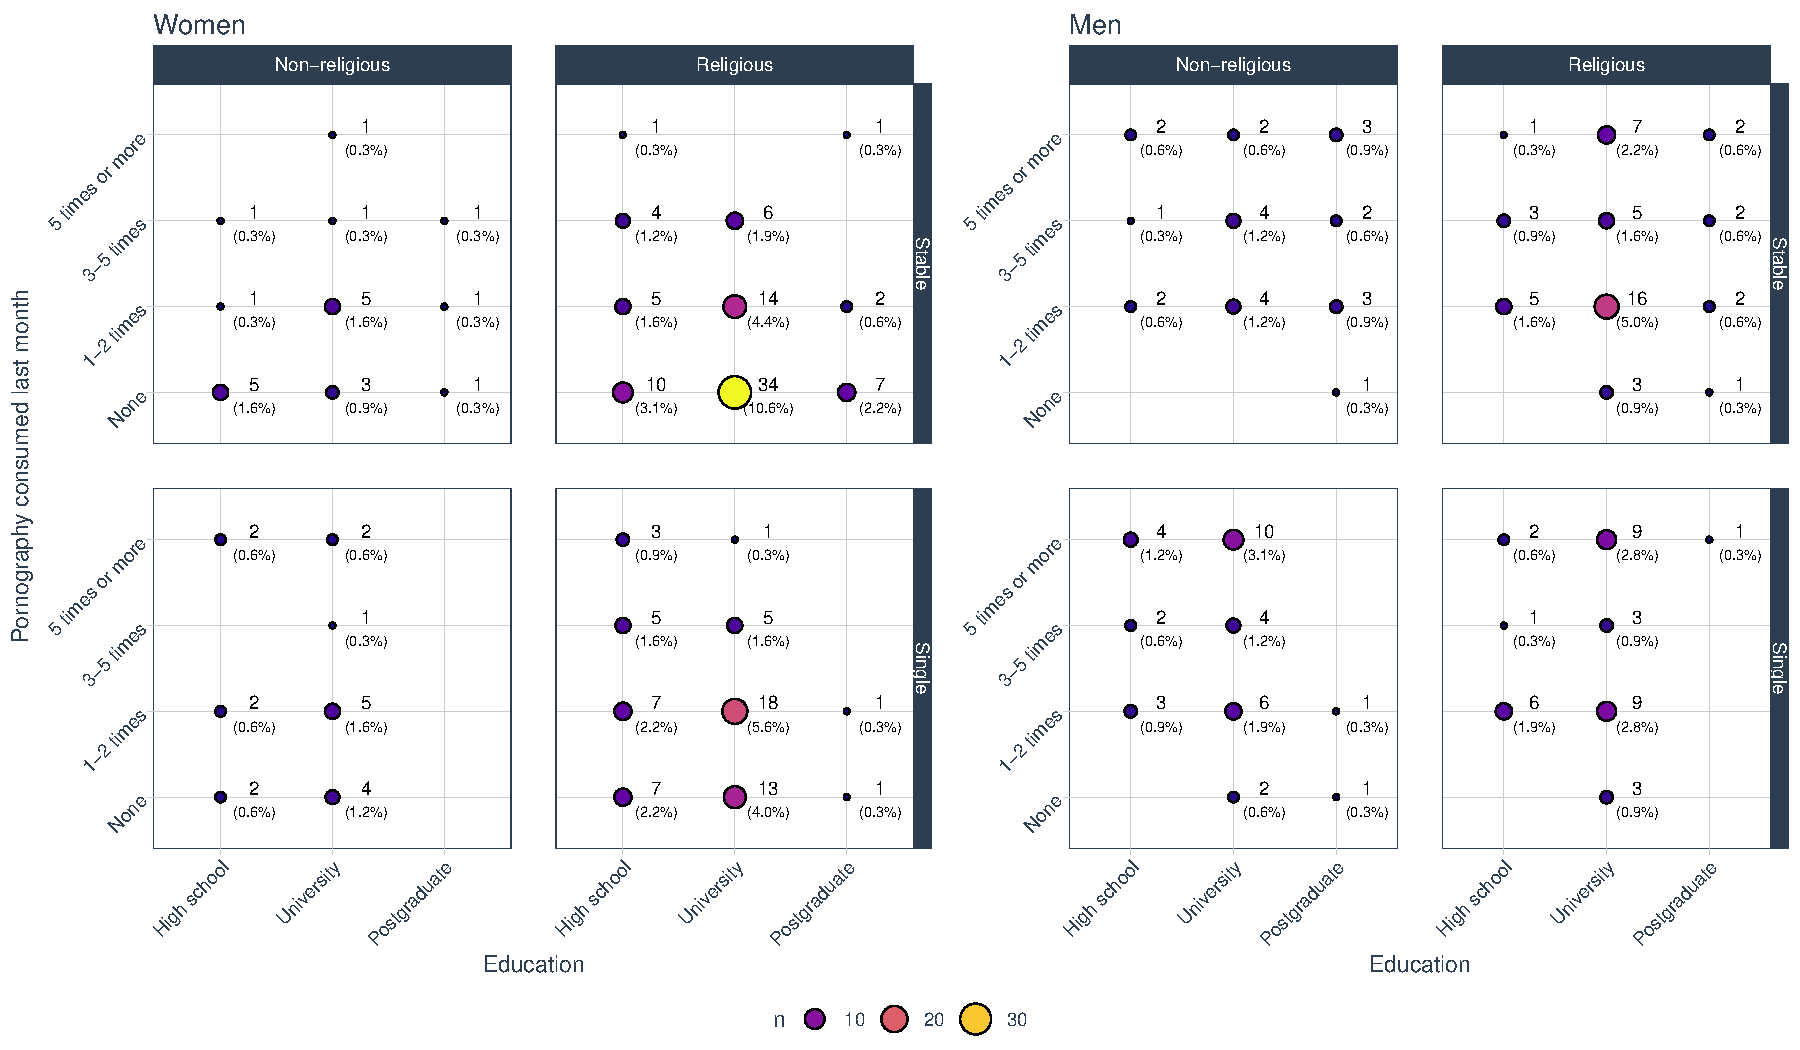
\includegraphics{Sexual_Desire_Arousal_anonymous_files/figure-latex/sample-plot-1.pdf}
\caption{\label{fig:sample-plot}Number of participants by gender (left = women, rigth = men), Relationship (stable = top panels, single = bottom panels), Religion (non-religious = left panels by gender, religious = right panels by gender), Education (\emph{X} axis), and pornography consumed during the last month (\emph{Y} axis). The number of participants for each combination of these five variables is displayed as numbers (percentage in brackets), as well as by the color and size of the bubbles .}
\end{figure}

\subsection{Descriptive statistics of the participants by gender}\label{descriptive-statistics-of-the-participants-by-gender}

Calculate mean values per participant for relevant, numeric variables.

\begin{Shaded}
\begin{Highlighting}[]
\CommentTok{\# Compute mean values per participant for selected numeric variables}
\NormalTok{dat.desc }\OtherTok{\textless{}{-}}\NormalTok{ dat }\SpecialCharTok{|\textgreater{}}
  \FunctionTok{select}\NormalTok{(}
\NormalTok{    Participant, Gender, Age, Relationship, }\StringTok{\textasciigrave{}}\AttributeTok{Number of sexual partners}\StringTok{\textasciigrave{}}\NormalTok{,}
    \StringTok{\textasciigrave{}}\AttributeTok{MGH{-}SFQ (total)}\StringTok{\textasciigrave{}}\NormalTok{,}
    \StringTok{\textasciigrave{}}\AttributeTok{MGSS sexual satisfaction (General)}\StringTok{\textasciigrave{}}\NormalTok{, }\StringTok{\textasciigrave{}}\AttributeTok{MGSS sexual satisfaction (Partner)}\StringTok{\textasciigrave{}}\NormalTok{,}
    \StringTok{\textasciigrave{}}\AttributeTok{Subjective sexual attractiveness}\StringTok{\textasciigrave{}}\NormalTok{, }\StringTok{\textasciigrave{}}\AttributeTok{Subjective sexual arousal}\StringTok{\textasciigrave{}}\NormalTok{,}
    \StringTok{\textasciigrave{}}\AttributeTok{Solitary sexual desire}\StringTok{\textasciigrave{}}\NormalTok{,}
    \StringTok{\textasciigrave{}}\AttributeTok{Dyadic sexual desire (Attractive person)}\StringTok{\textasciigrave{}}\NormalTok{, }\StringTok{\textasciigrave{}}\AttributeTok{Dyadic sexual desire (Partner)}\StringTok{\textasciigrave{}}
\NormalTok{  ) }\SpecialCharTok{|\textgreater{}}
  \FunctionTok{group\_by}\NormalTok{(Participant, Gender, Relationship) }\SpecialCharTok{|\textgreater{}} \CommentTok{\# Group by participant, gender, relationship}
  \FunctionTok{summarize\_if}\NormalTok{(is.numeric, mean, }\AttributeTok{na.rm =} \ConstantTok{TRUE}\NormalTok{) }\CommentTok{\# Compute mean for numeric variables}
\end{Highlighting}
\end{Shaded}

\subsubsection{Table \ref{tab:desciptive-tab}. Descriptive statistics of the participants by gender}\label{table-reftabdesciptive-tab.-descriptive-statistics-of-the-participants-by-gender}

Table of descriptives by gender.

\begin{Shaded}
\begin{Highlighting}[]
\CommentTok{\# Generate a table of descriptive statistics by gender and relationship status}
\FunctionTok{describeBy}\NormalTok{(dat.desc }\SpecialCharTok{\textasciitilde{}}\NormalTok{ Relationship }\SpecialCharTok{+}\NormalTok{ Gender,}
  \AttributeTok{mat =} \ConstantTok{TRUE}\NormalTok{, }\AttributeTok{digits =} \DecValTok{2} \CommentTok{\# Convert output to a matrix, round to 2 decimal places}
\NormalTok{) }\SpecialCharTok{|\textgreater{}}
  \FunctionTok{rownames\_to\_column}\NormalTok{(}\StringTok{"Measured characteristic"}\NormalTok{) }\SpecialCharTok{|\textgreater{}} \CommentTok{\# Move row names to a column}
  \FunctionTok{select}\NormalTok{(}\DecValTok{1}\NormalTok{, }\DecValTok{3}\SpecialCharTok{:}\DecValTok{4}\NormalTok{, }\DecValTok{6}\SpecialCharTok{:}\DecValTok{9}\NormalTok{, }\DecValTok{12}\SpecialCharTok{:}\DecValTok{13}\NormalTok{) }\SpecialCharTok{|\textgreater{}} \CommentTok{\# Select relevant columns}
  \FunctionTok{slice}\NormalTok{(}\SpecialCharTok{{-}}\NormalTok{(}\DecValTok{1}\SpecialCharTok{:}\DecValTok{12}\NormalTok{)) }\SpecialCharTok{|\textgreater{}} \CommentTok{\# Remove unnecessary rows}
  \FunctionTok{select}\NormalTok{(}\DecValTok{1}\NormalTok{, }\DecValTok{3}\NormalTok{, }\DecValTok{2}\NormalTok{, }\DecValTok{4}\SpecialCharTok{:}\DecValTok{9}\NormalTok{) }\SpecialCharTok{|\textgreater{}} \CommentTok{\# Reorder columns for better readability}
  \CommentTok{\# Remove numeric suffixes from row names (now in the "Measured characteristic" column)}
  \FunctionTok{mutate}\NormalTok{(}\StringTok{"Measured characteristic"} \OtherTok{=} \FunctionTok{str\_replace\_all}\NormalTok{(}
    \StringTok{\textasciigrave{}}\AttributeTok{Measured characteristic}\StringTok{\textasciigrave{}}\NormalTok{, }\FunctionTok{c}\NormalTok{(}\StringTok{"1"} \OtherTok{=} \StringTok{""}\NormalTok{, }\StringTok{"2"} \OtherTok{=} \StringTok{""}\NormalTok{, }\StringTok{"3"} \OtherTok{=} \StringTok{""}\NormalTok{, }\StringTok{"4"} \OtherTok{=} \StringTok{""}\NormalTok{)}
\NormalTok{  )) }\SpecialCharTok{|\textgreater{}}
  \CommentTok{\# Create formatted table}
  \FunctionTok{kable}\NormalTok{(}
    \AttributeTok{digits =} \DecValTok{2}\NormalTok{, }\AttributeTok{booktabs =} \ConstantTok{TRUE}\NormalTok{, }\AttributeTok{align =} \FunctionTok{c}\NormalTok{(}\StringTok{"l"}\NormalTok{, }\StringTok{"l"}\NormalTok{, }\FunctionTok{rep}\NormalTok{(}\StringTok{"c"}\NormalTok{, }\DecValTok{7}\NormalTok{)), }
    \AttributeTok{linesep =} \StringTok{""}\NormalTok{,}
    \AttributeTok{caption =} \StringTok{"Descriptive statistics of the participants by gender and relationship status"}\NormalTok{,}
    \AttributeTok{col.names =} \FunctionTok{c}\NormalTok{(}
      \StringTok{"Measured characteristic"}\NormalTok{, }\StringTok{"Gender"}\NormalTok{, }\StringTok{"Relationship status"}\NormalTok{,}
      \StringTok{"$n$"}\NormalTok{, }\StringTok{"Mean"}\NormalTok{, }\StringTok{"$SD$"}\NormalTok{, }\StringTok{"Median"}\NormalTok{, }\StringTok{"Min"}\NormalTok{, }\StringTok{"Max"}
\NormalTok{    ),}
    \AttributeTok{longtable =} \ConstantTok{TRUE}\NormalTok{, }\AttributeTok{escape =} \ConstantTok{FALSE}
\NormalTok{  ) }\SpecialCharTok{|\textgreater{}}
  \CommentTok{\# Apply LaTeX styling}
  \FunctionTok{kable\_styling}\NormalTok{(}\AttributeTok{latex\_options =} \FunctionTok{c}\NormalTok{(}\StringTok{"HOLD\_position"}\NormalTok{), }\AttributeTok{font\_size =} \FloatTok{8.2}\NormalTok{) }\SpecialCharTok{|\textgreater{}}
  \CommentTok{\# Collapse duplicate values in the first three columns for clarity}
  \FunctionTok{collapse\_rows}\NormalTok{(}\AttributeTok{columns =} \DecValTok{1}\SpecialCharTok{:}\DecValTok{3}\NormalTok{, }\AttributeTok{valign =} \StringTok{"middle"}\NormalTok{) }\SpecialCharTok{|\textgreater{}}
  \CommentTok{\# Add a footnote explaining within{-}subject descriptives}
  \FunctionTok{footnote}\NormalTok{(}
    \AttributeTok{general =} \StringTok{"Because for }\SpecialCharTok{\textbackslash{}\textbackslash{}\textbackslash{}\textbackslash{}}\StringTok{textit\{Subjective sexual attractiveness\} and}
\StringTok{           }\SpecialCharTok{\textbackslash{}\textbackslash{}\textbackslash{}\textbackslash{}}\StringTok{textit\{Subjective sexual arousal\}, there are multiple within{-}subject}
\StringTok{           observations, descriptives are calculated from mean values per participant."}\NormalTok{,}
    \AttributeTok{threeparttable =} \ConstantTok{TRUE}\NormalTok{, }\AttributeTok{footnote\_as\_chunk =} \ConstantTok{TRUE}\NormalTok{, }\AttributeTok{escape =} \ConstantTok{FALSE}
\NormalTok{  )}
\end{Highlighting}
\end{Shaded}

\begingroup\fontsize{8.2}{10.2}\selectfont

\begin{ThreePartTable}
\begin{TableNotes}[para]
\item \textit{Note: } 
\item Because for \textit{Subjective sexual attractiveness} and
           \textit{Subjective sexual arousal}, there are multiple within-subject
           observations, descriptives are calculated from mean values per participant.
\end{TableNotes}
\begin{longtable}[t]{llccccccc}
\caption{\label{tab:desciptive-tab}Descriptive statistics of the participants by gender and relationship status}\\
\toprule
Measured characteristic & Gender & Relationship status & $n$ & Mean & $SD$ & Median & Min & Max\\
\midrule
 &  & Stable & 105 & 24.51 & 5.58 & 23.00 & 18.00 & 40.00\\
\cmidrule{3-9}\nopagebreak
 & \multirow{-2}{*}[0.5\dimexpr\aboverulesep+\belowrulesep+\cmidrulewidth]{\raggedright\arraybackslash Women} & Single & 79 & 22.27 & 3.84 & 21.00 & 18.00 & 36.00\\
\cmidrule{2-9}\nopagebreak
 &  & Stable & 72 & 26.72 & 5.64 & 25.00 & 19.00 & 40.00\\
\cmidrule{3-9}\nopagebreak
\multirow{-4}{*}[1.5\dimexpr\aboverulesep+\belowrulesep+\cmidrulewidth]{\raggedright\arraybackslash Age} & \multirow{-2}{*}[0.5\dimexpr\aboverulesep+\belowrulesep+\cmidrulewidth]{\raggedright\arraybackslash Men} & Single & 67 & 24.24 & 4.58 & 23.00 & 18.00 & 39.00\\
\cmidrule{1-9}\pagebreak[0]
 &  & Stable & 103 & 4.41 & 3.77 & 3.00 & 1.00 & 22.00\\
\cmidrule{3-9}\nopagebreak
 & \multirow{-2}{*}[0.5\dimexpr\aboverulesep+\belowrulesep+\cmidrulewidth]{\raggedright\arraybackslash Women} & Single & 76 & 5.74 & 8.85 & 3.00 & 0.00 & 63.00\\
\cmidrule{2-9}\nopagebreak
 &  & Stable & 72 & 8.72 & 11.36 & 5.00 & 1.00 & 70.00\\
\cmidrule{3-9}\nopagebreak
\multirow{-4}{*}[1.5\dimexpr\aboverulesep+\belowrulesep+\cmidrulewidth]{\raggedright\arraybackslash Number of sexual partners} & \multirow{-2}{*}[0.5\dimexpr\aboverulesep+\belowrulesep+\cmidrulewidth]{\raggedright\arraybackslash Men} & Single & 66 & 7.30 & 8.06 & 4.00 & 0.00 & 40.00\\
\cmidrule{1-9}\pagebreak[0]
 &  & Stable & 104 & 3.31 & 0.96 & 3.75 & 0.00 & 4.00\\
\cmidrule{3-9}\nopagebreak
 & \multirow{-2}{*}[0.5\dimexpr\aboverulesep+\belowrulesep+\cmidrulewidth]{\raggedright\arraybackslash Women} & Single & 79 & 2.80 & 1.23 & 3.50 & 0.00 & 4.00\\
\cmidrule{2-9}\nopagebreak
 &  & Stable & 72 & 3.59 & 0.62 & 3.90 & 0.60 & 4.00\\
\cmidrule{3-9}\nopagebreak
\multirow{-4}{*}[1.5\dimexpr\aboverulesep+\belowrulesep+\cmidrulewidth]{\raggedright\arraybackslash MGH-SFQ (total)} & \multirow{-2}{*}[0.5\dimexpr\aboverulesep+\belowrulesep+\cmidrulewidth]{\raggedright\arraybackslash Men} & Single & 67 & 3.38 & 0.83 & 3.80 & 0.60 & 4.00\\
\cmidrule{1-9}\pagebreak[0]
 &  & Stable & 100 & 25.88 & 5.67 & 28.00 & 6.00 & 30.00\\
\cmidrule{3-9}\nopagebreak
 & \multirow{-2}{*}[0.5\dimexpr\aboverulesep+\belowrulesep+\cmidrulewidth]{\raggedright\arraybackslash Women} & Single & 10 & 26.90 & 3.11 & 27.00 & 22.00 & 30.00\\
\cmidrule{2-9}\nopagebreak
 &  & Stable & 70 & 26.43 & 4.54 & 29.00 & 12.00 & 30.00\\
\cmidrule{3-9}\nopagebreak
\multirow{-4}{*}[1.5\dimexpr\aboverulesep+\belowrulesep+\cmidrulewidth]{\raggedright\arraybackslash MGSS sexual satisfaction (General)} & \multirow{-2}{*}[0.5\dimexpr\aboverulesep+\belowrulesep+\cmidrulewidth]{\raggedright\arraybackslash Men} & Single & 12 & 23.58 & 5.14 & 24.50 & 14.00 & 29.00\\
\cmidrule{1-9}\pagebreak[0]
 &  & Stable & 100 & 28.13 & 4.20 & 30.00 & 8.00 & 30.00\\
\cmidrule{3-9}\nopagebreak
 & \multirow{-2}{*}[0.5\dimexpr\aboverulesep+\belowrulesep+\cmidrulewidth]{\raggedright\arraybackslash Women} & Single & 10 & 28.10 & 2.13 & 29.00 & 25.00 & 30.00\\
\cmidrule{2-9}\nopagebreak
 &  & Stable & 70 & 28.49 & 3.48 & 30.00 & 6.00 & 30.00\\
\cmidrule{3-9}\nopagebreak
\multirow{-4}{*}[1.5\dimexpr\aboverulesep+\belowrulesep+\cmidrulewidth]{\raggedright\arraybackslash MGSS sexual satisfaction (Partner)} & \multirow{-2}{*}[0.5\dimexpr\aboverulesep+\belowrulesep+\cmidrulewidth]{\raggedright\arraybackslash Men} & Single & 12 & 26.08 & 4.85 & 27.50 & 15.00 & 30.00\\
\cmidrule{1-9}\pagebreak[0]
 &  & Stable & 105 & 2.94 & 1.11 & 2.78 & 1.00 & 5.49\\
\cmidrule{3-9}\nopagebreak
 & \multirow{-2}{*}[0.5\dimexpr\aboverulesep+\belowrulesep+\cmidrulewidth]{\raggedright\arraybackslash Women} & Single & 79 & 3.19 & 1.06 & 3.11 & 1.44 & 6.77\\
\cmidrule{2-9}\nopagebreak
 &  & Stable & 72 & 3.27 & 0.94 & 3.24 & 1.11 & 6.20\\
\cmidrule{3-9}\nopagebreak
\multirow{-4}{*}[1.5\dimexpr\aboverulesep+\belowrulesep+\cmidrulewidth]{\raggedright\arraybackslash Subjective sexual attractiveness} & \multirow{-2}{*}[0.5\dimexpr\aboverulesep+\belowrulesep+\cmidrulewidth]{\raggedright\arraybackslash Men} & Single & 67 & 3.20 & 0.90 & 3.18 & 1.09 & 5.72\\
\cmidrule{1-9}\pagebreak[0]
 &  & Stable & 105 & 1.59 & 0.68 & 1.39 & 1.00 & 4.21\\
\cmidrule{3-9}\nopagebreak
 & \multirow{-2}{*}[0.5\dimexpr\aboverulesep+\belowrulesep+\cmidrulewidth]{\raggedright\arraybackslash Women} & Single & 79 & 1.75 & 0.71 & 1.52 & 1.00 & 4.39\\
\cmidrule{2-9}\nopagebreak
 &  & Stable & 72 & 2.24 & 0.83 & 2.07 & 1.00 & 4.57\\
\cmidrule{3-9}\nopagebreak
\multirow{-4}{*}[1.5\dimexpr\aboverulesep+\belowrulesep+\cmidrulewidth]{\raggedright\arraybackslash Subjective sexual arousal} & \multirow{-2}{*}[0.5\dimexpr\aboverulesep+\belowrulesep+\cmidrulewidth]{\raggedright\arraybackslash Men} & Single & 67 & 2.16 & 0.78 & 2.05 & 1.00 & 4.09\\
\cmidrule{1-9}\pagebreak[0]
 &  & Stable & 105 & 11.53 & 8.59 & 12.00 & 0.00 & 29.00\\
\cmidrule{3-9}\nopagebreak
 & \multirow{-2}{*}[0.5\dimexpr\aboverulesep+\belowrulesep+\cmidrulewidth]{\raggedright\arraybackslash Women} & Single & 79 & 16.03 & 8.35 & 17.00 & 0.00 & 31.00\\
\cmidrule{2-9}\nopagebreak
 &  & Stable & 72 & 17.47 & 7.51 & 17.50 & 0.00 & 31.00\\
\cmidrule{3-9}\nopagebreak
\multirow{-4}{*}[1.5\dimexpr\aboverulesep+\belowrulesep+\cmidrulewidth]{\raggedright\arraybackslash Solitary sexual desire} & \multirow{-2}{*}[0.5\dimexpr\aboverulesep+\belowrulesep+\cmidrulewidth]{\raggedright\arraybackslash Men} & Single & 67 & 18.25 & 7.10 & 19.00 & 1.00 & 31.00\\
\cmidrule{1-9}\pagebreak[0]
 &  & Stable & 105 & 10.55 & 7.64 & 10.00 & 0.00 & 30.00\\
\cmidrule{3-9}\nopagebreak
 & \multirow{-2}{*}[0.5\dimexpr\aboverulesep+\belowrulesep+\cmidrulewidth]{\raggedright\arraybackslash Women} & Single & 79 & 14.06 & 7.39 & 15.00 & 0.00 & 32.00\\
\cmidrule{2-9}\nopagebreak
 &  & Stable & 72 & 16.21 & 7.44 & 15.50 & 0.00 & 32.00\\
\cmidrule{3-9}\nopagebreak
\multirow{-4}{*}[1.5\dimexpr\aboverulesep+\belowrulesep+\cmidrulewidth]{\raggedright\arraybackslash Dyadic sexual desire (Attractive person)} & \multirow{-2}{*}[0.5\dimexpr\aboverulesep+\belowrulesep+\cmidrulewidth]{\raggedright\arraybackslash Men} & Single & 67 & 17.57 & 6.66 & 17.00 & 2.00 & 30.00\\
\cmidrule{1-9}\pagebreak[0]
 &  & Stable & 105 & 27.53 & 8.50 & 30.00 & 0.00 & 38.00\\
\cmidrule{3-9}\nopagebreak
 & \multirow{-2}{*}[0.5\dimexpr\aboverulesep+\belowrulesep+\cmidrulewidth]{\raggedright\arraybackslash Women} & Single & 76 & 21.33 & 10.91 & 23.00 & 0.00 & 38.00\\
\cmidrule{2-9}\nopagebreak
 &  & Stable & 72 & 31.35 & 5.33 & 32.00 & 15.00 & 38.00\\
\cmidrule{3-9}\nopagebreak
\multirow{-4}{*}[1.5\dimexpr\aboverulesep+\belowrulesep+\cmidrulewidth]{\raggedright\arraybackslash Dyadic sexual desire (Partner)} & \multirow{-2}{*}[0.5\dimexpr\aboverulesep+\belowrulesep+\cmidrulewidth]{\raggedright\arraybackslash Men} & Single & 67 & 25.81 & 9.40 & 28.00 & 0.00 & 38.00\\
\bottomrule
\insertTableNotes
\end{longtable}
\end{ThreePartTable}
\endgroup{}

\subsubsection{Figure \ref{fig:density-plot}. Distribution of participants' measured variables by gender}\label{figure-reffigdensity-plot.-distribution-of-participants-measured-variables-by-gender}

Kernel density distributions by gender.

\begin{Shaded}
\begin{Highlighting}[]
\CommentTok{\# Convert dat.desc to long format for easier plotting}
\NormalTok{datp }\OtherTok{\textless{}{-}}\NormalTok{ dat.desc }\SpecialCharTok{|\textgreater{}}
  \FunctionTok{pivot\_longer}\NormalTok{(}
    \AttributeTok{cols =}\NormalTok{ Age}\SpecialCharTok{:}\StringTok{\textasciigrave{}}\AttributeTok{Dyadic sexual desire (Partner)}\StringTok{\textasciigrave{}}\NormalTok{, }\CommentTok{\# Convert selected columns to long format}
    \AttributeTok{names\_to =} \StringTok{"Variable"}\NormalTok{, }\AttributeTok{values\_to =} \StringTok{"Value"}
\NormalTok{  ) }\SpecialCharTok{|\textgreater{}}
  \FunctionTok{mutate}\NormalTok{(}\AttributeTok{Variable =} \FunctionTok{str\_wrap}\NormalTok{(Variable, }\AttributeTok{width =} \DecValTok{30}\NormalTok{)) }\CommentTok{\# Wrap variable names for better display}

\CommentTok{\# Panel 1: Age, Sexual Partners, and Subjective Sexual Measures}
\NormalTok{fs2a }\OtherTok{\textless{}{-}} \FunctionTok{ggplot}\NormalTok{(}
\NormalTok{  datp }\SpecialCharTok{|\textgreater{}} \FunctionTok{filter}\NormalTok{(Variable }\SpecialCharTok{\%in\%} \FunctionTok{c}\NormalTok{(}
    \StringTok{"Age"}\NormalTok{, }\StringTok{"Number of sexual partners"}\NormalTok{,}
    \StringTok{"Subjective sexual}\SpecialCharTok{\textbackslash{}n}\StringTok{attractiveness"}\NormalTok{, }\StringTok{"Subjective sexual arousal"}
\NormalTok{  )),}
  \FunctionTok{aes}\NormalTok{(Value, }\AttributeTok{fill =}\NormalTok{ Gender, }\AttributeTok{colour =}\NormalTok{ Gender)}
\NormalTok{) }\SpecialCharTok{+}
  \FunctionTok{geom\_density}\NormalTok{(}\AttributeTok{alpha =} \FloatTok{0.3}\NormalTok{) }\SpecialCharTok{+} \CommentTok{\# Density plot with transparency}
  \FunctionTok{geom\_vline}\NormalTok{(}
    \AttributeTok{data =}\NormalTok{ datp }\SpecialCharTok{|\textgreater{}}
      \FunctionTok{filter}\NormalTok{(Variable }\SpecialCharTok{\%in\%} \FunctionTok{c}\NormalTok{(}
        \StringTok{"Age"}\NormalTok{, }\StringTok{"Number of sexual partners"}\NormalTok{,}
        \StringTok{"Subjective sexual}\SpecialCharTok{\textbackslash{}n}\StringTok{attractiveness"}\NormalTok{, }\StringTok{"Subjective sexual arousal"}
\NormalTok{      )) }\SpecialCharTok{|\textgreater{}}
      \FunctionTok{group\_by}\NormalTok{(Variable, Gender) }\SpecialCharTok{|\textgreater{}}
      \FunctionTok{summarise}\NormalTok{(}\AttributeTok{mean =} \FunctionTok{mean}\NormalTok{(Value, }\AttributeTok{na.rm =} \ConstantTok{TRUE}\NormalTok{)), }\CommentTok{\# Compute mean per group}
    \AttributeTok{size =} \DecValTok{1}\NormalTok{, }\FunctionTok{aes}\NormalTok{(}\AttributeTok{xintercept =}\NormalTok{ mean, }\AttributeTok{color =}\NormalTok{ Gender, }\AttributeTok{linetype =}\NormalTok{ Gender)}
\NormalTok{  ) }\SpecialCharTok{+}
  \FunctionTok{scale\_color\_manual}\NormalTok{(}\AttributeTok{values =}\NormalTok{ color.Gender) }\SpecialCharTok{+} \CommentTok{\# Custom gender colors}
  \FunctionTok{scale\_fill\_manual}\NormalTok{(}\AttributeTok{values =}\NormalTok{ color.Gender) }\SpecialCharTok{+}
  \FunctionTok{facet\_wrap}\NormalTok{(}\SpecialCharTok{\textasciitilde{}}\NormalTok{Variable, }\AttributeTok{scales =} \StringTok{"free"}\NormalTok{, }\AttributeTok{ncol =} \DecValTok{4}\NormalTok{) }\SpecialCharTok{+} \CommentTok{\# Facet by variable}
  \FunctionTok{labs}\NormalTok{(}\AttributeTok{y =} \StringTok{"Density"}\NormalTok{, }\AttributeTok{x =} \ConstantTok{NULL}\NormalTok{) }\SpecialCharTok{+}
  \FunctionTok{theme\_tq}\NormalTok{() }\CommentTok{\# Apply tidyquant theme}

\CommentTok{\# Panel 2: Sexual Function and Satisfaction}
\NormalTok{fs2b }\OtherTok{\textless{}{-}} \FunctionTok{ggplot}\NormalTok{(}
\NormalTok{  datp }\SpecialCharTok{|\textgreater{}} \FunctionTok{filter}\NormalTok{(Variable }\SpecialCharTok{\%in\%} \FunctionTok{c}\NormalTok{(}
    \StringTok{"MGH{-}SFQ (total)"}\NormalTok{, }\StringTok{"MGSS sexual satisfaction}\SpecialCharTok{\textbackslash{}n}\StringTok{(General)"}\NormalTok{,}
    \StringTok{"MGSS sexual satisfaction}\SpecialCharTok{\textbackslash{}n}\StringTok{(Partner)"}
\NormalTok{  )),}
  \FunctionTok{aes}\NormalTok{(Value, }\AttributeTok{fill =}\NormalTok{ Gender, }\AttributeTok{colour =}\NormalTok{ Gender)}
\NormalTok{) }\SpecialCharTok{+}
  \FunctionTok{geom\_density}\NormalTok{(}\AttributeTok{alpha =} \FloatTok{0.3}\NormalTok{) }\SpecialCharTok{+}
  \FunctionTok{geom\_vline}\NormalTok{(}
    \AttributeTok{data =}\NormalTok{ datp }\SpecialCharTok{|\textgreater{}}
      \FunctionTok{filter}\NormalTok{(Variable }\SpecialCharTok{\%in\%} \FunctionTok{c}\NormalTok{(}
        \StringTok{"MGH{-}SFQ (total)"}\NormalTok{, }\StringTok{"MGSS sexual satisfaction}\SpecialCharTok{\textbackslash{}n}\StringTok{(General)"}\NormalTok{,}
        \StringTok{"MGSS sexual satisfaction}\SpecialCharTok{\textbackslash{}n}\StringTok{(Partner)"}
\NormalTok{      )) }\SpecialCharTok{|\textgreater{}}
      \FunctionTok{group\_by}\NormalTok{(Variable, Gender) }\SpecialCharTok{|\textgreater{}}
      \FunctionTok{summarise}\NormalTok{(}\AttributeTok{mean =} \FunctionTok{mean}\NormalTok{(Value, }\AttributeTok{na.rm =} \ConstantTok{TRUE}\NormalTok{)),}
    \AttributeTok{size =} \DecValTok{1}\NormalTok{, }\FunctionTok{aes}\NormalTok{(}\AttributeTok{xintercept =}\NormalTok{ mean, }\AttributeTok{color =}\NormalTok{ Gender, }\AttributeTok{linetype =}\NormalTok{ Gender)}
\NormalTok{  ) }\SpecialCharTok{+}
  \FunctionTok{scale\_color\_manual}\NormalTok{(}\AttributeTok{values =}\NormalTok{ color.Gender) }\SpecialCharTok{+}
  \FunctionTok{scale\_fill\_manual}\NormalTok{(}\AttributeTok{values =}\NormalTok{ color.Gender) }\SpecialCharTok{+}
  \FunctionTok{facet\_wrap}\NormalTok{(}\SpecialCharTok{\textasciitilde{}}\NormalTok{Variable, }\AttributeTok{scales =} \StringTok{"free"}\NormalTok{, }\AttributeTok{ncol =} \DecValTok{3}\NormalTok{) }\SpecialCharTok{+}
  \FunctionTok{labs}\NormalTok{(}\AttributeTok{y =} \StringTok{"Density"}\NormalTok{, }\AttributeTok{x =} \ConstantTok{NULL}\NormalTok{) }\SpecialCharTok{+}
  \FunctionTok{theme\_tq}\NormalTok{()}

\CommentTok{\# Panel 3: Sexual Desire Measures}
\NormalTok{fs2c }\OtherTok{\textless{}{-}} \FunctionTok{ggplot}\NormalTok{(}
\NormalTok{  datp }\SpecialCharTok{|\textgreater{}} \FunctionTok{filter}\NormalTok{(Variable }\SpecialCharTok{\%in\%} \FunctionTok{c}\NormalTok{(}
    \StringTok{"Solitary sexual desire"}\NormalTok{, }\StringTok{"Dyadic sexual desire}\SpecialCharTok{\textbackslash{}n}\StringTok{(Attractive person)"}\NormalTok{,}
    \StringTok{"Dyadic sexual desire (Partner)"}
\NormalTok{  )),}
  \FunctionTok{aes}\NormalTok{(Value, }\AttributeTok{fill =}\NormalTok{ Gender, }\AttributeTok{colour =}\NormalTok{ Gender)}
\NormalTok{) }\SpecialCharTok{+}
  \FunctionTok{geom\_density}\NormalTok{(}\AttributeTok{alpha =} \FloatTok{0.3}\NormalTok{) }\SpecialCharTok{+}
  \FunctionTok{geom\_vline}\NormalTok{(}
    \AttributeTok{data =}\NormalTok{ datp }\SpecialCharTok{|\textgreater{}}
      \FunctionTok{filter}\NormalTok{(Variable }\SpecialCharTok{\%in\%} \FunctionTok{c}\NormalTok{(}
        \StringTok{"Solitary sexual desire"}\NormalTok{, }\StringTok{"Dyadic sexual desire}\SpecialCharTok{\textbackslash{}n}\StringTok{(Attractive person)"}\NormalTok{,}
        \StringTok{"Dyadic sexual desire (Partner)"}
\NormalTok{      )) }\SpecialCharTok{|\textgreater{}}
      \FunctionTok{group\_by}\NormalTok{(Variable, Gender) }\SpecialCharTok{|\textgreater{}}
      \FunctionTok{summarise}\NormalTok{(}\AttributeTok{mean =} \FunctionTok{mean}\NormalTok{(Value, }\AttributeTok{na.rm =} \ConstantTok{TRUE}\NormalTok{)),}
    \AttributeTok{size =} \DecValTok{1}\NormalTok{, }\FunctionTok{aes}\NormalTok{(}\AttributeTok{xintercept =}\NormalTok{ mean, }\AttributeTok{color =}\NormalTok{ Gender, }\AttributeTok{linetype =}\NormalTok{ Gender)}
\NormalTok{  ) }\SpecialCharTok{+}
  \FunctionTok{scale\_color\_manual}\NormalTok{(}\AttributeTok{values =}\NormalTok{ color.Gender) }\SpecialCharTok{+}
  \FunctionTok{scale\_fill\_manual}\NormalTok{(}\AttributeTok{values =}\NormalTok{ color.Gender) }\SpecialCharTok{+}
  \FunctionTok{facet\_wrap}\NormalTok{(}\SpecialCharTok{\textasciitilde{}}\NormalTok{Variable, }\AttributeTok{scales =} \StringTok{"free"}\NormalTok{, }\AttributeTok{ncol =} \DecValTok{3}\NormalTok{) }\SpecialCharTok{+}
  \FunctionTok{labs}\NormalTok{(}\AttributeTok{y =} \StringTok{"Density"}\NormalTok{, }\AttributeTok{x =} \ConstantTok{NULL}\NormalTok{) }\SpecialCharTok{+}
  \FunctionTok{theme\_tq}\NormalTok{()}

\CommentTok{\# Combine the three panels into a single figure}
\FunctionTok{ggarrange}\NormalTok{(fs2a, fs2b, fs2c,}
  \AttributeTok{common.legend =} \ConstantTok{TRUE}\NormalTok{, }\AttributeTok{legend =} \StringTok{"bottom"}\NormalTok{, }\AttributeTok{nrow =} \DecValTok{3} \CommentTok{\# Common legend below, 3{-}row layout}
\NormalTok{)}
\end{Highlighting}
\end{Shaded}

\begin{figure}
\centering
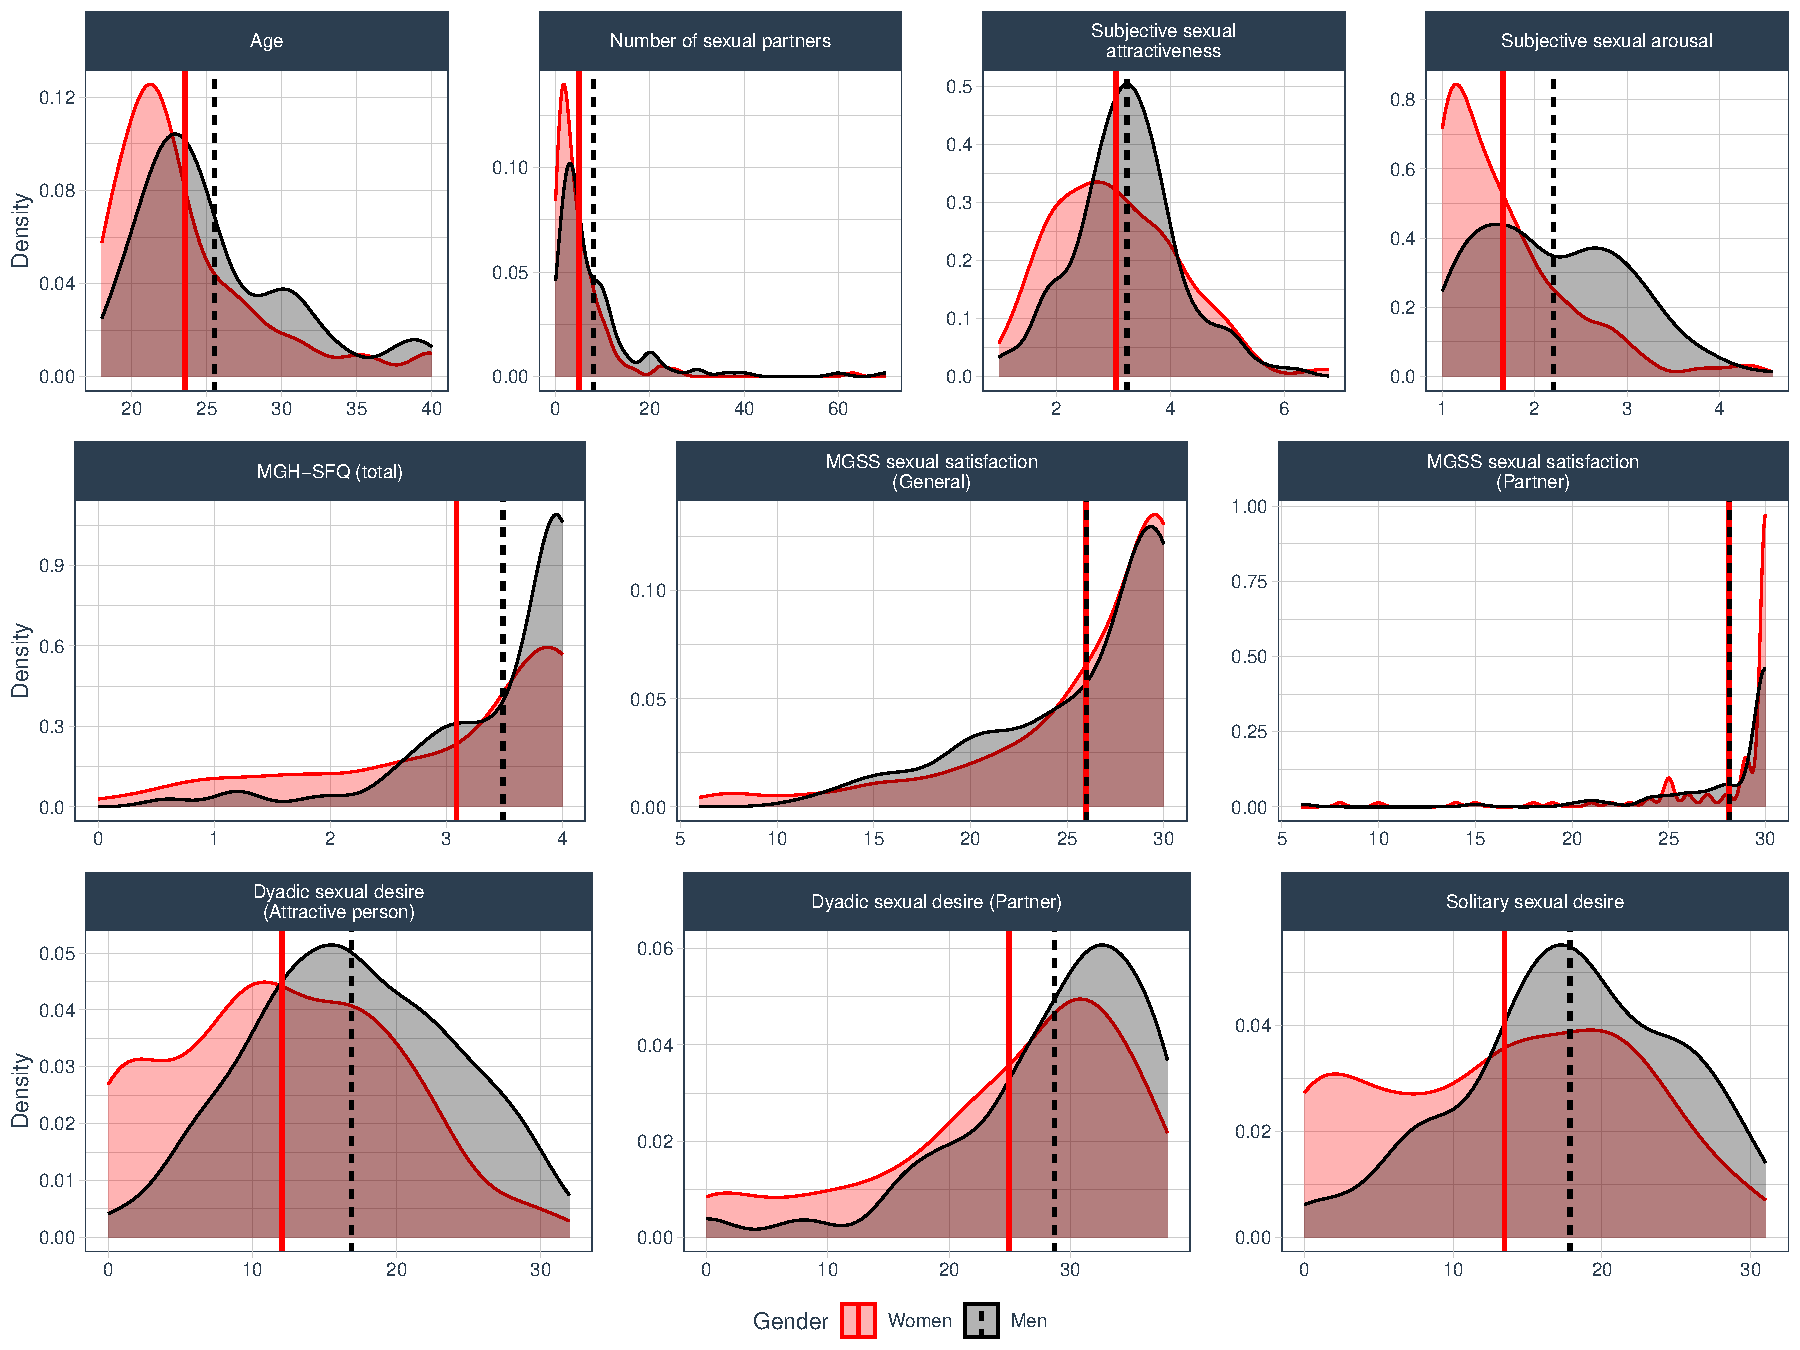
\includegraphics{Sexual_Desire_Arousal_anonymous_files/figure-latex/density-plot-1.pdf}
\caption{\label{fig:density-plot}Distribution of measured variables by gender. Coloured vertical lines represent mean values by gender. Detailed descriptives are found in Table S1. Because for \emph{Subjective sexual attractiveness} and \emph{Subjective sexual arousal} there are are multiple within-subject observations, densities calculated from mean values per participant.}
\end{figure}

\subsection{Correlations between measured variables}\label{correlations-between-measured-variables}

Correlation between numeric variables for women, men, and all participants combined, are reported in Table \ref{tab:corr-tab}.

\subsubsection{Table \ref{tab:corr-tab}. Correlations between measured variables}\label{table-reftabcorr-tab.-correlations-between-measured-variables}

Correlation matrix table.

\begin{Shaded}
\begin{Highlighting}[]
\CommentTok{\# Compute correlations for women}
\NormalTok{dat.corr.W }\OtherTok{\textless{}{-}}\NormalTok{ dat.desc }\SpecialCharTok{|\textgreater{}}
  \FunctionTok{ungroup}\NormalTok{() }\SpecialCharTok{|\textgreater{}}
  \FunctionTok{filter}\NormalTok{(Gender }\SpecialCharTok{==} \StringTok{"Women"}\NormalTok{) }\SpecialCharTok{|\textgreater{}} \CommentTok{\# Select only women}
  \FunctionTok{select}\NormalTok{(Age}\SpecialCharTok{:}\StringTok{\textasciigrave{}}\AttributeTok{Dyadic sexual desire (Partner)}\StringTok{\textasciigrave{}}\NormalTok{) }\SpecialCharTok{|\textgreater{}} \CommentTok{\# Select numeric variables}
  \FunctionTok{corr.stars}\NormalTok{() }\SpecialCharTok{|\textgreater{}} \CommentTok{\# Compute correlation matrix with significance stars}
  \FunctionTok{rownames\_to\_column}\NormalTok{(}\AttributeTok{var =} \StringTok{" "}\NormalTok{) }\CommentTok{\# Move row names to a column}

\CommentTok{\# Compute correlations for men}
\NormalTok{dat.corr.M }\OtherTok{\textless{}{-}}\NormalTok{ dat.desc }\SpecialCharTok{|\textgreater{}}
  \FunctionTok{ungroup}\NormalTok{() }\SpecialCharTok{|\textgreater{}}
  \FunctionTok{filter}\NormalTok{(Gender }\SpecialCharTok{==} \StringTok{"Men"}\NormalTok{) }\SpecialCharTok{|\textgreater{}} \CommentTok{\# Select only men}
  \FunctionTok{select}\NormalTok{(Age}\SpecialCharTok{:}\StringTok{\textasciigrave{}}\AttributeTok{Dyadic sexual desire (Partner)}\StringTok{\textasciigrave{}}\NormalTok{) }\SpecialCharTok{|\textgreater{}} \CommentTok{\# Select numeric variables}
  \FunctionTok{corr.stars}\NormalTok{() }\SpecialCharTok{|\textgreater{}}
  \FunctionTok{rownames\_to\_column}\NormalTok{(}\AttributeTok{var =} \StringTok{" "}\NormalTok{)}

\CommentTok{\# Compute correlations for all participants combined}
\NormalTok{dat.corr.All }\OtherTok{\textless{}{-}}\NormalTok{ dat.desc }\SpecialCharTok{|\textgreater{}}
  \FunctionTok{ungroup}\NormalTok{() }\SpecialCharTok{|\textgreater{}}
  \FunctionTok{select}\NormalTok{(Age}\SpecialCharTok{:}\StringTok{\textasciigrave{}}\AttributeTok{Dyadic sexual desire (Partner)}\StringTok{\textasciigrave{}}\NormalTok{) }\SpecialCharTok{|\textgreater{}}
  \FunctionTok{corr.stars}\NormalTok{() }\SpecialCharTok{|\textgreater{}}
  \FunctionTok{rownames\_to\_column}\NormalTok{(}\AttributeTok{var =} \StringTok{" "}\NormalTok{)}

\CommentTok{\# Format and combine the correlation tables}
\FunctionTok{bind\_rows}\NormalTok{(dat.corr.W, dat.corr.M, dat.corr.All) }\SpecialCharTok{|\textgreater{}}
  \FunctionTok{kable}\NormalTok{(}
    \AttributeTok{digits =} \DecValTok{2}\NormalTok{, }\AttributeTok{booktabs =} \ConstantTok{TRUE}\NormalTok{, }\AttributeTok{align =} \FunctionTok{c}\NormalTok{(}\StringTok{"l"}\NormalTok{, }\FunctionTok{rep}\NormalTok{(}\StringTok{"c"}\NormalTok{, }\DecValTok{9}\NormalTok{)), }
    \AttributeTok{linesep =} \StringTok{""}\NormalTok{,}
    \AttributeTok{caption =} \StringTok{"Correlations between measured variables"}\NormalTok{, }\AttributeTok{escape =} \ConstantTok{FALSE}
\NormalTok{  ) }\SpecialCharTok{|\textgreater{}}
  \CommentTok{\# Add grouped row labels for each participant group}
  \FunctionTok{pack\_rows}\NormalTok{(}\StringTok{"Women"}\NormalTok{,}
    \AttributeTok{start\_row =} \DecValTok{1}\NormalTok{, }\AttributeTok{end\_row =} \DecValTok{10}\NormalTok{, }\AttributeTok{bold =} \ConstantTok{FALSE}\NormalTok{,}
    \AttributeTok{background =} \StringTok{"lightgray"}
\NormalTok{  ) }\SpecialCharTok{|\textgreater{}}
  \FunctionTok{pack\_rows}\NormalTok{(}\StringTok{"Men"}\NormalTok{,}
    \AttributeTok{start\_row =} \DecValTok{11}\NormalTok{, }\AttributeTok{end\_row =} \DecValTok{20}\NormalTok{, }\AttributeTok{bold =} \ConstantTok{FALSE}\NormalTok{,}
    \AttributeTok{background =} \StringTok{"lightgray"}
\NormalTok{  ) }\SpecialCharTok{|\textgreater{}}
  \FunctionTok{pack\_rows}\NormalTok{(}\StringTok{"All participants"}\NormalTok{,}
    \AttributeTok{start\_row =} \DecValTok{21}\NormalTok{, }\AttributeTok{end\_row =} \DecValTok{30}\NormalTok{, }\AttributeTok{bold =} \ConstantTok{FALSE}\NormalTok{,}
    \AttributeTok{background =} \StringTok{"lightgray"}
\NormalTok{  ) }\SpecialCharTok{|\textgreater{}}
  \CommentTok{\# Apply LaTeX styling}
  \FunctionTok{kable\_styling}\NormalTok{(}\AttributeTok{latex\_options =} \FunctionTok{c}\NormalTok{(}\StringTok{"HOLD\_position"}\NormalTok{, }\StringTok{"scale\_down"}\NormalTok{)) }\SpecialCharTok{|\textgreater{}}
  \FunctionTok{column\_spec}\NormalTok{(}\DecValTok{2}\SpecialCharTok{:}\DecValTok{10}\NormalTok{, }\AttributeTok{width =} \StringTok{"2.2cm"}\NormalTok{) }\SpecialCharTok{|\textgreater{}} \CommentTok{\# Adjust column widths}
  \CommentTok{\# Add footnote explaining correlation significance levels}
  \FunctionTok{footnote}\NormalTok{(}
    \AttributeTok{general =} \FunctionTok{paste0}\NormalTok{(}
      \StringTok{"Values represent Pearson correlation coefficients ($r$). "}\NormalTok{,}
      \StringTok{"For significance, $\^{}\{}\SpecialCharTok{\textbackslash{}\textbackslash{}\textbackslash{}\textbackslash{}}\StringTok{dagger\}p$ \textless{} 0.1, *$p$ \textless{} 0.05, "}\NormalTok{,}
      \StringTok{"**$p$ \textless{} 0.01, ***$p$ \textless{} 0.001. "}\NormalTok{,}
      \StringTok{"Significant correlations are in bold."}
\NormalTok{    ),}
    \AttributeTok{threeparttable =} \ConstantTok{TRUE}\NormalTok{, }\AttributeTok{footnote\_as\_chunk =} \ConstantTok{TRUE}\NormalTok{, }\AttributeTok{escape =} \ConstantTok{FALSE}
\NormalTok{  ) }\SpecialCharTok{|\textgreater{}}
  \FunctionTok{landscape}\NormalTok{() }\CommentTok{\# Rotate table for better readability in LaTeX}
\end{Highlighting}
\end{Shaded}

\begin{landscape}\begin{table}[H]
\centering
\caption{\label{tab:corr-tab}Correlations between measured variables}
\centering
\resizebox{\ifdim\width>\linewidth\linewidth\else\width\fi}{!}{
\begin{threeparttable}
\begin{tabular}[t]{l>{\centering\arraybackslash}p{2.2cm}>{\centering\arraybackslash}p{2.2cm}>{\centering\arraybackslash}p{2.2cm}>{\centering\arraybackslash}p{2.2cm}>{\centering\arraybackslash}p{2.2cm}>{\centering\arraybackslash}p{2.2cm}>{\centering\arraybackslash}p{2.2cm}>{\centering\arraybackslash}p{2.2cm}>{\centering\arraybackslash}p{2.2cm}}
\toprule
  & Age & Number of sexual partners & MGH-SFQ (total) & MGSS sexual satisfaction (General) & MGSS sexual satisfaction (Partner) & Subjective sexual attractiveness & Subjective sexual arousal & Solitary sexual desire & Dyadic sexual desire (Attractive person)\\
\midrule
\addlinespace[0.3em]
\multicolumn{10}{l}{\cellcolor{lightgray}{Women}}\\
\hspace{1em}Age &  &  &  &  &  &  &  &  \vphantom{2} & \\
\hspace{1em}Number of sexual partners & \textbf{0.24**} &  &  &  &  &  &  &  & \\
\hspace{1em}MGH-SFQ (total) & -0.05 & -0.07 &  &  &  &  &  &  & \\
\hspace{1em}MGSS sexual satisfaction (General) & \textbf{-0.21*} & 0.02 & \textbf{0.46***} &  &  &  &  &  & \\
\hspace{1em}MGSS sexual satisfaction (Partner) & -0.16$^{\dagger}$ & -0.14 & \textbf{0.32***} & \textbf{0.73***} &  &  &  &  & \\
\hspace{1em}Subjective sexual attractiveness & 0.11 & \textbf{0.18*} & -0.04 & \textbf{-0.22*} & -0.18$^{\dagger}$ &  &  &  & \\
\hspace{1em}Subjective sexual arousal & 0.00 & \textbf{0.17*} & -0.13$^{\dagger}$ & -0.18$^{\dagger}$ & -0.16$^{\dagger}$ & \textbf{0.54***} &  &  & \\
\hspace{1em}Solitary sexual desire & -0.14$^{\dagger}$ & \textbf{0.28***} & 0.05 & -0.06 & -0.18$^{\dagger}$ & \textbf{0.31***} & \textbf{0.33***} &  & \\
\hspace{1em}Dyadic sexual desire (Attractive person) & 0.06 & \textbf{0.32***} & \textbf{-0.17*} & -0.04 & -0.17$^{\dagger}$ & \textbf{0.34***} & \textbf{0.36***} & \textbf{0.44***} & \\
\hspace{1em}Dyadic sexual desire (Partner) & 0.00 & \textbf{0.21**} & \textbf{0.43***} & \textbf{0.44***} & \textbf{0.27**} & 0.13$^{\dagger}$ & 0.04 & \textbf{0.31***} & 0.13$^{\dagger}$\\
\addlinespace[0.3em]
\multicolumn{10}{l}{\cellcolor{lightgray}{Men}}\\
\hspace{1em}Age &  &  &  &  &  &  &  &  \vphantom{1} & \\
\hspace{1em}Number of sexual partners & \textbf{0.23**} &  &  &  &  &  &  &  & \\
\hspace{1em}MGH-SFQ (total) & 0.04 & 0.02 &  &  &  &  &  &  & \\
\hspace{1em}MGSS sexual satisfaction (General) & \textbf{-0.24*} & -0.08 & \textbf{0.36***} &  &  &  &  &  & \\
\hspace{1em}MGSS sexual satisfaction (Partner) & -0.13 & -0.01 & 0.10 & \textbf{0.63***} &  &  &  &  & \\
\hspace{1em}Subjective sexual attractiveness & 0.10 & -0.05 & -0.08 & -0.10 & -0.02 &  &  &  & \\
\hspace{1em}Subjective sexual arousal & \textbf{0.2*} & 0.07 & 0.05 & -0.14 & -0.09 & \textbf{0.46***} &  &  & \\
\hspace{1em}Solitary sexual desire & -0.16$^{\dagger}$ & 0.00 & 0.09 & 0.10 & 0.17 & \textbf{0.26**} & 0.11 &  & \\
\hspace{1em}Dyadic sexual desire (Attractive person) & 0.12 & \textbf{0.29***} & 0.03 & -0.13 & -0.08 & \textbf{0.25**} & \textbf{0.43***} & \textbf{0.25**} & \\
\hspace{1em}Dyadic sexual desire (Partner) & 0.11 & 0.07 & \textbf{0.36***} & \textbf{0.55***} & \textbf{0.22*} & 0.14 & \textbf{0.24**} & \textbf{0.17*} & \textbf{0.2*}\\
\addlinespace[0.3em]
\multicolumn{10}{l}{\cellcolor{lightgray}{All participants}}\\
\hspace{1em}Age &  &  &  &  &  &  &  &  & \\
\hspace{1em}Number of sexual partners & \textbf{0.26***} &  &  &  &  &  &  &  & \\
\hspace{1em}MGH-SFQ (total) & 0.02 & 0.01 &  &  &  &  &  &  & \\
\hspace{1em}MGSS sexual satisfaction (General) & \textbf{-0.22**} & -0.03 & \textbf{0.42***} &  &  &  &  &  & \\
\hspace{1em}MGSS sexual satisfaction (Partner) & \textbf{-0.14*} & -0.07 & \textbf{0.24***} & \textbf{0.69***} &  &  &  &  & \\
\hspace{1em}Subjective sexual attractiveness & \textbf{0.12*} & 0.08 & -0.03 & \textbf{-0.18*} & -0.12 &  &  &  & \\
\hspace{1em}Subjective sexual arousal & \textbf{0.15**} & \textbf{0.17**} & 0.01 & \textbf{-0.15*} & -0.12$^{\dagger}$ & \textbf{0.5***} &  &  & \\
\hspace{1em}Solitary sexual desire & -0.09 & \textbf{0.17**} & 0.11$^{\dagger}$ & 0.00 & -0.05 & \textbf{0.31***} & \textbf{0.3***} &  & \\
\hspace{1em}Dyadic sexual desire (Attractive person) & \textbf{0.14*} & \textbf{0.33***} & -0.04 & -0.07 & -0.12$^{\dagger}$ & \textbf{0.32***} & \textbf{0.45***} & \textbf{0.42***} & \\
\hspace{1em}Dyadic sexual desire (Partner) & 0.08 & \textbf{0.16**} & \textbf{0.43***} & \textbf{0.46***} & \textbf{0.25***} & \textbf{0.15**} & \textbf{0.18**} & \textbf{0.3***} & \textbf{0.21***}\\
\bottomrule
\end{tabular}
\begin{tablenotes}[para]
\item \textit{Note: } 
\item Values represent Pearson correlation coefficients ($r$). For significance, $^{\dagger}p$ < 0.1, *$p$ < 0.05, **$p$ < 0.01, ***$p$ < 0.001. Significant correlations are in bold.
\end{tablenotes}
\end{threeparttable}}
\end{table}
\end{landscape}

\subsection{Internal consistency}\label{internal-consistency}

Six variables were calculated from multiple items (1. MGH-SFQ, 2. Dyadic sexual desire (Partner), 3. Solitary sexual desire, 4. Dyadic sexual desire (Attractive person), 5. MGSS sexual satisfaction (General) and 6. MGSS sexual satisfaction (Partner)).

Data by item, for each participant, is included in the following data base, loaded as \texttt{dat.reli}:

\begin{Shaded}
\begin{Highlighting}[]
\CommentTok{\# Load dataset containing item{-}level data for internal consistency analysis}
\NormalTok{dat.reli }\OtherTok{\textless{}{-}} \FunctionTok{read\_excel}\NormalTok{(}\StringTok{"data/BD\_ConsistenciaInterna.xlsx"}\NormalTok{) }\SpecialCharTok{|\textgreater{}}
  \CommentTok{\# Recode gender variable: 1 = Men, 2 = Women}
  \FunctionTok{mutate}\NormalTok{(}\AttributeTok{Sex =} \FunctionTok{recode\_factor}\NormalTok{(Sex, }\StringTok{"2"} \OtherTok{=} \StringTok{"Women"}\NormalTok{, }\StringTok{"1"} \OtherTok{=} \StringTok{"Men"}\NormalTok{)) }\SpecialCharTok{|\textgreater{}}
  \FunctionTok{rename}\NormalTok{(}\AttributeTok{Gender =}\NormalTok{ Sex) }\SpecialCharTok{|\textgreater{}} \CommentTok{\# Rename column for consistency with other datasets}
  \FunctionTok{filter}\NormalTok{(Participante }\SpecialCharTok{!=} \DecValTok{122}\NormalTok{) }\CommentTok{\# Remove participant 122 from the dataset}
\end{Highlighting}
\end{Shaded}

Participant 122 was excluded because they did not respond the psychological scales.

To measure the internal consistency of these tests, we used standardized Cronbach's alpha (\(\alpha\) or Tau-equivalent reliability: \(\rho_{T}\)) coefficients, using the function \texttt{cronbach.alpha} from the package \texttt{ltm} \autocite{LtmPackageLatent2006}.

Importantly, given that for MGH-SFQ one item was answered only by men, the internal consistency of this variable was measured independently for each gender.

\begin{Shaded}
\begin{Highlighting}[]
\CommentTok{\# Compute standardized Cronbach\textquotesingle{}s alpha (Tau{-}equivalent reliability) for each measure}

\CommentTok{\# MGH{-}SFQ for men (selects items 3 to 7, excludes missing values)}
\NormalTok{MGH.m }\OtherTok{\textless{}{-}}\NormalTok{ dat.reli }\SpecialCharTok{|\textgreater{}}
  \FunctionTok{filter}\NormalTok{(Gender }\SpecialCharTok{==} \StringTok{"Men"}\NormalTok{) }\SpecialCharTok{|\textgreater{}}
  \FunctionTok{select}\NormalTok{(}\DecValTok{3}\SpecialCharTok{:}\DecValTok{7}\NormalTok{) }\SpecialCharTok{|\textgreater{}}
  \FunctionTok{drop\_na}\NormalTok{() }\SpecialCharTok{|\textgreater{}}
  \FunctionTok{cronbach.alpha}\NormalTok{(}\AttributeTok{CI =} \ConstantTok{TRUE}\NormalTok{, }\AttributeTok{standardized =} \ConstantTok{TRUE}\NormalTok{)}

\CommentTok{\# MGH{-}SFQ for women (excludes item 6, which was answered only by men)}
\NormalTok{MGH.w }\OtherTok{\textless{}{-}}\NormalTok{ dat.reli }\SpecialCharTok{|\textgreater{}}
  \FunctionTok{filter}\NormalTok{(Gender }\SpecialCharTok{==} \StringTok{"Women"}\NormalTok{) }\SpecialCharTok{|\textgreater{}}
  \FunctionTok{select}\NormalTok{(}\DecValTok{3}\SpecialCharTok{:}\DecValTok{5}\NormalTok{, }\DecValTok{7}\NormalTok{) }\SpecialCharTok{|\textgreater{}}
  \FunctionTok{drop\_na}\NormalTok{() }\SpecialCharTok{|\textgreater{}}
  \FunctionTok{cronbach.alpha}\NormalTok{(}\AttributeTok{CI =} \ConstantTok{TRUE}\NormalTok{, }\AttributeTok{standardized =} \ConstantTok{TRUE}\NormalTok{)}

\CommentTok{\# Dyadic sexual desire (Partner) {-} items 9 to 13}
\NormalTok{DSD.p }\OtherTok{\textless{}{-}}\NormalTok{ dat.reli }\SpecialCharTok{|\textgreater{}}
  \FunctionTok{select}\NormalTok{(}\DecValTok{9}\SpecialCharTok{:}\DecValTok{13}\NormalTok{) }\SpecialCharTok{|\textgreater{}}
  \FunctionTok{drop\_na}\NormalTok{() }\SpecialCharTok{|\textgreater{}}
  \FunctionTok{cronbach.alpha}\NormalTok{(}\AttributeTok{CI =} \ConstantTok{TRUE}\NormalTok{, }\AttributeTok{standardized =} \ConstantTok{TRUE}\NormalTok{)}

\CommentTok{\# Solitary sexual desire {-} items 15 to 18}
\NormalTok{SSD.p }\OtherTok{\textless{}{-}}\NormalTok{ dat.reli }\SpecialCharTok{|\textgreater{}}
  \FunctionTok{select}\NormalTok{(}\DecValTok{15}\SpecialCharTok{:}\DecValTok{18}\NormalTok{) }\SpecialCharTok{|\textgreater{}}
  \FunctionTok{drop\_na}\NormalTok{() }\SpecialCharTok{|\textgreater{}}
  \FunctionTok{cronbach.alpha}\NormalTok{(}\AttributeTok{CI =} \ConstantTok{TRUE}\NormalTok{, }\AttributeTok{standardized =} \ConstantTok{TRUE}\NormalTok{)}

\CommentTok{\# Dyadic sexual desire (Attractive person) {-} items 20 to 23}
\NormalTok{DSD.a }\OtherTok{\textless{}{-}}\NormalTok{ dat.reli }\SpecialCharTok{|\textgreater{}}
  \FunctionTok{select}\NormalTok{(}\DecValTok{20}\SpecialCharTok{:}\DecValTok{23}\NormalTok{) }\SpecialCharTok{|\textgreater{}}
  \FunctionTok{drop\_na}\NormalTok{() }\SpecialCharTok{|\textgreater{}}
  \FunctionTok{cronbach.alpha}\NormalTok{(}\AttributeTok{CI =} \ConstantTok{TRUE}\NormalTok{, }\AttributeTok{standardized =} \ConstantTok{TRUE}\NormalTok{)}

\CommentTok{\# MGSS sexual satisfaction (General) {-} items 26 to 30}
\NormalTok{MGSS.g }\OtherTok{\textless{}{-}}\NormalTok{ dat.reli }\SpecialCharTok{|\textgreater{}}
  \FunctionTok{select}\NormalTok{(}\DecValTok{26}\SpecialCharTok{:}\DecValTok{30}\NormalTok{) }\SpecialCharTok{|\textgreater{}}
  \FunctionTok{drop\_na}\NormalTok{() }\SpecialCharTok{|\textgreater{}}
  \FunctionTok{cronbach.alpha}\NormalTok{(}\AttributeTok{CI =} \ConstantTok{TRUE}\NormalTok{, }\AttributeTok{standardized =} \ConstantTok{TRUE}\NormalTok{)}

\CommentTok{\# MGSS sexual satisfaction (Partner) {-} items 32 to 36}
\NormalTok{MGSS.p }\OtherTok{\textless{}{-}}\NormalTok{ dat.reli }\SpecialCharTok{|\textgreater{}}
  \FunctionTok{select}\NormalTok{(}\DecValTok{32}\SpecialCharTok{:}\DecValTok{36}\NormalTok{) }\SpecialCharTok{|\textgreater{}}
  \FunctionTok{drop\_na}\NormalTok{() }\SpecialCharTok{|\textgreater{}}
  \FunctionTok{cronbach.alpha}\NormalTok{(}\AttributeTok{CI =} \ConstantTok{TRUE}\NormalTok{, }\AttributeTok{standardized =} \ConstantTok{TRUE}\NormalTok{)}
\end{Highlighting}
\end{Shaded}

\subsubsection{Table \ref{tab:Cronbach-tab}. Internal consistency of construct variables}\label{table-reftabcronbach-tab.-internal-consistency-of-construct-variables}

Table of Cronbach's \(\alpha\) for construct variables.

\begin{Shaded}
\begin{Highlighting}[]
\CommentTok{\# Create a table of Cronbach\textquotesingle{}s alpha values for internal consistency analysis}
\FunctionTok{tibble}\NormalTok{(}
  \AttributeTok{Variable =} \FunctionTok{c}\NormalTok{(}
    \StringTok{"MGH{-}SFQ"}\NormalTok{, }\StringTok{"MGH{-}SFQ"}\NormalTok{,}
    \StringTok{"MGSS sexual satisfaction (General)"}\NormalTok{,}
    \StringTok{"MGSS sexual satisfaction (Partner)"}\NormalTok{,}
    \StringTok{"Dyadic TSD Partner"}\NormalTok{, }\StringTok{"Solitary TSD"}\NormalTok{,}
    \StringTok{"Dyadic TSD Attractive Person"}
\NormalTok{  ),}
  \AttributeTok{Gender =} \FunctionTok{c}\NormalTok{(}\StringTok{"Men"}\NormalTok{, }\StringTok{"Women"}\NormalTok{, }\FunctionTok{rep}\NormalTok{(}\StringTok{" "}\NormalTok{, }\DecValTok{5}\NormalTok{)), }\CommentTok{\# Report gender only for MGH{-}SFQ}
  \AttributeTok{p =} \FunctionTok{c}\NormalTok{(}
\NormalTok{    MGH.m}\SpecialCharTok{$}\NormalTok{p, MGH.w}\SpecialCharTok{$}\NormalTok{p, MGSS.g}\SpecialCharTok{$}\NormalTok{p, MGSS.p}\SpecialCharTok{$}\NormalTok{p,}
\NormalTok{    DSD.p}\SpecialCharTok{$}\NormalTok{p, SSD.p}\SpecialCharTok{$}\NormalTok{p, DSD.a}\SpecialCharTok{$}\NormalTok{p}
\NormalTok{  ),}
  \AttributeTok{n =} \FunctionTok{c}\NormalTok{(}
\NormalTok{    MGH.m}\SpecialCharTok{$}\NormalTok{n, MGH.w}\SpecialCharTok{$}\NormalTok{n, MGSS.g}\SpecialCharTok{$}\NormalTok{n, MGSS.p}\SpecialCharTok{$}\NormalTok{n,}
\NormalTok{    DSD.p}\SpecialCharTok{$}\NormalTok{n, SSD.p}\SpecialCharTok{$}\NormalTok{n, DSD.a}\SpecialCharTok{$}\NormalTok{n}
\NormalTok{  ),}
  \AttributeTok{alpha =} \FunctionTok{c}\NormalTok{(}
\NormalTok{    MGH.m}\SpecialCharTok{$}\NormalTok{alpha, MGH.w}\SpecialCharTok{$}\NormalTok{alpha, MGSS.g}\SpecialCharTok{$}\NormalTok{alpha, MGSS.p}\SpecialCharTok{$}\NormalTok{alpha,}
\NormalTok{    DSD.p}\SpecialCharTok{$}\NormalTok{alpha, SSD.p}\SpecialCharTok{$}\NormalTok{alpha, DSD.a}\SpecialCharTok{$}\NormalTok{alpha}
\NormalTok{  ),}
  \AttributeTok{ci2.5 =} \FunctionTok{c}\NormalTok{(}
\NormalTok{    MGH.m}\SpecialCharTok{$}\NormalTok{ci[}\DecValTok{1}\NormalTok{], MGH.w}\SpecialCharTok{$}\NormalTok{ci[}\DecValTok{1}\NormalTok{], MGSS.g}\SpecialCharTok{$}\NormalTok{ci[}\DecValTok{1}\NormalTok{], MGSS.p}\SpecialCharTok{$}\NormalTok{ci[}\DecValTok{1}\NormalTok{],}
\NormalTok{    DSD.p}\SpecialCharTok{$}\NormalTok{ci[}\DecValTok{1}\NormalTok{], SSD.p}\SpecialCharTok{$}\NormalTok{ci[}\DecValTok{1}\NormalTok{], DSD.a}\SpecialCharTok{$}\NormalTok{ci[}\DecValTok{1}\NormalTok{]}
\NormalTok{  ),}
  \AttributeTok{ci97.5 =} \FunctionTok{c}\NormalTok{(}
\NormalTok{    MGH.m}\SpecialCharTok{$}\NormalTok{ci[}\DecValTok{2}\NormalTok{], MGH.w}\SpecialCharTok{$}\NormalTok{ci[}\DecValTok{2}\NormalTok{], MGSS.g}\SpecialCharTok{$}\NormalTok{ci[}\DecValTok{2}\NormalTok{], MGSS.p}\SpecialCharTok{$}\NormalTok{ci[}\DecValTok{2}\NormalTok{],}
\NormalTok{    DSD.p}\SpecialCharTok{$}\NormalTok{ci[}\DecValTok{2}\NormalTok{], SSD.p}\SpecialCharTok{$}\NormalTok{ci[}\DecValTok{2}\NormalTok{], DSD.a}\SpecialCharTok{$}\NormalTok{ci[}\DecValTok{2}\NormalTok{]}
\NormalTok{  )}
\NormalTok{) }\SpecialCharTok{|\textgreater{}}
  \FunctionTok{kable}\NormalTok{(}
    \AttributeTok{digits =} \DecValTok{2}\NormalTok{, }\AttributeTok{booktabs =} \ConstantTok{TRUE}\NormalTok{, }\AttributeTok{align =} \FunctionTok{c}\NormalTok{(}\StringTok{"l"}\NormalTok{, }\StringTok{"l"}\NormalTok{, }\FunctionTok{rep}\NormalTok{(}\StringTok{"c"}\NormalTok{, }\DecValTok{5}\NormalTok{)), }
    \AttributeTok{linesep =} \StringTok{""}\NormalTok{,}
    \AttributeTok{caption =} \StringTok{"Internal consistency of measured variables"}\NormalTok{, }\AttributeTok{escape =} \ConstantTok{FALSE}\NormalTok{,}
    \AttributeTok{col.names =} \FunctionTok{c}\NormalTok{(}
      \StringTok{"Variable"}\NormalTok{, }\StringTok{"Gender"}\NormalTok{, }\StringTok{"Items"}\NormalTok{, }\StringTok{"$n$"}\NormalTok{, }\StringTok{"$}\SpecialCharTok{\textbackslash{}\textbackslash{}}\StringTok{alpha$"}\NormalTok{, }\StringTok{"$2.5}\SpecialCharTok{\textbackslash{}\textbackslash{}}\StringTok{\% CI$"}\NormalTok{, }\StringTok{"$97.5}\SpecialCharTok{\textbackslash{}\textbackslash{}}\StringTok{\% CI$"}
\NormalTok{    )}
\NormalTok{  ) }\SpecialCharTok{|\textgreater{}}
  \CommentTok{\# Merge repeated values in the "Variable" column for better readability}
  \FunctionTok{collapse\_rows}\NormalTok{(}\AttributeTok{columns =} \DecValTok{1}\NormalTok{, }\AttributeTok{valign =} \StringTok{"middle"}\NormalTok{) }\SpecialCharTok{|\textgreater{}}
  \CommentTok{\# Apply LaTeX styling for table positioning}
  \FunctionTok{kable\_styling}\NormalTok{(}\AttributeTok{latex\_options =} \StringTok{"HOLD\_position"}\NormalTok{) }\SpecialCharTok{|\textgreater{}}
  \CommentTok{\# Add footnote explaining confidence intervals and reporting choices}
  \FunctionTok{footnote}\NormalTok{(}
    \AttributeTok{general =} \StringTok{"95}\SpecialCharTok{\textbackslash{}\textbackslash{}\textbackslash{}\textbackslash{}}\StringTok{\% confidence intervals were calculated with 1,000 bootstrap samples.}
\StringTok{           Standardized Cronbach\textquotesingle{}s alpha ($}\SpecialCharTok{\textbackslash{}\textbackslash{}\textbackslash{}\textbackslash{}}\StringTok{alpha$) coefficients were computed.}
\StringTok{           MGH{-}SFQ is reported by gender, because one item was answered only by men."}\NormalTok{,}
    \AttributeTok{threeparttable =} \ConstantTok{TRUE}\NormalTok{, }\AttributeTok{footnote\_as\_chunk =} \ConstantTok{TRUE}\NormalTok{, }\AttributeTok{escape =} \ConstantTok{FALSE}
\NormalTok{  )}
\end{Highlighting}
\end{Shaded}

\begin{table}[H]
\centering
\caption{\label{tab:Cronbach-tab}Internal consistency of measured variables}
\centering
\begin{threeparttable}
\begin{tabular}[t]{llccccc}
\toprule
Variable & Gender & Items & $n$ & $\alpha$ & $2.5\% CI$ & $97.5\% CI$\\
\midrule
 & Men & 5 & 139 & 0.82 & 0.71 & 0.88\\
\cmidrule{2-7}
\multirow{-2}{*}{\raggedright\arraybackslash MGH-SFQ} & Women & 4 & 181 & 0.86 & 0.82 & 0.90\\
\cmidrule{1-7}
MGSS sexual satisfaction (General) &  & 5 & 188 & 0.92 & 0.89 & 0.94\\
\cmidrule{1-7}
MGSS sexual satisfaction (Partner) &  & 5 & 187 & 0.91 & 0.85 & 0.95\\
\cmidrule{1-7}
Dyadic TSD Partner &  & 5 & 309 & 0.90 & 0.88 & 0.92\\
\cmidrule{1-7}
Solitary TSD &  & 4 & 314 & 0.91 & 0.89 & 0.93\\
\cmidrule{1-7}
Dyadic TSD Attractive Person &  & 4 & 320 & 0.89 & 0.86 & 0.91\\
\bottomrule
\end{tabular}
\begin{tablenotes}[para]
\item \textit{Note: } 
\item 95\% confidence intervals were calculated with 1,000 bootstrap samples.
           Standardized Cronbach's alpha ($\alpha$) coefficients were computed.
           MGH-SFQ is reported by gender, because one item was answered only by men.
\end{tablenotes}
\end{threeparttable}
\end{table}

\begin{center}\rule{0.5\linewidth}{0.5pt}\end{center}

\subsection{Controlling for Relationship Duration and MGSS Sexual Satisfaction (Partner) in Sexual Desire Dimensions}\label{controlling-for-relationship-duration-and-mgss-sexual-satisfaction-partner-in-sexual-desire-dimensions}

To \textbf{ensure that the three sexual desire dimensions were not influenced by Relationship Duration or MGSS sexual satisfaction (Partner)}, we applied a three-step adjustment process:

\begin{enumerate}
\def\labelenumi{\arabic{enumi}.}
\tightlist
\item
  \textbf{Estimating the effects:}

  \begin{itemize}
  \tightlist
  \item
    We performed separate \textbf{linear regressions} where each sexual desire dimension was predicted by \textbf{Relationship Duration} and \textbf{MGSS sexual satisfaction (Partner)}.
  \item
    This allowed us to quantify how much these external factors influence each dimension.
  \end{itemize}
\item
  \textbf{Evaluating statistical significance:}

  \begin{itemize}
  \tightlist
  \item
    We conducted \textbf{Type III ANOVA} to determine which predictors had a significant effect on each sexual desire dimension.
  \item
    Only \textbf{MGSS sexual satisfaction (Partner) significantly predicted Dyadic Sexual Desire (Partner)}.
  \end{itemize}
\item
  \textbf{Removing the effects:}

  \begin{itemize}
  \tightlist
  \item
    We adjusted \textbf{only Dyadic Sexual Desire (Partner)} by extracting the \textbf{residuals} from the regression model.
  \item
    These residuals represent the \textbf{variation independent of MGSS sexual satisfaction (Partner)} and were then standardized for comparability.
  \end{itemize}
\end{enumerate}

Additionally, \textbf{MGSS sexual satisfaction (Partner) was mean-centered} before analysis.

\textbf{Step 1}: Estimating the Effects of Relationship Duration \& Partner Satisfaction

\begin{Shaded}
\begin{Highlighting}[]
\CommentTok{\# Select participants in stable relationships and ensure required variables are available}
\NormalTok{dat\_ctl }\OtherTok{\textless{}{-}}\NormalTok{ dat }\SpecialCharTok{|\textgreater{}}
  \FunctionTok{group\_by}\NormalTok{(Participant) }\SpecialCharTok{|\textgreater{}}
  \FunctionTok{slice\_head}\NormalTok{() }\SpecialCharTok{|\textgreater{}} \CommentTok{\# Retain only the first occurrence per participant}
  \FunctionTok{filter}\NormalTok{(Relationship }\SpecialCharTok{==} \StringTok{"Stable"}\NormalTok{) }\SpecialCharTok{|\textgreater{}} \CommentTok{\# Include only participants in stable relationships}
  \FunctionTok{ungroup}\NormalTok{()}

\CommentTok{\# Fit linear models predicting each sexual desire dimension}

\CommentTok{\# Model predicting Solitary TSD}
\NormalTok{ctl\_SSD }\OtherTok{\textless{}{-}} \FunctionTok{lm}\NormalTok{(}
  \StringTok{\textasciigrave{}}\AttributeTok{Solitary sexual desire}\StringTok{\textasciigrave{}} \SpecialCharTok{\textasciitilde{}} \StringTok{\textasciigrave{}}\AttributeTok{Relationship duration}\StringTok{\textasciigrave{}} \SpecialCharTok{+} \StringTok{\textasciigrave{}}\AttributeTok{MGSS sexual satisfaction (Partner)}\StringTok{\textasciigrave{}}\NormalTok{,}
  \AttributeTok{data =}\NormalTok{ dat\_ctl}
\NormalTok{)}

\CommentTok{\# Model predicting Dyadic Sexual Desire (Partner)}
\NormalTok{ctl\_PD }\OtherTok{\textless{}{-}} \FunctionTok{lm}\NormalTok{(}
  \StringTok{\textasciigrave{}}\AttributeTok{Dyadic sexual desire (Partner)}\StringTok{\textasciigrave{}} \SpecialCharTok{\textasciitilde{}} \StringTok{\textasciigrave{}}\AttributeTok{Relationship duration}\StringTok{\textasciigrave{}} \SpecialCharTok{+} 
    \StringTok{\textasciigrave{}}\AttributeTok{MGSS sexual satisfaction (Partner)}\StringTok{\textasciigrave{}}\NormalTok{,}
  \AttributeTok{data =}\NormalTok{ dat\_ctl}
\NormalTok{)}

\CommentTok{\# Model predicting Dyadic Sexual Desire (Attractive Person)}
\NormalTok{ctl\_APD }\OtherTok{\textless{}{-}} \FunctionTok{lm}\NormalTok{(}
  \StringTok{\textasciigrave{}}\AttributeTok{Dyadic sexual desire (Attractive person)}\StringTok{\textasciigrave{}} \SpecialCharTok{\textasciitilde{}} \StringTok{\textasciigrave{}}\AttributeTok{Relationship duration}\StringTok{\textasciigrave{}} \SpecialCharTok{+}
    \StringTok{\textasciigrave{}}\AttributeTok{MGSS sexual satisfaction (Partner)}\StringTok{\textasciigrave{}}\NormalTok{,}
  \AttributeTok{data =}\NormalTok{ dat\_ctl}
\NormalTok{)}
\end{Highlighting}
\end{Shaded}

\textbf{Step 2}: Displaying ANOVA Results for Each Model

The table below presents Type III ANOVA results for each model. Significant effects indicate that Relationship Duration or Partner Satisfaction meaningfully predict the corresponding sexual desire dimension.

\begin{Shaded}
\begin{Highlighting}[]
\CommentTok{\# Compute ANOVA results and effect sizes for all models}
\NormalTok{anova\_results }\OtherTok{\textless{}{-}} \FunctionTok{bind\_cols}\NormalTok{(}
  \FunctionTok{bind\_cols}\NormalTok{(}
    \FunctionTok{anova\_summary}\NormalTok{(}\FunctionTok{Anova}\NormalTok{(ctl\_SSD, }\AttributeTok{type =} \DecValTok{3}\NormalTok{)), }\CommentTok{\# Type III ANOVA for Solitary TSD}
    \FunctionTok{epsilon\_squared}\NormalTok{(ctl\_SSD) }\CommentTok{\# Compute partial epsilon squared}
\NormalTok{  ) }\SpecialCharTok{|\textgreater{}}
    \FunctionTok{unite}\NormalTok{(}\AttributeTok{col =} \StringTok{"df"}\NormalTok{, DFn}\SpecialCharTok{:}\NormalTok{DFd, }\AttributeTok{sep =} \StringTok{", "}\NormalTok{), }\CommentTok{\# Combine numerator and denominator df}
  \FunctionTok{bind\_cols}\NormalTok{(}
    \FunctionTok{anova\_summary}\NormalTok{(}\FunctionTok{Anova}\NormalTok{(ctl\_PD, }\AttributeTok{type =} \DecValTok{3}\NormalTok{)), }\CommentTok{\# Type III ANOVA for Dyadic Sexual Desire (Partner)}
    \FunctionTok{epsilon\_squared}\NormalTok{(ctl\_PD)}
\NormalTok{  ) }\SpecialCharTok{|\textgreater{}}
    \FunctionTok{unite}\NormalTok{(}\AttributeTok{col =} \StringTok{"df"}\NormalTok{, DFn}\SpecialCharTok{:}\NormalTok{DFd, }\AttributeTok{sep =} \StringTok{", "}\NormalTok{),}
  \FunctionTok{bind\_cols}\NormalTok{(}
    \FunctionTok{anova\_summary}\NormalTok{(}\FunctionTok{Anova}\NormalTok{(ctl\_APD, }\AttributeTok{type =} \DecValTok{3}\NormalTok{)), }\CommentTok{\# Type III ANOVA for Dyadic Sexual Desire (Attractive)}
    \FunctionTok{epsilon\_squared}\NormalTok{(ctl\_APD)}
\NormalTok{  ) }\SpecialCharTok{|\textgreater{}}
    \FunctionTok{unite}\NormalTok{(}\AttributeTok{col =} \StringTok{"df"}\NormalTok{, DFn}\SpecialCharTok{:}\NormalTok{DFd, }\AttributeTok{sep =} \StringTok{", "}\NormalTok{)}
\NormalTok{) }\SpecialCharTok{|\textgreater{}}
  \CommentTok{\# Remove unnecessary columns related to Sum of Squares and CI}
  \FunctionTok{select}\NormalTok{(}\SpecialCharTok{{-}}\FunctionTok{starts\_with}\NormalTok{(}\FunctionTok{c}\NormalTok{(}\StringTok{"p\textless{}.05"}\NormalTok{, }\StringTok{"ges..."}\NormalTok{, }\StringTok{"Parameter..."}\NormalTok{, }\StringTok{"CI"}\NormalTok{))) }\SpecialCharTok{|\textgreater{}}
  \CommentTok{\# Format p{-}values for LaTeX}
  \FunctionTok{mutate}\NormalTok{(}\FunctionTok{across}\NormalTok{(}\FunctionTok{starts\_with}\NormalTok{(}\StringTok{"p..."}\NormalTok{), pval.lev)) }\SpecialCharTok{|\textgreater{}}
  \FunctionTok{rename}\NormalTok{(}\AttributeTok{Effect =}\NormalTok{ Effect...}\DecValTok{1}\NormalTok{) }\SpecialCharTok{|\textgreater{}} \CommentTok{\# Rename effect column}
  \CommentTok{\# Remove redundant effect columns and clean effect names}
  \FunctionTok{select}\NormalTok{(}\SpecialCharTok{{-}}\FunctionTok{starts\_with}\NormalTok{(}\StringTok{"Effect..."}\NormalTok{)) }\SpecialCharTok{|\textgreater{}}
  \FunctionTok{mutate\_at}\NormalTok{(}\StringTok{"Effect"}\NormalTok{, str\_replace\_all, }\StringTok{"\textasciigrave{}"}\NormalTok{, }\StringTok{""}\NormalTok{)}

\CommentTok{\# Create a formatted ANOVA results table}
\NormalTok{anova\_results }\SpecialCharTok{|\textgreater{}}
  \FunctionTok{kable}\NormalTok{(}
    \AttributeTok{booktabs =} \ConstantTok{TRUE}\NormalTok{, }\AttributeTok{align =} \FunctionTok{c}\NormalTok{(}\StringTok{"l"}\NormalTok{, }\FunctionTok{rep}\NormalTok{(}\StringTok{"c"}\NormalTok{, }\DecValTok{9}\NormalTok{)), }\AttributeTok{digits =} \DecValTok{3}\NormalTok{, }\AttributeTok{escape =} \ConstantTok{FALSE}\NormalTok{,}
    \AttributeTok{caption =} \StringTok{"Effects of relationship duration and MGSS sexual satisfaction (Partner) in}
\StringTok{                   sexual desire dimensions"}\NormalTok{,}
    \AttributeTok{col.names =} \FunctionTok{c}\NormalTok{(}\StringTok{"Effect"}\NormalTok{, }\FunctionTok{rep}\NormalTok{(}\FunctionTok{c}\NormalTok{(}\StringTok{"$df$"}\NormalTok{, }\StringTok{"$F$"}\NormalTok{, }\StringTok{"$p$"}\NormalTok{, }\StringTok{"$}\SpecialCharTok{\textbackslash{}\textbackslash{}}\StringTok{epsilon\^{}2\_p$"}\NormalTok{), }\AttributeTok{times =} \DecValTok{3}\NormalTok{))}
\NormalTok{  ) }\SpecialCharTok{|\textgreater{}}
  \CommentTok{\# Apply LaTeX styling for table positioning}
  \FunctionTok{kable\_styling}\NormalTok{(}\AttributeTok{latex\_options =} \FunctionTok{c}\NormalTok{(}\StringTok{"HOLD\_position"}\NormalTok{, }\StringTok{"scale\_down"}\NormalTok{)) }\SpecialCharTok{|\textgreater{}}
  \CommentTok{\# Add section headers for the three models}
  \FunctionTok{add\_header\_above}\NormalTok{(}\FunctionTok{c}\NormalTok{(}
    \StringTok{" "} \OtherTok{=} \DecValTok{1}\NormalTok{,}
    \StringTok{"Solitary sexual desire"} \OtherTok{=} \DecValTok{4}\NormalTok{,}
    \StringTok{"Dyadic sexual desire}\SpecialCharTok{\textbackslash{}n}\StringTok{(Partner)"} \OtherTok{=} \DecValTok{4}\NormalTok{,}
    \StringTok{"Dyadic sexual desire}\SpecialCharTok{\textbackslash{}n}\StringTok{(Attractive person)"} \OtherTok{=} \DecValTok{4}
\NormalTok{  )) }\SpecialCharTok{|\textgreater{}}
  \CommentTok{\# Add footnote explaining effect sizes and significance}
  \FunctionTok{footnote}\NormalTok{(}
    \AttributeTok{general =} \StringTok{"As effect size, we report partial epsilon squared}
\StringTok{                     ($}\SpecialCharTok{\textbackslash{}\textbackslash{}\textbackslash{}\textbackslash{}}\StringTok{epsilon\^{}2\_p$), which provides a less biased}
\StringTok{                     estimate than $}\SpecialCharTok{\textbackslash{}\textbackslash{}\textbackslash{}\textbackslash{}}\StringTok{eta\^{}2$ (see}
\StringTok{                     }\SpecialCharTok{\textbackslash{}\textbackslash{}\textbackslash{}\textbackslash{}}\StringTok{cite\{albersWhenPowerAnalyses2018\}).}
\StringTok{                     Significant effects are in bold."}\NormalTok{,}
    \AttributeTok{threeparttable =} \ConstantTok{TRUE}\NormalTok{, }\AttributeTok{footnote\_as\_chunk =} \ConstantTok{TRUE}\NormalTok{, }\AttributeTok{escape =} \ConstantTok{FALSE}
\NormalTok{  )}
\end{Highlighting}
\end{Shaded}

\begin{table}[H]
\centering
\caption{\label{tab:unnamed-chunk-13}Effects of relationship duration and MGSS sexual satisfaction (Partner) in
                   sexual desire dimensions}
\centering
\resizebox{\ifdim\width>\linewidth\linewidth\else\width\fi}{!}{
\begin{threeparttable}
\begin{tabular}[t]{lccccccccclcc}
\toprule
\multicolumn{1}{c}{ } & \multicolumn{4}{c}{Solitary sexual desire} & \multicolumn{4}{c}{\makecell[c]{Dyadic sexual desire\\(Partner)}} & \multicolumn{4}{c}{\makecell[c]{Dyadic sexual desire\\(Attractive person)}} \\
\cmidrule(l{3pt}r{3pt}){2-5} \cmidrule(l{3pt}r{3pt}){6-9} \cmidrule(l{3pt}r{3pt}){10-13}
Effect & $df$ & $F$ & $p$ & $\epsilon^2_p$ & $df$ & $F$ & $p$ & $\epsilon^2_p$ & $df$ & $F$ & $p$ & $\epsilon^2_p$\\
\midrule
Relationship duration & 3, 165 & 0.482 & 0.70 & 0 & 3, 165 & 2.081 & 0.1 & 0.041 & 3, 165 & 0.095 & 0.96 & 0\\
MGSS sexual satisfaction (Partner) & 1, 165 & 0.029 & 0.86 & 0 & 1, 165 & 8.875 & \textbf{0.003} & 0.045 & 1, 165 & 0.884 & 0.35 & 0\\
\bottomrule
\end{tabular}
\begin{tablenotes}[para]
\item \textit{Note: } 
\item As effect size, we report partial epsilon squared
                     ($\epsilon^2_p$), which provides a less biased
                     estimate than $\eta^2$ (see
                     \cite{albersWhenPowerAnalyses2018}).
                     Significant effects are in bold.
\end{tablenotes}
\end{threeparttable}}
\end{table}

\textbf{Step 3}: Controlling Scores Based on ANOVA Results

From the ANOVA results, only the effect of MGSS sexual satisfaction (Partner) on Dyadic sexual desire (Partner) was significant. Thus, only Dyadic Sexual Desire (Partner) scores were adjusted, while the other dimensions remained unchanged.

\begin{Shaded}
\begin{Highlighting}[]
\CommentTok{\# Prepare dataset with relevant variables and remove missing values}
\NormalTok{dat\_tl\_PD\_fin }\OtherTok{\textless{}{-}}\NormalTok{ dat\_ctl }\SpecialCharTok{|\textgreater{}}
  \FunctionTok{select}\NormalTok{(}
\NormalTok{    Participant, }\StringTok{\textasciigrave{}}\AttributeTok{Dyadic sexual desire (Partner)}\StringTok{\textasciigrave{}}\NormalTok{, }\StringTok{\textasciigrave{}}\AttributeTok{MGSS sexual satisfaction (Partner)}\StringTok{\textasciigrave{}}
\NormalTok{  ) }\SpecialCharTok{|\textgreater{}}
  \FunctionTok{drop\_na}\NormalTok{() }\CommentTok{\# Remove rows with missing values}

\CommentTok{\# Fit a linear model predicting Dyadic Sexual Desire (Partner) using partner satisfaction}
\NormalTok{ctl\_PD\_fin }\OtherTok{\textless{}{-}} \FunctionTok{lm}\NormalTok{(}
  \StringTok{\textasciigrave{}}\AttributeTok{Dyadic sexual desire (Partner)}\StringTok{\textasciigrave{}} \SpecialCharTok{\textasciitilde{}} \StringTok{\textasciigrave{}}\AttributeTok{MGSS sexual satisfaction (Partner)}\StringTok{\textasciigrave{}}\NormalTok{,}
  \AttributeTok{data =}\NormalTok{ dat\_tl\_PD\_fin}
\NormalTok{)}

\CommentTok{\# Adjust Dyadic Sexual Desire (Partner) scores using residuals from the regression model}
\NormalTok{dat\_ctl }\OtherTok{\textless{}{-}}\NormalTok{ dat\_tl\_PD\_fin }\SpecialCharTok{|\textgreater{}}
  \FunctionTok{mutate}\NormalTok{(}
    \StringTok{\textasciigrave{}}\AttributeTok{Dyadic sexual desire (Partner)}\StringTok{\textasciigrave{}} \OtherTok{=}
      \FunctionTok{mean}\NormalTok{(}\StringTok{\textasciigrave{}}\AttributeTok{Dyadic sexual desire (Partner)}\StringTok{\textasciigrave{}}\NormalTok{) }\SpecialCharTok{+} \FunctionTok{resid}\NormalTok{(ctl\_PD\_fin) }\CommentTok{\# Centered residuals}
\NormalTok{  )}

\CommentTok{\# Update the original dataset with adjusted scores for Dyadic Sexual Desire (Partner)}
\NormalTok{dat }\OtherTok{\textless{}{-}}\NormalTok{ dat }\SpecialCharTok{|\textgreater{}}
  \FunctionTok{mutate}\NormalTok{(}\StringTok{\textasciigrave{}}\AttributeTok{Dyadic sexual desire (Partner)}\StringTok{\textasciigrave{}} \OtherTok{=} \FunctionTok{as.numeric}\NormalTok{(}\StringTok{\textasciigrave{}}\AttributeTok{Dyadic sexual desire (Partner)}\StringTok{\textasciigrave{}}\NormalTok{)) }\SpecialCharTok{|\textgreater{}}
  \FunctionTok{rows\_update}\NormalTok{(}
\NormalTok{    dat\_ctl }\SpecialCharTok{|\textgreater{}} \FunctionTok{select}\NormalTok{(}\SpecialCharTok{{-}}\StringTok{\textasciigrave{}}\AttributeTok{MGSS sexual satisfaction (Partner)}\StringTok{\textasciigrave{}}\NormalTok{), }\CommentTok{\# Remove predictor column}
    \AttributeTok{by =} \StringTok{"Participant"}\NormalTok{, }\AttributeTok{unmatched =} \StringTok{"ignore"} \CommentTok{\# Match by participant ID}
\NormalTok{  )}
\end{Highlighting}
\end{Shaded}

\begin{center}\rule{0.5\linewidth}{0.5pt}\end{center}

\section{Hypothesis tests}\label{hypothesis-tests}

\subsection{Hypothesis 1: All dimensions of trait sexual desire (TSD) will be higher in men than in women, and the differences will be stronger or weaker according to relationship status}\label{hyp1}

We tested whether relationship type and gender interact as predictors of sexual desire (H1a: Solitary TSD; H1b: Dyadic TSD toward an attractive person; H1c: Dyadic TSD toward a partner). To examine this hypothesis, we modeled the effects of relationship type and gender on each of the three TSD scores.

However, models using the original TSD scores did not meet the assumption of normally distributed residuals. To address this, we applied an ordered normalization transformation to each TSD variable. We then fitted and compared models predicting both the original (as a proportion, to make scores comparable) and transformed (normalized) TSD dimensions. In all three cases, models using the normalized variables provided a better fit, so all inferences are based on these models.

\subsubsection{Data}\label{data}

A data frame was created with one row per participant, where sexual desire variables were normalized as proportions. An ordered quantile normalization transformation \autocite{petersonOrderedQuantileNormalization2020a} was then applied using the \texttt{orderNorm} function from the \texttt{bestNormalize} package \autocite{bestNormalizecit}, and the transformed values were added as new variables.

\begin{Shaded}
\begin{Highlighting}[]
\CommentTok{\# Process the dataset and create transformed variables}
\NormalTok{dat\_m1 }\OtherTok{\textless{}{-}}\NormalTok{ dat }\SpecialCharTok{|\textgreater{}}
  \FunctionTok{group\_by}\NormalTok{(Participant) }\SpecialCharTok{|\textgreater{}}
  \FunctionTok{slice\_head}\NormalTok{() }\SpecialCharTok{|\textgreater{}} \CommentTok{\# Retain only the first observation per participant}
  \FunctionTok{ungroup}\NormalTok{() }\SpecialCharTok{|\textgreater{}}
  \CommentTok{\# Create proportion variables to normalize each sexual desire measure}
  \FunctionTok{mutate}\NormalTok{(}
    \StringTok{"Solitary sexual desire (proportion)"} \OtherTok{=} \StringTok{\textasciigrave{}}\AttributeTok{Solitary sexual desire}\StringTok{\textasciigrave{}} \SpecialCharTok{/} \DecValTok{31}\NormalTok{,}
    \StringTok{"Dyadic TSD Attractive Person (proportion)"} \OtherTok{=}
      \StringTok{\textasciigrave{}}\AttributeTok{Dyadic sexual desire (Attractive person)}\StringTok{\textasciigrave{}} \SpecialCharTok{/} \DecValTok{32}\NormalTok{,}
    \StringTok{"Dyadic TSD Partner (proportion)"} \OtherTok{=} \StringTok{\textasciigrave{}}\AttributeTok{Dyadic sexual desire (Partner)}\StringTok{\textasciigrave{}} \SpecialCharTok{/} \DecValTok{38}
\NormalTok{  )}

\CommentTok{\# Apply ordered normalization transformations to the proportion variables}
\NormalTok{trs\_SSD }\OtherTok{\textless{}{-}} \FunctionTok{orderNorm}\NormalTok{(dat\_m1}\SpecialCharTok{$}\StringTok{\textasciigrave{}}\AttributeTok{Solitary sexual desire (proportion)}\StringTok{\textasciigrave{}}\NormalTok{)}
\NormalTok{trs\_DSDat }\OtherTok{\textless{}{-}} \FunctionTok{orderNorm}\NormalTok{(dat\_m1}\SpecialCharTok{$}\StringTok{\textasciigrave{}}\AttributeTok{Dyadic TSD Attractive Person (proportion)}\StringTok{\textasciigrave{}}\NormalTok{)}
\NormalTok{trs\_DSDpt }\OtherTok{\textless{}{-}} \FunctionTok{orderNorm}\NormalTok{(dat\_m1}\SpecialCharTok{$}\StringTok{\textasciigrave{}}\AttributeTok{Dyadic TSD Partner (proportion)}\StringTok{\textasciigrave{}}\NormalTok{)}

\CommentTok{\# Add the transformed variables back into the dataset}
\NormalTok{dat\_m1 }\OtherTok{\textless{}{-}}\NormalTok{ dat\_m1 }\SpecialCharTok{|\textgreater{}}
  \FunctionTok{mutate}\NormalTok{(}
    \StringTok{"Solitary TSD (normalized)"} \OtherTok{=} \FunctionTok{predict}\NormalTok{(trs\_SSD), }\CommentTok{\# Transformed Solitary TSD}
    \StringTok{"Dyadic TSD Attractive Person (normalized)"} \OtherTok{=} \FunctionTok{predict}\NormalTok{(trs\_DSDat),}
    \StringTok{"Dyadic TSD Partner (normalized)"} \OtherTok{=} \FunctionTok{predict}\NormalTok{(trs\_DSDpt)}
\NormalTok{  )}
\end{Highlighting}
\end{Shaded}

\subsubsection{Hypothesis 1a: Solitary TSD}\label{hypothesis1a}

\paragraph{Model the effects of relationship type and gender on Solitary TSD}\label{model-the-effects-of-relationship-type-and-gender-on-solitary-tsd}

We fitted models with both the original (proportion; \texttt{m1a\_prop}) and transformed (normalized; \texttt{m1a\_norm}) TSD scores, and performed posterior predictive checks (PPCs). As shown elsewhere \autocite[e.g.,][]{gabryVisualizationBayesianWorkflow2019}, if simulated data from one model are more similar to the observed outcome, that model is likely to be preferred.

\begin{Shaded}
\begin{Highlighting}[]
\CommentTok{\# Fit a linear model using the original proportion{-}based Solitary TSD scores}
\NormalTok{m1a\_prop }\OtherTok{\textless{}{-}} \FunctionTok{lm}\NormalTok{(}
  \StringTok{\textasciigrave{}}\AttributeTok{Solitary sexual desire (proportion)}\StringTok{\textasciigrave{}} \SpecialCharTok{\textasciitilde{}}\NormalTok{ Gender }\SpecialCharTok{*}\NormalTok{ Relationship,}
  \AttributeTok{data =}\NormalTok{ dat\_m1}
\NormalTok{)}

\CommentTok{\# Fit a linear model using the normalized Solitary TSD scores}
\NormalTok{m1a\_norm }\OtherTok{\textless{}{-}} \FunctionTok{lm}\NormalTok{(}
  \StringTok{\textasciigrave{}}\AttributeTok{Solitary TSD (normalized)}\StringTok{\textasciigrave{}} \SpecialCharTok{\textasciitilde{}}\NormalTok{ Gender }\SpecialCharTok{*}\NormalTok{ Relationship,}
  \AttributeTok{data =}\NormalTok{ dat\_m1}
\NormalTok{)}
\end{Highlighting}
\end{Shaded}

\subparagraph{Figure \ref{fig:ppc-m1a}: Posterior predictive checks (PPCs) for Hypothesis 1a.}\label{figure-reffigppc-m1a-posterior-predictive-checks-ppcs-for-hypothesis-1a.}

PPCs were performed using the \texttt{check\_model} function from the \texttt{performance} package \autocite{ludecke2021}, and reported in Fig. \ref{fig:ppc-m1a}. Simulated data from the normalized Solitary TSD model (Fig. \ref{fig:ppc-m1a}b) are more similar to the observed outcome, so this model is preferred.

\begin{Shaded}
\begin{Highlighting}[]
\CommentTok{\# Perform posterior predictive checks (PPC) and arrange them into a single figure}
\NormalTok{ppc\_m1a }\OtherTok{\textless{}{-}} \FunctionTok{ggarrange}\NormalTok{(}
  \CommentTok{\# PPC plot for the original (proportion) Solitary TSD model}
  \FunctionTok{plot}\NormalTok{(}
    \FunctionTok{check\_model}\NormalTok{(m1a\_prop, }\AttributeTok{panel =} \ConstantTok{FALSE}\NormalTok{, }\AttributeTok{check =} \StringTok{"pp\_check"}\NormalTok{)}\SpecialCharTok{$}\NormalTok{PP\_CHECK,}
    \AttributeTok{colors =} \FunctionTok{c}\NormalTok{(}\StringTok{"red"}\NormalTok{, }\StringTok{"grey30"}\NormalTok{) }\CommentTok{\# Red for observed data, grey for simulated data}
\NormalTok{  ) }\SpecialCharTok{+}
    \FunctionTok{labs}\NormalTok{(}\AttributeTok{title =} \ConstantTok{NULL}\NormalTok{, }\AttributeTok{subtitle =} \ConstantTok{NULL}\NormalTok{) }\SpecialCharTok{+}
    \FunctionTok{theme\_tq}\NormalTok{() }\SpecialCharTok{+} \CommentTok{\# Apply tidyquant theme}
    \FunctionTok{facet\_wrap}\NormalTok{(}\SpecialCharTok{\textasciitilde{}}\DecValTok{1}\NormalTok{, }\AttributeTok{labeller =} \FunctionTok{as\_labeller}\NormalTok{(}\FunctionTok{c}\NormalTok{(}
      \StringTok{"1"} \OtherTok{=} \StringTok{"Original (proportion) Solitary TSD"}
\NormalTok{    ))),}
  \CommentTok{\# PPC plot for the transformed (normalized) Solitary TSD model}
  \FunctionTok{plot}\NormalTok{(}
    \FunctionTok{check\_model}\NormalTok{(m1a\_norm, }\AttributeTok{panel =} \ConstantTok{FALSE}\NormalTok{, }\AttributeTok{check =} \StringTok{"pp\_check"}\NormalTok{)}\SpecialCharTok{$}\NormalTok{PP\_CHECK,}
    \AttributeTok{colors =} \FunctionTok{c}\NormalTok{(}\StringTok{"red"}\NormalTok{, }\StringTok{"grey30"}\NormalTok{)}
\NormalTok{  ) }\SpecialCharTok{+}
    \FunctionTok{labs}\NormalTok{(}\AttributeTok{title =} \ConstantTok{NULL}\NormalTok{, }\AttributeTok{subtitle =} \ConstantTok{NULL}\NormalTok{) }\SpecialCharTok{+}
    \FunctionTok{theme\_tq}\NormalTok{() }\SpecialCharTok{+}
    \FunctionTok{facet\_wrap}\NormalTok{(}\SpecialCharTok{\textasciitilde{}}\DecValTok{1}\NormalTok{, }\AttributeTok{labeller =} \FunctionTok{as\_labeller}\NormalTok{(}\FunctionTok{c}\NormalTok{(}
      \StringTok{"1"} \OtherTok{=} \StringTok{"Transformed (normalized) Solitary TSD"}
\NormalTok{    ))),}
  \AttributeTok{labels =} \StringTok{"auto"}\NormalTok{, }\CommentTok{\# Automatically label subplots (a, b)}
  \AttributeTok{common.legend =} \ConstantTok{TRUE}\NormalTok{, }\AttributeTok{legend =} \StringTok{"bottom"} \CommentTok{\# Use a common legend at the bottom}
\NormalTok{)}

\CommentTok{\# Display the final PPC figure}
\NormalTok{ppc\_m1a}
\end{Highlighting}
\end{Shaded}

\begin{figure}
\centering
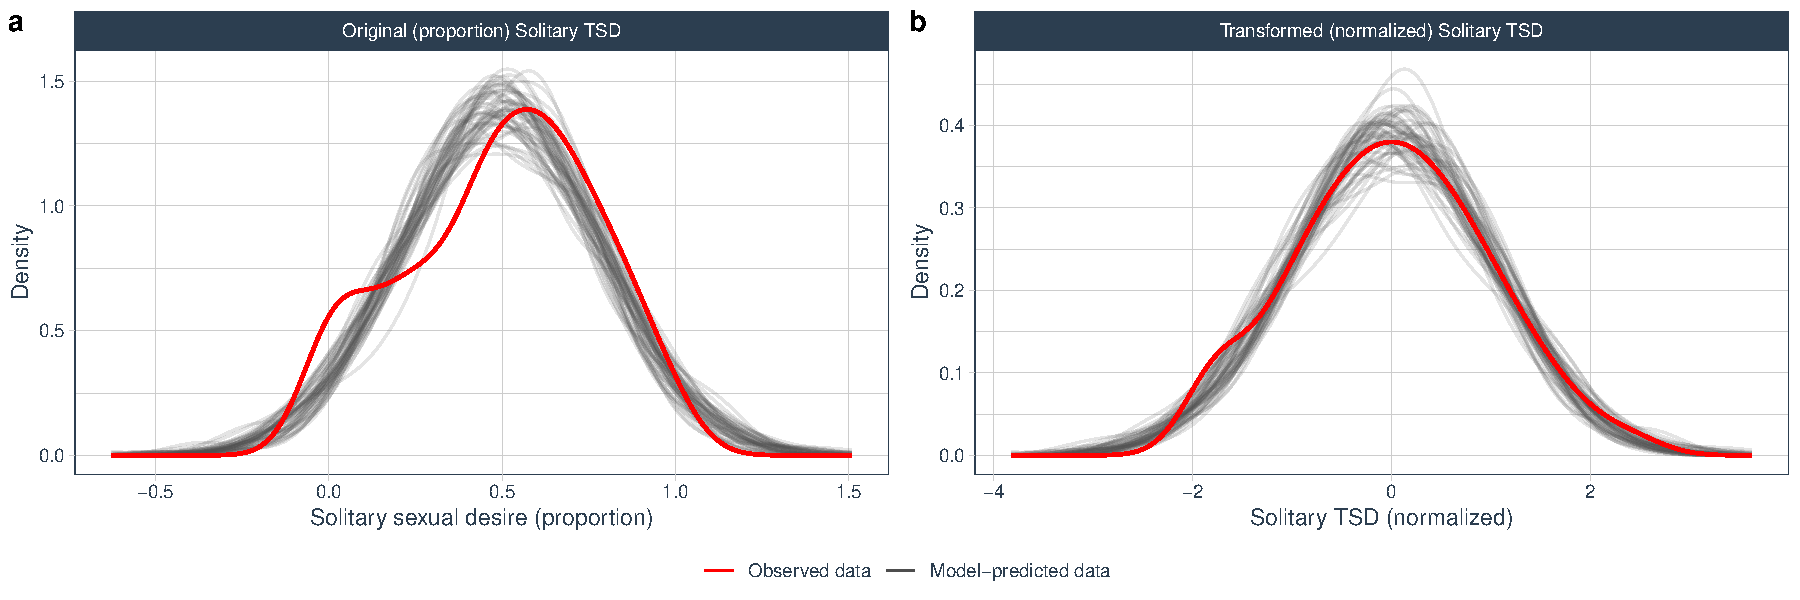
\includegraphics{Sexual_Desire_Arousal_anonymous_files/figure-latex/ppc-m1a-1.pdf}
\caption{\label{fig:ppc-m1a}Posterior predictive check. \textbf{(a)} Original (proportion) Solitary TSD; \textbf{(b)} Transformed (normalized) Solitary TSD. In both panels, red lines represent the observed data, and thin black lines represent 50 iterations of simulated data from each model.}
\end{figure}

\paragraph{\texorpdfstring{Table \ref{tab:tab-m1a}. ANOVA-type table for the interaction between \texttt{Relationship\ type}, and \texttt{Gender}}{Table \ref{tab:tab-m1a}. ANOVA-type table for the interaction between Relationship type, and Gender}}\label{table-reftabtab-m1a.-anova-type-table-for-the-interaction-between-relationship-type-and-gender}

This tables summarizes the results of the model.

\begin{Shaded}
\begin{Highlighting}[]
\CommentTok{\# Generate an ANOVA table summarizing the effects of Relationship Type and Gender on Solitary TSD}
\FunctionTok{anova.sig.lm}\NormalTok{(}
  \AttributeTok{model =}\NormalTok{ m1a\_norm,}
  \AttributeTok{custom\_caption =} \StringTok{"Effects of relationship type and gender on Solitary TSD"}
\NormalTok{)}
\end{Highlighting}
\end{Shaded}

\begin{table}[H]
\centering
\caption{\label{tab:tab-m1a}Effects of relationship type and gender on Solitary TSD}
\centering
\resizebox{\ifdim\width>\linewidth\linewidth\else\width\fi}{!}{
\begin{threeparttable}
\begin{tabular}[t]{lcccc}
\toprule
Effect & $df$ & $F$ & $p$ & $\epsilon^2_p$\\
\midrule
Gender & 1, 319 & 22.42 & \textbf{< 0.0001} & 0.06\\
Relationship & 1, 319 & 14.07 & \textbf{< 0.001} & 0.03\\
Gender × Relationship & 1, 319 & 4.23 & \textbf{0.04} & 0.01\\
\bottomrule
\end{tabular}
\begin{tablenotes}[para]
\item \textit{Note: } 
\item Sexual desire was transformed using an ordered quantile normalization (\cite{petersonOrderedQuantileNormalization2020a}). Results are Type III ANOVA. $R^2$ = 0.103, $R^2_{adjusted}$ = 0.095. Gender = participant's gender (women, men); Relationship = relationship type (stable, single). As effect size, we report partial epsilon squared ($\epsilon^2_p$), a less biased estimate than $\eta^2$ (see \cite{albersWhenPowerAnalyses2018}). Significant effects are in bold.
\end{tablenotes}
\end{threeparttable}}
\end{table}

\paragraph{\texorpdfstring{\emph{Post-hoc} comparisons}{Post-hoc comparisons}}\label{post-hoc-comparisons}

Because the main effects of gender, relationship type, and their interaction are significant, we explored these effects using estimated marginal means.

\subparagraph{Table \ref{tab:tab-m1a-emm1}. Estimated marginal means and contrasts between participants' gender.}\label{table-reftabtab-m1a-emm1.-estimated-marginal-means-and-contrasts-between-participants-gender.}

Table of estimated marginal means and contrasts between genders. All estimated marginal means and contrasts were calculated using the \texttt{emmeans} function from the \texttt{emmeans} package \autocite{emmeanscit}.

\begin{Shaded}
\begin{Highlighting}[]
\CommentTok{\# Compute estimated marginal means (EMMs) for Gender from the model}
\NormalTok{emms.m1a1 }\OtherTok{\textless{}{-}} \FunctionTok{emmeans}\NormalTok{(m1a\_norm, }\SpecialCharTok{\textasciitilde{}}\NormalTok{Gender)}

\CommentTok{\# Convert EMM results to a tibble for easier manipulation}
\NormalTok{emms.m1a1.tab }\OtherTok{\textless{}{-}} \FunctionTok{tibble}\NormalTok{(}\FunctionTok{data.frame}\NormalTok{(emms.m1a1))}

\CommentTok{\# Compute post{-}hoc contrasts and format p{-}values}
\NormalTok{t.m1a1 }\OtherTok{\textless{}{-}} \FunctionTok{contr.stars}\NormalTok{(emms.m1a1) }\SpecialCharTok{|\textgreater{}}
  \FunctionTok{mutate}\NormalTok{(}\AttributeTok{p.value =} \FunctionTok{pval.lev}\NormalTok{(p.value)) }\CommentTok{\# Format p{-}values for LaTeX}

\CommentTok{\# Merge EMM and contrast results, clean column names, and format output}
\FunctionTok{merge}\NormalTok{(emms.m1a1.tab, t.m1a1, }\AttributeTok{by =} \DecValTok{0}\NormalTok{, }\AttributeTok{all =} \ConstantTok{TRUE}\NormalTok{) }\SpecialCharTok{|\textgreater{}}
  \FunctionTok{select}\NormalTok{(}\SpecialCharTok{{-}}\FunctionTok{c}\NormalTok{(}\DecValTok{1}\NormalTok{, }\DecValTok{15}\NormalTok{)) }\SpecialCharTok{|\textgreater{}} \CommentTok{\# Remove unnecessary columns}
  \FunctionTok{unite}\NormalTok{(Contrast, group1, group2, }\AttributeTok{sep =} \StringTok{" {-} "}\NormalTok{) }\SpecialCharTok{|\textgreater{}} \CommentTok{\# Create contrast labels}
  \FunctionTok{mutate\_at}\NormalTok{(}\StringTok{"Contrast"}\NormalTok{, str\_replace\_all, }\StringTok{"NA {-} NA"}\NormalTok{, }\StringTok{" "}\NormalTok{) }\SpecialCharTok{|\textgreater{}} \CommentTok{\# Replace missing contrasts}
  \CommentTok{\# Create formatted table}
  \FunctionTok{kable}\NormalTok{(}
    \AttributeTok{digits =} \DecValTok{2}\NormalTok{, }\AttributeTok{booktabs =} \ConstantTok{TRUE}\NormalTok{, }\AttributeTok{align =} \FunctionTok{c}\NormalTok{(}\StringTok{"l"}\NormalTok{, }\FunctionTok{rep}\NormalTok{(}\StringTok{"c"}\NormalTok{, }\DecValTok{5}\NormalTok{), }\StringTok{"l"}\NormalTok{, }\FunctionTok{rep}\NormalTok{(}\StringTok{"c"}\NormalTok{, }\DecValTok{5}\NormalTok{)), }
    \AttributeTok{linesep =} \StringTok{""}\NormalTok{,}
    \AttributeTok{caption =} \StringTok{"Estimated marginal means and contrasts between participants\textquotesingle{} gender"}\NormalTok{, }
    \AttributeTok{escape =} \ConstantTok{FALSE}\NormalTok{,}
    \AttributeTok{col.names =} \FunctionTok{c}\NormalTok{(}
      \StringTok{"Gender"}\NormalTok{, }\StringTok{"EMM"}\NormalTok{, }\StringTok{"$SE$"}\NormalTok{, }\StringTok{"$df$"}\NormalTok{, }\StringTok{"$2.5}\SpecialCharTok{\textbackslash{}\textbackslash{}}\StringTok{\% CI$"}\NormalTok{, }\StringTok{"$97.5}\SpecialCharTok{\textbackslash{}\textbackslash{}}\StringTok{\% CI$"}\NormalTok{,}
      \StringTok{"Contrast"}\NormalTok{, }\StringTok{"Difference"}\NormalTok{, }\StringTok{"$SE$"}\NormalTok{, }\StringTok{"$df$"}\NormalTok{, }\StringTok{"$t$"}\NormalTok{, }\StringTok{"$p$"}
\NormalTok{    )}
\NormalTok{  ) }\SpecialCharTok{|\textgreater{}}
  \CommentTok{\# Add a header separating EMMs and contrasts}
  \FunctionTok{add\_header\_above}\NormalTok{(}\FunctionTok{c}\NormalTok{(}\StringTok{" "} \OtherTok{=} \DecValTok{6}\NormalTok{, }\StringTok{"Contrasts"} \OtherTok{=} \DecValTok{6}\NormalTok{)) }\SpecialCharTok{|\textgreater{}}
  \CommentTok{\# Apply LaTeX styling for table positioning}
  \FunctionTok{kable\_styling}\NormalTok{(}\AttributeTok{latex\_options =} \FunctionTok{c}\NormalTok{(}\StringTok{"HOLD\_position"}\NormalTok{, }\StringTok{"scale\_down"}\NormalTok{)) }\SpecialCharTok{|\textgreater{}}
  \CommentTok{\# Add footnote explaining significance formatting}
  \FunctionTok{footnote}\NormalTok{(}
    \AttributeTok{general =} \StringTok{"Significant effects are in bold."}\NormalTok{, }\AttributeTok{threeparttable =} \ConstantTok{TRUE}\NormalTok{,}
    \AttributeTok{footnote\_as\_chunk =} \ConstantTok{TRUE}\NormalTok{, }\AttributeTok{escape =} \ConstantTok{FALSE}
\NormalTok{  )}
\end{Highlighting}
\end{Shaded}

\begin{table}[H]
\centering
\caption{\label{tab:tab-m1a-emm1}Estimated marginal means and contrasts between participants' gender}
\centering
\resizebox{\ifdim\width>\linewidth\linewidth\else\width\fi}{!}{
\begin{threeparttable}
\begin{tabular}[t]{lccccclccccc}
\toprule
\multicolumn{6}{c}{ } & \multicolumn{6}{c}{Contrasts} \\
\cmidrule(l{3pt}r{3pt}){7-12}
Gender & EMM & $SE$ & $df$ & $2.5\% CI$ & $97.5\% CI$ & Contrast & Difference & $SE$ & $df$ & $t$ & $p$\\
\midrule
Women & -0.17 & 0.07 & 319 & -0.30 & -0.03 & Women - Men & -0.46 & 0.1 & 319 & -4.36 & \textbf{< 0.0001}\\
Men & 0.29 & 0.08 & 319 & 0.13 & 0.44 &  &  &  &  &  & \\
\bottomrule
\end{tabular}
\begin{tablenotes}[para]
\item \textit{Note: } 
\item Significant effects are in bold.
\end{tablenotes}
\end{threeparttable}}
\end{table}

\subparagraph{Table \ref{tab:tab-m1a-emm2}. Estimated marginal means and contrasts between relationship status.}\label{table-reftabtab-m1a-emm2.-estimated-marginal-means-and-contrasts-between-relationship-status.}

Table of estimated marginal means and contrasts between relationship status. All estimated marginal means and contrasts were calculated using the \texttt{emmeans} function from the \texttt{emmeans} package \autocite{emmeanscit}.

\begin{Shaded}
\begin{Highlighting}[]
\CommentTok{\# Compute estimated marginal means (EMMs) for Relationship Status from the model}
\NormalTok{emms.m1a2 }\OtherTok{\textless{}{-}} \FunctionTok{emmeans}\NormalTok{(m1a\_norm, }\SpecialCharTok{\textasciitilde{}}\NormalTok{Relationship)}

\CommentTok{\# Convert EMM results to a tibble for easier manipulation}
\NormalTok{emms.m1a2.tab }\OtherTok{\textless{}{-}} \FunctionTok{tibble}\NormalTok{(}\FunctionTok{data.frame}\NormalTok{(emms.m1a2))}

\CommentTok{\# Compute post{-}hoc contrasts and format p{-}values}
\NormalTok{t.m1a2 }\OtherTok{\textless{}{-}} \FunctionTok{contr.stars}\NormalTok{(emms.m1a2) }\SpecialCharTok{|\textgreater{}}
  \FunctionTok{mutate}\NormalTok{(}\AttributeTok{p.value =} \FunctionTok{pval.lev}\NormalTok{(p.value)) }\CommentTok{\# Format p{-}values for LaTeX}

\CommentTok{\# Merge EMM and contrast results, clean column names, and format output}
\FunctionTok{merge}\NormalTok{(emms.m1a2.tab, t.m1a2, }\AttributeTok{by =} \DecValTok{0}\NormalTok{, }\AttributeTok{all =} \ConstantTok{TRUE}\NormalTok{) }\SpecialCharTok{|\textgreater{}}
  \FunctionTok{select}\NormalTok{(}\SpecialCharTok{{-}}\FunctionTok{c}\NormalTok{(}\DecValTok{1}\NormalTok{, }\DecValTok{15}\NormalTok{)) }\SpecialCharTok{|\textgreater{}} \CommentTok{\# Remove unnecessary columns}
  \FunctionTok{unite}\NormalTok{(Contrast, group1, group2, }\AttributeTok{sep =} \StringTok{" {-} "}\NormalTok{) }\SpecialCharTok{|\textgreater{}} \CommentTok{\# Create contrast labels}
  \FunctionTok{mutate\_at}\NormalTok{(}\StringTok{"Contrast"}\NormalTok{, str\_replace\_all, }\StringTok{"NA {-} NA"}\NormalTok{, }\StringTok{" "}\NormalTok{) }\SpecialCharTok{|\textgreater{}} \CommentTok{\# Replace missing contrasts}
  \CommentTok{\# Create formatted table}
  \FunctionTok{kable}\NormalTok{(}
    \AttributeTok{digits =} \DecValTok{2}\NormalTok{, }\AttributeTok{booktabs =} \ConstantTok{TRUE}\NormalTok{, }\AttributeTok{align =} \FunctionTok{c}\NormalTok{(}\StringTok{"l"}\NormalTok{, }\FunctionTok{rep}\NormalTok{(}\StringTok{"c"}\NormalTok{, }\DecValTok{5}\NormalTok{), }\StringTok{"l"}\NormalTok{, }\FunctionTok{rep}\NormalTok{(}\StringTok{"c"}\NormalTok{, }\DecValTok{5}\NormalTok{)), }
    \AttributeTok{linesep =} \StringTok{""}\NormalTok{,}
    \AttributeTok{caption =} \StringTok{"Estimated marginal means and contrasts between relationship status"}\NormalTok{, }
    \AttributeTok{escape =} \ConstantTok{FALSE}\NormalTok{,}
    \AttributeTok{col.names =} \FunctionTok{c}\NormalTok{(}
      \StringTok{"Relationship type"}\NormalTok{, }\StringTok{"EMM"}\NormalTok{, }\StringTok{"$SE$"}\NormalTok{, }\StringTok{"$df$"}\NormalTok{, }\StringTok{"$2.5}\SpecialCharTok{\textbackslash{}\textbackslash{}}\StringTok{\% CI$"}\NormalTok{, }\StringTok{"$97.5}\SpecialCharTok{\textbackslash{}\textbackslash{}}\StringTok{\% CI$"}\NormalTok{,}
      \StringTok{"Contrast"}\NormalTok{, }\StringTok{"Difference"}\NormalTok{, }\StringTok{"$SE$"}\NormalTok{, }\StringTok{"$df$"}\NormalTok{, }\StringTok{"$t$"}\NormalTok{, }\StringTok{"$p$"}
\NormalTok{    )}
\NormalTok{  ) }\SpecialCharTok{|\textgreater{}}
  \CommentTok{\# Add a header separating EMMs and contrasts}
  \FunctionTok{add\_header\_above}\NormalTok{(}\FunctionTok{c}\NormalTok{(}\StringTok{" "} \OtherTok{=} \DecValTok{6}\NormalTok{, }\StringTok{"Contrasts"} \OtherTok{=} \DecValTok{6}\NormalTok{)) }\SpecialCharTok{|\textgreater{}}
  \CommentTok{\# Apply LaTeX styling for table positioning}
  \FunctionTok{kable\_styling}\NormalTok{(}\AttributeTok{latex\_options =} \FunctionTok{c}\NormalTok{(}\StringTok{"HOLD\_position"}\NormalTok{, }\StringTok{"scale\_down"}\NormalTok{)) }\SpecialCharTok{|\textgreater{}}
  \CommentTok{\# Add footnote explaining significance formatting}
  \FunctionTok{footnote}\NormalTok{(}
    \AttributeTok{general =} \StringTok{"Significant effects are in bold."}\NormalTok{, }\AttributeTok{threeparttable =} \ConstantTok{TRUE}\NormalTok{,}
    \AttributeTok{footnote\_as\_chunk =} \ConstantTok{TRUE}\NormalTok{, }\AttributeTok{escape =} \ConstantTok{FALSE}
\NormalTok{  )}
\end{Highlighting}
\end{Shaded}

\begin{table}[H]
\centering
\caption{\label{tab:tab-m1a-emm2}Estimated marginal means and contrasts between relationship status}
\centering
\resizebox{\ifdim\width>\linewidth\linewidth\else\width\fi}{!}{
\begin{threeparttable}
\begin{tabular}[t]{lccccclccccc}
\toprule
\multicolumn{6}{c}{ } & \multicolumn{6}{c}{Contrasts} \\
\cmidrule(l{3pt}r{3pt}){7-12}
Relationship type & EMM & $SE$ & $df$ & $2.5\% CI$ & $97.5\% CI$ & Contrast & Difference & $SE$ & $df$ & $t$ & $p$\\
\midrule
Stable & -0.09 & 0.07 & 319 & -0.23 & 0.05 & Stable - Single & -0.3 & 0.1 & 319 & -2.89 & \textbf{0.0041}\\
Single & 0.21 & 0.08 & 319 & 0.06 & 0.36 &  &  &  &  &  & \\
\bottomrule
\end{tabular}
\begin{tablenotes}[para]
\item \textit{Note: } 
\item Significant effects are in bold.
\end{tablenotes}
\end{threeparttable}}
\end{table}

\subparagraph{Table \ref{tab:tab-m1a-emm3}. Estimated marginal means and contrasts between gender by relationship status.}\label{table-reftabtab-m1a-emm3.-estimated-marginal-means-and-contrasts-between-gender-by-relationship-status.}

Table of estimated marginal means and contrasts between gender by relationship status. All estimated marginal means and contrasts were calculated using the \texttt{emmeans} function from the \texttt{emmeans} package \autocite{emmeanscit}.

\begin{Shaded}
\begin{Highlighting}[]
\CommentTok{\# Compute estimated marginal means (EMMs) for Gender within each Relationship Status}
\NormalTok{emms.m1a3 }\OtherTok{\textless{}{-}} \FunctionTok{emmeans}\NormalTok{(m1a\_norm, }\SpecialCharTok{\textasciitilde{}}\NormalTok{ Gender }\SpecialCharTok{|}\NormalTok{ Relationship)}

\CommentTok{\# Convert EMM results to a tibble for easier manipulation}
\NormalTok{emms.m1a3.tab }\OtherTok{\textless{}{-}} \FunctionTok{tibble}\NormalTok{(}\FunctionTok{data.frame}\NormalTok{(emms.m1a3))}

\CommentTok{\# Compute post{-}hoc contrasts and format p{-}values}
\NormalTok{t.m1a3 }\OtherTok{\textless{}{-}} \FunctionTok{contr.stars}\NormalTok{(emms.m1a3) }\SpecialCharTok{|\textgreater{}}
  \FunctionTok{mutate}\NormalTok{(}\AttributeTok{p.value =} \FunctionTok{pval.lev}\NormalTok{(p.value)) }\CommentTok{\# Format p{-}values for LaTeX}

\CommentTok{\# Insert NA rows to maintain table structure for grouped relationship status display}
\NormalTok{t.m1a3.f }\OtherTok{\textless{}{-}}\NormalTok{ t.m1a3 }\SpecialCharTok{|\textgreater{}}
  \FunctionTok{insertRows}\NormalTok{(}\DecValTok{2}\NormalTok{, }\AttributeTok{new =} \ConstantTok{NA}\NormalTok{) }\SpecialCharTok{|\textgreater{}} \CommentTok{\# Insert empty row after first contrast}
  \FunctionTok{insertRows}\NormalTok{(}\DecValTok{4}\NormalTok{, }\AttributeTok{new =} \ConstantTok{NA}\NormalTok{) }\CommentTok{\# Insert empty row after second contrast}

\CommentTok{\# Merge EMM and contrast results, clean column names, and format output}
\FunctionTok{merge}\NormalTok{(emms.m1a3.tab, t.m1a3.f, }\AttributeTok{by =} \DecValTok{0}\NormalTok{, }\AttributeTok{all =} \ConstantTok{TRUE}\NormalTok{) }\SpecialCharTok{|\textgreater{}}
  \FunctionTok{select}\NormalTok{(}\SpecialCharTok{{-}}\FunctionTok{c}\NormalTok{(}\DecValTok{1}\NormalTok{, }\DecValTok{3}\NormalTok{, }\DecValTok{11}\NormalTok{, }\DecValTok{17}\NormalTok{)) }\SpecialCharTok{|\textgreater{}} \CommentTok{\# Remove unnecessary columns}
  \FunctionTok{drop\_na}\NormalTok{(Gender) }\SpecialCharTok{|\textgreater{}} \CommentTok{\# Ensure Gender column is complete}
  \FunctionTok{unite}\NormalTok{(Contrast, group1, group2, }\AttributeTok{sep =} \StringTok{" {-} "}\NormalTok{) }\SpecialCharTok{|\textgreater{}} \CommentTok{\# Create contrast labels}
  \FunctionTok{mutate\_at}\NormalTok{(}\StringTok{"Contrast"}\NormalTok{, str\_replace\_all, }\StringTok{"NA {-} NA"}\NormalTok{, }\StringTok{""}\NormalTok{) }\SpecialCharTok{|\textgreater{}} \CommentTok{\# Replace missing contrasts}
  \CommentTok{\# Create formatted table}
  \FunctionTok{kable}\NormalTok{(}
    \AttributeTok{digits =} \DecValTok{2}\NormalTok{, }\AttributeTok{booktabs =} \ConstantTok{TRUE}\NormalTok{, }\AttributeTok{align =} \FunctionTok{c}\NormalTok{(}\StringTok{"l"}\NormalTok{, }\StringTok{"l"}\NormalTok{, }\FunctionTok{rep}\NormalTok{(}\StringTok{"c"}\NormalTok{, }\DecValTok{5}\NormalTok{), }\StringTok{"l"}\NormalTok{, }\FunctionTok{rep}\NormalTok{(}\StringTok{"c"}\NormalTok{, }\DecValTok{5}\NormalTok{)), }
    \AttributeTok{linesep =} \StringTok{""}\NormalTok{,}
    \AttributeTok{caption =} \StringTok{"Estimated marginal means and contrasts between gender by relationship status"}\NormalTok{,}
    \AttributeTok{escape =} \ConstantTok{FALSE}\NormalTok{,}
    \AttributeTok{col.names =} \FunctionTok{c}\NormalTok{(}
      \StringTok{"Gender"}\NormalTok{, }\StringTok{"EMM"}\NormalTok{, }\StringTok{"$SE$"}\NormalTok{, }\StringTok{"$df$"}\NormalTok{, }\StringTok{"$2.5}\SpecialCharTok{\textbackslash{}\textbackslash{}}\StringTok{\% CI$"}\NormalTok{, }\StringTok{"$97.5}\SpecialCharTok{\textbackslash{}\textbackslash{}}\StringTok{\% CI$"}\NormalTok{,}
      \StringTok{"Contrast"}\NormalTok{, }\StringTok{"Difference"}\NormalTok{, }\StringTok{"$SE$"}\NormalTok{, }\StringTok{"$df$"}\NormalTok{, }\StringTok{"$t$"}\NormalTok{, }\StringTok{"$p$"}
\NormalTok{    )}
\NormalTok{  ) }\SpecialCharTok{|\textgreater{}}
  \CommentTok{\# Add grouped row labels for Relationship Status}
  \FunctionTok{pack\_rows}\NormalTok{(}\StringTok{"Relationship status: Stable"}\NormalTok{,}
    \AttributeTok{start\_row =} \DecValTok{1}\NormalTok{, }\AttributeTok{end\_row =} \DecValTok{2}\NormalTok{,}
    \AttributeTok{bold =} \ConstantTok{FALSE}\NormalTok{, }\AttributeTok{background =} \StringTok{"lightgray"}
\NormalTok{  ) }\SpecialCharTok{|\textgreater{}}
  \FunctionTok{pack\_rows}\NormalTok{(}\StringTok{"Relationship status: Single"}\NormalTok{,}
    \AttributeTok{start\_row =} \DecValTok{3}\NormalTok{, }\AttributeTok{end\_row =} \DecValTok{4}\NormalTok{,}
    \AttributeTok{bold =} \ConstantTok{FALSE}\NormalTok{, }\AttributeTok{background =} \StringTok{"lightgray"}
\NormalTok{  ) }\SpecialCharTok{|\textgreater{}}
  \CommentTok{\# Add a header separating EMMs and contrasts}
  \FunctionTok{add\_header\_above}\NormalTok{(}\FunctionTok{c}\NormalTok{(}\StringTok{" "} \OtherTok{=} \DecValTok{6}\NormalTok{, }\StringTok{"Contrasts"} \OtherTok{=} \DecValTok{6}\NormalTok{)) }\SpecialCharTok{|\textgreater{}}
  \CommentTok{\# Apply LaTeX styling for table positioning}
  \FunctionTok{kable\_styling}\NormalTok{(}\AttributeTok{latex\_options =} \FunctionTok{c}\NormalTok{(}\StringTok{"HOLD\_position"}\NormalTok{, }\StringTok{"scale\_down"}\NormalTok{)) }\SpecialCharTok{|\textgreater{}}
  \CommentTok{\# Add footnote explaining significance formatting}
  \FunctionTok{footnote}\NormalTok{(}
    \AttributeTok{general =} \StringTok{"Significant effects are in bold."}\NormalTok{, }\AttributeTok{threeparttable =} \ConstantTok{TRUE}\NormalTok{,}
    \AttributeTok{footnote\_as\_chunk =} \ConstantTok{TRUE}\NormalTok{, }\AttributeTok{escape =} \ConstantTok{FALSE}
\NormalTok{  )}
\end{Highlighting}
\end{Shaded}

\begin{table}[H]
\centering
\caption{\label{tab:tab-m1a-emm3}Estimated marginal means and contrasts between gender by relationship status}
\centering
\resizebox{\ifdim\width>\linewidth\linewidth\else\width\fi}{!}{
\begin{threeparttable}
\begin{tabular}[t]{llccccclcccc}
\toprule
\multicolumn{6}{c}{ } & \multicolumn{6}{c}{Contrasts} \\
\cmidrule(l{3pt}r{3pt}){7-12}
Gender & EMM & $SE$ & $df$ & $2.5\% CI$ & $97.5\% CI$ & Contrast & Difference & $SE$ & $df$ & $t$ & $p$\\
\midrule
\addlinespace[0.3em]
\multicolumn{12}{l}{\cellcolor{lightgray}{Relationship status: Stable}}\\
\hspace{1em}Women & -0.43 & 0.09 & 319 & -0.61 & -0.25 & Women - Men & -0.67 & 0.14 & 319 & -4.74 & \textbf{< 0.0001}\\
\hspace{1em}Men & 0.24 & 0.11 & 319 & 0.03 & 0.46 &  &  &  &  &  & \\
\addlinespace[0.3em]
\multicolumn{12}{l}{\cellcolor{lightgray}{Relationship status: Single}}\\
\hspace{1em}Women & 0.09 & 0.10 & 319 & -0.11 & 0.30 & Women - Men & -0.24 & 0.15 & 319 & -1.57 & 0.12\\
\hspace{1em}Men & 0.33 & 0.11 & 319 & 0.11 & 0.55 &  &  &  &  &  & \\
\bottomrule
\end{tabular}
\begin{tablenotes}[para]
\item \textit{Note: } 
\item Significant effects are in bold.
\end{tablenotes}
\end{threeparttable}}
\end{table}

\paragraph{Figure \ref{fig:fig-h1a}. Effects of gender and relationship type on Solitary TSD}\label{figure-reffigfig-h1a.-effects-of-gender-and-relationship-type-on-solitary-tsd}

This figure summarizes the results of hypothesis 1a.

\begin{Shaded}
\begin{Highlighting}[]
\CommentTok{\# Plot (a): Main effect of Gender on Solitary TSD}
\NormalTok{h1a1 }\OtherTok{\textless{}{-}} \FunctionTok{ggplot}\NormalTok{(dat\_m1, }\FunctionTok{aes}\NormalTok{(}
  \AttributeTok{x =}\NormalTok{ Gender, }\AttributeTok{y =} \StringTok{\textasciigrave{}}\AttributeTok{Solitary TSD (normalized)}\StringTok{\textasciigrave{}}\NormalTok{, }\AttributeTok{color =}\NormalTok{ Gender}
\NormalTok{)) }\SpecialCharTok{+}
  \FunctionTok{scale\_color\_manual}\NormalTok{(}\AttributeTok{values =}\NormalTok{ color.Gender) }\SpecialCharTok{+}
  \FunctionTok{scale\_fill\_manual}\NormalTok{(}\AttributeTok{values =}\NormalTok{ color.Gender) }\SpecialCharTok{+}
  \FunctionTok{geom\_linerange}\NormalTok{(}
    \AttributeTok{data =}\NormalTok{ emms.m1a1.tab }\SpecialCharTok{|\textgreater{}} \FunctionTok{rename}\NormalTok{(}\StringTok{"Solitary TSD (normalized)"} \OtherTok{=}\NormalTok{ emmean),}
    \AttributeTok{mapping =} \FunctionTok{aes}\NormalTok{(}\AttributeTok{ymin =}\NormalTok{ lower.CL, }\AttributeTok{ymax =}\NormalTok{ upper.CL)}
\NormalTok{  ) }\SpecialCharTok{+}
  \FunctionTok{geom\_point}\NormalTok{(}
    \AttributeTok{data =}\NormalTok{ emms.m1a1.tab }\SpecialCharTok{|\textgreater{}} \FunctionTok{rename}\NormalTok{(}\StringTok{"Solitary TSD (normalized)"} \OtherTok{=}\NormalTok{ emmean),}
    \AttributeTok{position =} \FunctionTok{position\_dodge}\NormalTok{(}\FloatTok{0.1}\NormalTok{), }\AttributeTok{size =} \DecValTok{3}
\NormalTok{  ) }\SpecialCharTok{+}
  \FunctionTok{stat\_pvalue\_manual}\NormalTok{(t.m1a1, }\AttributeTok{label =} \StringTok{"p.signif"}\NormalTok{, }\AttributeTok{y.position =} \FloatTok{0.55}\NormalTok{, }\AttributeTok{tip.length =} \DecValTok{0}\NormalTok{) }\SpecialCharTok{+}
  \FunctionTok{guides}\NormalTok{(}\AttributeTok{color =} \StringTok{"none"}\NormalTok{) }\SpecialCharTok{+}
  \FunctionTok{theme\_tq}\NormalTok{()}

\CommentTok{\# Plot (b): Main effect of Relationship on Solitary TSD}
\NormalTok{h1a2 }\OtherTok{\textless{}{-}} \FunctionTok{ggplot}\NormalTok{(dat\_m1, }\FunctionTok{aes}\NormalTok{(}
  \AttributeTok{x =}\NormalTok{ Relationship, }\AttributeTok{y =} \StringTok{\textasciigrave{}}\AttributeTok{Solitary TSD (normalized)}\StringTok{\textasciigrave{}}\NormalTok{, }\AttributeTok{color =}\NormalTok{ Relationship}
\NormalTok{)) }\SpecialCharTok{+}
  \FunctionTok{scale\_color\_manual}\NormalTok{(}\AttributeTok{values =}\NormalTok{ color.Relationship) }\SpecialCharTok{+}
  \FunctionTok{scale\_fill\_manual}\NormalTok{(}\AttributeTok{values =}\NormalTok{ color.Relationship) }\SpecialCharTok{+}
  \FunctionTok{geom\_linerange}\NormalTok{(}
    \AttributeTok{data =}\NormalTok{ emms.m1a2.tab }\SpecialCharTok{|\textgreater{}} \FunctionTok{rename}\NormalTok{(}\StringTok{"Solitary TSD (normalized)"} \OtherTok{=}\NormalTok{ emmean),}
    \AttributeTok{mapping =} \FunctionTok{aes}\NormalTok{(}\AttributeTok{ymin =}\NormalTok{ lower.CL, }\AttributeTok{ymax =}\NormalTok{ upper.CL)}
\NormalTok{  ) }\SpecialCharTok{+}
  \FunctionTok{geom\_point}\NormalTok{(}
    \AttributeTok{data =}\NormalTok{ emms.m1a2.tab }\SpecialCharTok{|\textgreater{}} \FunctionTok{rename}\NormalTok{(}\StringTok{"Solitary TSD (normalized)"} \OtherTok{=}\NormalTok{ emmean),}
    \AttributeTok{position =} \FunctionTok{position\_dodge}\NormalTok{(}\FloatTok{0.1}\NormalTok{), }\AttributeTok{size =} \DecValTok{3}
\NormalTok{  ) }\SpecialCharTok{+}
  \FunctionTok{stat\_pvalue\_manual}\NormalTok{(t.m1a2, }\AttributeTok{label =} \StringTok{"p.signif"}\NormalTok{, }\AttributeTok{y.position =} \FloatTok{0.45}\NormalTok{, }\AttributeTok{tip.length =} \DecValTok{0}\NormalTok{) }\SpecialCharTok{+}
  \FunctionTok{guides}\NormalTok{(}\AttributeTok{color =} \StringTok{"none"}\NormalTok{) }\SpecialCharTok{+}
  \FunctionTok{theme\_tq}\NormalTok{()}

\CommentTok{\# Plot (c): Gender × Relationship Interaction on Solitary TSD}
\NormalTok{h1a3 }\OtherTok{\textless{}{-}} \FunctionTok{ggplot}\NormalTok{(dat\_m1, }\FunctionTok{aes}\NormalTok{(}
  \AttributeTok{x =}\NormalTok{ Gender, }\AttributeTok{y =} \StringTok{\textasciigrave{}}\AttributeTok{Solitary TSD (normalized)}\StringTok{\textasciigrave{}}\NormalTok{, }\AttributeTok{color =}\NormalTok{ Gender}
\NormalTok{)) }\SpecialCharTok{+}
  \FunctionTok{scale\_color\_manual}\NormalTok{(}\AttributeTok{values =}\NormalTok{ color.Gender) }\SpecialCharTok{+}
  \FunctionTok{scale\_fill\_manual}\NormalTok{(}\AttributeTok{values =}\NormalTok{ color.Gender) }\SpecialCharTok{+}
  \FunctionTok{facet\_wrap}\NormalTok{(}\SpecialCharTok{\textasciitilde{}}\NormalTok{Relationship) }\SpecialCharTok{+}
  \FunctionTok{geom\_linerange}\NormalTok{(}
    \AttributeTok{data =}\NormalTok{ emms.m1a3.tab }\SpecialCharTok{|\textgreater{}} \FunctionTok{rename}\NormalTok{(}\StringTok{"Solitary TSD (normalized)"} \OtherTok{=}\NormalTok{ emmean),}
    \AttributeTok{mapping =} \FunctionTok{aes}\NormalTok{(}\AttributeTok{ymin =}\NormalTok{ lower.CL, }\AttributeTok{ymax =}\NormalTok{ upper.CL)}
\NormalTok{  ) }\SpecialCharTok{+}
  \FunctionTok{geom\_point}\NormalTok{(}
    \AttributeTok{data =}\NormalTok{ emms.m1a3.tab }\SpecialCharTok{|\textgreater{}} \FunctionTok{rename}\NormalTok{(}\StringTok{"Solitary TSD (normalized)"} \OtherTok{=}\NormalTok{ emmean),}
    \AttributeTok{position =} \FunctionTok{position\_dodge}\NormalTok{(}\FloatTok{0.1}\NormalTok{), }\AttributeTok{size =} \DecValTok{3}
\NormalTok{  ) }\SpecialCharTok{+}
  \FunctionTok{stat\_pvalue\_manual}\NormalTok{(t.m1a3, }\AttributeTok{label =} \StringTok{"p.signif"}\NormalTok{, }\AttributeTok{y.position =} \FloatTok{0.7}\NormalTok{, }\AttributeTok{tip.length =} \DecValTok{0}\NormalTok{) }\SpecialCharTok{+}
  \FunctionTok{guides}\NormalTok{(}\AttributeTok{color =} \StringTok{"none"}\NormalTok{) }\SpecialCharTok{+}
  \FunctionTok{theme\_tq}\NormalTok{()}

\CommentTok{\# Combine the three plots into a single figure}
\NormalTok{p1a }\OtherTok{\textless{}{-}} \FunctionTok{ggarrange}\NormalTok{(h1a1, h1a2 }\SpecialCharTok{+} \FunctionTok{labs}\NormalTok{(}\AttributeTok{y =} \ConstantTok{NULL}\NormalTok{), h1a3 }\SpecialCharTok{+} \FunctionTok{labs}\NormalTok{(}\AttributeTok{y =} \ConstantTok{NULL}\NormalTok{),}
  \AttributeTok{ncol =} \DecValTok{3}\NormalTok{, }\AttributeTok{labels =} \StringTok{"auto"}\NormalTok{, }\AttributeTok{widths =} \FunctionTok{c}\NormalTok{(}\DecValTok{1}\NormalTok{, }\DecValTok{1}\NormalTok{, }\FloatTok{1.5}\NormalTok{) }\CommentTok{\# Adjust widths for better alignment}
\NormalTok{)}

\CommentTok{\# Display the final figure}
\NormalTok{p1a}
\end{Highlighting}
\end{Shaded}

\begin{figure}
\centering
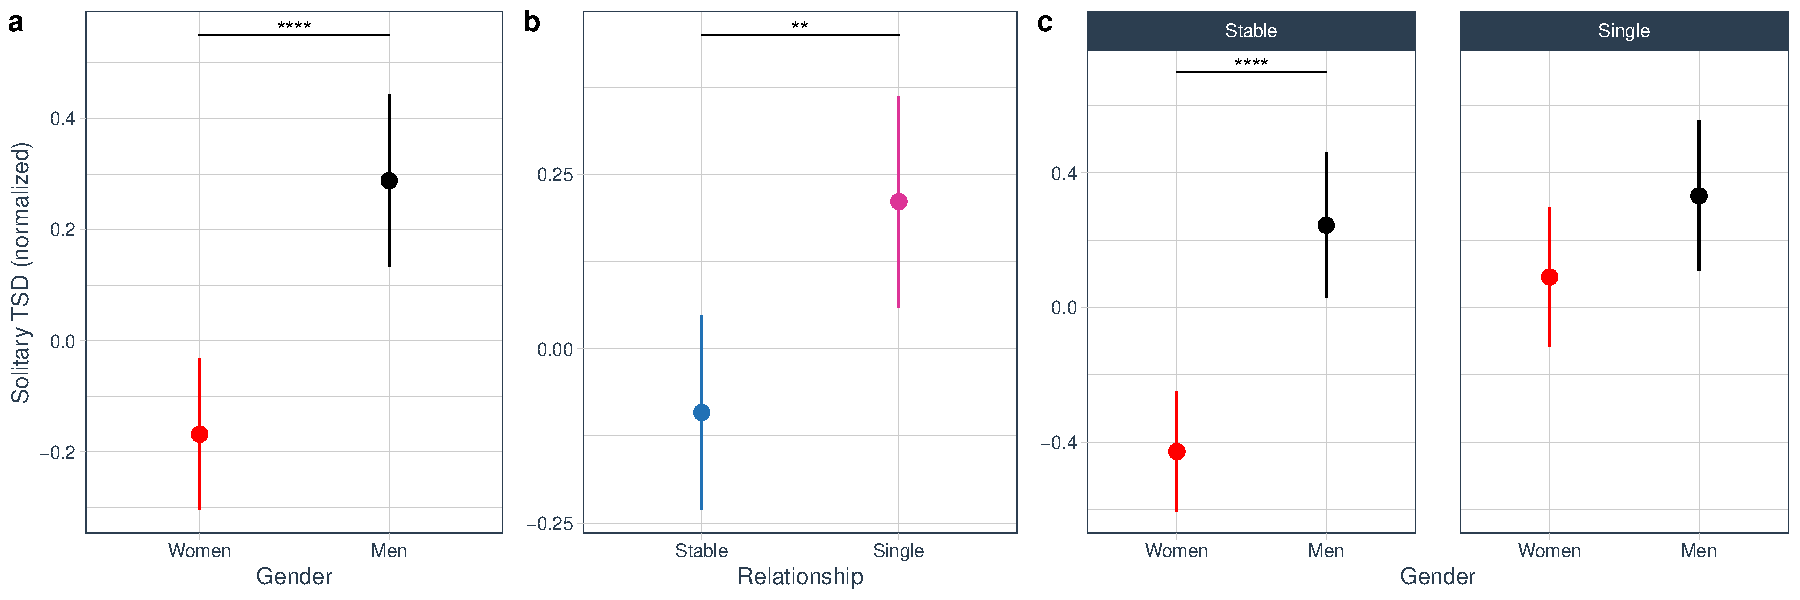
\includegraphics{Sexual_Desire_Arousal_anonymous_files/figure-latex/fig-h1a-1.pdf}
\caption{\label{fig:fig-h1a}Effects of gender and relationship type on Solitary TSD. Solitary sexual desire was transformed using ordered quantile normalization \autocite{petersonOrderedQuantileNormalization2020a}. \textbf{(a)} Simple comparison between sexual desire by gender (for detailed results, see Table \ref{tab:tab-m1a-emm1}); \textbf{(b)} Simple comparison between relationship status levels (for detailed results, see Table \ref{tab:tab-m1a-emm2}); \textbf{(c)} Interaction between relationship type and relationship status (see Table \ref{tab:tab-m1a}; for detailed results, see Table \ref{tab:tab-m1a-emm3}). Dots and bars represent estimated marginal means and 95\% CI. In all cases, significant effects are represented with lines and stars: *\emph{p} \textless{} 0.05, **\emph{p} \textless{} 0.01, ***\emph{p} \textless{} 0.001, ****\emph{p} \textless{} 0.0001.}
\end{figure}

\subsubsection{Hypothesis 1b: Dyadic TSD (Attractive person)}\label{hypothesis1b}

\paragraph{Model the effects of relationship type and gender on Dyadic TSD: Attractive person}\label{model-the-effects-of-relationship-type-and-gender-on-dyadic-tsd-attractive-person}

We fitted models with both the original (proportion; \texttt{m1b\_prop}) and transformed (normalized; \texttt{m1b\_norm}) TSD scores, and performed posterior predictive checks (PPCs). As shown elsewhere \autocite[e.g.,][]{gabryVisualizationBayesianWorkflow2019}, if simulated data from one model are more similar to the observed outcome, that model is likely to be preferred.

\begin{Shaded}
\begin{Highlighting}[]
\CommentTok{\# Set contrast options for sum coding (useful for ANOVA{-}like interpretation)}
\FunctionTok{options}\NormalTok{(}\AttributeTok{contrasts =} \FunctionTok{c}\NormalTok{(}\StringTok{"contr.sum"}\NormalTok{, }\StringTok{"contr.poly"}\NormalTok{))}

\CommentTok{\# Fit a linear model using the original proportion{-}based Dyadic TSD (Attractive Person) scores}
\NormalTok{m1b\_prop }\OtherTok{\textless{}{-}} \FunctionTok{lm}\NormalTok{(}
  \StringTok{\textasciigrave{}}\AttributeTok{Dyadic TSD Attractive Person (proportion)}\StringTok{\textasciigrave{}} \SpecialCharTok{\textasciitilde{}}\NormalTok{ Gender }\SpecialCharTok{*}\NormalTok{ Relationship,}
  \AttributeTok{data =}\NormalTok{ dat\_m1}
\NormalTok{)}

\CommentTok{\# Fit a linear model using the normalized Dyadic TSD (Attractive Person) scores}
\NormalTok{m1b\_norm }\OtherTok{\textless{}{-}} \FunctionTok{lm}\NormalTok{(}
  \StringTok{\textasciigrave{}}\AttributeTok{Dyadic TSD Attractive Person (normalized)}\StringTok{\textasciigrave{}} \SpecialCharTok{\textasciitilde{}}\NormalTok{ Gender }\SpecialCharTok{*}\NormalTok{ Relationship,}
  \AttributeTok{data =}\NormalTok{ dat\_m1}
\NormalTok{)}
\end{Highlighting}
\end{Shaded}

\subparagraph{Figure \ref{fig:ppc-m1b}: Posterior predictive checks (PPCs) for Hypothesis 1b.}\label{figure-reffigppc-m1b-posterior-predictive-checks-ppcs-for-hypothesis-1b.}

PPCs were performed using the \texttt{check\_model} function from the \texttt{performance} package \autocite{ludecke2021}, and reported in Fig. \ref{fig:ppc-m1b}. Simulated data from the normalized Solitary TSD model (Fig. \ref{fig:ppc-m1b}b) are more similar to the observed outcome, so this model is preferred.

\begin{Shaded}
\begin{Highlighting}[]
\CommentTok{\# Perform posterior predictive checks (PPC) and arrange them into a single figure}
\NormalTok{ppc\_m1b }\OtherTok{\textless{}{-}} \FunctionTok{ggarrange}\NormalTok{(}
  \CommentTok{\# PPC plot for the original (proportion) Dyadic TSD: Attractive Person model}
  \FunctionTok{plot}\NormalTok{(}
    \FunctionTok{check\_model}\NormalTok{(m1b\_prop, }\AttributeTok{panel =} \ConstantTok{FALSE}\NormalTok{, }\AttributeTok{check =} \StringTok{"pp\_check"}\NormalTok{)}\SpecialCharTok{$}\NormalTok{PP\_CHECK,}
    \AttributeTok{colors =} \FunctionTok{c}\NormalTok{(}\StringTok{"red"}\NormalTok{, }\StringTok{"grey30"}\NormalTok{) }\CommentTok{\# Red for observed data, grey for simulated data}
\NormalTok{  ) }\SpecialCharTok{+}
    \FunctionTok{labs}\NormalTok{(}\AttributeTok{title =} \ConstantTok{NULL}\NormalTok{, }\AttributeTok{subtitle =} \ConstantTok{NULL}\NormalTok{) }\SpecialCharTok{+}
    \FunctionTok{theme\_tq}\NormalTok{() }\SpecialCharTok{+}
    \FunctionTok{facet\_wrap}\NormalTok{(}\SpecialCharTok{\textasciitilde{}}\DecValTok{1}\NormalTok{, }\AttributeTok{labeller =} \FunctionTok{as\_labeller}\NormalTok{(}\FunctionTok{c}\NormalTok{(}
      \StringTok{"1"} \OtherTok{=} \StringTok{"Original (proportion) Dyadic TSD: Attractive person"}
\NormalTok{    ))),}
  \CommentTok{\# PPC plot for the transformed (normalized) Dyadic TSD: Attractive Person model}
  \FunctionTok{plot}\NormalTok{(}
    \FunctionTok{check\_model}\NormalTok{(m1b\_norm, }\AttributeTok{panel =} \ConstantTok{FALSE}\NormalTok{, }\AttributeTok{check =} \StringTok{"pp\_check"}\NormalTok{)}\SpecialCharTok{$}\NormalTok{PP\_CHECK,}
    \AttributeTok{colors =} \FunctionTok{c}\NormalTok{(}\StringTok{"red"}\NormalTok{, }\StringTok{"grey30"}\NormalTok{)}
\NormalTok{  ) }\SpecialCharTok{+}
    \FunctionTok{labs}\NormalTok{(}\AttributeTok{title =} \ConstantTok{NULL}\NormalTok{, }\AttributeTok{subtitle =} \ConstantTok{NULL}\NormalTok{) }\SpecialCharTok{+}
    \FunctionTok{theme\_tq}\NormalTok{() }\SpecialCharTok{+}
    \FunctionTok{facet\_wrap}\NormalTok{(}\SpecialCharTok{\textasciitilde{}}\DecValTok{1}\NormalTok{, }\AttributeTok{labeller =} \FunctionTok{as\_labeller}\NormalTok{(}\FunctionTok{c}\NormalTok{(}
      \StringTok{"1"} \OtherTok{=} \StringTok{"Transformed (normalized) Dyadic TSD: Attractive person"}
\NormalTok{    ))),}
  \AttributeTok{labels =} \StringTok{"auto"}\NormalTok{, }\CommentTok{\# Automatically label subplots (a, b)}
  \AttributeTok{common.legend =} \ConstantTok{TRUE}\NormalTok{, }\AttributeTok{legend =} \StringTok{"bottom"} \CommentTok{\# Use a common legend at the bottom}
\NormalTok{)}

\CommentTok{\# Display the final PPC figure}
\NormalTok{ppc\_m1b}
\end{Highlighting}
\end{Shaded}

\begin{figure}
\centering
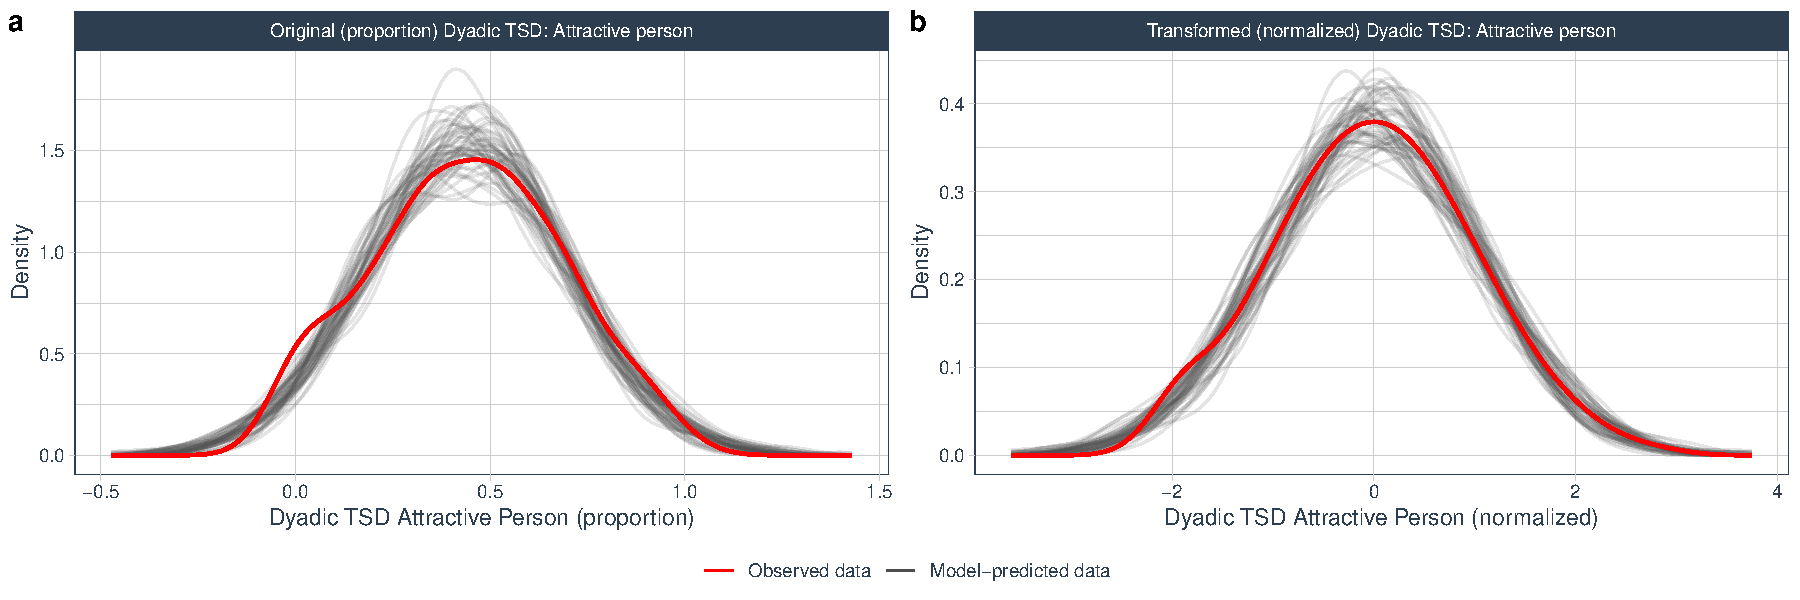
\includegraphics{Sexual_Desire_Arousal_anonymous_files/figure-latex/ppc-m1b-1.pdf}
\caption{\label{fig:ppc-m1b}Posterior predictive check. \textbf{(a)} Original (proportion) Solitary TSD; \textbf{(b)} Transformed (normalized) Solitary TSD. In both panels, red lines represent the observed data, and thin black lines represent 50 iterations of simulated data from each model.}
\end{figure}

\paragraph{\texorpdfstring{Table \ref{tab:tab-m1b}. ANOVA-type table for the interaction between \texttt{Relationship\ type}, and \texttt{Gender}}{Table \ref{tab:tab-m1b}. ANOVA-type table for the interaction between Relationship type, and Gender}}\label{table-reftabtab-m1b.-anova-type-table-for-the-interaction-between-relationship-type-and-gender}

This tables summarizes the results of the model.

\begin{Shaded}
\begin{Highlighting}[]
\CommentTok{\# Generate an ANOVA table summarizing the effects of Relationship Type and Gender on}
\CommentTok{\# Dyadic TSD Attractive Person}
\FunctionTok{anova.sig.lm}\NormalTok{(}
  \AttributeTok{model =}\NormalTok{ m1b\_norm,}
  \AttributeTok{custom\_caption =} \StringTok{"Effects of relationship type and gender on Dyadic TSD Attractive Person"}
\NormalTok{)}
\end{Highlighting}
\end{Shaded}

\begin{table}[H]
\centering
\caption{\label{tab:tab-m1b}Effects of relationship type and gender on Dyadic TSD Attractive Person}
\centering
\resizebox{\ifdim\width>\linewidth\linewidth\else\width\fi}{!}{
\begin{threeparttable}
\begin{tabular}[t]{lcccc}
\toprule
Effect & $df$ & $F$ & $p$ & $\epsilon^2_p$\\
\midrule
Gender & 1, 319 & 29.85 & \textbf{< 0.0001} & 0.09\\
Relationship & 1, 319 & 8.20 & \textbf{0.004} & 0.03\\
Gender × Relationship & 1, 319 & 1.73 & 0.19 & 0.00\\
\bottomrule
\end{tabular}
\begin{tablenotes}[para]
\item \textit{Note: } 
\item Sexual desire was transformed using an ordered quantile normalization (\cite{petersonOrderedQuantileNormalization2020a}). Results are Type III ANOVA. $R^2$ = 0.122, $R^2_{adjusted}$ = 0.114. Gender = participant's gender (women, men); Relationship = relationship type (stable, single). As effect size, we report partial epsilon squared ($\epsilon^2_p$), a less biased estimate than $\eta^2$ (see \cite{albersWhenPowerAnalyses2018}). Significant effects are in bold.
\end{tablenotes}
\end{threeparttable}}
\end{table}

\paragraph{\texorpdfstring{\emph{Post-hoc} comparisons}{Post-hoc comparisons}}\label{post-hoc-comparisons-1}

Because the main effects of gender and relationship type, but not their interaction, are significant, we explored these effects using estimated marginal means.

\subparagraph{Table \ref{tab:tab-m1b-emm1}. Estimated marginal means and contrasts between participants' gender.}\label{table-reftabtab-m1b-emm1.-estimated-marginal-means-and-contrasts-between-participants-gender.}

Table of estimated marginal means and contrasts between genders. All estimated marginal means and contrasts were calculated using the \texttt{emmeans} function from the \texttt{emmeans} package \autocite{emmeanscit}.

\begin{Shaded}
\begin{Highlighting}[]
\CommentTok{\# Compute estimated marginal means (EMMs) for Gender from the model}
\NormalTok{emms.m1b1 }\OtherTok{\textless{}{-}} \FunctionTok{emmeans}\NormalTok{(m1b\_norm, }\SpecialCharTok{\textasciitilde{}}\NormalTok{Gender)}

\CommentTok{\# Convert EMM results to a tibble for easier manipulation}
\NormalTok{emms.m1b1.tab }\OtherTok{\textless{}{-}} \FunctionTok{tibble}\NormalTok{(}\FunctionTok{data.frame}\NormalTok{(emms.m1b1))}

\CommentTok{\# Compute post{-}hoc contrasts and format p{-}values}
\NormalTok{t.m1b1 }\OtherTok{\textless{}{-}} \FunctionTok{contr.stars}\NormalTok{(emms.m1b1) }\SpecialCharTok{|\textgreater{}}
  \FunctionTok{mutate}\NormalTok{(}\AttributeTok{p.value =} \FunctionTok{pval.lev}\NormalTok{(p.value)) }\CommentTok{\# Format p{-}values for LaTeX}

\CommentTok{\# Merge EMM and contrast results, clean column names, and format output}
\FunctionTok{merge}\NormalTok{(emms.m1b1.tab, t.m1b1, }\AttributeTok{by =} \DecValTok{0}\NormalTok{, }\AttributeTok{all =} \ConstantTok{TRUE}\NormalTok{) }\SpecialCharTok{|\textgreater{}}
  \FunctionTok{select}\NormalTok{(}\SpecialCharTok{{-}}\FunctionTok{c}\NormalTok{(}\DecValTok{1}\NormalTok{, }\DecValTok{15}\NormalTok{)) }\SpecialCharTok{|\textgreater{}} \CommentTok{\# Remove unnecessary columns}
  \FunctionTok{unite}\NormalTok{(Contrast, group1, group2, }\AttributeTok{sep =} \StringTok{" {-} "}\NormalTok{) }\SpecialCharTok{|\textgreater{}} \CommentTok{\# Create contrast labels}
  \FunctionTok{mutate\_at}\NormalTok{(}\StringTok{"Contrast"}\NormalTok{, str\_replace\_all, }\StringTok{"NA {-} NA"}\NormalTok{, }\StringTok{" "}\NormalTok{) }\SpecialCharTok{|\textgreater{}} \CommentTok{\# Replace missing contrasts}
  \CommentTok{\# Create formatted table}
  \FunctionTok{kable}\NormalTok{(}
    \AttributeTok{digits =} \DecValTok{2}\NormalTok{, }\AttributeTok{booktabs =} \ConstantTok{TRUE}\NormalTok{, }\AttributeTok{align =} \FunctionTok{c}\NormalTok{(}\StringTok{"l"}\NormalTok{, }\FunctionTok{rep}\NormalTok{(}\StringTok{"c"}\NormalTok{, }\DecValTok{5}\NormalTok{), }\StringTok{"l"}\NormalTok{, }\FunctionTok{rep}\NormalTok{(}\StringTok{"c"}\NormalTok{, }\DecValTok{5}\NormalTok{)), }
    \AttributeTok{linesep =} \StringTok{""}\NormalTok{,}
    \AttributeTok{caption =} \StringTok{"Estimated marginal means and contrasts between participants\textquotesingle{} gender"}\NormalTok{,}
    \AttributeTok{escape =} \ConstantTok{FALSE}\NormalTok{,}
    \AttributeTok{col.names =} \FunctionTok{c}\NormalTok{(}
      \StringTok{"Gender"}\NormalTok{, }\StringTok{"EMM"}\NormalTok{, }\StringTok{"$SE$"}\NormalTok{, }\StringTok{"$df$"}\NormalTok{, }\StringTok{"$2.5}\SpecialCharTok{\textbackslash{}\textbackslash{}}\StringTok{\% CI$"}\NormalTok{, }\StringTok{"$97.5}\SpecialCharTok{\textbackslash{}\textbackslash{}}\StringTok{\% CI$"}\NormalTok{,}
      \StringTok{"Contrast"}\NormalTok{, }\StringTok{"Difference"}\NormalTok{, }\StringTok{"$SE$"}\NormalTok{, }\StringTok{"$df$"}\NormalTok{, }\StringTok{"$t$"}\NormalTok{, }\StringTok{"$p$"}
\NormalTok{    )}
\NormalTok{  ) }\SpecialCharTok{|\textgreater{}}
  \CommentTok{\# Add a header separating EMMs and contrasts}
  \FunctionTok{add\_header\_above}\NormalTok{(}\FunctionTok{c}\NormalTok{(}\StringTok{" "} \OtherTok{=} \DecValTok{6}\NormalTok{, }\StringTok{"Contrasts"} \OtherTok{=} \DecValTok{6}\NormalTok{)) }\SpecialCharTok{|\textgreater{}}
  \CommentTok{\# Apply LaTeX styling for table positioning}
  \FunctionTok{kable\_styling}\NormalTok{(}\AttributeTok{latex\_options =} \FunctionTok{c}\NormalTok{(}\StringTok{"HOLD\_position"}\NormalTok{, }\StringTok{"scale\_down"}\NormalTok{)) }\SpecialCharTok{|\textgreater{}}
  \CommentTok{\# Add footnote explaining significance formatting}
  \FunctionTok{footnote}\NormalTok{(}
    \AttributeTok{general =} \StringTok{"Significant effects are in bold."}\NormalTok{, }\AttributeTok{threeparttable =} \ConstantTok{TRUE}\NormalTok{,}
    \AttributeTok{footnote\_as\_chunk =} \ConstantTok{TRUE}\NormalTok{, }\AttributeTok{escape =} \ConstantTok{FALSE}
\NormalTok{  )}
\end{Highlighting}
\end{Shaded}

\begin{table}[H]
\centering
\caption{\label{tab:tab-m1b-emm1}Estimated marginal means and contrasts between participants' gender}
\centering
\resizebox{\ifdim\width>\linewidth\linewidth\else\width\fi}{!}{
\begin{threeparttable}
\begin{tabular}[t]{lccccclccccc}
\toprule
\multicolumn{6}{c}{ } & \multicolumn{6}{c}{Contrasts} \\
\cmidrule(l{3pt}r{3pt}){7-12}
Gender & EMM & $SE$ & $df$ & $2.5\% CI$ & $97.5\% CI$ & Contrast & Difference & $SE$ & $df$ & $t$ & $p$\\
\midrule
Women & -0.22 & 0.07 & 319 & -0.36 & -0.09 & Women - Men & -0.57 & 0.1 & 319 & -5.46 & \textbf{< 0.0001}\\
Men & 0.35 & 0.08 & 319 & 0.19 & 0.50 &  &  &  &  &  & \\
\bottomrule
\end{tabular}
\begin{tablenotes}[para]
\item \textit{Note: } 
\item Significant effects are in bold.
\end{tablenotes}
\end{threeparttable}}
\end{table}

\subparagraph{Table \ref{tab:tab-m1b-emm2}. Estimated marginal means and contrasts between relationship status.}\label{table-reftabtab-m1b-emm2.-estimated-marginal-means-and-contrasts-between-relationship-status.}

Table of estimated marginal means and contrasts between relationship status. All estimated marginal means and contrasts were calculated using the \texttt{emmeans} function from the \texttt{emmeans} package \autocite{emmeanscit}.

\begin{Shaded}
\begin{Highlighting}[]
\CommentTok{\# Compute estimated marginal means (EMMs) for Relationship Status from the model}
\NormalTok{emms.m1b2 }\OtherTok{\textless{}{-}} \FunctionTok{emmeans}\NormalTok{(m1b\_norm, }\SpecialCharTok{\textasciitilde{}}\NormalTok{Relationship)}

\CommentTok{\# Convert EMM results to a tibble for easier manipulation}
\NormalTok{emms.m1b2.tab }\OtherTok{\textless{}{-}} \FunctionTok{tibble}\NormalTok{(}\FunctionTok{data.frame}\NormalTok{(emms.m1b2))}

\CommentTok{\# Compute post{-}hoc contrasts and format p{-}values}
\NormalTok{t.m1b2 }\OtherTok{\textless{}{-}} \FunctionTok{contr.stars}\NormalTok{(emms.m1b2) }\SpecialCharTok{|\textgreater{}}
  \FunctionTok{mutate}\NormalTok{(}\AttributeTok{p.value =} \FunctionTok{pval.lev}\NormalTok{(p.value)) }\CommentTok{\# Format p{-}values for LaTeX}

\CommentTok{\# Merge EMM and contrast results, clean column names, and format output}
\FunctionTok{merge}\NormalTok{(emms.m1b2.tab, t.m1b2, }\AttributeTok{by =} \DecValTok{0}\NormalTok{, }\AttributeTok{all =} \ConstantTok{TRUE}\NormalTok{) }\SpecialCharTok{|\textgreater{}}
  \FunctionTok{select}\NormalTok{(}\SpecialCharTok{{-}}\FunctionTok{c}\NormalTok{(}\DecValTok{1}\NormalTok{, }\DecValTok{15}\NormalTok{)) }\SpecialCharTok{|\textgreater{}} \CommentTok{\# Remove unnecessary columns}
  \FunctionTok{unite}\NormalTok{(Contrast, group1, group2, }\AttributeTok{sep =} \StringTok{" {-} "}\NormalTok{) }\SpecialCharTok{|\textgreater{}} \CommentTok{\# Create contrast labels}
  \FunctionTok{mutate\_at}\NormalTok{(}\StringTok{"Contrast"}\NormalTok{, str\_replace\_all, }\StringTok{"NA {-} NA"}\NormalTok{, }\StringTok{" "}\NormalTok{) }\SpecialCharTok{|\textgreater{}} \CommentTok{\# Replace missing contrasts}
  \CommentTok{\# Create formatted table}
  \FunctionTok{kable}\NormalTok{(}
    \AttributeTok{digits =} \DecValTok{2}\NormalTok{, }\AttributeTok{booktabs =} \ConstantTok{TRUE}\NormalTok{, }\AttributeTok{align =} \FunctionTok{c}\NormalTok{(}\StringTok{"l"}\NormalTok{, }\FunctionTok{rep}\NormalTok{(}\StringTok{"c"}\NormalTok{, }\DecValTok{5}\NormalTok{), }\StringTok{"l"}\NormalTok{, }\FunctionTok{rep}\NormalTok{(}\StringTok{"c"}\NormalTok{, }\DecValTok{5}\NormalTok{)), }
    \AttributeTok{linesep =} \StringTok{""}\NormalTok{,}
    \AttributeTok{caption =} \StringTok{"Estimated marginal means and contrasts between relationship status"}\NormalTok{,}
    \AttributeTok{escape =} \ConstantTok{FALSE}\NormalTok{,}
    \AttributeTok{col.names =} \FunctionTok{c}\NormalTok{(}
      \StringTok{"Relationship type"}\NormalTok{, }\StringTok{"EMM"}\NormalTok{, }\StringTok{"$SE$"}\NormalTok{, }\StringTok{"$df$"}\NormalTok{, }\StringTok{"$2.5}\SpecialCharTok{\textbackslash{}\textbackslash{}}\StringTok{\% CI$"}\NormalTok{, }\StringTok{"$97.5}\SpecialCharTok{\textbackslash{}\textbackslash{}}\StringTok{\% CI$"}\NormalTok{,}
      \StringTok{"Contrast"}\NormalTok{, }\StringTok{"Difference"}\NormalTok{, }\StringTok{"$SE$"}\NormalTok{, }\StringTok{"$df$"}\NormalTok{, }\StringTok{"$t$"}\NormalTok{, }\StringTok{"$p$"}
\NormalTok{    )}
\NormalTok{  ) }\SpecialCharTok{|\textgreater{}}
  \CommentTok{\# Add a header separating EMMs and contrasts}
  \FunctionTok{add\_header\_above}\NormalTok{(}\FunctionTok{c}\NormalTok{(}\StringTok{" "} \OtherTok{=} \DecValTok{6}\NormalTok{, }\StringTok{"Contrasts"} \OtherTok{=} \DecValTok{6}\NormalTok{)) }\SpecialCharTok{|\textgreater{}}
  \CommentTok{\# Apply LaTeX styling for table positioning}
  \FunctionTok{kable\_styling}\NormalTok{(}\AttributeTok{latex\_options =} \FunctionTok{c}\NormalTok{(}\StringTok{"HOLD\_position"}\NormalTok{, }\StringTok{"scale\_down"}\NormalTok{)) }\SpecialCharTok{|\textgreater{}}
  \CommentTok{\# Add footnote explaining significance formatting}
  \FunctionTok{footnote}\NormalTok{(}
    \AttributeTok{general =} \StringTok{"Significant effects are in bold."}\NormalTok{, }\AttributeTok{threeparttable =} \ConstantTok{TRUE}\NormalTok{,}
    \AttributeTok{footnote\_as\_chunk =} \ConstantTok{TRUE}\NormalTok{, }\AttributeTok{escape =} \ConstantTok{FALSE}
\NormalTok{  )}
\end{Highlighting}
\end{Shaded}

\begin{table}[H]
\centering
\caption{\label{tab:tab-m1b-emm2}Estimated marginal means and contrasts between relationship status}
\centering
\resizebox{\ifdim\width>\linewidth\linewidth\else\width\fi}{!}{
\begin{threeparttable}
\begin{tabular}[t]{lccccclccccc}
\toprule
\multicolumn{6}{c}{ } & \multicolumn{6}{c}{Contrasts} \\
\cmidrule(l{3pt}r{3pt}){7-12}
Relationship type & EMM & $SE$ & $df$ & $2.5\% CI$ & $97.5\% CI$ & Contrast & Difference & $SE$ & $df$ & $t$ & $p$\\
\midrule
Stable & -0.09 & 0.07 & 319 & -0.22 & 0.05 & Stable - Single & -0.3 & 0.1 & 319 & -2.86 & \textbf{0.0045}\\
Single & 0.21 & 0.08 & 319 & 0.06 & 0.36 &  &  &  &  &  & \\
\bottomrule
\end{tabular}
\begin{tablenotes}[para]
\item \textit{Note: } 
\item Significant effects are in bold.
\end{tablenotes}
\end{threeparttable}}
\end{table}

\subparagraph{Table \ref{tab:tab-m1b-emm3}. Estimated marginal means and contrasts between gender by relationship status.}\label{table-reftabtab-m1b-emm3.-estimated-marginal-means-and-contrasts-between-gender-by-relationship-status.}

Table of estimated marginal means and contrasts between gender by relationship status. All estimated marginal means and contrasts were calculated using the \texttt{emmeans} function from the \texttt{emmeans} package \autocite{emmeanscit}.

\begin{Shaded}
\begin{Highlighting}[]
\CommentTok{\# Compute estimated marginal means (EMMs) for Gender within each Relationship Status}
\NormalTok{emms.m1b3 }\OtherTok{\textless{}{-}} \FunctionTok{emmeans}\NormalTok{(m1b\_norm, }\SpecialCharTok{\textasciitilde{}}\NormalTok{ Gender }\SpecialCharTok{|}\NormalTok{ Relationship)}

\CommentTok{\# Convert EMM results to a tibble for easier manipulation}
\NormalTok{emms.m1b3.tab }\OtherTok{\textless{}{-}} \FunctionTok{tibble}\NormalTok{(}\FunctionTok{data.frame}\NormalTok{(emms.m1b3))}

\CommentTok{\# Compute post{-}hoc contrasts and format p{-}values}
\NormalTok{t.m1b3 }\OtherTok{\textless{}{-}} \FunctionTok{contr.stars}\NormalTok{(emms.m1b3) }\SpecialCharTok{|\textgreater{}}
  \FunctionTok{mutate}\NormalTok{(}\AttributeTok{p.value =} \FunctionTok{pval.lev}\NormalTok{(p.value)) }\CommentTok{\# Format p{-}values for LaTeX}

\CommentTok{\# Insert NA rows to maintain table structure for grouped relationship status display}
\NormalTok{t.m1b3.f }\OtherTok{\textless{}{-}}\NormalTok{ t.m1b3 }\SpecialCharTok{|\textgreater{}}
  \FunctionTok{insertRows}\NormalTok{(}\DecValTok{2}\NormalTok{, }\AttributeTok{new =} \ConstantTok{NA}\NormalTok{) }\SpecialCharTok{|\textgreater{}} \CommentTok{\# Insert empty row after first contrast}
  \FunctionTok{insertRows}\NormalTok{(}\DecValTok{4}\NormalTok{, }\AttributeTok{new =} \ConstantTok{NA}\NormalTok{) }\CommentTok{\# Insert empty row after second contrast}

\CommentTok{\# Merge EMM and contrast results, clean column names, and format output}
\FunctionTok{merge}\NormalTok{(emms.m1b3.tab, t.m1b3.f, }\AttributeTok{by =} \DecValTok{0}\NormalTok{, }\AttributeTok{all =} \ConstantTok{TRUE}\NormalTok{) }\SpecialCharTok{|\textgreater{}}
  \FunctionTok{select}\NormalTok{(}\SpecialCharTok{{-}}\FunctionTok{c}\NormalTok{(}\DecValTok{1}\NormalTok{, }\DecValTok{3}\NormalTok{, }\DecValTok{11}\NormalTok{, }\DecValTok{17}\NormalTok{)) }\SpecialCharTok{|\textgreater{}} \CommentTok{\# Remove unnecessary columns}
  \FunctionTok{drop\_na}\NormalTok{(Gender) }\SpecialCharTok{|\textgreater{}} \CommentTok{\# Ensure Gender column is complete}
  \FunctionTok{unite}\NormalTok{(Contrast, group1, group2, }\AttributeTok{sep =} \StringTok{" {-} "}\NormalTok{) }\SpecialCharTok{|\textgreater{}} \CommentTok{\# Create contrast labels}
  \FunctionTok{mutate\_at}\NormalTok{(}\StringTok{"Contrast"}\NormalTok{, str\_replace\_all, }\StringTok{"NA {-} NA"}\NormalTok{, }\StringTok{""}\NormalTok{) }\SpecialCharTok{|\textgreater{}} \CommentTok{\# Replace missing contrasts}
  \CommentTok{\# Create formatted table}
  \FunctionTok{kable}\NormalTok{(}
    \AttributeTok{digits =} \DecValTok{2}\NormalTok{, }\AttributeTok{booktabs =} \ConstantTok{TRUE}\NormalTok{, }\AttributeTok{align =} \FunctionTok{c}\NormalTok{(}\StringTok{"l"}\NormalTok{, }\StringTok{"l"}\NormalTok{, }\FunctionTok{rep}\NormalTok{(}\StringTok{"c"}\NormalTok{, }\DecValTok{5}\NormalTok{), }\StringTok{"l"}\NormalTok{, }\FunctionTok{rep}\NormalTok{(}\StringTok{"c"}\NormalTok{, }\DecValTok{5}\NormalTok{)), }
    \AttributeTok{linesep =} \StringTok{""}\NormalTok{,}
    \AttributeTok{caption =} \StringTok{"Estimated marginal means and contrasts between gender by relationship status"}\NormalTok{,}
    \AttributeTok{escape =} \ConstantTok{FALSE}\NormalTok{,}
    \AttributeTok{col.names =} \FunctionTok{c}\NormalTok{(}
      \StringTok{"Gender"}\NormalTok{, }\StringTok{"EMM"}\NormalTok{, }\StringTok{"$SE$"}\NormalTok{, }\StringTok{"$df$"}\NormalTok{, }\StringTok{"$2.5}\SpecialCharTok{\textbackslash{}\textbackslash{}}\StringTok{\% CI$"}\NormalTok{, }\StringTok{"$97.5}\SpecialCharTok{\textbackslash{}\textbackslash{}}\StringTok{\% CI$"}\NormalTok{,}
      \StringTok{"Contrast"}\NormalTok{, }\StringTok{"Difference"}\NormalTok{, }\StringTok{"$SE$"}\NormalTok{, }\StringTok{"$df$"}\NormalTok{, }\StringTok{"$t$"}\NormalTok{, }\StringTok{"$p$"}
\NormalTok{    )}
\NormalTok{  ) }\SpecialCharTok{|\textgreater{}}
  \CommentTok{\# Add grouped row labels for Relationship Status}
  \FunctionTok{pack\_rows}\NormalTok{(}\StringTok{"Relationship status: Stable"}\NormalTok{,}
    \AttributeTok{start\_row =} \DecValTok{1}\NormalTok{, }\AttributeTok{end\_row =} \DecValTok{2}\NormalTok{,}
    \AttributeTok{bold =} \ConstantTok{FALSE}\NormalTok{, }\AttributeTok{background =} \StringTok{"lightgray"}
\NormalTok{  ) }\SpecialCharTok{|\textgreater{}}
  \FunctionTok{pack\_rows}\NormalTok{(}\StringTok{"Relationship status: Single"}\NormalTok{,}
    \AttributeTok{start\_row =} \DecValTok{3}\NormalTok{, }\AttributeTok{end\_row =} \DecValTok{4}\NormalTok{,}
    \AttributeTok{bold =} \ConstantTok{FALSE}\NormalTok{, }\AttributeTok{background =} \StringTok{"lightgray"}
\NormalTok{  ) }\SpecialCharTok{|\textgreater{}}
  \CommentTok{\# Add a header separating EMMs and contrasts}
  \FunctionTok{add\_header\_above}\NormalTok{(}\FunctionTok{c}\NormalTok{(}\StringTok{" "} \OtherTok{=} \DecValTok{6}\NormalTok{, }\StringTok{"Contrasts"} \OtherTok{=} \DecValTok{6}\NormalTok{)) }\SpecialCharTok{|\textgreater{}}
  \CommentTok{\# Apply LaTeX styling for table positioning}
  \FunctionTok{kable\_styling}\NormalTok{(}\AttributeTok{latex\_options =} \FunctionTok{c}\NormalTok{(}\StringTok{"HOLD\_position"}\NormalTok{, }\StringTok{"scale\_down"}\NormalTok{)) }\SpecialCharTok{|\textgreater{}}
  \CommentTok{\# Add footnote explaining significance formatting}
  \FunctionTok{footnote}\NormalTok{(}
    \AttributeTok{general =} \StringTok{"Significant effects are in bold."}\NormalTok{, }\AttributeTok{threeparttable =} \ConstantTok{TRUE}\NormalTok{,}
    \AttributeTok{footnote\_as\_chunk =} \ConstantTok{TRUE}\NormalTok{, }\AttributeTok{escape =} \ConstantTok{FALSE}
\NormalTok{  )}
\end{Highlighting}
\end{Shaded}

\begin{table}[H]
\centering
\caption{\label{tab:tab-m1b-emm3}Estimated marginal means and contrasts between gender by relationship status}
\centering
\resizebox{\ifdim\width>\linewidth\linewidth\else\width\fi}{!}{
\begin{threeparttable}
\begin{tabular}[t]{llccccclcccc}
\toprule
\multicolumn{6}{c}{ } & \multicolumn{6}{c}{Contrasts} \\
\cmidrule(l{3pt}r{3pt}){7-12}
Gender & EMM & $SE$ & $df$ & $2.5\% CI$ & $97.5\% CI$ & Contrast & Difference & $SE$ & $df$ & $t$ & $p$\\
\midrule
\addlinespace[0.3em]
\multicolumn{12}{l}{\cellcolor{lightgray}{Relationship status: Stable}}\\
\hspace{1em}Women & -0.44 & 0.09 & 319 & -0.62 & -0.26 & Women - Men & -0.71 & 0.14 & 319 & -5.00 & \textbf{< 0.0001}\\
\hspace{1em}Men & 0.27 & 0.11 & 319 & 0.05 & 0.48 &  &  &  &  &  & \\
\addlinespace[0.3em]
\multicolumn{12}{l}{\cellcolor{lightgray}{Relationship status: Single}}\\
\hspace{1em}Women & 0.00 & 0.10 & 319 & -0.21 & 0.20 & Women - Men & -0.43 & 0.15 & 319 & -2.82 & \textbf{0.0051}\\
\hspace{1em}Men & 0.43 & 0.11 & 319 & 0.21 & 0.65 &  &  &  &  &  & \\
\bottomrule
\end{tabular}
\begin{tablenotes}[para]
\item \textit{Note: } 
\item Significant effects are in bold.
\end{tablenotes}
\end{threeparttable}}
\end{table}

\paragraph{Figure \ref{fig:fig-h1b}. Effects of gender and relationship type on Dyadic TSD Attractive Person}\label{figure-reffigfig-h1b.-effects-of-gender-and-relationship-type-on-dyadic-tsd-attractive-person}

This figure summarizes the results of hypothesis 1b.

\begin{Shaded}
\begin{Highlighting}[]
\CommentTok{\# Plot (a): Main effect of Gender on Dyadic TSD Attractive Person}
\NormalTok{h1b1 }\OtherTok{\textless{}{-}} \FunctionTok{ggplot}\NormalTok{(dat\_m1, }\FunctionTok{aes}\NormalTok{(}
  \AttributeTok{x =}\NormalTok{ Gender, }\AttributeTok{y =} \StringTok{\textasciigrave{}}\AttributeTok{Dyadic TSD Attractive Person (normalized)}\StringTok{\textasciigrave{}}\NormalTok{, }\AttributeTok{color =}\NormalTok{ Gender}
\NormalTok{)) }\SpecialCharTok{+}
  \FunctionTok{scale\_color\_manual}\NormalTok{(}\AttributeTok{values =}\NormalTok{ color.Gender) }\SpecialCharTok{+}
  \FunctionTok{scale\_fill\_manual}\NormalTok{(}\AttributeTok{values =}\NormalTok{ color.Gender) }\SpecialCharTok{+}
  \FunctionTok{geom\_linerange}\NormalTok{(}
    \AttributeTok{data =}\NormalTok{ emms.m1b1.tab }\SpecialCharTok{|\textgreater{}} \FunctionTok{rename}\NormalTok{(}\StringTok{"Dyadic TSD Attractive Person (normalized)"} \OtherTok{=}\NormalTok{ emmean),}
    \AttributeTok{mapping =} \FunctionTok{aes}\NormalTok{(}\AttributeTok{ymin =}\NormalTok{ lower.CL, }\AttributeTok{ymax =}\NormalTok{ upper.CL)}
\NormalTok{  ) }\SpecialCharTok{+}
  \FunctionTok{geom\_point}\NormalTok{(}
    \AttributeTok{data =}\NormalTok{ emms.m1b1.tab }\SpecialCharTok{|\textgreater{}} \FunctionTok{rename}\NormalTok{(}\StringTok{"Dyadic TSD Attractive Person (normalized)"} \OtherTok{=}\NormalTok{ emmean),}
    \AttributeTok{position =} \FunctionTok{position\_dodge}\NormalTok{(}\FloatTok{0.1}\NormalTok{), }\AttributeTok{size =} \DecValTok{3}
\NormalTok{  ) }\SpecialCharTok{+}
  \FunctionTok{stat\_pvalue\_manual}\NormalTok{(t.m1b1, }\AttributeTok{label =} \StringTok{"p.signif"}\NormalTok{, }\AttributeTok{y.position =} \FloatTok{0.6}\NormalTok{, }\AttributeTok{tip.length =} \DecValTok{0}\NormalTok{) }\SpecialCharTok{+}
  \FunctionTok{guides}\NormalTok{(}\AttributeTok{color =} \StringTok{"none"}\NormalTok{) }\SpecialCharTok{+}
  \FunctionTok{theme\_tq}\NormalTok{()}

\CommentTok{\# Plot (b): Main effect of Relationship on Dyadic TSD Attractive Person}
\NormalTok{h1b2 }\OtherTok{\textless{}{-}} \FunctionTok{ggplot}\NormalTok{(dat\_m1, }\FunctionTok{aes}\NormalTok{(}
  \AttributeTok{x =}\NormalTok{ Relationship, }\AttributeTok{y =} \StringTok{\textasciigrave{}}\AttributeTok{Dyadic TSD Attractive Person (normalized)}\StringTok{\textasciigrave{}}\NormalTok{, }\AttributeTok{color =}\NormalTok{ Relationship}
\NormalTok{)) }\SpecialCharTok{+}
  \FunctionTok{scale\_color\_manual}\NormalTok{(}\AttributeTok{values =}\NormalTok{ color.Relationship) }\SpecialCharTok{+}
  \FunctionTok{scale\_fill\_manual}\NormalTok{(}\AttributeTok{values =}\NormalTok{ color.Relationship) }\SpecialCharTok{+}
  \FunctionTok{geom\_linerange}\NormalTok{(}
    \AttributeTok{data =}\NormalTok{ emms.m1b2.tab }\SpecialCharTok{|\textgreater{}} \FunctionTok{rename}\NormalTok{(}\StringTok{"Dyadic TSD Attractive Person (normalized)"} \OtherTok{=}\NormalTok{ emmean),}
    \AttributeTok{mapping =} \FunctionTok{aes}\NormalTok{(}\AttributeTok{ymin =}\NormalTok{ lower.CL, }\AttributeTok{ymax =}\NormalTok{ upper.CL)}
\NormalTok{  ) }\SpecialCharTok{+}
  \FunctionTok{geom\_point}\NormalTok{(}
    \AttributeTok{data =}\NormalTok{ emms.m1b2.tab }\SpecialCharTok{|\textgreater{}} \FunctionTok{rename}\NormalTok{(}\StringTok{"Dyadic TSD Attractive Person (normalized)"} \OtherTok{=}\NormalTok{ emmean),}
    \AttributeTok{position =} \FunctionTok{position\_dodge}\NormalTok{(}\FloatTok{0.1}\NormalTok{), }\AttributeTok{size =} \DecValTok{3}
\NormalTok{  ) }\SpecialCharTok{+}
  \FunctionTok{stat\_pvalue\_manual}\NormalTok{(t.m1b2, }\AttributeTok{label =} \StringTok{"p.signif"}\NormalTok{, }\AttributeTok{y.position =} \FloatTok{0.45}\NormalTok{, }\AttributeTok{tip.length =} \DecValTok{0}\NormalTok{) }\SpecialCharTok{+}
  \FunctionTok{guides}\NormalTok{(}\AttributeTok{color =} \StringTok{"none"}\NormalTok{) }\SpecialCharTok{+}
  \FunctionTok{theme\_tq}\NormalTok{()}

\CommentTok{\# Plot (c): Gender × Relationship Interaction on Dyadic TSD Attractive Person}
\NormalTok{h1b3 }\OtherTok{\textless{}{-}} \FunctionTok{ggplot}\NormalTok{(dat\_m1, }\FunctionTok{aes}\NormalTok{(}
  \AttributeTok{x =}\NormalTok{ Gender, }\AttributeTok{y =} \StringTok{\textasciigrave{}}\AttributeTok{Dyadic TSD Attractive Person (normalized)}\StringTok{\textasciigrave{}}\NormalTok{, }\AttributeTok{color =}\NormalTok{ Gender}
\NormalTok{)) }\SpecialCharTok{+}
  \FunctionTok{scale\_color\_manual}\NormalTok{(}\AttributeTok{values =}\NormalTok{ color.Gender) }\SpecialCharTok{+}
  \FunctionTok{scale\_fill\_manual}\NormalTok{(}\AttributeTok{values =}\NormalTok{ color.Gender) }\SpecialCharTok{+}
  \FunctionTok{facet\_wrap}\NormalTok{(}\SpecialCharTok{\textasciitilde{}}\NormalTok{Relationship) }\SpecialCharTok{+}
  \FunctionTok{geom\_linerange}\NormalTok{(}
    \AttributeTok{data =}\NormalTok{ emms.m1b3.tab }\SpecialCharTok{|\textgreater{}} \FunctionTok{rename}\NormalTok{(}\StringTok{"Dyadic TSD Attractive Person (normalized)"} \OtherTok{=}\NormalTok{ emmean),}
    \AttributeTok{mapping =} \FunctionTok{aes}\NormalTok{(}\AttributeTok{ymin =}\NormalTok{ lower.CL, }\AttributeTok{ymax =}\NormalTok{ upper.CL)}
\NormalTok{  ) }\SpecialCharTok{+}
  \FunctionTok{geom\_point}\NormalTok{(}
    \AttributeTok{data =}\NormalTok{ emms.m1b3.tab }\SpecialCharTok{|\textgreater{}} \FunctionTok{rename}\NormalTok{(}\StringTok{"Dyadic TSD Attractive Person (normalized)"} \OtherTok{=}\NormalTok{ emmean),}
    \AttributeTok{position =} \FunctionTok{position\_dodge}\NormalTok{(}\FloatTok{0.1}\NormalTok{), }\AttributeTok{size =} \DecValTok{3}
\NormalTok{  ) }\SpecialCharTok{+}
  \FunctionTok{stat\_pvalue\_manual}\NormalTok{(t.m1b3, }\AttributeTok{label =} \StringTok{"p.signif"}\NormalTok{, }\AttributeTok{y.position =} \FunctionTok{c}\NormalTok{(}\FloatTok{0.6}\NormalTok{, }\FloatTok{0.7}\NormalTok{), }\AttributeTok{tip.length =} \DecValTok{0}\NormalTok{) }\SpecialCharTok{+}
  \FunctionTok{guides}\NormalTok{(}\AttributeTok{color =} \StringTok{"none"}\NormalTok{) }\SpecialCharTok{+}
  \FunctionTok{theme\_tq}\NormalTok{()}

\CommentTok{\# Combine the three plots into a single figure}
\NormalTok{p1b }\OtherTok{\textless{}{-}} \FunctionTok{ggarrange}\NormalTok{(h1b1, h1b2 }\SpecialCharTok{+} \FunctionTok{labs}\NormalTok{(}\AttributeTok{y =} \ConstantTok{NULL}\NormalTok{), h1b3 }\SpecialCharTok{+} \FunctionTok{labs}\NormalTok{(}\AttributeTok{y =} \ConstantTok{NULL}\NormalTok{),}
  \AttributeTok{ncol =} \DecValTok{3}\NormalTok{, }\AttributeTok{labels =} \StringTok{"auto"}\NormalTok{, }\AttributeTok{widths =} \FunctionTok{c}\NormalTok{(}\DecValTok{1}\NormalTok{, }\DecValTok{1}\NormalTok{, }\FloatTok{1.5}\NormalTok{) }\CommentTok{\# Adjust widths for better alignment}
\NormalTok{)}

\CommentTok{\# Display the final figure}
\NormalTok{p1b}
\end{Highlighting}
\end{Shaded}

\begin{figure}
\centering
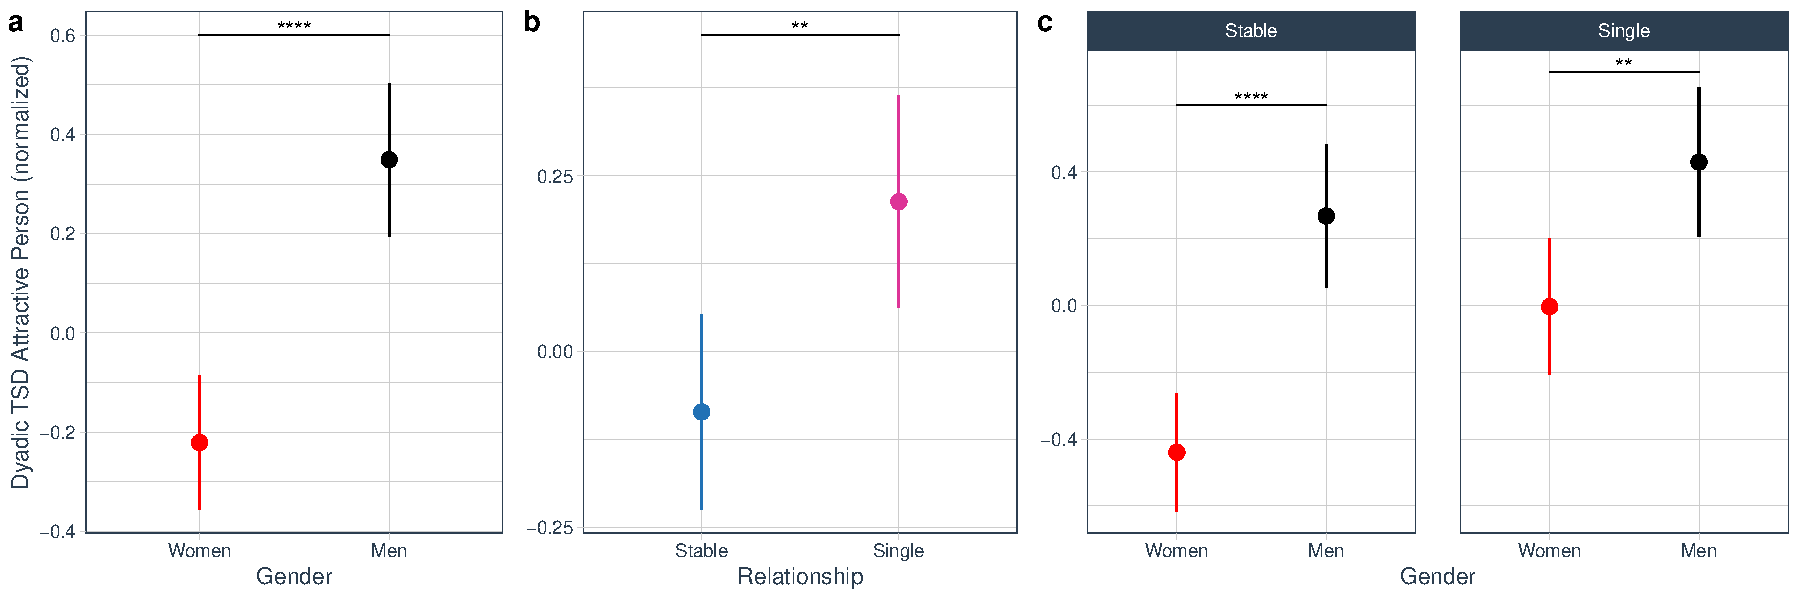
\includegraphics{Sexual_Desire_Arousal_anonymous_files/figure-latex/fig-h1b-1.pdf}
\caption{\label{fig:fig-h1b}Effects of gender and relationship type on Dyadic TSD Attractive Person. Dyadic TSD Attractive Person was transformed using ordered quantile normalization \autocite{petersonOrderedQuantileNormalization2020a}. \textbf{(a)} Simple comparison between sexual desire by gender (for detailed results, see Table \ref{tab:tab-m1b-emm1}); \textbf{(b)} Simple comparison between relationship status levels (for detailed results, see Table \ref{tab:tab-m1b-emm2}); \textbf{(c)} Interaction between relationship type and relationship status (see Table \ref{tab:tab-m1b}; for detailed results, see Table \ref{tab:tab-m1b-emm3}). Dots and bars represent estimated marginal means and 95\% CI. In all cases, significant effects are represented with lines and stars: *\emph{p} \textless{} 0.05, **\emph{p} \textless{} 0.01, ***\emph{p} \textless{} 0.001, ****\emph{p} \textless{} 0.0001.}
\end{figure}

\subsubsection{Hypothesis 1c: Dyadic TSD (Partner)}\label{hypothesis1c}

\paragraph{Model the effects of relationship type and gender on Dyadic TSD: Partner}\label{model-the-effects-of-relationship-type-and-gender-on-dyadic-tsd-partner}

We fitted models with both the original (proportion; \texttt{m1c\_prop}) and transformed (normalized; \texttt{m1c\_norm}) TSD scores, and performed posterior predictive checks (PPCs). As shown elsewhere \autocite[e.g.,][]{gabryVisualizationBayesianWorkflow2019}, if simulated data from one model are more similar to the observed outcome, that model is likely to be preferred.

\begin{Shaded}
\begin{Highlighting}[]
\CommentTok{\# Set contrast options for sum coding (useful for ANOVA{-}like interpretation)}
\FunctionTok{options}\NormalTok{(}\AttributeTok{contrasts =} \FunctionTok{c}\NormalTok{(}\StringTok{"contr.sum"}\NormalTok{, }\StringTok{"contr.poly"}\NormalTok{))}

\CommentTok{\# Fit a linear model using the original proportion{-}based Dyadic TSD (Partner) scores}
\NormalTok{m1c\_prop }\OtherTok{\textless{}{-}} \FunctionTok{lm}\NormalTok{(}
  \StringTok{\textasciigrave{}}\AttributeTok{Dyadic TSD Partner (proportion)}\StringTok{\textasciigrave{}} \SpecialCharTok{\textasciitilde{}}\NormalTok{ Gender }\SpecialCharTok{*}\NormalTok{ Relationship,}
  \AttributeTok{data =}\NormalTok{ dat\_m1}
\NormalTok{)}

\CommentTok{\# Fit a linear model using the normalized Dyadic TSD (Partner) scores}
\NormalTok{m1c\_norm }\OtherTok{\textless{}{-}} \FunctionTok{lm}\NormalTok{(}
  \StringTok{\textasciigrave{}}\AttributeTok{Dyadic TSD Partner (normalized)}\StringTok{\textasciigrave{}} \SpecialCharTok{\textasciitilde{}}\NormalTok{ Gender }\SpecialCharTok{*}\NormalTok{ Relationship,}
  \AttributeTok{data =}\NormalTok{ dat\_m1}
\NormalTok{)}
\end{Highlighting}
\end{Shaded}

\subparagraph{Figure \ref{fig:ppc-m1c}: Posterior predictive checks (PPCs) for Hypothesis 1c.}\label{figure-reffigppc-m1c-posterior-predictive-checks-ppcs-for-hypothesis-1c.}

PPCs were performed using the \texttt{check\_model} function from the \texttt{performance} package \autocite{ludecke2021}, and reported in Fig. \ref{fig:ppc-m1c}. Simulated data from the normalized Solitary TSD model (Fig. \ref{fig:ppc-m1c}b) are more similar to the observed outcome, so this model is preferred.

\begin{Shaded}
\begin{Highlighting}[]
\CommentTok{\# Perform posterior predictive checks (PPC) and arrange them into a single figure}
\NormalTok{ppc\_m1c }\OtherTok{\textless{}{-}} \FunctionTok{ggarrange}\NormalTok{(}
  \CommentTok{\# PPC plot for the original (proportion) Dyadic TSD: Partner model}
  \FunctionTok{plot}\NormalTok{(}
    \FunctionTok{check\_model}\NormalTok{(m1c\_prop, }\AttributeTok{panel =} \ConstantTok{FALSE}\NormalTok{, }\AttributeTok{check =} \StringTok{"pp\_check"}\NormalTok{)}\SpecialCharTok{$}\NormalTok{PP\_CHECK,}
    \AttributeTok{colors =} \FunctionTok{c}\NormalTok{(}\StringTok{"red"}\NormalTok{, }\StringTok{"grey30"}\NormalTok{) }\CommentTok{\# Red for observed data, grey for simulated data}
\NormalTok{  ) }\SpecialCharTok{+}
    \FunctionTok{labs}\NormalTok{(}\AttributeTok{title =} \ConstantTok{NULL}\NormalTok{, }\AttributeTok{subtitle =} \ConstantTok{NULL}\NormalTok{) }\SpecialCharTok{+}
    \FunctionTok{theme\_tq}\NormalTok{() }\SpecialCharTok{+}
    \FunctionTok{facet\_wrap}\NormalTok{(}\SpecialCharTok{\textasciitilde{}}\DecValTok{1}\NormalTok{, }\AttributeTok{labeller =} \FunctionTok{as\_labeller}\NormalTok{(}\FunctionTok{c}\NormalTok{(}
      \StringTok{"1"} \OtherTok{=} \StringTok{"Original (proportion) Dyadic TSD: Partner"}
\NormalTok{    ))),}
  \CommentTok{\# PPC plot for the transformed (normalized) Dyadic TSD: Partner model}
  \FunctionTok{plot}\NormalTok{(}
    \FunctionTok{check\_model}\NormalTok{(m1c\_norm, }\AttributeTok{panel =} \ConstantTok{FALSE}\NormalTok{, }\AttributeTok{check =} \StringTok{"pp\_check"}\NormalTok{)}\SpecialCharTok{$}\NormalTok{PP\_CHECK,}
    \AttributeTok{colors =} \FunctionTok{c}\NormalTok{(}\StringTok{"red"}\NormalTok{, }\StringTok{"grey30"}\NormalTok{)}
\NormalTok{  ) }\SpecialCharTok{+}
    \FunctionTok{labs}\NormalTok{(}\AttributeTok{title =} \ConstantTok{NULL}\NormalTok{, }\AttributeTok{subtitle =} \ConstantTok{NULL}\NormalTok{) }\SpecialCharTok{+}
    \FunctionTok{theme\_tq}\NormalTok{() }\SpecialCharTok{+}
    \FunctionTok{facet\_wrap}\NormalTok{(}\SpecialCharTok{\textasciitilde{}}\DecValTok{1}\NormalTok{, }\AttributeTok{labeller =} \FunctionTok{as\_labeller}\NormalTok{(}\FunctionTok{c}\NormalTok{(}
      \StringTok{"1"} \OtherTok{=} \StringTok{"Transformed (normalized) Dyadic TSD: Partner"}
\NormalTok{    ))),}
  \AttributeTok{labels =} \StringTok{"auto"}\NormalTok{, }\CommentTok{\# Automatically label subplots (a, b)}
  \AttributeTok{common.legend =} \ConstantTok{TRUE}\NormalTok{, }\AttributeTok{legend =} \StringTok{"bottom"} \CommentTok{\# Use a common legend at the bottom}
\NormalTok{)}

\CommentTok{\# Display the final PPC figure}
\NormalTok{ppc\_m1c}
\end{Highlighting}
\end{Shaded}

\begin{figure}
\centering
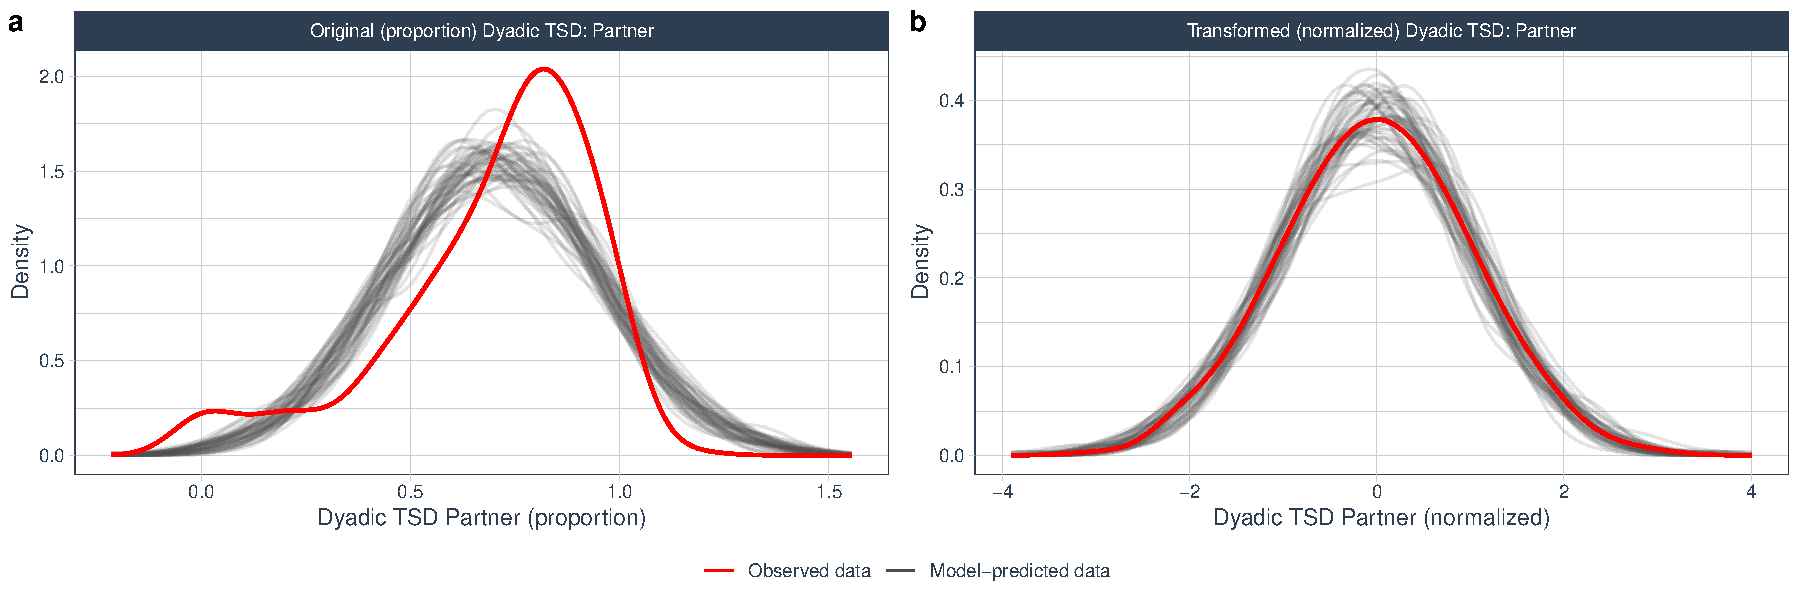
\includegraphics{Sexual_Desire_Arousal_anonymous_files/figure-latex/ppc-m1c-1.pdf}
\caption{\label{fig:ppc-m1c}Posterior predictive check. \textbf{(a)} Original (proportion) Solitary TSD; \textbf{(b)} Transformed (normalized) Solitary TSD. In both panels, red lines represent the observed data, and thin black lines represent 50 iterations of simulated data from each model.}
\end{figure}

\paragraph{\texorpdfstring{Table \ref{tab:tab-m1c}. ANOVA-type table for the interaction between \texttt{Relationship\ type}, and \texttt{Gender}}{Table \ref{tab:tab-m1c}. ANOVA-type table for the interaction between Relationship type, and Gender}}\label{table-reftabtab-m1c.-anova-type-table-for-the-interaction-between-relationship-type-and-gender}

This tables summarizes the results of the model.

\begin{Shaded}
\begin{Highlighting}[]
\CommentTok{\# Generate an ANOVA table summarizing the effects of Relationship Type and Gender on}
\CommentTok{\# Dyadic TSD Partner}
\FunctionTok{anova.sig.lm}\NormalTok{(}
  \AttributeTok{model =}\NormalTok{ m1c\_norm,}
  \AttributeTok{custom\_caption =} \StringTok{"Effects of relationship type and gender on Dyadic TSD Partner"}
\NormalTok{)}
\end{Highlighting}
\end{Shaded}

\begin{table}[H]
\centering
\caption{\label{tab:tab-m1c}Effects of relationship type and gender on Dyadic TSD Partner}
\centering
\resizebox{\ifdim\width>\linewidth\linewidth\else\width\fi}{!}{
\begin{threeparttable}
\begin{tabular}[t]{lcccc}
\toprule
Effect & $df$ & $F$ & $p$ & $\epsilon^2_p$\\
\midrule
Gender & 1, 316 & 15.49 & \textbf{< 0.001} & 0.0365\\
Relationship & 1, 316 & 31.60 & \textbf{< 0.0001} & 0.09\\
Gender × Relationship & 1, 316 & 0.00 & 0.98 & < 0.0001\\
\bottomrule
\end{tabular}
\begin{tablenotes}[para]
\item \textit{Note: } 
\item Sexual desire was transformed using an ordered quantile normalization (\cite{petersonOrderedQuantileNormalization2020a}). Results are Type III ANOVA. $R^2$ = 0.125, $R^2_{adjusted}$ = 0.117. Gender = participant's gender (women, men); Relationship = relationship type (stable, single). As effect size, we report partial epsilon squared ($\epsilon^2_p$), a less biased estimate than $\eta^2$ (see \cite{albersWhenPowerAnalyses2018}). Significant effects are in bold.
\end{tablenotes}
\end{threeparttable}}
\end{table}

\paragraph{\texorpdfstring{\emph{Post-hoc} comparisons}{Post-hoc comparisons}}\label{post-hoc-comparisons-2}

Because the main effects of gender and relationship type, but not their interaction, are significant, we explored these effects using estimated marginal means.

\subparagraph{Table \ref{tab:tab-m1c-emm1}. Estimated marginal means and contrasts between participants' gender.}\label{table-reftabtab-m1c-emm1.-estimated-marginal-means-and-contrasts-between-participants-gender.}

Table of estimated marginal means and contrasts between genders. All estimated marginal means and contrasts were calculated using the \texttt{emmeans} function from the \texttt{emmeans} package \autocite{emmeanscit}.

\begin{Shaded}
\begin{Highlighting}[]
\CommentTok{\# Compute estimated marginal means (EMMs) for Gender from the model}
\NormalTok{emms.m1c1 }\OtherTok{\textless{}{-}} \FunctionTok{emmeans}\NormalTok{(m1c\_norm, }\SpecialCharTok{\textasciitilde{}}\NormalTok{Gender)}

\CommentTok{\# Convert EMM results to a tibble for easier manipulation}
\NormalTok{emms.m1c1.tab }\OtherTok{\textless{}{-}} \FunctionTok{tibble}\NormalTok{(}\FunctionTok{data.frame}\NormalTok{(emms.m1c1))}

\CommentTok{\# Compute post{-}hoc contrasts and format p{-}values}
\NormalTok{t.m1c1 }\OtherTok{\textless{}{-}} \FunctionTok{contr.stars}\NormalTok{(emms.m1c1) }\SpecialCharTok{|\textgreater{}}
  \FunctionTok{mutate}\NormalTok{(}\AttributeTok{p.value =} \FunctionTok{pval.lev}\NormalTok{(p.value)) }\CommentTok{\# Format p{-}values for LaTeX}

\CommentTok{\# Merge EMM and contrast results, clean column names, and format output}
\FunctionTok{merge}\NormalTok{(emms.m1c1.tab, t.m1c1, }\AttributeTok{by =} \DecValTok{0}\NormalTok{, }\AttributeTok{all =} \ConstantTok{TRUE}\NormalTok{) }\SpecialCharTok{|\textgreater{}}
  \FunctionTok{select}\NormalTok{(}\SpecialCharTok{{-}}\FunctionTok{c}\NormalTok{(}\DecValTok{1}\NormalTok{, }\DecValTok{15}\NormalTok{)) }\SpecialCharTok{|\textgreater{}} \CommentTok{\# Remove unnecessary columns}
  \FunctionTok{unite}\NormalTok{(Contrast, group1, group2, }\AttributeTok{sep =} \StringTok{" {-} "}\NormalTok{) }\SpecialCharTok{|\textgreater{}} \CommentTok{\# Create contrast labels}
  \FunctionTok{mutate\_at}\NormalTok{(}\StringTok{"Contrast"}\NormalTok{, str\_replace\_all, }\StringTok{"NA {-} NA"}\NormalTok{, }\StringTok{" "}\NormalTok{) }\SpecialCharTok{|\textgreater{}} \CommentTok{\# Replace missing contrasts}
  \CommentTok{\# Create formatted table}
  \FunctionTok{kable}\NormalTok{(}
    \AttributeTok{digits =} \DecValTok{2}\NormalTok{, }\AttributeTok{booktabs =} \ConstantTok{TRUE}\NormalTok{, }\AttributeTok{align =} \FunctionTok{c}\NormalTok{(}\StringTok{"l"}\NormalTok{, }\FunctionTok{rep}\NormalTok{(}\StringTok{"c"}\NormalTok{, }\DecValTok{5}\NormalTok{), }\StringTok{"l"}\NormalTok{, }\FunctionTok{rep}\NormalTok{(}\StringTok{"c"}\NormalTok{, }\DecValTok{5}\NormalTok{)), }
    \AttributeTok{linesep =} \StringTok{""}\NormalTok{,}
    \AttributeTok{caption =} \StringTok{"Estimated marginal means and contrasts between participants\textquotesingle{} gender"}\NormalTok{,}
    \AttributeTok{escape =} \ConstantTok{FALSE}\NormalTok{,}
    \AttributeTok{col.names =} \FunctionTok{c}\NormalTok{(}
      \StringTok{"Gender"}\NormalTok{, }\StringTok{"EMM"}\NormalTok{, }\StringTok{"$SE$"}\NormalTok{, }\StringTok{"$df$"}\NormalTok{, }\StringTok{"$2.5}\SpecialCharTok{\textbackslash{}\textbackslash{}}\StringTok{\% CI$"}\NormalTok{, }\StringTok{"$97.5}\SpecialCharTok{\textbackslash{}\textbackslash{}}\StringTok{\% CI$"}\NormalTok{,}
      \StringTok{"Contrast"}\NormalTok{, }\StringTok{"Difference"}\NormalTok{, }\StringTok{"$SE$"}\NormalTok{, }\StringTok{"$df$"}\NormalTok{, }\StringTok{"$t$"}\NormalTok{, }\StringTok{"$p$"}
\NormalTok{    )}
\NormalTok{  ) }\SpecialCharTok{|\textgreater{}}
  \CommentTok{\# Add a header separating EMMs and contrasts}
  \FunctionTok{add\_header\_above}\NormalTok{(}\FunctionTok{c}\NormalTok{(}\StringTok{" "} \OtherTok{=} \DecValTok{6}\NormalTok{, }\StringTok{"Contrasts"} \OtherTok{=} \DecValTok{6}\NormalTok{)) }\SpecialCharTok{|\textgreater{}}
  \CommentTok{\# Apply LaTeX styling for table positioning}
  \FunctionTok{kable\_styling}\NormalTok{(}\AttributeTok{latex\_options =} \FunctionTok{c}\NormalTok{(}\StringTok{"HOLD\_position"}\NormalTok{, }\StringTok{"scale\_down"}\NormalTok{)) }\SpecialCharTok{|\textgreater{}}
  \CommentTok{\# Add footnote explaining significance formatting}
  \FunctionTok{footnote}\NormalTok{(}
    \AttributeTok{general =} \StringTok{"Significant effects are in bold."}\NormalTok{, }\AttributeTok{threeparttable =} \ConstantTok{TRUE}\NormalTok{,}
    \AttributeTok{footnote\_as\_chunk =} \ConstantTok{TRUE}\NormalTok{, }\AttributeTok{escape =} \ConstantTok{FALSE}
\NormalTok{  )}
\end{Highlighting}
\end{Shaded}

\begin{table}[H]
\centering
\caption{\label{tab:tab-m1c-emm1}Estimated marginal means and contrasts between participants' gender}
\centering
\resizebox{\ifdim\width>\linewidth\linewidth\else\width\fi}{!}{
\begin{threeparttable}
\begin{tabular}[t]{lccccclccccc}
\toprule
\multicolumn{6}{c}{ } & \multicolumn{6}{c}{Contrasts} \\
\cmidrule(l{3pt}r{3pt}){7-12}
Gender & EMM & $SE$ & $df$ & $2.5\% CI$ & $97.5\% CI$ & Contrast & Difference & $SE$ & $df$ & $t$ & $p$\\
\midrule
Women & -0.21 & 0.07 & 316 & -0.35 & -0.07 & Women - Men & -0.42 & 0.11 & 316 & -3.94 & \textbf{< 0.001}\\
Men & 0.20 & 0.08 & 316 & 0.05 & 0.36 &  &  &  &  &  & \\
\bottomrule
\end{tabular}
\begin{tablenotes}[para]
\item \textit{Note: } 
\item Significant effects are in bold.
\end{tablenotes}
\end{threeparttable}}
\end{table}

\subparagraph{Table \ref{tab:tab-m1c-emm2}. Estimated marginal means and contrasts between relationship status.}\label{table-reftabtab-m1c-emm2.-estimated-marginal-means-and-contrasts-between-relationship-status.}

Table of estimated marginal means and contrasts between relationship status. All estimated marginal means and contrasts were calculated using the \texttt{emmeans} function from the \texttt{emmeans} package \autocite{emmeanscit}.

\begin{Shaded}
\begin{Highlighting}[]
\CommentTok{\# Compute estimated marginal means (EMMs) for Relationship Status from the model}
\NormalTok{emms.m1c2 }\OtherTok{\textless{}{-}} \FunctionTok{emmeans}\NormalTok{(m1c\_norm, }\SpecialCharTok{\textasciitilde{}}\NormalTok{Relationship)}

\CommentTok{\# Convert EMM results to a tibble for easier manipulation}
\NormalTok{emms.m1c2.tab }\OtherTok{\textless{}{-}} \FunctionTok{tibble}\NormalTok{(}\FunctionTok{data.frame}\NormalTok{(emms.m1c2))}

\CommentTok{\# Compute post{-}hoc contrasts and format p{-}values}
\NormalTok{t.m1c2 }\OtherTok{\textless{}{-}} \FunctionTok{contr.stars}\NormalTok{(emms.m1c2) }\SpecialCharTok{|\textgreater{}}
  \FunctionTok{mutate}\NormalTok{(}\AttributeTok{p.value =} \FunctionTok{pval.lev}\NormalTok{(p.value)) }\CommentTok{\# Format p{-}values for LaTeX}

\CommentTok{\# Merge EMM and contrast results, clean column names, and format output}
\FunctionTok{merge}\NormalTok{(emms.m1c2.tab, t.m1c2, }\AttributeTok{by =} \DecValTok{0}\NormalTok{, }\AttributeTok{all =} \ConstantTok{TRUE}\NormalTok{) }\SpecialCharTok{|\textgreater{}}
  \FunctionTok{select}\NormalTok{(}\SpecialCharTok{{-}}\FunctionTok{c}\NormalTok{(}\DecValTok{1}\NormalTok{, }\DecValTok{15}\NormalTok{)) }\SpecialCharTok{|\textgreater{}} \CommentTok{\# Remove unnecessary columns}
  \FunctionTok{unite}\NormalTok{(Contrast, group1, group2, }\AttributeTok{sep =} \StringTok{" {-} "}\NormalTok{) }\SpecialCharTok{|\textgreater{}} \CommentTok{\# Create contrast labels}
  \FunctionTok{mutate\_at}\NormalTok{(}\StringTok{"Contrast"}\NormalTok{, str\_replace\_all, }\StringTok{"NA {-} NA"}\NormalTok{, }\StringTok{" "}\NormalTok{) }\SpecialCharTok{|\textgreater{}} \CommentTok{\# Replace missing contrasts}
  \CommentTok{\# Create formatted table}
  \FunctionTok{kable}\NormalTok{(}
    \AttributeTok{digits =} \DecValTok{2}\NormalTok{, }\AttributeTok{booktabs =} \ConstantTok{TRUE}\NormalTok{, }\AttributeTok{align =} \FunctionTok{c}\NormalTok{(}\StringTok{"l"}\NormalTok{, }\FunctionTok{rep}\NormalTok{(}\StringTok{"c"}\NormalTok{, }\DecValTok{5}\NormalTok{), }\StringTok{"l"}\NormalTok{, }\FunctionTok{rep}\NormalTok{(}\StringTok{"c"}\NormalTok{, }\DecValTok{5}\NormalTok{)), }
    \AttributeTok{linesep =} \StringTok{""}\NormalTok{,}
    \AttributeTok{caption =} \StringTok{"Estimated marginal means and contrasts between relationship status"}\NormalTok{,}
    \AttributeTok{escape =} \ConstantTok{FALSE}\NormalTok{,}
    \AttributeTok{col.names =} \FunctionTok{c}\NormalTok{(}
      \StringTok{"Relationship type"}\NormalTok{, }\StringTok{"EMM"}\NormalTok{, }\StringTok{"$SE$"}\NormalTok{, }\StringTok{"$df$"}\NormalTok{, }\StringTok{"$2.5}\SpecialCharTok{\textbackslash{}\textbackslash{}}\StringTok{\% CI$"}\NormalTok{, }\StringTok{"$97.5}\SpecialCharTok{\textbackslash{}\textbackslash{}}\StringTok{\% CI$"}\NormalTok{,}
      \StringTok{"Contrast"}\NormalTok{, }\StringTok{"Difference"}\NormalTok{, }\StringTok{"$SE$"}\NormalTok{, }\StringTok{"$df$"}\NormalTok{, }\StringTok{"$t$"}\NormalTok{, }\StringTok{"$p$"}
\NormalTok{    )}
\NormalTok{  ) }\SpecialCharTok{|\textgreater{}}
  \CommentTok{\# Add a header separating EMMs and contrasts}
  \FunctionTok{add\_header\_above}\NormalTok{(}\FunctionTok{c}\NormalTok{(}\StringTok{" "} \OtherTok{=} \DecValTok{6}\NormalTok{, }\StringTok{"Contrasts"} \OtherTok{=} \DecValTok{6}\NormalTok{)) }\SpecialCharTok{|\textgreater{}}
  \CommentTok{\# Apply LaTeX styling for table positioning}
  \FunctionTok{kable\_styling}\NormalTok{(}\AttributeTok{latex\_options =} \FunctionTok{c}\NormalTok{(}\StringTok{"HOLD\_position"}\NormalTok{, }\StringTok{"scale\_down"}\NormalTok{)) }\SpecialCharTok{|\textgreater{}}
  \CommentTok{\# Add footnote explaining significance formatting}
  \FunctionTok{footnote}\NormalTok{(}
    \AttributeTok{general =} \StringTok{"Significant effects are in bold."}\NormalTok{, }\AttributeTok{threeparttable =} \ConstantTok{TRUE}\NormalTok{,}
    \AttributeTok{footnote\_as\_chunk =} \ConstantTok{TRUE}\NormalTok{, }\AttributeTok{escape =} \ConstantTok{FALSE}
\NormalTok{  )}
\end{Highlighting}
\end{Shaded}

\begin{table}[H]
\centering
\caption{\label{tab:tab-m1c-emm2}Estimated marginal means and contrasts between relationship status}
\centering
\resizebox{\ifdim\width>\linewidth\linewidth\else\width\fi}{!}{
\begin{threeparttable}
\begin{tabular}[t]{lccccclccccc}
\toprule
\multicolumn{6}{c}{ } & \multicolumn{6}{c}{Contrasts} \\
\cmidrule(l{3pt}r{3pt}){7-12}
Relationship type & EMM & $SE$ & $df$ & $2.5\% CI$ & $97.5\% CI$ & Contrast & Difference & $SE$ & $df$ & $t$ & $p$\\
\midrule
Stable & 0.29 & 0.07 & 316 & 0.15 & 0.43 & Stable - Single & 0.6 & 0.11 & 316 & 5.62 & \textbf{< 0.0001}\\
Single & -0.30 & 0.08 & 316 & -0.46 & -0.15 &  &  &  &  &  & \\
\bottomrule
\end{tabular}
\begin{tablenotes}[para]
\item \textit{Note: } 
\item Significant effects are in bold.
\end{tablenotes}
\end{threeparttable}}
\end{table}

\subparagraph{Table \ref{tab:tab-m1c-emm3}. Estimated marginal means and contrasts between gender by relationship status.}\label{table-reftabtab-m1c-emm3.-estimated-marginal-means-and-contrasts-between-gender-by-relationship-status.}

Table of estimated marginal means and contrasts between gender by relationship status. All estimated marginal means and contrasts were calculated using the \texttt{emmeans} function from the \texttt{emmeans} package \autocite{emmeanscit}.

\begin{Shaded}
\begin{Highlighting}[]
\CommentTok{\# Compute estimated marginal means (EMMs) for Gender within each Relationship Status}
\NormalTok{emms.m1c3 }\OtherTok{\textless{}{-}} \FunctionTok{emmeans}\NormalTok{(m1c\_norm, }\SpecialCharTok{\textasciitilde{}}\NormalTok{ Gender }\SpecialCharTok{|}\NormalTok{ Relationship)}

\CommentTok{\# Convert EMM results to a tibble for easier manipulation}
\NormalTok{emms.m1c3.tab }\OtherTok{\textless{}{-}} \FunctionTok{tibble}\NormalTok{(}\FunctionTok{data.frame}\NormalTok{(emms.m1c3))}

\CommentTok{\# Compute post{-}hoc contrasts and format p{-}values}
\NormalTok{t.m1c3 }\OtherTok{\textless{}{-}} \FunctionTok{contr.stars}\NormalTok{(emms.m1c3) }\SpecialCharTok{|\textgreater{}}
  \FunctionTok{mutate}\NormalTok{(}\AttributeTok{p.value =} \FunctionTok{pval.lev}\NormalTok{(p.value)) }\CommentTok{\# Format p{-}values for LaTeX}

\CommentTok{\# Insert NA rows to maintain table structure for grouped relationship status display}
\NormalTok{t.m1c3.f }\OtherTok{\textless{}{-}}\NormalTok{ t.m1c3 }\SpecialCharTok{|\textgreater{}}
  \FunctionTok{insertRows}\NormalTok{(}\DecValTok{2}\NormalTok{, }\AttributeTok{new =} \ConstantTok{NA}\NormalTok{) }\SpecialCharTok{|\textgreater{}} \CommentTok{\# Insert empty row after first contrast}
  \FunctionTok{insertRows}\NormalTok{(}\DecValTok{4}\NormalTok{, }\AttributeTok{new =} \ConstantTok{NA}\NormalTok{) }\CommentTok{\# Insert empty row after second contrast}

\CommentTok{\# Merge EMM and contrast results, clean column names, and format output}
\FunctionTok{merge}\NormalTok{(emms.m1c3.tab, t.m1c3.f, }\AttributeTok{by =} \DecValTok{0}\NormalTok{, }\AttributeTok{all =} \ConstantTok{TRUE}\NormalTok{) }\SpecialCharTok{|\textgreater{}}
  \FunctionTok{select}\NormalTok{(}\SpecialCharTok{{-}}\FunctionTok{c}\NormalTok{(}\DecValTok{1}\NormalTok{, }\DecValTok{3}\NormalTok{, }\DecValTok{11}\NormalTok{, }\DecValTok{17}\NormalTok{)) }\SpecialCharTok{|\textgreater{}} \CommentTok{\# Remove unnecessary columns}
  \FunctionTok{drop\_na}\NormalTok{(Gender) }\SpecialCharTok{|\textgreater{}} \CommentTok{\# Ensure Gender column is complete}
  \FunctionTok{unite}\NormalTok{(Contrast, group1, group2, }\AttributeTok{sep =} \StringTok{" {-} "}\NormalTok{) }\SpecialCharTok{|\textgreater{}} \CommentTok{\# Create contrast labels}
  \FunctionTok{mutate\_at}\NormalTok{(}\StringTok{"Contrast"}\NormalTok{, str\_replace\_all, }\StringTok{"NA {-} NA"}\NormalTok{, }\StringTok{""}\NormalTok{) }\SpecialCharTok{|\textgreater{}} \CommentTok{\# Replace missing contrasts}
  \CommentTok{\# Create formatted table}
  \FunctionTok{kable}\NormalTok{(}
    \AttributeTok{digits =} \DecValTok{2}\NormalTok{, }\AttributeTok{booktabs =} \ConstantTok{TRUE}\NormalTok{, }\AttributeTok{align =} \FunctionTok{c}\NormalTok{(}\StringTok{"l"}\NormalTok{, }\StringTok{"l"}\NormalTok{, }\FunctionTok{rep}\NormalTok{(}\StringTok{"c"}\NormalTok{, }\DecValTok{5}\NormalTok{), }\StringTok{"l"}\NormalTok{, }\FunctionTok{rep}\NormalTok{(}\StringTok{"c"}\NormalTok{, }\DecValTok{5}\NormalTok{)), }
    \AttributeTok{linesep =} \StringTok{""}\NormalTok{,}
    \AttributeTok{caption =} \StringTok{"Estimated marginal means and contrasts between gender by relationship status"}\NormalTok{,}
    \AttributeTok{escape =} \ConstantTok{FALSE}\NormalTok{,}
    \AttributeTok{col.names =} \FunctionTok{c}\NormalTok{(}
      \StringTok{"Gender"}\NormalTok{, }\StringTok{"EMM"}\NormalTok{, }\StringTok{"$SE$"}\NormalTok{, }\StringTok{"$df$"}\NormalTok{, }\StringTok{"$2.5}\SpecialCharTok{\textbackslash{}\textbackslash{}}\StringTok{\% CI$"}\NormalTok{, }\StringTok{"$97.5}\SpecialCharTok{\textbackslash{}\textbackslash{}}\StringTok{\% CI$"}\NormalTok{,}
      \StringTok{"Contrast"}\NormalTok{, }\StringTok{"Difference"}\NormalTok{, }\StringTok{"$SE$"}\NormalTok{, }\StringTok{"$df$"}\NormalTok{, }\StringTok{"$t$"}\NormalTok{, }\StringTok{"$p$"}
\NormalTok{    )}
\NormalTok{  ) }\SpecialCharTok{|\textgreater{}}
  \CommentTok{\# Add grouped row labels for Relationship Status}
  \FunctionTok{pack\_rows}\NormalTok{(}\StringTok{"Relationship status: Stable"}\NormalTok{,}
    \AttributeTok{start\_row =} \DecValTok{1}\NormalTok{, }\AttributeTok{end\_row =} \DecValTok{2}\NormalTok{,}
    \AttributeTok{bold =} \ConstantTok{FALSE}\NormalTok{, }\AttributeTok{background =} \StringTok{"lightgray"}
\NormalTok{  ) }\SpecialCharTok{|\textgreater{}}
  \FunctionTok{pack\_rows}\NormalTok{(}\StringTok{"Relationship status: Single"}\NormalTok{,}
    \AttributeTok{start\_row =} \DecValTok{3}\NormalTok{, }\AttributeTok{end\_row =} \DecValTok{4}\NormalTok{,}
    \AttributeTok{bold =} \ConstantTok{FALSE}\NormalTok{, }\AttributeTok{background =} \StringTok{"lightgray"}
\NormalTok{  ) }\SpecialCharTok{|\textgreater{}}
  \CommentTok{\# Add a header separating EMMs and contrasts}
  \FunctionTok{add\_header\_above}\NormalTok{(}\FunctionTok{c}\NormalTok{(}\StringTok{" "} \OtherTok{=} \DecValTok{6}\NormalTok{, }\StringTok{"Contrasts"} \OtherTok{=} \DecValTok{6}\NormalTok{)) }\SpecialCharTok{|\textgreater{}}
  \CommentTok{\# Apply LaTeX styling for table positioning}
  \FunctionTok{kable\_styling}\NormalTok{(}\AttributeTok{latex\_options =} \FunctionTok{c}\NormalTok{(}\StringTok{"HOLD\_position"}\NormalTok{, }\StringTok{"scale\_down"}\NormalTok{)) }\SpecialCharTok{|\textgreater{}}
  \CommentTok{\# Add footnote explaining significance formatting}
  \FunctionTok{footnote}\NormalTok{(}
    \AttributeTok{general =} \StringTok{"Significant effects are in bold."}\NormalTok{, }\AttributeTok{threeparttable =} \ConstantTok{TRUE}\NormalTok{,}
    \AttributeTok{footnote\_as\_chunk =} \ConstantTok{TRUE}\NormalTok{, }\AttributeTok{escape =} \ConstantTok{FALSE}
\NormalTok{  )}
\end{Highlighting}
\end{Shaded}

\begin{table}[H]
\centering
\caption{\label{tab:tab-m1c-emm3}Estimated marginal means and contrasts between gender by relationship status}
\centering
\resizebox{\ifdim\width>\linewidth\linewidth\else\width\fi}{!}{
\begin{threeparttable}
\begin{tabular}[t]{llccccclcccc}
\toprule
\multicolumn{6}{c}{ } & \multicolumn{6}{c}{Contrasts} \\
\cmidrule(l{3pt}r{3pt}){7-12}
Gender & EMM & $SE$ & $df$ & $2.5\% CI$ & $97.5\% CI$ & Contrast & Difference & $SE$ & $df$ & $t$ & $p$\\
\midrule
\addlinespace[0.3em]
\multicolumn{12}{l}{\cellcolor{lightgray}{Relationship status: Stable}}\\
\hspace{1em}Women & 0.09 & 0.09 & 316 & -0.09 & 0.27 & Women - Men & -0.41 & 0.14 & 316 & -2.90 & \textbf{0.004}\\
\hspace{1em}Men & 0.50 & 0.11 & 316 & 0.28 & 0.72 &  &  &  &  &  & \\
\addlinespace[0.3em]
\multicolumn{12}{l}{\cellcolor{lightgray}{Relationship status: Single}}\\
\hspace{1em}Women & -0.51 & 0.11 & 316 & -0.72 & -0.30 & Women - Men & -0.42 & 0.16 & 316 & -2.68 & \textbf{0.0077}\\
\hspace{1em}Men & -0.09 & 0.11 & 316 & -0.32 & 0.13 &  &  &  &  &  & \\
\bottomrule
\end{tabular}
\begin{tablenotes}[para]
\item \textit{Note: } 
\item Significant effects are in bold.
\end{tablenotes}
\end{threeparttable}}
\end{table}

\paragraph{Figure \ref{fig:fig-h1c}. Effects of gender and relationship type on Dyadic TSD Partner}\label{figure-reffigfig-h1c.-effects-of-gender-and-relationship-type-on-dyadic-tsd-partner}

This figure summarizes the results of hypothesis 1c.

\begin{Shaded}
\begin{Highlighting}[]
\CommentTok{\# Plot (a): Main effect of Gender on Dyadic TSD Partner}
\NormalTok{h1c1 }\OtherTok{\textless{}{-}} \FunctionTok{ggplot}\NormalTok{(dat\_m1, }\FunctionTok{aes}\NormalTok{(}
  \AttributeTok{x =}\NormalTok{ Gender, }\AttributeTok{y =} \StringTok{\textasciigrave{}}\AttributeTok{Dyadic TSD Partner (normalized)}\StringTok{\textasciigrave{}}\NormalTok{, }\AttributeTok{color =}\NormalTok{ Gender}
\NormalTok{)) }\SpecialCharTok{+}
  \FunctionTok{scale\_color\_manual}\NormalTok{(}\AttributeTok{values =}\NormalTok{ color.Gender) }\SpecialCharTok{+}
  \FunctionTok{scale\_fill\_manual}\NormalTok{(}\AttributeTok{values =}\NormalTok{ color.Gender) }\SpecialCharTok{+}
  \FunctionTok{geom\_linerange}\NormalTok{(}
    \AttributeTok{data =}\NormalTok{ emms.m1c1.tab }\SpecialCharTok{|\textgreater{}} \FunctionTok{rename}\NormalTok{(}\StringTok{"Dyadic TSD Partner (normalized)"} \OtherTok{=}\NormalTok{ emmean),}
    \AttributeTok{mapping =} \FunctionTok{aes}\NormalTok{(}\AttributeTok{ymin =}\NormalTok{ lower.CL, }\AttributeTok{ymax =}\NormalTok{ upper.CL)}
\NormalTok{  ) }\SpecialCharTok{+}
  \FunctionTok{geom\_point}\NormalTok{(}
    \AttributeTok{data =}\NormalTok{ emms.m1c1.tab }\SpecialCharTok{|\textgreater{}} \FunctionTok{rename}\NormalTok{(}\StringTok{"Dyadic TSD Partner (normalized)"} \OtherTok{=}\NormalTok{ emmean),}
    \AttributeTok{position =} \FunctionTok{position\_dodge}\NormalTok{(}\FloatTok{0.1}\NormalTok{), }\AttributeTok{size =} \DecValTok{3}
\NormalTok{  ) }\SpecialCharTok{+}
  \FunctionTok{stat\_pvalue\_manual}\NormalTok{(t.m1c1, }\AttributeTok{label =} \StringTok{"p.signif"}\NormalTok{, }\AttributeTok{y.position =} \FloatTok{0.4}\NormalTok{, }\AttributeTok{tip.length =} \DecValTok{0}\NormalTok{) }\SpecialCharTok{+}
  \FunctionTok{guides}\NormalTok{(}\AttributeTok{color =} \StringTok{"none"}\NormalTok{) }\SpecialCharTok{+}
  \FunctionTok{theme\_tq}\NormalTok{()}

\CommentTok{\# Plot (b): Main effect of Relationship on Dyadic TSD Partner}
\NormalTok{h1c2 }\OtherTok{\textless{}{-}} \FunctionTok{ggplot}\NormalTok{(dat\_m1, }\FunctionTok{aes}\NormalTok{(}
  \AttributeTok{x =}\NormalTok{ Relationship, }\AttributeTok{y =} \StringTok{\textasciigrave{}}\AttributeTok{Dyadic TSD Partner (normalized)}\StringTok{\textasciigrave{}}\NormalTok{, }\AttributeTok{color =}\NormalTok{ Relationship}
\NormalTok{)) }\SpecialCharTok{+}
  \FunctionTok{scale\_color\_manual}\NormalTok{(}\AttributeTok{values =}\NormalTok{ color.Relationship) }\SpecialCharTok{+}
  \FunctionTok{scale\_fill\_manual}\NormalTok{(}\AttributeTok{values =}\NormalTok{ color.Relationship) }\SpecialCharTok{+}
  \FunctionTok{geom\_linerange}\NormalTok{(}
    \AttributeTok{data =}\NormalTok{ emms.m1c2.tab }\SpecialCharTok{|\textgreater{}} \FunctionTok{rename}\NormalTok{(}\StringTok{"Dyadic TSD Partner (normalized)"} \OtherTok{=}\NormalTok{ emmean),}
    \AttributeTok{mapping =} \FunctionTok{aes}\NormalTok{(}\AttributeTok{ymin =}\NormalTok{ lower.CL, }\AttributeTok{ymax =}\NormalTok{ upper.CL)}
\NormalTok{  ) }\SpecialCharTok{+}
  \FunctionTok{geom\_point}\NormalTok{(}
    \AttributeTok{data =}\NormalTok{ emms.m1c2.tab }\SpecialCharTok{|\textgreater{}} \FunctionTok{rename}\NormalTok{(}\StringTok{"Dyadic TSD Partner (normalized)"} \OtherTok{=}\NormalTok{ emmean),}
    \AttributeTok{position =} \FunctionTok{position\_dodge}\NormalTok{(}\FloatTok{0.1}\NormalTok{), }\AttributeTok{size =} \DecValTok{3}
\NormalTok{  ) }\SpecialCharTok{+}
  \FunctionTok{stat\_pvalue\_manual}\NormalTok{(t.m1c2, }\AttributeTok{label =} \StringTok{"p.signif"}\NormalTok{, }\AttributeTok{y.position =} \FloatTok{0.5}\NormalTok{, }\AttributeTok{tip.length =} \DecValTok{0}\NormalTok{) }\SpecialCharTok{+}
  \FunctionTok{guides}\NormalTok{(}\AttributeTok{color =} \StringTok{"none"}\NormalTok{) }\SpecialCharTok{+}
  \FunctionTok{theme\_tq}\NormalTok{()}

\CommentTok{\# Plot (c): Gender × Relationship Interaction on Dyadic TSD Partner}
\NormalTok{h1c3 }\OtherTok{\textless{}{-}} \FunctionTok{ggplot}\NormalTok{(dat\_m1, }\FunctionTok{aes}\NormalTok{(}
  \AttributeTok{x =}\NormalTok{ Gender, }\AttributeTok{y =} \StringTok{\textasciigrave{}}\AttributeTok{Dyadic TSD Partner (normalized)}\StringTok{\textasciigrave{}}\NormalTok{, }\AttributeTok{color =}\NormalTok{ Gender}
\NormalTok{)) }\SpecialCharTok{+}
  \FunctionTok{scale\_color\_manual}\NormalTok{(}\AttributeTok{values =}\NormalTok{ color.Gender) }\SpecialCharTok{+}
  \FunctionTok{scale\_fill\_manual}\NormalTok{(}\AttributeTok{values =}\NormalTok{ color.Gender) }\SpecialCharTok{+}
  \FunctionTok{facet\_wrap}\NormalTok{(}\SpecialCharTok{\textasciitilde{}}\NormalTok{Relationship) }\SpecialCharTok{+}
  \FunctionTok{geom\_linerange}\NormalTok{(}
    \AttributeTok{data =}\NormalTok{ emms.m1c3.tab }\SpecialCharTok{|\textgreater{}} \FunctionTok{rename}\NormalTok{(}\StringTok{"Dyadic TSD Partner (normalized)"} \OtherTok{=}\NormalTok{ emmean),}
    \AttributeTok{mapping =} \FunctionTok{aes}\NormalTok{(}\AttributeTok{ymin =}\NormalTok{ lower.CL, }\AttributeTok{ymax =}\NormalTok{ upper.CL)}
\NormalTok{  ) }\SpecialCharTok{+}
  \FunctionTok{geom\_point}\NormalTok{(}
    \AttributeTok{data =}\NormalTok{ emms.m1c3.tab }\SpecialCharTok{|\textgreater{}} \FunctionTok{rename}\NormalTok{(}\StringTok{"Dyadic TSD Partner (normalized)"} \OtherTok{=}\NormalTok{ emmean),}
    \AttributeTok{position =} \FunctionTok{position\_dodge}\NormalTok{(}\FloatTok{0.1}\NormalTok{), }\AttributeTok{size =} \DecValTok{3}
\NormalTok{  ) }\SpecialCharTok{+}
  \FunctionTok{stat\_pvalue\_manual}\NormalTok{(t.m1c3, }\AttributeTok{label =} \StringTok{"p.signif"}\NormalTok{, }\AttributeTok{y.position =} \FunctionTok{c}\NormalTok{(}\FloatTok{0.8}\NormalTok{, }\FloatTok{0.2}\NormalTok{), }\AttributeTok{tip.length =} \DecValTok{0}\NormalTok{) }\SpecialCharTok{+}
  \FunctionTok{guides}\NormalTok{(}\AttributeTok{color =} \StringTok{"none"}\NormalTok{) }\SpecialCharTok{+}
  \FunctionTok{theme\_tq}\NormalTok{()}

\CommentTok{\# Combine the three plots into a single figure}
\NormalTok{p1c }\OtherTok{\textless{}{-}} \FunctionTok{ggarrange}\NormalTok{(h1c1, h1c2 }\SpecialCharTok{+} \FunctionTok{labs}\NormalTok{(}\AttributeTok{y =} \ConstantTok{NULL}\NormalTok{), h1c3 }\SpecialCharTok{+} \FunctionTok{labs}\NormalTok{(}\AttributeTok{y =} \ConstantTok{NULL}\NormalTok{),}
  \AttributeTok{ncol =} \DecValTok{3}\NormalTok{, }\AttributeTok{labels =} \StringTok{"auto"}\NormalTok{, }\AttributeTok{widths =} \FunctionTok{c}\NormalTok{(}\DecValTok{1}\NormalTok{, }\DecValTok{1}\NormalTok{, }\FloatTok{1.5}\NormalTok{) }\CommentTok{\# Adjust widths for better alignment}
\NormalTok{)}

\CommentTok{\# Display the final figure}
\NormalTok{p1c}
\end{Highlighting}
\end{Shaded}

\begin{figure}
\centering
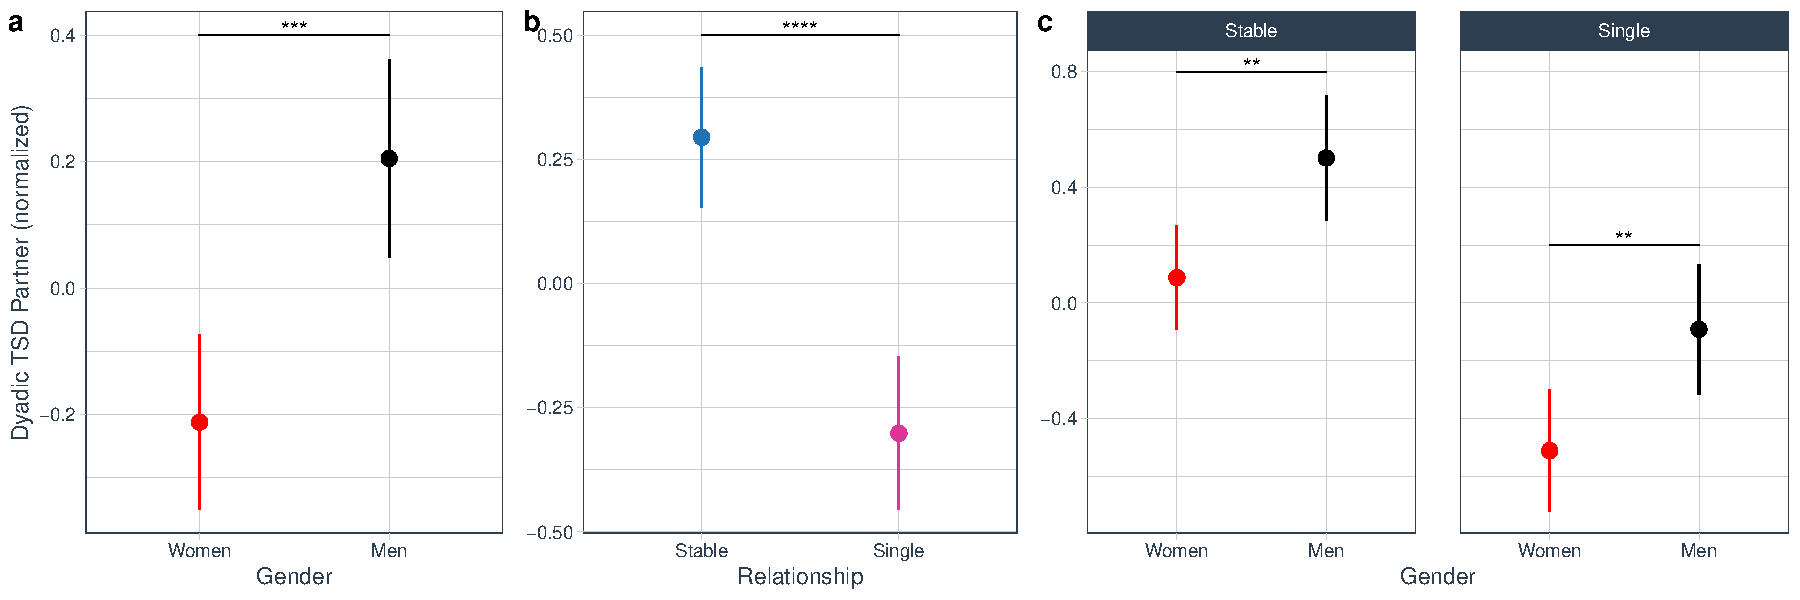
\includegraphics{Sexual_Desire_Arousal_anonymous_files/figure-latex/fig-h1c-1.pdf}
\caption{\label{fig:fig-h1c}Effects of gender and relationship type on Dyadic TSD Partner. Dyadic TSD Partner was transformed using ordered quantile normalization \autocite{petersonOrderedQuantileNormalization2020a}. \textbf{(a)} Simple comparison between sexual desire by gender (for detailed results, see Table \ref{tab:tab-m1c-emm1}); \textbf{(b)} Simple comparison between relationship status levels (for detailed results, see Table \ref{tab:tab-m1c-emm2}); \textbf{(c)} Interaction between relationship type and relationship status (see Table \ref{tab:tab-m1c}; for detailed results, see Table \ref{tab:tab-m1c-emm3}). Dots and bars represent estimated marginal means and 95\% CI. In all cases, significant effects are represented with lines and stars: *\emph{p} \textless{} 0.05, **\emph{p} \textless{} 0.01, ***\emph{p} \textless{} 0.001, ****\emph{p} \textless{} 0.0001.}
\end{figure}

\subsection{Data filtering for hypotheses 2 and 3.}\label{datfil2and3}

To avoid over-complicating the models, first we tested whether the effects of stimuli on sexual arousal were stronger depending on the content of the stimuli (erotic versus non-erotic). This was, in fact, the case.

\subsubsection{Table \ref{tab:tab-m-stimuli-content}. ANOVA-type table for the effects of stimuli content, gender and stimuli sex on Subjective sexual arousal}\label{table-reftabtab-m-stimuli-content.-anova-type-table-for-the-effects-of-stimuli-content-gender-and-stimuli-sex-on-subjective-sexual-arousal}

We fitted a linear mixed model with Gender, Stimuli sex, Stimuli content, and their interactions, as fixed effects for Subjective sexual arousal and including, as random effects, random intercepts per stimulus, as well as random intercepts and slopes for the effect of stimuli content.

\begin{Shaded}
\begin{Highlighting}[]
\CommentTok{\# Fit a linear mixed model predicting Subjective Sexual Arousal}
\CommentTok{\# Fixed effects: Gender, Stimuli sex, Stimuli content, and their interactions}
\CommentTok{\# Random effects: Intercepts per stimulus; intercepts \& slopes for stimuli content per participant}
\NormalTok{m\_stim\_cont }\OtherTok{\textless{}{-}} \FunctionTok{lmer}\NormalTok{(}
  \StringTok{\textasciigrave{}}\AttributeTok{Subjective sexual arousal}\StringTok{\textasciigrave{}} \SpecialCharTok{\textasciitilde{}}\NormalTok{ Gender }\SpecialCharTok{*} \StringTok{\textasciigrave{}}\AttributeTok{Stimuli sex}\StringTok{\textasciigrave{}} \SpecialCharTok{*} \StringTok{\textasciigrave{}}\AttributeTok{Stimuli content}\StringTok{\textasciigrave{}} \SpecialCharTok{+}
\NormalTok{    (}\DecValTok{1} \SpecialCharTok{|} \StringTok{\textasciigrave{}}\AttributeTok{Stimuli code}\StringTok{\textasciigrave{}}\NormalTok{) }\SpecialCharTok{+}
\NormalTok{    (}\DecValTok{1} \SpecialCharTok{+} \StringTok{\textasciigrave{}}\AttributeTok{Stimuli content}\StringTok{\textasciigrave{}} \SpecialCharTok{*} \StringTok{\textasciigrave{}}\AttributeTok{Stimuli sex}\StringTok{\textasciigrave{}} \SpecialCharTok{|}\NormalTok{ Participant),}
  \AttributeTok{data =}\NormalTok{ dat,}
  \AttributeTok{control =} \FunctionTok{lmerControl}\NormalTok{(}\AttributeTok{optimizer =} \StringTok{"bobyqa"}\NormalTok{) }\CommentTok{\# Use "bobyqa" optimizer for better convergence}
\NormalTok{)}

\CommentTok{\# Generate ANOVA table summarizing the model results}
\FunctionTok{anova.sig.lmer}\NormalTok{(}
  \AttributeTok{model =}\NormalTok{ m\_stim\_cont,}
  \AttributeTok{custom\_caption =} \StringTok{"Effects of relationship type, gender and stimuli sex on Dyadic TSD Partner"}
\NormalTok{)}
\end{Highlighting}
\end{Shaded}

\begin{table}[H]
\centering
\caption{\label{tab:tab-m-stimuli-content}Effects of relationship type, gender and stimuli sex on Dyadic TSD Partner}
\centering
\resizebox{\ifdim\width>\linewidth\linewidth\else\width\fi}{!}{
\begin{threeparttable}
\begin{tabular}[t]{lcccc}
\toprule
Effect & $df$ & $F$ & $p$ & $\epsilon^2_p$\\
\midrule
Gender & 1, 321 & 42.47 & \textbf{< 0.0001} & 0.11\\
Stimuli sex & 1, 447 & 96.15 & \textbf{< 0.0001} & 0.18\\
Stimuli content & 1, 363.12 & 86.50 & \textbf{< 0.0001} & 0.19\\
Gender × Stimuli sex & 1, 321 & 471.68 & \textbf{< 0.0001} & 0.59\\
Gender × Stimuli content & 1, 321 & 5.02 & \textbf{0.0257} & 0.01\\
Stimuli sex × Stimuli content & 1, 286.22 & 21.51 & \textbf{< 0.0001} & 0.07\\
Gender × Stimuli sex × Stimuli content & 1, 321 & 116.42 & \textbf{< 0.0001} & 0.26\\
\bottomrule
\end{tabular}
\begin{tablenotes}[para]
\item \textit{Note: } 
\item Results are Type III ANOVA. $R^2_{conditional}$ = 0.734, $R^2_{marginal}$ = 0.314. As effect size, we report partial epsilon squared ($\epsilon^2_p$), a less biased estimate than $\eta^2$ (see \cite{albersWhenPowerAnalyses2018}). Significant effects are in bold.
\end{tablenotes}
\end{threeparttable}}
\end{table}

The effects of stimuli on sexual arousal were stronger for erotic compared to non-erotic stimuli; to illustrate this, we compared the (within-subject) difference in reported sexual arousal between stimuli sexes, for women and men. This difference was larger when viewing erotic than non-erotic stimuli in both women (erotic: 0.77, non-erotic: 0.57) but especially in men (erotic: 2.75, non-erotic: 1.60; see Table \ref{tab:tab-stim-cont-emms} and Fig. \ref{fig:fig-m-stimuli-content}). Considering this, we tested all predictions of hypotheses 2 and 3 only on responses to erotic stimuli.

\subsubsection{Table \ref{tab:tab-stim-cont-emms}. Estimated marginal means and contrasts between subjective sexual arousal depending on stimuli sex, by stimuli content and participant gender.}\label{table-reftabtab-stim-cont-emms.-estimated-marginal-means-and-contrasts-between-subjective-sexual-arousal-depending-on-stimuli-sex-by-stimuli-content-and-participant-gender.}

Table of estimated marginal means and contrasts between between subjective sexual arousal depending on stimuli sex, by stimuli content and participant gender. All estimated marginal means and contrasts were calculated using the \texttt{emmeans} function from the \texttt{emmeans} package \autocite{emmeanscit}.

\begin{Shaded}
\begin{Highlighting}[]
\CommentTok{\# Compute estimated marginal means (EMMs) for Stimuli Sex by Stimuli Content \& Gender}
\NormalTok{emms.stim\_cont }\OtherTok{\textless{}{-}} \FunctionTok{emmeans}\NormalTok{(m\_stim\_cont, pairwise }\SpecialCharTok{\textasciitilde{}} \StringTok{\textasciigrave{}}\AttributeTok{Stimuli sex}\StringTok{\textasciigrave{}} \SpecialCharTok{|} \StringTok{\textasciigrave{}}\AttributeTok{Stimuli content}\StringTok{\textasciigrave{}} \SpecialCharTok{+}\NormalTok{ Gender,}
  \AttributeTok{adjust =} \StringTok{"bonferroni"}\NormalTok{, }\CommentTok{\# Apply Bonferroni correction for multiple comparisons}
  \AttributeTok{lmer.df =} \StringTok{"satterthwaite"} \CommentTok{\# Use Satterthwaite approximation for degrees of freedom}
\NormalTok{)}

\CommentTok{\# Convert EMM results to a tibble and rename columns for clarity}
\NormalTok{emms.stim\_cont.tab }\OtherTok{\textless{}{-}} \FunctionTok{tibble}\NormalTok{(}\FunctionTok{data.frame}\NormalTok{(emms.stim\_cont}\SpecialCharTok{$}\NormalTok{emmeans)) }\SpecialCharTok{|\textgreater{}}
  \FunctionTok{rename}\NormalTok{(}
    \StringTok{"Subjective sexual arousal"} \OtherTok{=}\NormalTok{ emmean,}
    \StringTok{"Stimuli content"} \OtherTok{=}\NormalTok{ Stimuli.content,}
    \StringTok{"Stimuli sex"} \OtherTok{=}\NormalTok{ Stimuli.sex}
\NormalTok{  )}

\CommentTok{\# Compute post{-}hoc contrasts and format p{-}values}
\NormalTok{t.stim\_cont }\OtherTok{\textless{}{-}} \FunctionTok{contr.stars}\NormalTok{(emms.stim\_cont) }\SpecialCharTok{|\textgreater{}}
  \FunctionTok{mutate}\NormalTok{(}\AttributeTok{p.value =} \FunctionTok{pval.lev}\NormalTok{(p.value)) }\CommentTok{\# Format p{-}values for LaTeX}

\CommentTok{\# Insert NA rows to maintain structure for gender and stimuli content groupings}
\NormalTok{t.stim\_cont.f }\OtherTok{\textless{}{-}}\NormalTok{ t.stim\_cont }\SpecialCharTok{|\textgreater{}}
  \FunctionTok{insertRows}\NormalTok{(}\DecValTok{2}\NormalTok{, }\AttributeTok{new =} \ConstantTok{NA}\NormalTok{) }\SpecialCharTok{|\textgreater{}}
  \FunctionTok{insertRows}\NormalTok{(}\DecValTok{4}\NormalTok{, }\AttributeTok{new =} \ConstantTok{NA}\NormalTok{) }\SpecialCharTok{|\textgreater{}}
  \FunctionTok{insertRows}\NormalTok{(}\DecValTok{6}\NormalTok{, }\AttributeTok{new =} \ConstantTok{NA}\NormalTok{) }\SpecialCharTok{|\textgreater{}}
  \FunctionTok{insertRows}\NormalTok{(}\DecValTok{8}\NormalTok{, }\AttributeTok{new =} \ConstantTok{NA}\NormalTok{)}

\CommentTok{\# Merge EMM and contrast results, clean column names, and format output}
\FunctionTok{merge}\NormalTok{(emms.stim\_cont.tab, t.stim\_cont.f, }\AttributeTok{by =} \DecValTok{0}\NormalTok{, }\AttributeTok{all =} \ConstantTok{TRUE}\NormalTok{) }\SpecialCharTok{|\textgreater{}}
  \FunctionTok{select}\NormalTok{(}\SpecialCharTok{{-}}\FunctionTok{c}\NormalTok{(}\DecValTok{1}\NormalTok{, }\DecValTok{3}\NormalTok{, }\DecValTok{4}\NormalTok{, }\DecValTok{12}\NormalTok{, }\DecValTok{13}\NormalTok{, }\DecValTok{19}\NormalTok{)) }\SpecialCharTok{|\textgreater{}} \CommentTok{\# Remove unnecessary columns}
  \FunctionTok{drop\_na}\NormalTok{(}\StringTok{"Stimuli sex"}\NormalTok{) }\SpecialCharTok{|\textgreater{}} \CommentTok{\# Ensure Stimuli sex column is complete}
  \FunctionTok{unite}\NormalTok{(Contrast, group1, group2, }\AttributeTok{sep =} \StringTok{" {-} "}\NormalTok{) }\SpecialCharTok{|\textgreater{}} \CommentTok{\# Create contrast labels}
  \FunctionTok{mutate\_at}\NormalTok{(}\StringTok{"Contrast"}\NormalTok{, str\_replace\_all, }\StringTok{"NA {-} NA"}\NormalTok{, }\StringTok{" "}\NormalTok{) }\SpecialCharTok{|\textgreater{}} \CommentTok{\# Replace missing contrasts}
  \FunctionTok{mutate}\NormalTok{(}\FunctionTok{across}\NormalTok{(}\FunctionTok{c}\NormalTok{(df.x, df.y), as.character)) }\SpecialCharTok{|\textgreater{}} \CommentTok{\# Convert df columns to character}
  \FunctionTok{mutate}\NormalTok{(}\FunctionTok{across}\NormalTok{(}\FunctionTok{c}\NormalTok{(df.x, df.y), str\_replace\_all, }\StringTok{"Inf"}\NormalTok{, }\StringTok{"$}\SpecialCharTok{\textbackslash{}\textbackslash{}\textbackslash{}\textbackslash{}}\StringTok{infty$"}\NormalTok{)) }\SpecialCharTok{|\textgreater{}} \CommentTok{\# Format infinity df}

  \CommentTok{\# Create formatted table}
  \FunctionTok{kable}\NormalTok{(}
    \AttributeTok{digits =} \DecValTok{2}\NormalTok{, }\AttributeTok{booktabs =} \ConstantTok{TRUE}\NormalTok{, }\AttributeTok{align =} \FunctionTok{c}\NormalTok{(}\StringTok{"l"}\NormalTok{, }\StringTok{"l"}\NormalTok{, }\FunctionTok{rep}\NormalTok{(}\StringTok{"c"}\NormalTok{, }\DecValTok{5}\NormalTok{), }\StringTok{"l"}\NormalTok{, }\FunctionTok{rep}\NormalTok{(}\StringTok{"c"}\NormalTok{, }\DecValTok{5}\NormalTok{)), }
    \AttributeTok{linesep =} \StringTok{""}\NormalTok{,}
    \AttributeTok{caption =} \StringTok{"Estimated marginal means for the three dimensions of sexual }
\StringTok{    desire by relationship status"}\NormalTok{,}
    \AttributeTok{escape =} \ConstantTok{FALSE}\NormalTok{,}
    \AttributeTok{col.names =} \FunctionTok{c}\NormalTok{(}
      \StringTok{"Stimuli sex"}\NormalTok{, }\StringTok{"EMM"}\NormalTok{, }\StringTok{"$SE$"}\NormalTok{, }\StringTok{"$df$"}\NormalTok{, }\StringTok{"$2.5}\SpecialCharTok{\textbackslash{}\textbackslash{}}\StringTok{\% CI$"}\NormalTok{, }\StringTok{"$97.5}\SpecialCharTok{\textbackslash{}\textbackslash{}}\StringTok{\% CI$"}\NormalTok{,}
      \StringTok{"Contrast"}\NormalTok{, }\StringTok{"Difference"}\NormalTok{, }\StringTok{"$SE$"}\NormalTok{, }\StringTok{"$df$"}\NormalTok{, }\StringTok{"$z$"}\NormalTok{, }\StringTok{"$p$"}
\NormalTok{    )}
\NormalTok{  ) }\SpecialCharTok{|\textgreater{}}
  \CommentTok{\# Add grouped row labels for Gender and Stimuli Content}
  \FunctionTok{pack\_rows}\NormalTok{(}\StringTok{"Gender: Women {-} Stimuli content: Erotic"}\NormalTok{,}
    \AttributeTok{start\_row =} \DecValTok{1}\NormalTok{, }\AttributeTok{end\_row =} \DecValTok{2}\NormalTok{,}
    \AttributeTok{bold =} \ConstantTok{FALSE}\NormalTok{, }\AttributeTok{background =} \StringTok{"lightgray"}
\NormalTok{  ) }\SpecialCharTok{|\textgreater{}}
  \FunctionTok{pack\_rows}\NormalTok{(}\StringTok{"Gender: Women {-} Stimuli content: Non{-}erotic"}\NormalTok{,}
    \AttributeTok{start\_row =} \DecValTok{3}\NormalTok{, }\AttributeTok{end\_row =} \DecValTok{4}\NormalTok{,}
    \AttributeTok{bold =} \ConstantTok{FALSE}\NormalTok{, }\AttributeTok{background =} \StringTok{"lightgray"}
\NormalTok{  ) }\SpecialCharTok{|\textgreater{}}
  \FunctionTok{pack\_rows}\NormalTok{(}\StringTok{"Gender: Men {-} Stimuli content: Erotic"}\NormalTok{,}
    \AttributeTok{start\_row =} \DecValTok{5}\NormalTok{, }\AttributeTok{end\_row =} \DecValTok{6}\NormalTok{,}
    \AttributeTok{bold =} \ConstantTok{FALSE}\NormalTok{, }\AttributeTok{background =} \StringTok{"lightgray"}
\NormalTok{  ) }\SpecialCharTok{|\textgreater{}}
  \FunctionTok{pack\_rows}\NormalTok{(}\StringTok{"Gender: Men {-} Stimuli content: Non{-}erotic"}\NormalTok{,}
    \AttributeTok{start\_row =} \DecValTok{7}\NormalTok{, }\AttributeTok{end\_row =} \DecValTok{8}\NormalTok{,}
    \AttributeTok{bold =} \ConstantTok{FALSE}\NormalTok{, }\AttributeTok{background =} \StringTok{"lightgray"}
\NormalTok{  ) }\SpecialCharTok{|\textgreater{}}
  \CommentTok{\# Add a header separating EMMs and contrasts}
  \FunctionTok{add\_header\_above}\NormalTok{(}\FunctionTok{c}\NormalTok{(}\StringTok{" "} \OtherTok{=} \DecValTok{6}\NormalTok{, }\StringTok{"Contrasts"} \OtherTok{=} \DecValTok{6}\NormalTok{)) }\SpecialCharTok{|\textgreater{}}
  \CommentTok{\# Apply LaTeX styling for table positioning}
  \FunctionTok{kable\_styling}\NormalTok{(}\AttributeTok{latex\_options =} \FunctionTok{c}\NormalTok{(}\StringTok{"HOLD\_position"}\NormalTok{, }\StringTok{"scale\_down"}\NormalTok{)) }\SpecialCharTok{|\textgreater{}}
  \CommentTok{\# Add footnote explaining statistical adjustments}
  \FunctionTok{footnote}\NormalTok{(}
    \AttributeTok{general =} \StringTok{"EMM = estimated marginal mean.}
\StringTok{           Degrees of freedom ($df$) are asymptotic.}
\StringTok{           Bonferroni adjustment was used."}\NormalTok{,}
    \AttributeTok{threeparttable =} \ConstantTok{TRUE}\NormalTok{, }\AttributeTok{footnote\_as\_chunk =} \ConstantTok{TRUE}\NormalTok{, }\AttributeTok{escape =} \ConstantTok{FALSE}
\NormalTok{  )}
\end{Highlighting}
\end{Shaded}

\begin{table}[H]
\centering
\caption{\label{tab:tab-stim-cont-emms}Estimated marginal means for the three dimensions of sexual 
    desire by relationship status}
\centering
\resizebox{\ifdim\width>\linewidth\linewidth\else\width\fi}{!}{
\begin{threeparttable}
\begin{tabular}[t]{llccccclcccc}
\toprule
\multicolumn{6}{c}{ } & \multicolumn{6}{c}{Contrasts} \\
\cmidrule(l{3pt}r{3pt}){7-12}
Stimuli sex & EMM & $SE$ & $df$ & $2.5\% CI$ & $97.5\% CI$ & Contrast & Difference & $SE$ & $df$ & $z$ & $p$\\
\midrule
\addlinespace[0.3em]
\multicolumn{12}{l}{\cellcolor{lightgray}{Gender: Women - Stimuli content: Erotic}}\\
\hspace{1em}Female & 1.46 & 0.10 & $\infty$ & 1.25 & 1.66 & Female - Male & -0.77 & 0.11 & $\infty$ & -6.80 & \textbf{< 0.0001}\\
\hspace{1em}Male & 2.23 & 0.08 & $\infty$ & 2.08 & 2.38 &  &  &  &  &  & \\
\addlinespace[0.3em]
\multicolumn{12}{l}{\cellcolor{lightgray}{Gender: Women - Stimuli content: Non-erotic}}\\
\hspace{1em}Female & 1.12 & 0.09 & $\infty$ & 0.94 & 1.30 & Female - Male & -0.57 & 0.11 & $\infty$ & -5.27 & \textbf{< 0.0001}\\
\hspace{1em}Male & 1.69 & 0.07 & $\infty$ & 1.56 & 1.82 &  &  &  &  &  & \\
\addlinespace[0.3em]
\multicolumn{12}{l}{\cellcolor{lightgray}{Gender: Men - Stimuli content: Erotic}}\\
\hspace{1em}Female & 3.84 & 0.12 & $\infty$ & 3.61 & 4.07 & Female - Male & 2.75 & 0.13 & $\infty$ & 21.60 & \textbf{< 0.0001}\\
\hspace{1em}Male & 1.09 & 0.09 & $\infty$ & 0.92 & 1.26 &  &  &  &  &  & \\
\addlinespace[0.3em]
\multicolumn{12}{l}{\cellcolor{lightgray}{Gender: Men - Stimuli content: Non-erotic}}\\
\hspace{1em}Female & 2.65 & 0.10 & $\infty$ & 2.45 & 2.85 & Female - Male & 1.60 & 0.12 & $\infty$ & 13.44 & \textbf{< 0.0001}\\
\hspace{1em}Male & 1.05 & 0.07 & $\infty$ & 0.91 & 1.19 &  &  &  &  &  & \\
\bottomrule
\end{tabular}
\begin{tablenotes}[para]
\item \textit{Note: } 
\item EMM = estimated marginal mean.
           Degrees of freedom ($df$) are asymptotic.
           Bonferroni adjustment was used.
\end{tablenotes}
\end{threeparttable}}
\end{table}

\subsubsection{Figure \ref{fig:fig-m-stimuli-content}. Effects of stimuli content (erotic, non-erotic) on subjective sexual arousal}\label{figure-reffigfig-m-stimuli-content.-effects-of-stimuli-content-erotic-non-erotic-on-subjective-sexual-arousal}

This figure summarizes the results of the model to determine whether the effects of stimuli on sexual arousal were stronger depending on the content of the stimuli (erotic versus non-erotic).

\begin{Shaded}
\begin{Highlighting}[]
\CommentTok{\# Prepare data for vertical comparison lines between Male and Female}
\NormalTok{diff\_data }\OtherTok{\textless{}{-}}\NormalTok{ emms.stim\_cont.tab }\SpecialCharTok{|\textgreater{}}
  \FunctionTok{select}\NormalTok{(}\StringTok{\textasciigrave{}}\AttributeTok{Stimuli sex}\StringTok{\textasciigrave{}}\NormalTok{, Gender, }\StringTok{\textasciigrave{}}\AttributeTok{Stimuli content}\StringTok{\textasciigrave{}}\NormalTok{, }\StringTok{\textasciigrave{}}\AttributeTok{Subjective sexual arousal}\StringTok{\textasciigrave{}}\NormalTok{) }\SpecialCharTok{|\textgreater{}}
  \FunctionTok{pivot\_wider}\NormalTok{(}\AttributeTok{names\_from =} \StringTok{\textasciigrave{}}\AttributeTok{Stimuli sex}\StringTok{\textasciigrave{}}\NormalTok{, }\AttributeTok{values\_from =} \StringTok{\textasciigrave{}}\AttributeTok{Subjective sexual arousal}\StringTok{\textasciigrave{}}\NormalTok{) }\SpecialCharTok{|\textgreater{}}
  \FunctionTok{mutate}\NormalTok{(}
    \AttributeTok{ymin =}\NormalTok{ Male, }\CommentTok{\# Start of line at Male\textquotesingle{}s mean arousal}
    \AttributeTok{ymax =}\NormalTok{ Female }\CommentTok{\# End of line at Female\textquotesingle{}s mean arousal}
\NormalTok{  ) }\SpecialCharTok{|\textgreater{}}
  \FunctionTok{mutate}\NormalTok{(}
    \CommentTok{\# Define custom x positions slightly offset for better readability}
    \AttributeTok{x\_pos =} \FunctionTok{rep}\NormalTok{(}\FunctionTok{c}\NormalTok{(}
      \FunctionTok{as.numeric}\NormalTok{(}\FunctionTok{as.factor}\NormalTok{(}\StringTok{\textasciigrave{}}\AttributeTok{Stimuli content}\StringTok{\textasciigrave{}}\NormalTok{[}\DecValTok{1}\NormalTok{])) }\SpecialCharTok{{-}} \FloatTok{0.25}\NormalTok{,}
      \FunctionTok{as.numeric}\NormalTok{(}\FunctionTok{as.factor}\NormalTok{(}\StringTok{\textasciigrave{}}\AttributeTok{Stimuli content}\StringTok{\textasciigrave{}}\NormalTok{[}\DecValTok{2}\NormalTok{])) }\SpecialCharTok{+} \FloatTok{0.25}
\NormalTok{    ), }\DecValTok{2}\NormalTok{)}
\NormalTok{  )}

\CommentTok{\# Create the plot}
\FunctionTok{ggplot}\NormalTok{(emms.stim\_cont.tab, }\FunctionTok{aes}\NormalTok{(}
  \AttributeTok{x =} \StringTok{\textasciigrave{}}\AttributeTok{Stimuli sex}\StringTok{\textasciigrave{}}\NormalTok{, }\AttributeTok{y =} \StringTok{\textasciigrave{}}\AttributeTok{Subjective sexual arousal}\StringTok{\textasciigrave{}}\NormalTok{,}
  \AttributeTok{color =} \StringTok{\textasciigrave{}}\AttributeTok{Stimuli content}\StringTok{\textasciigrave{}}
\NormalTok{)) }\SpecialCharTok{+}
  \CommentTok{\# Separate plots for each Gender}
  \FunctionTok{facet\_wrap}\NormalTok{(}\SpecialCharTok{\textasciitilde{}}\NormalTok{Gender) }\SpecialCharTok{+}
  \CommentTok{\# Set custom colors for Stimuli content}
  \FunctionTok{scale\_color\_manual}\NormalTok{(}\AttributeTok{values =}\NormalTok{ color.Content) }\SpecialCharTok{+}
  \FunctionTok{scale\_fill\_manual}\NormalTok{(}\AttributeTok{values =}\NormalTok{ color.Content) }\SpecialCharTok{+}
  \CommentTok{\# Add confidence interval ranges}
  \FunctionTok{geom\_linerange}\NormalTok{(}
    \AttributeTok{data =}\NormalTok{ emms.stim\_cont.tab,}
    \AttributeTok{mapping =} \FunctionTok{aes}\NormalTok{(}\AttributeTok{ymin =}\NormalTok{ asymp.LCL, }\AttributeTok{ymax =}\NormalTok{ asymp.UCL),}
    \AttributeTok{position =} \FunctionTok{position\_dodge}\NormalTok{(}\FloatTok{0.5}\NormalTok{)}
\NormalTok{  ) }\SpecialCharTok{+}
  \CommentTok{\# Add individual data points with position dodge to avoid overlap}
  \FunctionTok{geom\_point}\NormalTok{(}
    \AttributeTok{data =}\NormalTok{ emms.stim\_cont.tab,}
    \AttributeTok{position =} \FunctionTok{position\_dodge}\NormalTok{(}\FloatTok{0.5}\NormalTok{),}
    \AttributeTok{size =} \DecValTok{3}
\NormalTok{  ) }\SpecialCharTok{+}
  \CommentTok{\# Add statistical significance annotations}
  \FunctionTok{stat\_pvalue\_manual}\NormalTok{(t.stim\_cont,}
    \AttributeTok{label =} \StringTok{"p.signif"}\NormalTok{,}
    \AttributeTok{y.position =} \FunctionTok{c}\NormalTok{(}\FloatTok{2.7}\NormalTok{, }\DecValTok{3}\NormalTok{, }\FloatTok{4.2}\NormalTok{, }\DecValTok{3}\NormalTok{), }\CommentTok{\# Adjusted y positions for clarity}
    \AttributeTok{tip.length =} \DecValTok{0}\NormalTok{,}
    \AttributeTok{color =} \StringTok{"Stimuli content"}\NormalTok{,}
    \AttributeTok{position =} \FunctionTok{position\_dodge}\NormalTok{(}\FloatTok{0.5}\NormalTok{)}
\NormalTok{  ) }\SpecialCharTok{+}
  \CommentTok{\# Add vertical dotted lines WITHOUT arrows}
  \FunctionTok{geom\_segment}\NormalTok{(}
    \AttributeTok{data =}\NormalTok{ diff\_data,}
    \FunctionTok{aes}\NormalTok{(}
      \AttributeTok{x =}\NormalTok{ x\_pos, }\AttributeTok{xend =}\NormalTok{ x\_pos,}
      \AttributeTok{y =}\NormalTok{ ymin, }\AttributeTok{yend =}\NormalTok{ ymax,}
      \AttributeTok{color =} \StringTok{\textasciigrave{}}\AttributeTok{Stimuli content}\StringTok{\textasciigrave{}}
\NormalTok{    ),}
    \AttributeTok{linewidth =} \FloatTok{0.5}\NormalTok{,}
    \AttributeTok{linetype =} \StringTok{"dotted"}
\NormalTok{  ) }\SpecialCharTok{+} \CommentTok{\# Dotted lines}
  \CommentTok{\# Add SOLID arrows separately, with NO line}
  \FunctionTok{geom\_segment}\NormalTok{(}
    \AttributeTok{data =}\NormalTok{ diff\_data,}
    \FunctionTok{aes}\NormalTok{(}
      \AttributeTok{x =}\NormalTok{ x\_pos, }\AttributeTok{xend =}\NormalTok{ x\_pos,}
      \AttributeTok{y =}\NormalTok{ ymin, }\AttributeTok{yend =}\NormalTok{ ymax,}
      \AttributeTok{color =} \StringTok{\textasciigrave{}}\AttributeTok{Stimuli content}\StringTok{\textasciigrave{}}
\NormalTok{    ),}
    \AttributeTok{linetype =} \StringTok{"solid"}\NormalTok{, }\CommentTok{\# Make sure arrows are solid}
    \AttributeTok{linewidth =} \DecValTok{0}\NormalTok{, }\CommentTok{\# Hide the line itself}
    \AttributeTok{arrow =} \FunctionTok{arrow}\NormalTok{(}\AttributeTok{length =} \FunctionTok{unit}\NormalTok{(}\FloatTok{0.3}\NormalTok{, }\StringTok{"cm"}\NormalTok{), }\AttributeTok{type =} \StringTok{"closed"}\NormalTok{, }\AttributeTok{ends =} \StringTok{"both"}\NormalTok{)}
\NormalTok{  ) }\SpecialCharTok{+}
  \CommentTok{\# Rotated \& Centered Difference Labels on the vertical lines}
  \FunctionTok{geom\_text}\NormalTok{(}
    \AttributeTok{data =}\NormalTok{ diff\_data,}
    \FunctionTok{aes}\NormalTok{(}
      \AttributeTok{x =}\NormalTok{ x\_pos }\SpecialCharTok{{-}} \FloatTok{0.06}\NormalTok{, }\AttributeTok{y =}\NormalTok{ (ymin }\SpecialCharTok{+}\NormalTok{ ymax) }\SpecialCharTok{/} \DecValTok{2}\NormalTok{,}
      \AttributeTok{label =} \FunctionTok{abs}\NormalTok{(}\FunctionTok{round}\NormalTok{(ymax }\SpecialCharTok{{-}}\NormalTok{ ymin, }\DecValTok{2}\NormalTok{)),}
      \AttributeTok{color =} \StringTok{\textasciigrave{}}\AttributeTok{Stimuli content}\StringTok{\textasciigrave{}}
\NormalTok{    ),}
    \AttributeTok{angle =} \DecValTok{90}\NormalTok{, }\CommentTok{\# Rotate text vertically}
    \AttributeTok{hjust =} \FloatTok{0.5}\NormalTok{, }\CommentTok{\# Center horizontally}
    \AttributeTok{vjust =} \FloatTok{0.5}\NormalTok{, }\CommentTok{\# Center vertically on the line}
    \AttributeTok{size =} \FloatTok{2.5}
\NormalTok{  ) }\SpecialCharTok{+}
  \FunctionTok{theme\_tq}\NormalTok{()}
\end{Highlighting}
\end{Shaded}

\begin{figure}
\centering
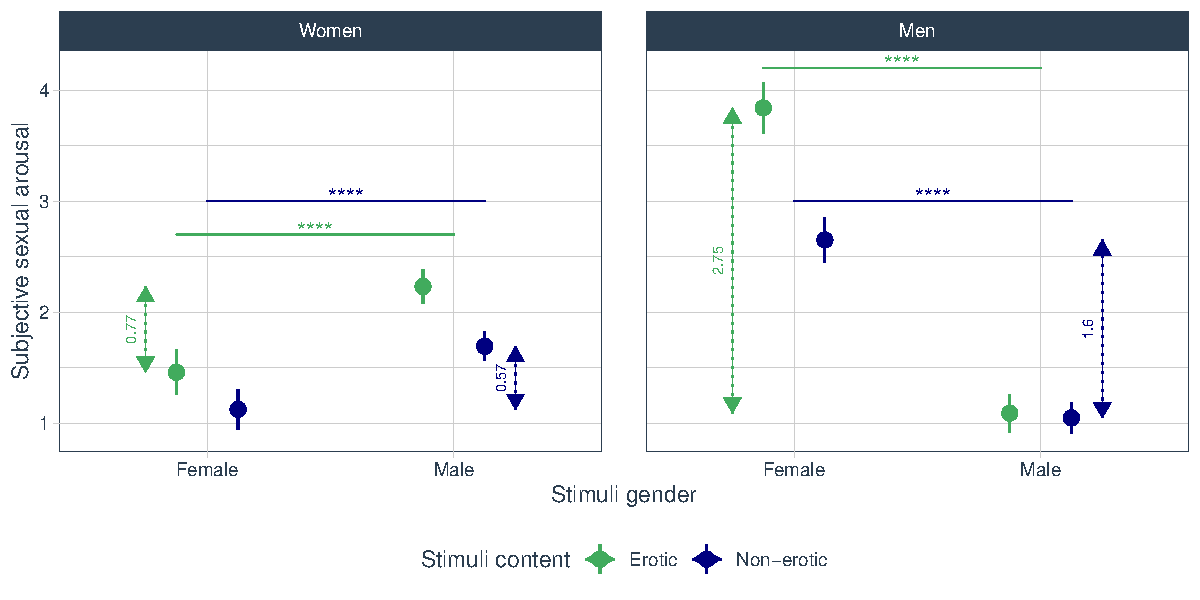
\includegraphics{Sexual_Desire_Arousal_anonymous_files/figure-latex/fig-m-stimuli-content-1.pdf}
\caption{\label{fig:fig-m-stimuli-content}Effects of stimuli content (erotic, non-erotic) on subjective sexual arousal for women's (left panel) and men's (right panel) scores of male and female stimuli (see Table \ref{tab:tab-m-stimuli-content}; for detailed results, see Table \ref{tab:tab-stim-cont-emms}). Dots and bars represent estimated marginal means and 95\% CI. Vertical lines with arrow heads represent the (absolute) difference in reported subjective sexual arousal for male and femnale stimuli, by stimuli content and gender. In all cases, significant effects are represented with lines and stars: *\emph{p} \textless{} 0.05, **\emph{p} \textless{} 0.01, ***\emph{p} \textless{} 0.001, ****\emph{p} \textless{} 0.0001.}
\end{figure}

\subsection{Hypothesis 2: The association between trait sexual desire (TSD) and subjective sexual arousal (SSA) will vary by TSD dimension, with these associations being gender-specific in men and gender-non-specific in women.}\label{hyp2}

We tested whether the relationship between SSA and TSD varies across the three dimensions of TSD and whether these associations differ between men and women. Specifically, we examined:

\begin{itemize}
\tightlist
\item
  \textbf{H2a}: A significant association between solitary TSD and SSA toward erotic stimuli (section \ref{hyp2a})
\item
  \textbf{H2b}: A significant association between dyadic TSD toward an attractive person and SSA toward erotic stimuli.
\item
  \textbf{H2c}: No significant association between dyadic TSD toward a partner and SSA toward erotic stimuli.
\end{itemize}

To examine this hypothesis, we modeled the effects of each of the three TSD dimension scores, gender, stimulus sex, and their interactions, on SSA. We included random intercepts for each stimulus, as well as random intercepts and slopes between stimuli sex for each participant.

\subsubsection{Modeling Approach}\label{modeling-approach}

Since SSA is an ordinal variable with seven ordered levels, we fitted the models using three different approaches to ensure the robustness of our results:

\begin{enumerate}
\def\labelenumi{\arabic{enumi}.}
\tightlist
\item
  Cumulative Link Mixed Model (CLMM), using the \texttt{clmm} function from the package \texttt{ordinal} \autocite{ordinalcit}
\item
  Generalized Mixed Model (GLMM) with a Poisson family, using the \texttt{glmer} function from the package \texttt{lme4} \autocite{lme4cit}
\item
  Linear mixed model (LMM), using the \texttt{lmer} function from the package \texttt{lmerTest} \autocite{lmertestcit}
\end{enumerate}

The results across these models were largely consistent, indicating robustness in our findings. For clarity and interpretability, we primarily base our inferences on the LMM, as it provides the most straightforward interpretation and has a wider range of available functions in R for extracting model information.

\subsubsection{Data}\label{data-1}

We created a new dataset by selecting only responses to erotic stimuli, renaming key variables to remove spaces for compatibility with certain functions, and converting relevant variables to factors. Specifically, the Gender and Stimuli sex variables are transformed into factors, and a factor version of Subjective sexual arousal is created for use in the CLMM model.

\begin{Shaded}
\begin{Highlighting}[]
\CommentTok{\# Filter dataset to include only responses to erotic stimuli}
\NormalTok{dat\_m2 }\OtherTok{\textless{}{-}}\NormalTok{ dat }\SpecialCharTok{|\textgreater{}}
  \FunctionTok{filter}\NormalTok{(}\StringTok{\textasciigrave{}}\AttributeTok{Stimuli content}\StringTok{\textasciigrave{}} \SpecialCharTok{==} \StringTok{"Erotic"}\NormalTok{) }\SpecialCharTok{|\textgreater{}} \CommentTok{\# Select only erotic stimuli responses}
  \CommentTok{\# Rename variables to remove spaces (improves function compatibility)}
  \FunctionTok{rename}\NormalTok{(}
    \AttributeTok{Subjective.sexual.arousal =} \StringTok{\textasciigrave{}}\AttributeTok{Subjective sexual arousal}\StringTok{\textasciigrave{}}\NormalTok{,}
    \AttributeTok{Solitary.TSD =} \StringTok{\textasciigrave{}}\AttributeTok{Solitary sexual desire}\StringTok{\textasciigrave{}}\NormalTok{,}
    \AttributeTok{Dyadic.TSD.Attractive.Person =} \StringTok{\textasciigrave{}}\AttributeTok{Dyadic sexual desire (Attractive person)}\StringTok{\textasciigrave{}}\NormalTok{,}
    \AttributeTok{Dyadic.TSD.Partner =} \StringTok{\textasciigrave{}}\AttributeTok{Dyadic sexual desire (Partner)}\StringTok{\textasciigrave{}}\NormalTok{,}
    \AttributeTok{Stimuli.sex =} \StringTok{\textasciigrave{}}\AttributeTok{Stimuli sex}\StringTok{\textasciigrave{}}\NormalTok{,}
    \AttributeTok{Stimuli.code =} \StringTok{\textasciigrave{}}\AttributeTok{Stimuli code}\StringTok{\textasciigrave{}}
\NormalTok{  ) }\SpecialCharTok{|\textgreater{}}
  \CommentTok{\# Convert categorical variables to factors}
  \FunctionTok{mutate}\NormalTok{(}
    \AttributeTok{Gender =} \FunctionTok{as.factor}\NormalTok{(Gender), }\CommentTok{\# Convert Gender to factor}
    \AttributeTok{Stimuli.sex =} \FunctionTok{as.factor}\NormalTok{(Stimuli.sex), }\CommentTok{\# Convert Stimuli sex to factor}
    \CommentTok{\# Create a factor version of SSA for use in the CLMM model}
    \AttributeTok{Subjective.sexual.arousal.factor =} \FunctionTok{as.factor}\NormalTok{(Subjective.sexual.arousal)}
\NormalTok{  )}
\end{Highlighting}
\end{Shaded}

\subsubsection{Hypothesis 2a: Solitary TSD}\label{hyp2a}

\paragraph{Model Robustness: Examining the Effects of Solitary TSD on SSA Across Gender and Stimuli Sex}\label{model-robustness-examining-the-effects-of-solitary-tsd-on-ssa-across-gender-and-stimuli-sex}

To assess the robustness of our findings, we fitted three different models examining how Solitary TSD predicts SSA, considering variations by gender and stimuli sex:

\begin{enumerate}
\def\labelenumi{\arabic{enumi}.}
\tightlist
\item
  Cumulative Link Mixed Model (CLMM) -- \texttt{m2a\_clmm} (for ordinal outcomes, using a probit link).
\item
  Generalized Linear Mixed Model (GLMM) with Poisson family -- \texttt{m2a\_poisson} (treating SSA as a count variable).
\item
  Linear Mixed Model (LMM) -- \texttt{m2a\_lmer} (treating SSA as a continuous variable).
\end{enumerate}

\begin{Shaded}
\begin{Highlighting}[]
\CommentTok{\# Fit three different models to examine how Dyadic TSD Partner predicts SSA}
\CommentTok{\# Each model considers variations by Gender and Stimuli Sex}

\CommentTok{\# (1) Cumulative Link Mixed Model (CLMM) {-} Ordinal outcome with probit link}
\NormalTok{m2a\_clmm }\OtherTok{\textless{}{-}} \FunctionTok{clmm}\NormalTok{(}
\NormalTok{  Subjective.sexual.arousal.factor }\SpecialCharTok{\textasciitilde{}}\NormalTok{ Solitary.TSD }\SpecialCharTok{*}\NormalTok{ Gender }\SpecialCharTok{*}\NormalTok{ Stimuli.sex }\SpecialCharTok{+}
\NormalTok{    (}\DecValTok{1} \SpecialCharTok{|}\NormalTok{ Stimuli.code) }\SpecialCharTok{+} \CommentTok{\# Random intercept for Stimuli}
\NormalTok{    (}\DecValTok{1} \SpecialCharTok{+}\NormalTok{ Stimuli.sex }\SpecialCharTok{|}\NormalTok{ Participant), }\CommentTok{\# Random intercept \& slope for Stimuli sex}
  \AttributeTok{data =}\NormalTok{ dat\_m2,}
  \AttributeTok{link =} \StringTok{"probit"}\NormalTok{, }\CommentTok{\# Use probit link function for ordinal regression}
  \AttributeTok{control =} \FunctionTok{list}\NormalTok{(}\AttributeTok{method =} \StringTok{"nlminb"}\NormalTok{) }\CommentTok{\# Use \textquotesingle{}nlminb\textquotesingle{} optimizer for better convergence}
\NormalTok{)}

\CommentTok{\# (2) Generalized Linear Mixed Model (GLMM) {-} Poisson regression for count data}
\NormalTok{m2a\_poisson }\OtherTok{\textless{}{-}} \FunctionTok{glmer}\NormalTok{(}
\NormalTok{  Subjective.sexual.arousal }\SpecialCharTok{\textasciitilde{}}\NormalTok{ Solitary.TSD }\SpecialCharTok{*}\NormalTok{ Gender }\SpecialCharTok{*}\NormalTok{ Stimuli.sex }\SpecialCharTok{+}
\NormalTok{    (}\DecValTok{1} \SpecialCharTok{|}\NormalTok{ Stimuli.code) }\SpecialCharTok{+} \CommentTok{\# Random intercept for Stimuli}
\NormalTok{    (}\DecValTok{1} \SpecialCharTok{+}\NormalTok{ Stimuli.sex }\SpecialCharTok{|}\NormalTok{ Participant), }\CommentTok{\# Random intercept \& slope for Stimuli sex}
  \AttributeTok{data =}\NormalTok{ dat\_m2,}
  \AttributeTok{family =}\NormalTok{ poisson }\CommentTok{\# Poisson distribution for count data}
\NormalTok{)}

\CommentTok{\# (3) Linear Mixed Model (LMM) {-} Continuous approximation}
\NormalTok{m2a\_lmer }\OtherTok{\textless{}{-}} \FunctionTok{lmer}\NormalTok{(}
\NormalTok{  Subjective.sexual.arousal }\SpecialCharTok{\textasciitilde{}}\NormalTok{ Solitary.TSD }\SpecialCharTok{*}\NormalTok{ Gender }\SpecialCharTok{*}\NormalTok{ Stimuli.sex }\SpecialCharTok{+}
\NormalTok{    (}\DecValTok{1} \SpecialCharTok{|}\NormalTok{ Stimuli.code) }\SpecialCharTok{+} \CommentTok{\# Random intercept for Stimuli}
\NormalTok{    (}\DecValTok{1} \SpecialCharTok{+}\NormalTok{ Stimuli.sex }\SpecialCharTok{|}\NormalTok{ Participant), }\CommentTok{\# Random intercept \& slope for Stimuli sex}
  \AttributeTok{data =}\NormalTok{ dat\_m2,}
  \AttributeTok{control =} \FunctionTok{lmerControl}\NormalTok{(}\AttributeTok{optimizer =} \StringTok{"bobyqa"}\NormalTok{) }\CommentTok{\# Use \textquotesingle{}bobyqa\textquotesingle{} optimizer for stability}
\NormalTok{)}
\end{Highlighting}
\end{Shaded}

\subparagraph{Table \ref{tab:tab-robu-m2a}. ANOVA-type table of fixed effects (main effects and interactions) across the three fitted models}\label{table-reftabtab-robu-m2a.-anova-type-table-of-fixed-effects-main-effects-and-interactions-across-the-three-fitted-models}

As shown in the table below, the pattern of significant effects remains consistent across all three models, except for the main effect of gender, which is not significant in the CLMM.

\begin{Shaded}
\begin{Highlighting}[]
\CommentTok{\# Compare ANOVA{-}type tables across the three fitted models for Hypothesis 2a}
\CommentTok{\# {-} CLMM: Cumulative Link Mixed Model}
\CommentTok{\# {-} GLMM (Poisson): Generalized Linear Mixed Model}
\CommentTok{\# {-} LMM: Linear Mixed Model}
\FunctionTok{anova.comp}\NormalTok{(}
  \AttributeTok{CLMMmod =}\NormalTok{ m2a\_clmm, }\CommentTok{\# Ordinal regression model (probit link)}
  \AttributeTok{GLMERmod =}\NormalTok{ m2a\_poisson, }\CommentTok{\# Poisson regression model (count data)}
  \AttributeTok{LMERmod =}\NormalTok{ m2a\_lmer, }\CommentTok{\# Linear mixed model (continuous response)}
  \AttributeTok{hypothesis =} \StringTok{"2a"} \CommentTok{\# Label for hypothesis tracking in output}
\NormalTok{)}
\end{Highlighting}
\end{Shaded}

\begin{table}[H]
\centering
\caption{\label{tab:tab-robu-m2a}Comparison of fixed effects across the three models for Hypothesis 2a: CLMM, GLMM (Poisson), and LMM.}
\centering
\resizebox{\ifdim\width>\linewidth\linewidth\else\width\fi}{!}{
\begin{threeparttable}
\begin{tabular}[t]{lccccccccc}
\toprule
\multicolumn{1}{c}{ } & \multicolumn{3}{c}{CLMM} & \multicolumn{3}{c}{GLMER (Poisson)} & \multicolumn{3}{c}{LMM} \\
\cmidrule(l{3pt}r{3pt}){2-4} \cmidrule(l{3pt}r{3pt}){5-7} \cmidrule(l{3pt}r{3pt}){8-10}
Effect & $df$ & $\chi^2$ & $p$ & $df$ & $\chi^2$ & $p$ & $df$ & $F$ & $p$\\
\midrule
Solitary TSD & 1 & 27.377 & \textbf{< 0.0001} & 1 & 24.430 & \textbf{< 0.0001} & 1, 319 & 17.464 & \textbf{< 0.0001}\\
Gender & 1 & 0.015 & 0.9 & 1 & 7.086 & \textbf{0.0078} & 1, 319 & 8.838 & \textbf{0.0032}\\
Stimuli sex & 1 & 43.812 & \textbf{< 0.0001} & 1 & 31.553 & \textbf{< 0.0001} & 1, 369.21 & 24.715 & \textbf{< 0.0001}\\
Solitary TSD × Gender & 1 & 2.409 & 0.12 & 1 & 2.795 & 0.09 & 1, 319 & 0.852 & 0.36\\
Solitary TSD × Stimuli sex & 1 & 0.137 & 0.71 & 1 & 0.321 & 0.57 & 1, 319 & 0.024 & 0.88\\
Gender × Stimuli sex & 1 & 181.478 & \textbf{< 0.0001} & 1 & 127.568 & \textbf{< 0.0001} & 1, 319 & 74.790 & \textbf{< 0.0001}\\
Solitary TSD × Gender × Stimuli sex & 1 & 2.959 & 0.09 & 1 & 0.605 & 0.44 & 1, 319 & 1.778 & 0.18\\
\bottomrule
\end{tabular}
\begin{tablenotes}[para]
\item \textit{Note: } 
\item For CLMM and GLMER (Poisson) models, results are
              Analysis of Deviance (Type III Wald chi-square tests),
              while for LMM, results are from an Analysis of Variance
              (Type III ANOVA with Satterthwaite's method).
              Significant effects are in bold.
\end{tablenotes}
\end{threeparttable}}
\end{table}

\subparagraph{Figure \ref{fig:preds-m2a}: Model-based predictions for Hypothesis 2a.}\label{figure-reffigpreds-m2a-model-based-predictions-for-hypothesis-2a.}

This figure presents model-based predictions of subjective sexual arousal as a function of Solitary TSD, across different stimulus sexes and participant genders. The three subplots correspond to the three statistical models used for analysis: (a) Cumulative Link Mixed Model (CLMM), (b) Generalized Linear Mixed Model (GLMM, Poisson), and (c) Linear Mixed Model (LMM). Shaded areas represent 95\% confidence intervals.

\begin{Shaded}
\begin{Highlighting}[]
\CommentTok{\# CLMM Predictions: Subjective Sexual Arousal \textasciitilde{} Solitary TSD | Gender * Stimuli Sex}
\NormalTok{p\_m2a\_clmm }\OtherTok{\textless{}{-}} \FunctionTok{emmeans}\NormalTok{(m2a\_clmm, }\SpecialCharTok{\textasciitilde{}}\NormalTok{ Solitary.TSD }\SpecialCharTok{|}\NormalTok{ Gender }\SpecialCharTok{*}\NormalTok{ Stimuli.sex,}
  \AttributeTok{at =} \FunctionTok{list}\NormalTok{(}\AttributeTok{Solitary.TSD =} \FunctionTok{seq}\NormalTok{(}\DecValTok{0}\NormalTok{, }\DecValTok{31}\NormalTok{, }\AttributeTok{length.out =} \DecValTok{100}\NormalTok{)), }\CommentTok{\# Predict over range of TSD}
  \AttributeTok{mode =} \StringTok{"mean.class"} \CommentTok{\# Compute predicted mean response categories}
\NormalTok{) }\SpecialCharTok{|\textgreater{}}
  \FunctionTok{as.data.frame}\NormalTok{() }\SpecialCharTok{|\textgreater{}} \CommentTok{\# Convert predictions to dataframe}
  \FunctionTok{ggplot}\NormalTok{(}\FunctionTok{aes}\NormalTok{(}
    \AttributeTok{x =}\NormalTok{ Solitary.TSD, }\AttributeTok{y =}\NormalTok{ mean.class,}
    \AttributeTok{color =}\NormalTok{ Stimuli.sex, }\AttributeTok{fill =}\NormalTok{ Stimuli.sex}
\NormalTok{  )) }\SpecialCharTok{+}
  \FunctionTok{geom\_line}\NormalTok{(}\AttributeTok{size =} \DecValTok{1}\NormalTok{) }\SpecialCharTok{+} \CommentTok{\# Add prediction lines}
  \FunctionTok{geom\_ribbon}\NormalTok{(}\FunctionTok{aes}\NormalTok{(}\AttributeTok{ymin =}\NormalTok{ asymp.LCL, }\AttributeTok{ymax =}\NormalTok{ asymp.UCL, }\AttributeTok{fill =}\NormalTok{ Stimuli.sex),}
    \AttributeTok{alpha =} \FloatTok{0.2}\NormalTok{, }\AttributeTok{color =} \ConstantTok{NA}
\NormalTok{  ) }\SpecialCharTok{+} \CommentTok{\# Add confidence interval shading}
  \FunctionTok{scale\_color\_manual}\NormalTok{(}\AttributeTok{values =}\NormalTok{ color.StimuliSex) }\SpecialCharTok{+}
  \FunctionTok{scale\_fill\_manual}\NormalTok{(}\AttributeTok{values =}\NormalTok{ color.StimuliSex) }\SpecialCharTok{+}
  \FunctionTok{facet\_wrap}\NormalTok{(}\SpecialCharTok{\textasciitilde{}}\NormalTok{Gender, }\AttributeTok{ncol =} \DecValTok{1}\NormalTok{) }\SpecialCharTok{+} \CommentTok{\# Separate plots by Gender}
  \FunctionTok{labs}\NormalTok{(}
    \AttributeTok{y =} \StringTok{"Predicted SSA"}\NormalTok{, }\AttributeTok{x =} \StringTok{"Solitary TSD"}\NormalTok{, }\AttributeTok{title =} \StringTok{"CLMM"}\NormalTok{,}
    \AttributeTok{color =} \StringTok{"Stimuli Sex"}\NormalTok{, }\AttributeTok{fill =} \StringTok{"Stimuli Sex"}
\NormalTok{  ) }\SpecialCharTok{+}
  \FunctionTok{theme\_tq}\NormalTok{() }\SpecialCharTok{+}
  \FunctionTok{theme}\NormalTok{(}\AttributeTok{legend.position =} \StringTok{"bottom"}\NormalTok{) }\SpecialCharTok{+}
  \FunctionTok{ylim}\NormalTok{(}\FunctionTok{c}\NormalTok{(}\FloatTok{0.3}\NormalTok{, }\FloatTok{5.3}\NormalTok{)) }\CommentTok{\# Set Y{-}axis limits}

\CommentTok{\# Poisson GLMM Predictions}
\NormalTok{p\_m2a\_poisson }\OtherTok{\textless{}{-}} \FunctionTok{emmeans}\NormalTok{(m2a\_poisson, }\SpecialCharTok{\textasciitilde{}}\NormalTok{ Solitary.TSD }\SpecialCharTok{|}\NormalTok{ Gender }\SpecialCharTok{*}\NormalTok{ Stimuli.sex,}
  \AttributeTok{at =} \FunctionTok{list}\NormalTok{(}\AttributeTok{Solitary.TSD =} \FunctionTok{seq}\NormalTok{(}\DecValTok{0}\NormalTok{, }\DecValTok{31}\NormalTok{, }\AttributeTok{length.out =} \DecValTok{100}\NormalTok{)),}
  \AttributeTok{type =} \StringTok{"response"} \CommentTok{\# Compute response{-}scale predictions}
\NormalTok{) }\SpecialCharTok{|\textgreater{}}
  \FunctionTok{as.data.frame}\NormalTok{() }\SpecialCharTok{|\textgreater{}}
  \FunctionTok{ggplot}\NormalTok{(}\FunctionTok{aes}\NormalTok{(}
    \AttributeTok{x =}\NormalTok{ Solitary.TSD, }\AttributeTok{y =}\NormalTok{ rate,}
    \AttributeTok{color =}\NormalTok{ Stimuli.sex, }\AttributeTok{fill =}\NormalTok{ Stimuli.sex}
\NormalTok{  )) }\SpecialCharTok{+}
  \FunctionTok{geom\_line}\NormalTok{(}\AttributeTok{size =} \DecValTok{1}\NormalTok{) }\SpecialCharTok{+}
  \FunctionTok{geom\_ribbon}\NormalTok{(}\FunctionTok{aes}\NormalTok{(}\AttributeTok{ymin =}\NormalTok{ asymp.LCL, }\AttributeTok{ymax =}\NormalTok{ asymp.UCL, }\AttributeTok{fill =}\NormalTok{ Stimuli.sex),}
    \AttributeTok{alpha =} \FloatTok{0.2}\NormalTok{, }\AttributeTok{color =} \ConstantTok{NA}
\NormalTok{  ) }\SpecialCharTok{+}
  \FunctionTok{scale\_color\_manual}\NormalTok{(}\AttributeTok{values =}\NormalTok{ color.StimuliSex) }\SpecialCharTok{+}
  \FunctionTok{scale\_fill\_manual}\NormalTok{(}\AttributeTok{values =}\NormalTok{ color.StimuliSex) }\SpecialCharTok{+}
  \FunctionTok{facet\_wrap}\NormalTok{(}\SpecialCharTok{\textasciitilde{}}\NormalTok{Gender, }\AttributeTok{ncol =} \DecValTok{1}\NormalTok{) }\SpecialCharTok{+}
  \FunctionTok{labs}\NormalTok{(}
    \AttributeTok{y =} \StringTok{""}\NormalTok{, }\AttributeTok{x =} \StringTok{"Solitary TSD"}\NormalTok{, }\AttributeTok{title =} \StringTok{"GLMER (Poisson)"}\NormalTok{,}
    \AttributeTok{color =} \StringTok{"Stimuli Sex"}\NormalTok{, }\AttributeTok{fill =} \StringTok{"Stimuli Sex"}
\NormalTok{  ) }\SpecialCharTok{+}
  \FunctionTok{theme\_tq}\NormalTok{() }\SpecialCharTok{+}
  \FunctionTok{theme}\NormalTok{(}\AttributeTok{legend.position =} \StringTok{"bottom"}\NormalTok{) }\SpecialCharTok{+}
  \FunctionTok{ylim}\NormalTok{(}\FunctionTok{c}\NormalTok{(}\FloatTok{0.3}\NormalTok{, }\FloatTok{5.3}\NormalTok{))}

\CommentTok{\# LMM Predictions}
\NormalTok{p\_m2a\_lmer }\OtherTok{\textless{}{-}} \FunctionTok{emmeans}\NormalTok{(m2a\_lmer, }\SpecialCharTok{\textasciitilde{}}\NormalTok{ Solitary.TSD }\SpecialCharTok{|}\NormalTok{ Gender }\SpecialCharTok{*}\NormalTok{ Stimuli.sex,}
  \AttributeTok{at =} \FunctionTok{list}\NormalTok{(}\AttributeTok{Solitary.TSD =} \FunctionTok{seq}\NormalTok{(}\DecValTok{0}\NormalTok{, }\DecValTok{31}\NormalTok{, }\AttributeTok{length.out =} \DecValTok{100}\NormalTok{)),}
  \AttributeTok{type =} \StringTok{"response"}
\NormalTok{) }\SpecialCharTok{|\textgreater{}}
  \FunctionTok{as.data.frame}\NormalTok{() }\SpecialCharTok{|\textgreater{}}
  \FunctionTok{ggplot}\NormalTok{(}\FunctionTok{aes}\NormalTok{(}
    \AttributeTok{x =}\NormalTok{ Solitary.TSD, }\AttributeTok{y =}\NormalTok{ emmean,}
    \AttributeTok{color =}\NormalTok{ Stimuli.sex, }\AttributeTok{fill =}\NormalTok{ Stimuli.sex}
\NormalTok{  )) }\SpecialCharTok{+}
  \FunctionTok{geom\_line}\NormalTok{(}\AttributeTok{size =} \DecValTok{1}\NormalTok{) }\SpecialCharTok{+}
  \FunctionTok{geom\_ribbon}\NormalTok{(}\FunctionTok{aes}\NormalTok{(}\AttributeTok{ymin =}\NormalTok{ asymp.LCL, }\AttributeTok{ymax =}\NormalTok{ asymp.UCL, }\AttributeTok{fill =}\NormalTok{ Stimuli.sex),}
    \AttributeTok{alpha =} \FloatTok{0.2}\NormalTok{, }\AttributeTok{color =} \ConstantTok{NA}
\NormalTok{  ) }\SpecialCharTok{+}
  \FunctionTok{scale\_color\_manual}\NormalTok{(}\AttributeTok{values =}\NormalTok{ color.StimuliSex) }\SpecialCharTok{+}
  \FunctionTok{scale\_fill\_manual}\NormalTok{(}\AttributeTok{values =}\NormalTok{ color.StimuliSex) }\SpecialCharTok{+}
  \FunctionTok{facet\_wrap}\NormalTok{(}\SpecialCharTok{\textasciitilde{}}\NormalTok{Gender, }\AttributeTok{ncol =} \DecValTok{1}\NormalTok{) }\SpecialCharTok{+}
  \FunctionTok{labs}\NormalTok{(}
    \AttributeTok{y =} \StringTok{""}\NormalTok{, }\AttributeTok{x =} \StringTok{"Solitary TSD"}\NormalTok{, }\AttributeTok{title =} \StringTok{"LMM"}\NormalTok{,}
    \AttributeTok{color =} \StringTok{"Stimuli Sex"}\NormalTok{, }\AttributeTok{fill =} \StringTok{"Stimuli Sex"}
\NormalTok{  ) }\SpecialCharTok{+}
  \FunctionTok{theme\_tq}\NormalTok{() }\SpecialCharTok{+}
  \FunctionTok{theme}\NormalTok{(}\AttributeTok{legend.position =} \StringTok{"bottom"}\NormalTok{) }\SpecialCharTok{+}
  \FunctionTok{ylim}\NormalTok{(}\FunctionTok{c}\NormalTok{(}\FloatTok{0.3}\NormalTok{, }\FloatTok{5.3}\NormalTok{))}

\CommentTok{\# Arrange all plots into a single figure}
\NormalTok{p\_robu\_m2a }\OtherTok{\textless{}{-}} \FunctionTok{ggarrange}\NormalTok{(p\_m2a\_clmm, p\_m2a\_poisson, p\_m2a\_lmer,}
  \AttributeTok{common.legend =} \ConstantTok{TRUE}\NormalTok{, }\CommentTok{\# Share legend across plots}
  \AttributeTok{labels =} \StringTok{"auto"}\NormalTok{, }\CommentTok{\# Automatically label subfigures (a, b, c)}
  \AttributeTok{legend =} \StringTok{"bottom"}\NormalTok{,}
  \AttributeTok{nrow =} \DecValTok{1} \CommentTok{\# Arrange plots in a single row}
\NormalTok{)}

\CommentTok{\# Display the combined figure}
\NormalTok{p\_robu\_m2a}
\end{Highlighting}
\end{Shaded}

\begin{figure}
\centering
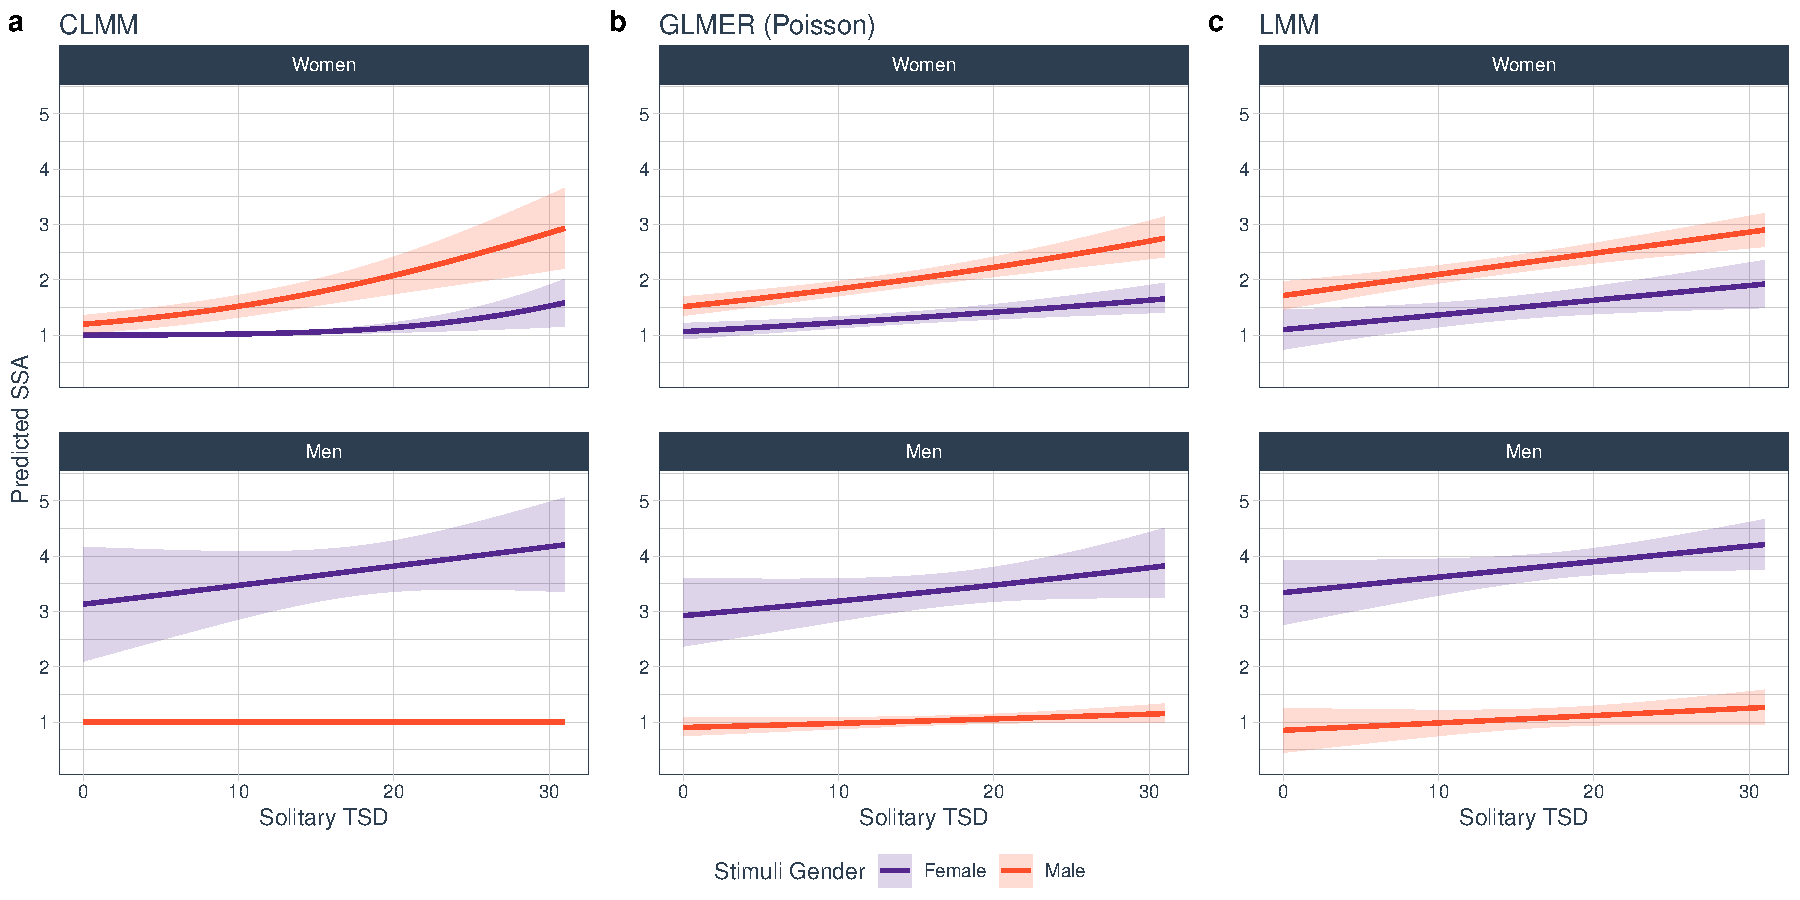
\includegraphics{Sexual_Desire_Arousal_anonymous_files/figure-latex/preds-m2a-1.pdf}
\caption{\label{fig:preds-m2a}Predicted subjective sexual arousal as a function of Solitary TSD, modeled using three statistical approaches: \textbf{(a)} Cumulative Link Mixed Model (CLMM); \textbf{(b)} Generalized Linear Mixed Model (GLMM) with a Poisson family; \textbf{(c)} Linear Mixed Model (LMM). Lines represent predicted values, and shaded areas indicate 95\% confidence intervals. The models include participant gender and stimulus sex as key factors.}
\end{figure}

\paragraph{Final Model: Effects of Solitary TSD on SSA Across Gender and Stimuli Sex}\label{final-model-effects-of-solitary-tsd-on-ssa-across-gender-and-stimuli-sex}

Given the apparent robustness of most results across models (CLMM, GLMER and LMM; Table \ref{tab:tab-robu-m2a}, Fig. \ref{fig:preds-m2a}), we test the predictions of the hypothesis from the LMM (\texttt{m2a\_lmer}).

\subparagraph{\texorpdfstring{Table \ref{tab:tab-m2a}. ANOVA-type table for the interaction between \texttt{Relationship\ type}, and \texttt{Gender}}{Table \ref{tab:tab-m2a}. ANOVA-type table for the interaction between Relationship type, and Gender}}\label{table-reftabtab-m2a.-anova-type-table-for-the-interaction-between-relationship-type-and-gender}

This tables summarizes the results of the model.

\begin{Shaded}
\begin{Highlighting}[]
\CommentTok{\# Generate ANOVA{-}type table for the final LMM model}
\CommentTok{\# This summarizes the effects of Solitary TSD on SSA across Gender and Stimuli Sex}
\FunctionTok{anova.sig.lmer}\NormalTok{(}
  \AttributeTok{model =}\NormalTok{ m2a\_lmer, }\CommentTok{\# Use LMM as the final model}
  \AttributeTok{custom\_caption =} \StringTok{"Effects of Solitary TSD on SSA Across Gender and Stimuli Sex"}
\NormalTok{)}
\end{Highlighting}
\end{Shaded}

\begin{table}[H]
\centering
\caption{\label{tab:tab-m2a}Effects of Solitary TSD on SSA Across Gender and Stimuli Sex}
\centering
\resizebox{\ifdim\width>\linewidth\linewidth\else\width\fi}{!}{
\begin{threeparttable}
\begin{tabular}[t]{lcccc}
\toprule
Effect & $df$ & $F$ & $p$ & $\epsilon^2_p$\\
\midrule
Solitary TSD & 1, 319 & 17.46 & \textbf{< 0.0001} & 0.0489\\
Gender & 1, 319 & 8.84 & \textbf{0.0032} & 0.0239\\
Stimuli sex & 1, 369.21 & 24.71 & \textbf{< 0.0001} & 0.06\\
Solitary TSD × Gender & 1, 319 & 0.85 & 0.36 & < 0.0001\\
Solitary TSD × Stimuli sex & 1, 319 & 0.02 & 0.88 & < 0.0001\\
Gender × Stimuli sex & 1, 319 & 74.79 & \textbf{< 0.0001} & 0.19\\
Solitary TSD × Gender × Stimuli sex & 1, 319 & 1.78 & 0.18 & 0.0024\\
\bottomrule
\end{tabular}
\begin{tablenotes}[para]
\item \textit{Note: } 
\item Results are Type III ANOVA. $R^2_{conditional}$ = 0.745, $R^2_{marginal}$ = 0.335. As effect size, we report partial epsilon squared ($\epsilon^2_p$), a less biased estimate than $\eta^2$ (see \cite{albersWhenPowerAnalyses2018}). Significant effects are in bold.
\end{tablenotes}
\end{threeparttable}}
\end{table}

\subparagraph{\texorpdfstring{\emph{Post-hoc} tests}{Post-hoc tests}}\label{post-hoc-tests}

To test the hypothesis, which predicted that there would be different relationship between SSA and solitary TSD, and that this association differ between men and women depending on the sex of stimuli, we used simple slope analysis.

\begin{Shaded}
\begin{Highlighting}[]
\CommentTok{\# Perform simple slopes analysis for Solitary TSD on SSA}
\CommentTok{\# Moderators: Stimuli Sex \& Gender}
\NormalTok{slop.m2a\_lmer }\OtherTok{\textless{}{-}} \FunctionTok{sim\_slopes}\NormalTok{(m2a\_lmer,}
  \AttributeTok{pred =}\NormalTok{ Solitary.TSD, }\CommentTok{\# Predictor: Solitary TSD}
  \AttributeTok{modx =}\NormalTok{ Stimuli.sex, }\CommentTok{\# First moderator: Stimuli sex}
  \AttributeTok{mod2 =}\NormalTok{ Gender, }\CommentTok{\# Second moderator: Gender}
  \AttributeTok{confint =} \ConstantTok{TRUE} \CommentTok{\# Compute confidence intervals}
\NormalTok{)}

\CommentTok{\# Extract slopes separately for Women and Men}
\NormalTok{slop.m2a\_lmer.tab }\OtherTok{\textless{}{-}} \FunctionTok{bind\_rows}\NormalTok{(}
\NormalTok{  slop.m2a\_lmer}\SpecialCharTok{$}\NormalTok{slopes[[}\DecValTok{1}\NormalTok{]] }\SpecialCharTok{|\textgreater{}} \FunctionTok{mutate}\NormalTok{(}\AttributeTok{Gender =} \StringTok{"Women"}\NormalTok{),}
\NormalTok{  slop.m2a\_lmer}\SpecialCharTok{$}\NormalTok{slopes[[}\DecValTok{2}\NormalTok{]] }\SpecialCharTok{|\textgreater{}} \FunctionTok{mutate}\NormalTok{(}\AttributeTok{Gender =} \StringTok{"Men"}\NormalTok{)}
\NormalTok{) }\SpecialCharTok{|\textgreater{}}
  \CommentTok{\# Recode Gender labels}
  \FunctionTok{mutate}\NormalTok{(}\AttributeTok{Gender =} \FunctionTok{recode\_factor}\NormalTok{(Gender, }\AttributeTok{Femenino =} \StringTok{"Women"}\NormalTok{, }\AttributeTok{Masculino =} \StringTok{"Men"}\NormalTok{)) }\SpecialCharTok{|\textgreater{}}
  \CommentTok{\# Select relevant columns and convert numeric values}
  \FunctionTok{select}\NormalTok{(}\DecValTok{8}\NormalTok{, }\DecValTok{1}\SpecialCharTok{:}\DecValTok{2}\NormalTok{, }\DecValTok{4}\SpecialCharTok{:}\DecValTok{7}\NormalTok{) }\SpecialCharTok{|\textgreater{}}
  \FunctionTok{mutate}\NormalTok{(}\FunctionTok{across}\NormalTok{(}\DecValTok{3}\SpecialCharTok{:}\DecValTok{7}\NormalTok{, as.numeric)) }\SpecialCharTok{|\textgreater{}}
  \FunctionTok{mutate}\NormalTok{(}\FunctionTok{across}\NormalTok{(}\DecValTok{3}\SpecialCharTok{:}\DecValTok{6}\NormalTok{, round, }\DecValTok{2}\NormalTok{)) }\SpecialCharTok{|\textgreater{}} \CommentTok{\# Round confidence intervals}
  \FunctionTok{mutate}\NormalTok{(}\AttributeTok{sig =} \FunctionTok{pval.stars}\NormalTok{(p)) }\SpecialCharTok{|\textgreater{}} \CommentTok{\# Convert p{-}values to significance stars}
  \FunctionTok{rename}\NormalTok{(}\StringTok{"Stimuli.sex"} \OtherTok{=} \StringTok{"Value of Stimuli.sex"}\NormalTok{) }\SpecialCharTok{|\textgreater{}}
  \FunctionTok{rename}\NormalTok{(}\AttributeTok{Coefficient =}\NormalTok{ Est.)}

\CommentTok{\# Format the table output}
\NormalTok{slop.m2a\_lmer.tab[, }\SpecialCharTok{{-}}\FunctionTok{c}\NormalTok{(}\DecValTok{1}\NormalTok{, }\DecValTok{8}\NormalTok{)] }\SpecialCharTok{|\textgreater{}}
  \FunctionTok{mutate}\NormalTok{(}\AttributeTok{p =} \FunctionTok{pval.lev}\NormalTok{(p)) }\SpecialCharTok{|\textgreater{}} \CommentTok{\# Format p{-}values}
  \FunctionTok{kable}\NormalTok{(}
    \AttributeTok{booktabs =} \ConstantTok{TRUE}\NormalTok{, }\AttributeTok{align =} \FunctionTok{c}\NormalTok{(}\StringTok{"l"}\NormalTok{, }\FunctionTok{rep}\NormalTok{(}\StringTok{"c"}\NormalTok{, }\DecValTok{5}\NormalTok{)), }
    \AttributeTok{linesep =} \StringTok{""}\NormalTok{,}
    \AttributeTok{caption =} \StringTok{"Slope for Solitary TSD on Subjective Sexual Arousal by Stimuli Sex and Gender"}\NormalTok{,}
    \AttributeTok{col.names =} \FunctionTok{c}\NormalTok{(}\StringTok{"Stimuli sex"}\NormalTok{, }\StringTok{"$B$"}\NormalTok{, }\StringTok{"$2.5}\SpecialCharTok{\textbackslash{}\textbackslash{}}\StringTok{\% CI$"}\NormalTok{, }\StringTok{"$97.5}\SpecialCharTok{\textbackslash{}\textbackslash{}}\StringTok{\% CI$"}\NormalTok{, }\StringTok{"$t$"}\NormalTok{, }\StringTok{"$p$"}\NormalTok{),}
    \AttributeTok{escape =} \ConstantTok{FALSE}
\NormalTok{  ) }\SpecialCharTok{|\textgreater{}}
  \FunctionTok{kable\_styling}\NormalTok{(}\AttributeTok{latex\_options =} \FunctionTok{c}\NormalTok{(}\StringTok{"HOLD\_position"}\NormalTok{)) }\SpecialCharTok{|\textgreater{}}
  \CommentTok{\# Add row grouping for gender}
  \FunctionTok{pack\_rows}\NormalTok{(}\StringTok{"Gender: Women"}\NormalTok{, }\AttributeTok{start\_row =} \DecValTok{1}\NormalTok{, }\AttributeTok{end\_row =} \DecValTok{2}\NormalTok{, }
            \AttributeTok{bold =} \ConstantTok{FALSE}\NormalTok{, }\AttributeTok{background =} \StringTok{"lightgray"}\NormalTok{) }\SpecialCharTok{|\textgreater{}}
  \FunctionTok{pack\_rows}\NormalTok{(}\StringTok{"Gender: Men"}\NormalTok{, }\AttributeTok{start\_row =} \DecValTok{3}\NormalTok{, }\AttributeTok{end\_row =} \DecValTok{4}\NormalTok{, }
            \AttributeTok{bold =} \ConstantTok{FALSE}\NormalTok{, }\AttributeTok{background =} \StringTok{"lightgray"}\NormalTok{) }\SpecialCharTok{|\textgreater{}}
  \CommentTok{\# Add footnote explaining coefficients}
  \FunctionTok{footnote}\NormalTok{(}
    \AttributeTok{general =} \StringTok{"$B$ are unstandardized coefficients.}
\StringTok{    No intercept is reported as continuous predictors were centered}
\StringTok{    and are dependent on this specific sample."}\NormalTok{,}
    \AttributeTok{threeparttable =} \ConstantTok{TRUE}\NormalTok{, }\AttributeTok{footnote\_as\_chunk =} \ConstantTok{TRUE}\NormalTok{, }\AttributeTok{escape =} \ConstantTok{FALSE}
\NormalTok{  )}
\end{Highlighting}
\end{Shaded}

\begin{table}[H]
\centering
\caption{\label{tab:unnamed-chunk-21}Slope for Solitary TSD on Subjective Sexual Arousal by Stimuli Sex and Gender}
\centering
\begin{threeparttable}
\begin{tabular}[t]{lccccc}
\toprule
Stimuli sex & $B$ & $2.5\% CI$ & $97.5\% CI$ & $t$ & $p$\\
\midrule
\addlinespace[0.3em]
\multicolumn{6}{l}{\cellcolor{lightgray}{Gender: Women}}\\
\hspace{1em}Female & 0.03 & 0.01 & 0.05 & 2.42 & \textbf{0.0162}\\
\hspace{1em}Male & 0.04 & 0.02 & 0.05 & 5.07 & \textbf{< 0.0001}\\
\addlinespace[0.3em]
\multicolumn{6}{l}{\cellcolor{lightgray}{Gender: Men}}\\
\hspace{1em}Female & 0.03 & 0.00 & 0.06 & 1.84 & 0.07\\
\hspace{1em}Male & 0.01 & -0.01 & 0.03 & 1.28 & 0.2\\
\bottomrule
\end{tabular}
\begin{tablenotes}[para]
\item \textit{Note: } 
\item $B$ are unstandardized coefficients.
    No intercept is reported as continuous predictors were centered
    and are dependent on this specific sample.
\end{tablenotes}
\end{threeparttable}
\end{table}

\paragraph{Figure \ref{fig:fig-h2a}. Subjective sexual arousal to erotic stimuli: Main effects and interactions}\label{figure-reffigfig-h2a.-subjective-sexual-arousal-to-erotic-stimuli-main-effects-and-interactions}

This figure summarizes the results of hypothesis 2a.

\begin{Shaded}
\begin{Highlighting}[]
\CommentTok{\# Modify LMM plot to visualize main effects \& interactions}
\NormalTok{p\_m2a.fin }\OtherTok{\textless{}{-}}\NormalTok{ p\_m2a\_lmer }\SpecialCharTok{+}
  \FunctionTok{labs}\NormalTok{(}
    \AttributeTok{title =} \StringTok{""}\NormalTok{, }\CommentTok{\# Remove title}
    \AttributeTok{y =} \StringTok{"Predicted Subjective Sexual Arousal"}
\NormalTok{  ) }\SpecialCharTok{+} \CommentTok{\# Update y{-}axis label}
  \FunctionTok{facet\_wrap}\NormalTok{(}\SpecialCharTok{\textasciitilde{}}\NormalTok{Gender, }\AttributeTok{ncol =} \DecValTok{2}\NormalTok{) }\SpecialCharTok{+} \CommentTok{\# Separate plots by Gender}
  \CommentTok{\# Add text labels for regression slopes (B, CI, p{-}values)}
  \FunctionTok{geom\_text}\NormalTok{(}
    \AttributeTok{data =}\NormalTok{ slop.m2a\_lmer.tab }\SpecialCharTok{|\textgreater{}}
      \FunctionTok{mutate}\NormalTok{(}\AttributeTok{Solitary.TSD =} \DecValTok{2}\NormalTok{), }\CommentTok{\# Set label position}
    \AttributeTok{mapping =} \FunctionTok{aes}\NormalTok{(}
      \AttributeTok{x =} \FunctionTok{min}\NormalTok{(Solitary.TSD), }\AttributeTok{y =} \ConstantTok{Inf}\NormalTok{,}
      \AttributeTok{label =} \FunctionTok{paste}\NormalTok{(}
        \StringTok{"B = "}\NormalTok{, Coefficient,}
        \StringTok{", IC 95\%["}\NormalTok{, }\StringTok{\textasciigrave{}}\AttributeTok{2.5\%}\StringTok{\textasciigrave{}}\NormalTok{, }\StringTok{", "}\NormalTok{, }\StringTok{\textasciigrave{}}\AttributeTok{97.5\%}\StringTok{\textasciigrave{}}\NormalTok{, }\StringTok{"], p"}\NormalTok{,}
        \FunctionTok{ifelse}\NormalTok{(}\FunctionTok{grepl}\NormalTok{(}\StringTok{"\textless{}"}\NormalTok{, }\FunctionTok{pe2.lev}\NormalTok{(p)), }\FunctionTok{pe2.lev}\NormalTok{(p),}
          \FunctionTok{paste0}\NormalTok{(}\StringTok{" = "}\NormalTok{, }\FunctionTok{pe2.lev}\NormalTok{(p))}
\NormalTok{        ),}
        \FunctionTok{ifelse}\NormalTok{(}\FunctionTok{is.na}\NormalTok{(sig), }\StringTok{""}\NormalTok{, sig)}
\NormalTok{      ),}
      \AttributeTok{vjust =} \DecValTok{2} \SpecialCharTok{+} \FunctionTok{as.numeric}\NormalTok{(}\FunctionTok{as.factor}\NormalTok{(Stimuli.sex)) }\SpecialCharTok{*} \DecValTok{2} \CommentTok{\# Stack labels}
\NormalTok{    ),}
    \AttributeTok{hjust =} \SpecialCharTok{{-}}\FloatTok{0.1}\NormalTok{, }\CommentTok{\# Align text to the left}
    \AttributeTok{show.legend =} \ConstantTok{FALSE}
\NormalTok{  ) }\SpecialCharTok{+} \CommentTok{\# Hide legend for text}
  \FunctionTok{theme}\NormalTok{(}\AttributeTok{legend.position =} \StringTok{"bottom"}\NormalTok{) }\CommentTok{\# Move legend to bottom}

\CommentTok{\# Display the final figure}
\NormalTok{p\_m2a.fin}
\end{Highlighting}
\end{Shaded}

\begin{figure}
\centering
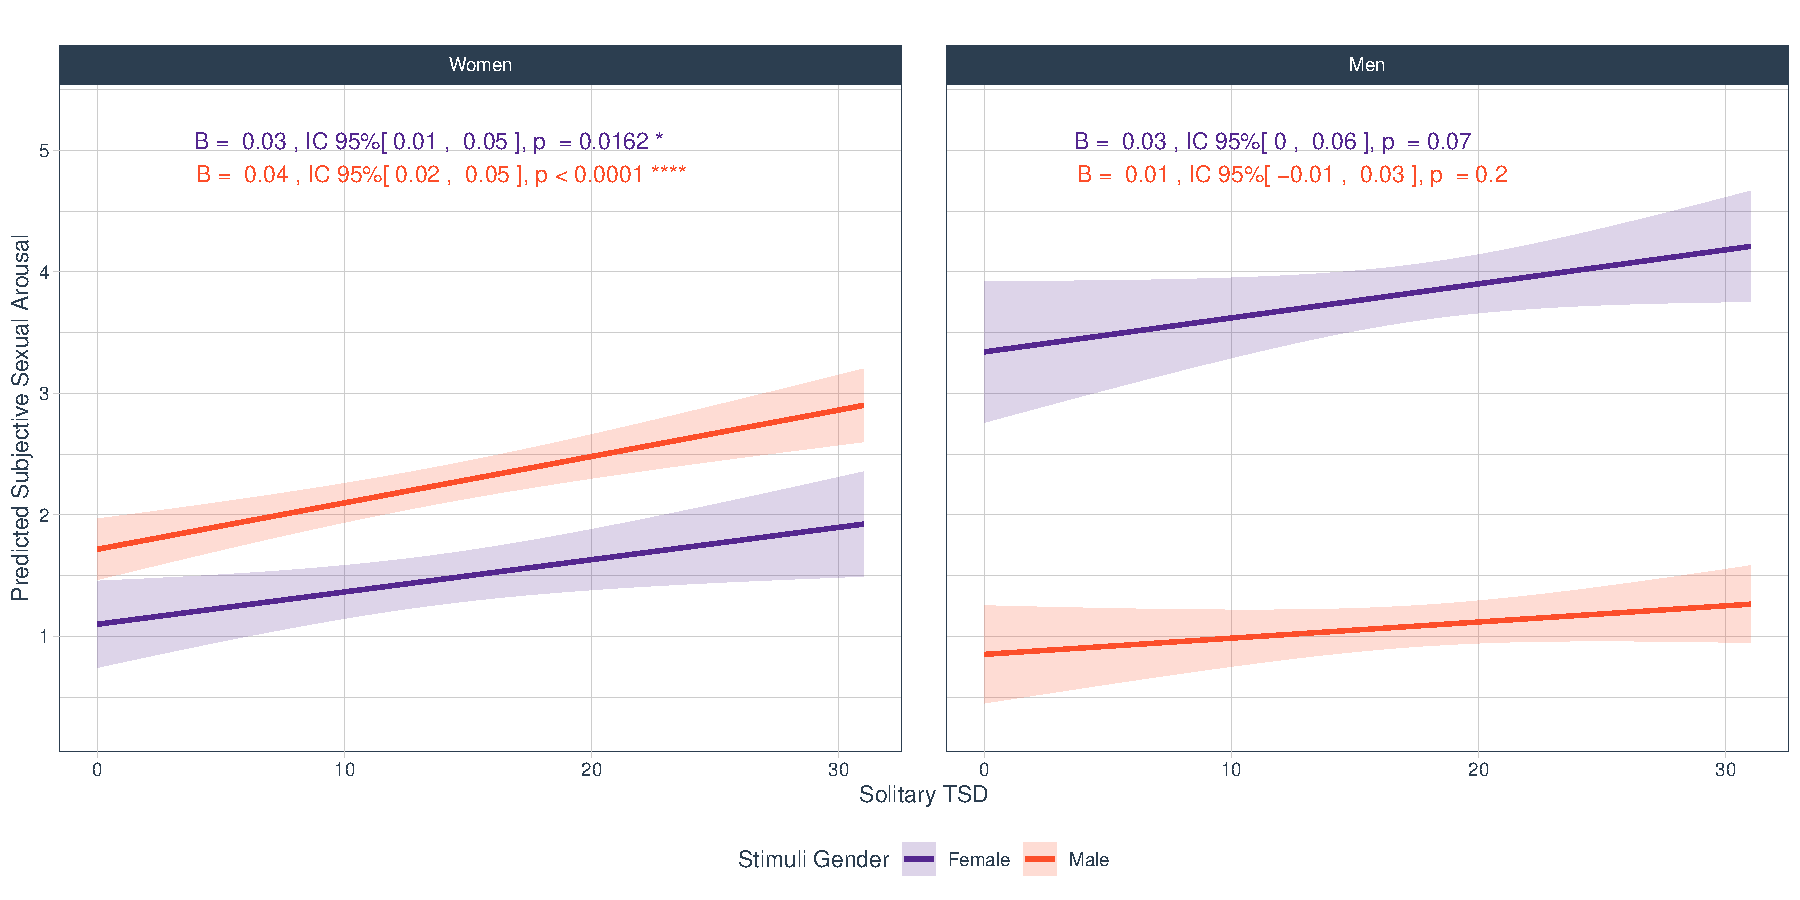
\includegraphics{Sexual_Desire_Arousal_anonymous_files/figure-latex/fig-h2a-1.pdf}
\caption{\label{fig:fig-h2a}Predicted subjective sexual arousal as a function of Solitary TSD, modeled using aLinear Mixed Model (LMM). Lines represent predicted values, and shaded areas indicate 95\% confidence intervals. The model include participant gender and stimuli sex as key factors.}
\end{figure}

\subsubsection{Hypothesis 2b: Dyadic TSD Attractive Person}\label{hyp2b}

\paragraph{Model Robustness: Examining the Effects of Dyadic TSD Attractive Person on SSA Across Gender and Stimuli Sex}\label{model-robustness-examining-the-effects-of-dyadic-tsd-attractive-person-on-ssa-across-gender-and-stimuli-sex}

To assess the robustness of our findings, we fitted three different models examining how Dyadic TSD Attractive Person predicts SSA, considering variations by gender and stimuli sex:

\begin{enumerate}
\def\labelenumi{\arabic{enumi}.}
\tightlist
\item
  Cumulative Link Mixed Model (CLMM) -- \texttt{m2b\_clmm} (for ordinal outcomes, using a probit link).
\item
  Generalized Linear Mixed Model (GLMM) with Poisson family -- \texttt{m2b\_poisson} (treating SSA as a count variable).
\item
  Linear Mixed Model (LMM) -- \texttt{m2b\_lmer} (treating SSA as a continuous variable).
\end{enumerate}

\begin{Shaded}
\begin{Highlighting}[]
\CommentTok{\# Fit three different models to examine how Dyadic TSD Partner predicts SSA}
\CommentTok{\# Each model considers variations by Gender and Stimuli Sex}

\CommentTok{\# (1) Cumulative Link Mixed Model (CLMM) {-} Ordinal outcome with probit link}
\NormalTok{m2b\_clmm }\OtherTok{\textless{}{-}} \FunctionTok{clmm}\NormalTok{(}
\NormalTok{  Subjective.sexual.arousal.factor }\SpecialCharTok{\textasciitilde{}}\NormalTok{ Dyadic.TSD.Attractive.Person }\SpecialCharTok{*}\NormalTok{ Gender }\SpecialCharTok{*}\NormalTok{ Stimuli.sex }\SpecialCharTok{+}
\NormalTok{    (}\DecValTok{1} \SpecialCharTok{|}\NormalTok{ Stimuli.code) }\SpecialCharTok{+} \CommentTok{\# Random intercept for Stimuli}
\NormalTok{    (}\DecValTok{1} \SpecialCharTok{+}\NormalTok{ Stimuli.sex }\SpecialCharTok{|}\NormalTok{ Participant), }\CommentTok{\# Random intercept \& slope for Stimuli sex}
  \AttributeTok{data =}\NormalTok{ dat\_m2,}
  \AttributeTok{link =} \StringTok{"probit"}\NormalTok{, }\CommentTok{\# Use probit link function}
  \AttributeTok{control =} \FunctionTok{list}\NormalTok{(}\AttributeTok{method =} \StringTok{"nlminb"}\NormalTok{) }\CommentTok{\# Use \textquotesingle{}nlminb\textquotesingle{} optimizer for better convergence}
\NormalTok{)}

\CommentTok{\# (2) Generalized Linear Mixed Model (GLMM) {-} Poisson regression for count data}
\NormalTok{m2b\_poisson }\OtherTok{\textless{}{-}} \FunctionTok{glmer}\NormalTok{(}
\NormalTok{  Subjective.sexual.arousal }\SpecialCharTok{\textasciitilde{}}\NormalTok{ Dyadic.TSD.Attractive.Person }\SpecialCharTok{*}\NormalTok{ Gender }\SpecialCharTok{*}\NormalTok{ Stimuli.sex }\SpecialCharTok{+}
\NormalTok{    (}\DecValTok{1} \SpecialCharTok{|}\NormalTok{ Stimuli.code) }\SpecialCharTok{+} \CommentTok{\# Random intercept for Stimuli}
\NormalTok{    (}\DecValTok{1} \SpecialCharTok{+}\NormalTok{ Stimuli.sex }\SpecialCharTok{|}\NormalTok{ Participant), }\CommentTok{\# Random intercept \& slope for Stimuli sex}
  \AttributeTok{data =}\NormalTok{ dat\_m2,}
  \AttributeTok{family =}\NormalTok{ poisson }\CommentTok{\# Use Poisson distribution for count data}
\NormalTok{)}

\CommentTok{\# (3) Linear Mixed Model (LMM) {-} Continuous approximation}
\NormalTok{m2b\_lmer }\OtherTok{\textless{}{-}} \FunctionTok{lmer}\NormalTok{(}
\NormalTok{  Subjective.sexual.arousal }\SpecialCharTok{\textasciitilde{}}\NormalTok{ Dyadic.TSD.Attractive.Person }\SpecialCharTok{*}\NormalTok{ Gender }\SpecialCharTok{*}\NormalTok{ Stimuli.sex }\SpecialCharTok{+}
\NormalTok{    (}\DecValTok{1} \SpecialCharTok{|}\NormalTok{ Stimuli.code) }\SpecialCharTok{+} \CommentTok{\# Random intercept for Stimuli}
\NormalTok{    (}\DecValTok{1} \SpecialCharTok{+}\NormalTok{ Stimuli.sex }\SpecialCharTok{|}\NormalTok{ Participant), }\CommentTok{\# Random intercept \& slope for Stimuli sex}
  \AttributeTok{data =}\NormalTok{ dat\_m2,}
  \AttributeTok{control =} \FunctionTok{lmerControl}\NormalTok{(}\AttributeTok{optimizer =} \StringTok{"bobyqa"}\NormalTok{) }\CommentTok{\# Use \textquotesingle{}bobyqa\textquotesingle{} optimizer for stability}
\NormalTok{)}
\end{Highlighting}
\end{Shaded}

\subparagraph{Table \ref{tab:tab-robu-m2b}. ANOVA-type table of fixed effects (main effects and interactions) across the three fitted models}\label{table-reftabtab-robu-m2b.-anova-type-table-of-fixed-effects-main-effects-and-interactions-across-the-three-fitted-models}

As shown in the table below, the pattern of significant effects remains consistent across all three models, except for the main effect of gender, which is not significant in the CLMM.

\begin{Shaded}
\begin{Highlighting}[]
\CommentTok{\# Compare fixed effects across the three models for Hypothesis 2b}
\CommentTok{\# CLMM: Cumulative Link Mixed Model}
\CommentTok{\# GLMER: Generalized Linear Mixed Model (Poisson)}
\CommentTok{\# LMER: Linear Mixed Model}
\FunctionTok{anova.comp}\NormalTok{(}
  \AttributeTok{CLMMmod =}\NormalTok{ m2b\_clmm, }\CommentTok{\# CLMM model}
  \AttributeTok{GLMERmod =}\NormalTok{ m2b\_poisson, }\CommentTok{\# GLMER model}
  \AttributeTok{LMERmod =}\NormalTok{ m2b\_lmer, }\CommentTok{\# LMER model}
  \AttributeTok{hypothesis =} \StringTok{"2b"} \CommentTok{\# Label hypothesis for output}
\NormalTok{)}
\end{Highlighting}
\end{Shaded}

\begin{table}[H]
\centering
\caption{\label{tab:tab-robu-m2b}Comparison of fixed effects across the three models for Hypothesis 2b: CLMM, GLMM (Poisson), and LMM.}
\centering
\resizebox{\ifdim\width>\linewidth\linewidth\else\width\fi}{!}{
\begin{threeparttable}
\begin{tabular}[t]{lccccccccc}
\toprule
\multicolumn{1}{c}{ } & \multicolumn{3}{c}{CLMM} & \multicolumn{3}{c}{GLMER (Poisson)} & \multicolumn{3}{c}{LMM} \\
\cmidrule(l{3pt}r{3pt}){2-4} \cmidrule(l{3pt}r{3pt}){5-7} \cmidrule(l{3pt}r{3pt}){8-10}
Effect & $df$ & $\chi^2$ & $p$ & $df$ & $\chi^2$ & $p$ & $df$ & $F$ & $p$\\
\midrule
Dyadic TSD Attractive Person & 1 & 36.545 & \textbf{< 0.0001} & 1 & 45.711 & \textbf{< 0.0001} & 1, 319 & 48.490 & \textbf{< 0.0001}\\
Gender & 1 & 0.031 & 0.86 & 1 & 3.059 & 0.08 & 1, 319 & 1.446 & 0.23\\
Stimuli sex & 1 & 18.293 & \textbf{< 0.0001} & 1 & 7.365 & \textbf{0.0067} & 1, 373.93 & 2.689 & 0.1\\
Dyadic TSD Attractive Person × Gender & 1 & 3.774 & 0.05 & 1 & 0.940 & 0.33 & 1, 319 & 0.530 & 0.47\\
Dyadic TSD Attractive Person × Stimuli sex & 1 & 7.654 & \textbf{0.0057} & 1 & 7.507 & \textbf{0.0061} & 1, 319 & 15.428 & \textbf{< 0.001}\\
Gender × Stimuli sex & 1 & 124.186 & \textbf{< 0.0001} & 1 & 67.054 & \textbf{< 0.0001} & 1, 319 & 27.444 & \textbf{< 0.0001}\\
Dyadic TSD Attractive Person × Gender × Stimuli sex & 1 & 3.833 & 0.05 & 1 & 20.127 & \textbf{< 0.0001} & 1, 319 & 29.689 & \textbf{< 0.0001}\\
\bottomrule
\end{tabular}
\begin{tablenotes}[para]
\item \textit{Note: } 
\item For CLMM and GLMER (Poisson) models, results are
              Analysis of Deviance (Type III Wald chi-square tests),
              while for LMM, results are from an Analysis of Variance
              (Type III ANOVA with Satterthwaite's method).
              Significant effects are in bold.
\end{tablenotes}
\end{threeparttable}}
\end{table}

\subparagraph{Figure \ref{fig:preds-m2b}: Model-based predictions for Hypothesis 2b.}\label{figure-reffigpreds-m2b-model-based-predictions-for-hypothesis-2b.}

This figure presents model-based predictions of subjective sexual arousal as a function of Dyadic TSD Attractive Person, across different stimulus sexes and participant genders. The three subplots correspond to the three statistical models used for analysis: (a) Cumulative Link Mixed Model (CLMM), (b) Generalized Linear Mixed Model (GLMM, Poisson), and (c) Linear Mixed Model (LMM). Shaded areas represent 95\% confidence intervals.

\begin{Shaded}
\begin{Highlighting}[]
\CommentTok{\# CLMM Predictions}
\NormalTok{p\_m2b\_clmm }\OtherTok{\textless{}{-}} \FunctionTok{emmeans}\NormalTok{(m2b\_clmm, }\SpecialCharTok{\textasciitilde{}}\NormalTok{ Dyadic.TSD.Attractive.Person }\SpecialCharTok{|}\NormalTok{ Gender }\SpecialCharTok{*}\NormalTok{ Stimuli.sex,}
  \AttributeTok{at =} \FunctionTok{list}\NormalTok{(}\AttributeTok{Dyadic.TSD.Attractive.Person =} \FunctionTok{seq}\NormalTok{(}\DecValTok{0}\NormalTok{, }\DecValTok{31}\NormalTok{, }\AttributeTok{length.out =} \DecValTok{100}\NormalTok{)),}
  \AttributeTok{mode =} \StringTok{"mean.class"} \CommentTok{\# Compute predicted mean response categories}
\NormalTok{) }\SpecialCharTok{|\textgreater{}}
  \FunctionTok{as.data.frame}\NormalTok{() }\SpecialCharTok{|\textgreater{}} \CommentTok{\# Convert to dataframe for ggplot}
  \FunctionTok{ggplot}\NormalTok{(}\FunctionTok{aes}\NormalTok{(}
    \AttributeTok{x =}\NormalTok{ Dyadic.TSD.Attractive.Person, }\AttributeTok{y =}\NormalTok{ mean.class,}
    \AttributeTok{color =}\NormalTok{ Stimuli.sex, }\AttributeTok{fill =}\NormalTok{ Stimuli.sex}
\NormalTok{  )) }\SpecialCharTok{+}
  \FunctionTok{geom\_line}\NormalTok{(}\AttributeTok{size =} \DecValTok{1}\NormalTok{) }\SpecialCharTok{+} \CommentTok{\# Add predicted response line}
  \FunctionTok{geom\_ribbon}\NormalTok{(}\FunctionTok{aes}\NormalTok{(}\AttributeTok{ymin =}\NormalTok{ asymp.LCL, }\AttributeTok{ymax =}\NormalTok{ asymp.UCL, }\AttributeTok{fill =}\NormalTok{ Stimuli.sex),}
    \AttributeTok{alpha =} \FloatTok{0.2}\NormalTok{, }\AttributeTok{color =} \ConstantTok{NA}
\NormalTok{  ) }\SpecialCharTok{+} \CommentTok{\# Add confidence interval as shaded ribbon}
  \FunctionTok{scale\_color\_manual}\NormalTok{(}\AttributeTok{values =}\NormalTok{ color.StimuliSex) }\SpecialCharTok{+}
  \FunctionTok{scale\_fill\_manual}\NormalTok{(}\AttributeTok{values =}\NormalTok{ color.StimuliSex) }\SpecialCharTok{+}
  \FunctionTok{facet\_wrap}\NormalTok{(}\SpecialCharTok{\textasciitilde{}}\NormalTok{Gender, }\AttributeTok{ncol =} \DecValTok{1}\NormalTok{) }\SpecialCharTok{+} \CommentTok{\# Create separate plots for each gender}
  \FunctionTok{labs}\NormalTok{(}
    \AttributeTok{y =} \StringTok{"Predicted Subjective Sexual Arousal"}\NormalTok{,}
    \AttributeTok{x =} \StringTok{"Dyadic TSD Attractive Person"}\NormalTok{,}
    \AttributeTok{title =} \StringTok{"CLMM"}\NormalTok{, }\AttributeTok{color =} \StringTok{"Stimuli Sex"}\NormalTok{, }\AttributeTok{fill =} \StringTok{"Stimuli Sex"}
\NormalTok{  ) }\SpecialCharTok{+}
  \FunctionTok{theme\_tq}\NormalTok{() }\SpecialCharTok{+}
  \FunctionTok{theme}\NormalTok{(}\AttributeTok{legend.position =} \StringTok{"bottom"}\NormalTok{) }\SpecialCharTok{+}
  \FunctionTok{ylim}\NormalTok{(}\FunctionTok{c}\NormalTok{(}\FloatTok{0.3}\NormalTok{, }\FloatTok{6.5}\NormalTok{)) }\CommentTok{\# Set Y{-}axis limits}

\CommentTok{\# Poisson GLMM Predictions}
\NormalTok{p\_m2b\_poisson }\OtherTok{\textless{}{-}} \FunctionTok{emmeans}\NormalTok{(m2b\_poisson, }\SpecialCharTok{\textasciitilde{}}\NormalTok{ Dyadic.TSD.Attractive.Person }\SpecialCharTok{|}\NormalTok{ Gender }\SpecialCharTok{*}\NormalTok{ Stimuli.sex,}
  \AttributeTok{at =} \FunctionTok{list}\NormalTok{(}\AttributeTok{Dyadic.TSD.Attractive.Person =} \FunctionTok{seq}\NormalTok{(}\DecValTok{0}\NormalTok{, }\DecValTok{31}\NormalTok{, }\AttributeTok{length.out =} \DecValTok{100}\NormalTok{)),}
  \AttributeTok{type =} \StringTok{"response"} \CommentTok{\# Compute response{-}scale predictions}
\NormalTok{) }\SpecialCharTok{|\textgreater{}}
  \FunctionTok{as.data.frame}\NormalTok{() }\SpecialCharTok{|\textgreater{}}
  \FunctionTok{ggplot}\NormalTok{(}\FunctionTok{aes}\NormalTok{(}
    \AttributeTok{x =}\NormalTok{ Dyadic.TSD.Attractive.Person, }\AttributeTok{y =}\NormalTok{ rate,}
    \AttributeTok{color =}\NormalTok{ Stimuli.sex, }\AttributeTok{fill =}\NormalTok{ Stimuli.sex}
\NormalTok{  )) }\SpecialCharTok{+}
  \FunctionTok{geom\_line}\NormalTok{(}\AttributeTok{size =} \DecValTok{1}\NormalTok{) }\SpecialCharTok{+}
  \FunctionTok{geom\_ribbon}\NormalTok{(}\FunctionTok{aes}\NormalTok{(}\AttributeTok{ymin =}\NormalTok{ asymp.LCL, }\AttributeTok{ymax =}\NormalTok{ asymp.UCL, }\AttributeTok{fill =}\NormalTok{ Stimuli.sex),}
    \AttributeTok{alpha =} \FloatTok{0.2}\NormalTok{, }\AttributeTok{color =} \ConstantTok{NA}
\NormalTok{  ) }\SpecialCharTok{+}
  \FunctionTok{scale\_color\_manual}\NormalTok{(}\AttributeTok{values =}\NormalTok{ color.StimuliSex) }\SpecialCharTok{+}
  \FunctionTok{scale\_fill\_manual}\NormalTok{(}\AttributeTok{values =}\NormalTok{ color.StimuliSex) }\SpecialCharTok{+}
  \FunctionTok{facet\_wrap}\NormalTok{(}\SpecialCharTok{\textasciitilde{}}\NormalTok{Gender, }\AttributeTok{ncol =} \DecValTok{1}\NormalTok{) }\SpecialCharTok{+}
  \FunctionTok{labs}\NormalTok{(}
    \AttributeTok{y =} \StringTok{""}\NormalTok{, }\AttributeTok{x =} \StringTok{"Dyadic TSD Attractive Person"}\NormalTok{,}
    \AttributeTok{title =} \StringTok{"GLMER (Poisson)"}\NormalTok{, }\AttributeTok{color =} \StringTok{"Stimuli Sex"}\NormalTok{, }\AttributeTok{fill =} \StringTok{"Stimuli Sex"}
\NormalTok{  ) }\SpecialCharTok{+}
  \FunctionTok{theme\_tq}\NormalTok{() }\SpecialCharTok{+}
  \FunctionTok{theme}\NormalTok{(}\AttributeTok{legend.position =} \StringTok{"bottom"}\NormalTok{) }\SpecialCharTok{+}
  \FunctionTok{ylim}\NormalTok{(}\FunctionTok{c}\NormalTok{(}\FloatTok{0.3}\NormalTok{, }\FloatTok{6.5}\NormalTok{))}

\CommentTok{\# LMM Predictions}
\NormalTok{p\_m2b\_lmer }\OtherTok{\textless{}{-}} \FunctionTok{emmeans}\NormalTok{(m2b\_lmer, }\SpecialCharTok{\textasciitilde{}}\NormalTok{ Dyadic.TSD.Attractive.Person }\SpecialCharTok{|}\NormalTok{ Gender }\SpecialCharTok{*}\NormalTok{ Stimuli.sex,}
  \AttributeTok{at =} \FunctionTok{list}\NormalTok{(}\AttributeTok{Dyadic.TSD.Attractive.Person =} \FunctionTok{seq}\NormalTok{(}\DecValTok{0}\NormalTok{, }\DecValTok{31}\NormalTok{, }\AttributeTok{length.out =} \DecValTok{100}\NormalTok{)),}
  \AttributeTok{type =} \StringTok{"response"}
\NormalTok{) }\SpecialCharTok{|\textgreater{}}
  \FunctionTok{as.data.frame}\NormalTok{() }\SpecialCharTok{|\textgreater{}}
  \FunctionTok{ggplot}\NormalTok{(}\FunctionTok{aes}\NormalTok{(}
    \AttributeTok{x =}\NormalTok{ Dyadic.TSD.Attractive.Person, }\AttributeTok{y =}\NormalTok{ emmean,}
    \AttributeTok{color =}\NormalTok{ Stimuli.sex, }\AttributeTok{fill =}\NormalTok{ Stimuli.sex}
\NormalTok{  )) }\SpecialCharTok{+}
  \FunctionTok{geom\_line}\NormalTok{(}\AttributeTok{size =} \DecValTok{1}\NormalTok{) }\SpecialCharTok{+}
  \FunctionTok{geom\_ribbon}\NormalTok{(}\FunctionTok{aes}\NormalTok{(}\AttributeTok{ymin =}\NormalTok{ asymp.LCL, }\AttributeTok{ymax =}\NormalTok{ asymp.UCL, }\AttributeTok{fill =}\NormalTok{ Stimuli.sex),}
    \AttributeTok{alpha =} \FloatTok{0.2}\NormalTok{, }\AttributeTok{color =} \ConstantTok{NA}
\NormalTok{  ) }\SpecialCharTok{+}
  \FunctionTok{scale\_color\_manual}\NormalTok{(}\AttributeTok{values =}\NormalTok{ color.StimuliSex) }\SpecialCharTok{+}
  \FunctionTok{scale\_fill\_manual}\NormalTok{(}\AttributeTok{values =}\NormalTok{ color.StimuliSex) }\SpecialCharTok{+}
  \FunctionTok{facet\_wrap}\NormalTok{(}\SpecialCharTok{\textasciitilde{}}\NormalTok{Gender, }\AttributeTok{ncol =} \DecValTok{1}\NormalTok{) }\SpecialCharTok{+}
  \FunctionTok{labs}\NormalTok{(}
    \AttributeTok{y =} \StringTok{""}\NormalTok{, }\AttributeTok{x =} \StringTok{"Dyadic TSD Attractive Person"}\NormalTok{,}
    \AttributeTok{title =} \StringTok{"LMM"}\NormalTok{, }\AttributeTok{color =} \StringTok{"Stimuli Sex"}\NormalTok{, }\AttributeTok{fill =} \StringTok{"Stimuli Sex"}
\NormalTok{  ) }\SpecialCharTok{+}
  \FunctionTok{theme\_tq}\NormalTok{() }\SpecialCharTok{+}
  \FunctionTok{theme}\NormalTok{(}\AttributeTok{legend.position =} \StringTok{"bottom"}\NormalTok{) }\SpecialCharTok{+}
  \FunctionTok{ylim}\NormalTok{(}\FunctionTok{c}\NormalTok{(}\FloatTok{0.3}\NormalTok{, }\FloatTok{6.5}\NormalTok{))}

\CommentTok{\# Arrange Plots into a Single Figure}
\NormalTok{p\_robu\_m2b }\OtherTok{\textless{}{-}} \FunctionTok{ggarrange}\NormalTok{(}
\NormalTok{  p\_m2b\_clmm, p\_m2b\_poisson, p\_m2b\_lmer, }\CommentTok{\# Combine plots side by side}
  \AttributeTok{common.legend =} \ConstantTok{TRUE}\NormalTok{, }\CommentTok{\# Share legend across plots}
  \AttributeTok{labels =} \StringTok{"auto"}\NormalTok{, }\CommentTok{\# Automatically label subfigures (a, b, c)}
  \AttributeTok{legend =} \StringTok{"bottom"}\NormalTok{,}
  \AttributeTok{nrow =} \DecValTok{1} \CommentTok{\# Arrange in a single row}
\NormalTok{)}

\CommentTok{\# Display the combined figure}
\NormalTok{p\_robu\_m2b}
\end{Highlighting}
\end{Shaded}

\begin{figure}
\centering
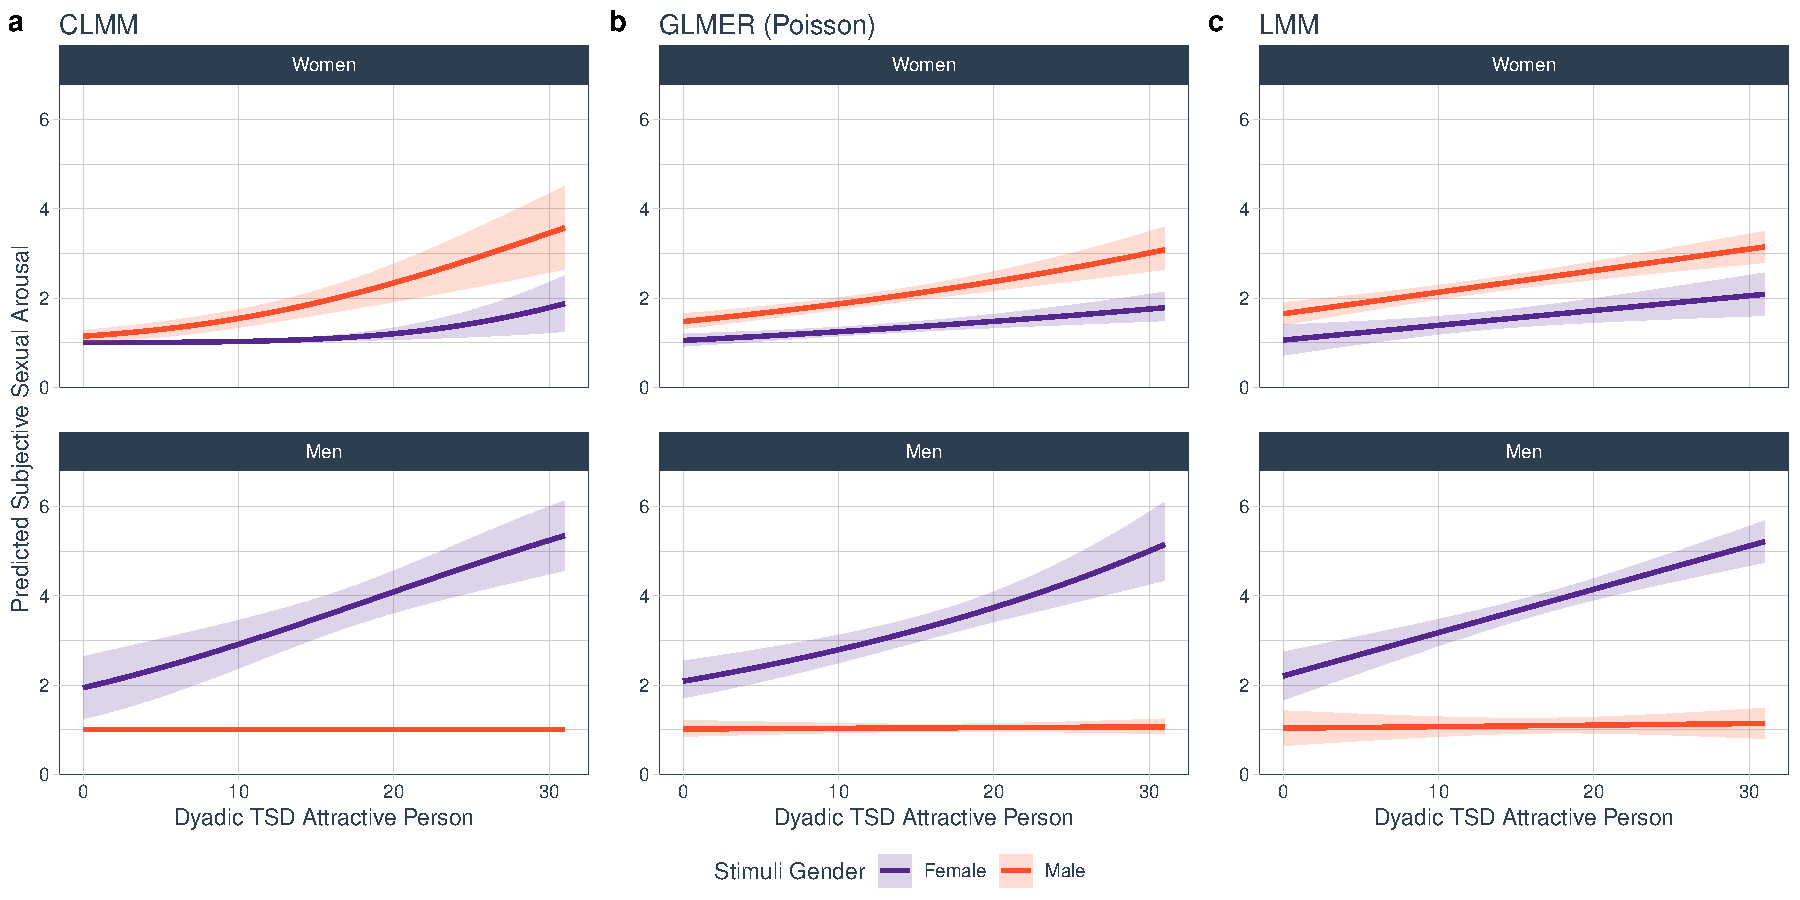
\includegraphics{Sexual_Desire_Arousal_anonymous_files/figure-latex/preds-m2b-1.pdf}
\caption{\label{fig:preds-m2b}Predicted subjective sexual arousal as a function of Dyadic TSD Attractive Person, modeled using three statistical approaches: \textbf{(a)} Cumulative Link Mixed Model (CLMM); \textbf{(b)} Generalized Linear Mixed Model (GLMM) with a Poisson family; \textbf{(c)} Linear Mixed Model (LMM). Lines represent predicted values, and shaded areas indicate 95\% confidence intervals. The models include participant gender and stimulus sex as key factors.}
\end{figure}

\paragraph{Final Model: Effects of Dyadic TSD Attractive Person on SSA Across Gender and Stimuli Sex}\label{final-model-effects-of-dyadic-tsd-attractive-person-on-ssa-across-gender-and-stimuli-sex}

Given the apparent robustness of most results across models (CLMM, GLMER and LMM; Table \ref{tab:tab-robu-m2b}, Fig. \ref{fig:preds-m2b}), we test the predictions of the hypothesis from the LMM (\texttt{m2b\_lmer}).

\subparagraph{\texorpdfstring{Table \ref{tab:tab-m2b}. ANOVA-type table for the interaction between \texttt{Relationship\ type}, and \texttt{Gender}}{Table \ref{tab:tab-m2b}. ANOVA-type table for the interaction between Relationship type, and Gender}}\label{table-reftabtab-m2b.-anova-type-table-for-the-interaction-between-relationship-type-and-gender}

This tables summarizes the results of the model.

\begin{Shaded}
\begin{Highlighting}[]
\CommentTok{\# Generate ANOVA{-}type table for the final LMM model}
\CommentTok{\# Summarizes the effects of Dyadic TSD Attractive Person on SSA across Gender and Stimuli Sex}
\FunctionTok{anova.sig.lmer}\NormalTok{(}
  \AttributeTok{model =}\NormalTok{ m2b\_lmer, }\CommentTok{\# Use LMM as the final model}
  \AttributeTok{custom\_caption =} \StringTok{"Effects of Dyadic TSD Attractive Person on SSA }
\StringTok{  Across Gender and Stimuli Sex"}
\NormalTok{)}
\end{Highlighting}
\end{Shaded}

\begin{table}[H]
\centering
\caption{\label{tab:tab-m2b}Effects of Dyadic TSD Attractive Person on SSA 
  Across Gender and Stimuli Sex}
\centering
\resizebox{\ifdim\width>\linewidth\linewidth\else\width\fi}{!}{
\begin{threeparttable}
\begin{tabular}[t]{lcccc}
\toprule
Effect & $df$ & $F$ & $p$ & $\epsilon^2_p$\\
\midrule
Dyadic TSD Attractive Person & 1, 319 & 48.49 & \textbf{< 0.0001} & 0.13\\
Gender & 1, 319 & 1.45 & 0.23 & 0.0014\\
Stimuli sex & 1, 373.93 & 2.69 & 0.1 & 0.0045\\
Dyadic TSD Attractive Person × Gender & 1, 319 & 0.53 & 0.47 & < 0.0001\\
Dyadic TSD Attractive Person × Stimuli sex & 1, 319 & 15.43 & \textbf{< 0.001} & 0.0431\\
Gender × Stimuli sex & 1, 319 & 27.44 & \textbf{< 0.0001} & 0.08\\
Dyadic TSD Attractive Person × Gender × Stimuli sex & 1, 319 & 29.69 & \textbf{< 0.0001} & 0.08\\
\bottomrule
\end{tabular}
\begin{tablenotes}[para]
\item \textit{Note: } 
\item Results are Type III ANOVA. $R^2_{conditional}$ = 0.745, $R^2_{marginal}$ = 0.367. As effect size, we report partial epsilon squared ($\epsilon^2_p$), a less biased estimate than $\eta^2$ (see \cite{albersWhenPowerAnalyses2018}). Significant effects are in bold.
\end{tablenotes}
\end{threeparttable}}
\end{table}

\subparagraph{\texorpdfstring{\emph{Post-hoc} tests}{Post-hoc tests}}\label{post-hoc-tests-1}

To test the hypothesis, which predicted that there would be different relationship between SSA and Dyadic TSD Attractive Person, and that this association differ between men and women depending on the sex of stimuli, we used simple slope analysis.

\begin{Shaded}
\begin{Highlighting}[]
\CommentTok{\# Perform simple slope analysis for Dyadic TSD Attractive Person on SSA}
\CommentTok{\# This examines differences by stimuli sex and participant gender}
\NormalTok{slop.m2b\_lmer }\OtherTok{\textless{}{-}} \FunctionTok{sim\_slopes}\NormalTok{(}
\NormalTok{  m2b\_lmer,}
  \AttributeTok{pred =}\NormalTok{ Dyadic.TSD.Attractive.Person, }\CommentTok{\# Predictor: Dyadic TSD Attractive Person}
  \AttributeTok{modx =}\NormalTok{ Stimuli.sex, }\CommentTok{\# Moderator: Stimuli sex}
  \AttributeTok{mod2 =}\NormalTok{ Gender, }\CommentTok{\# Second moderator: Gender}
  \AttributeTok{confint =} \ConstantTok{TRUE} \CommentTok{\# Compute confidence intervals}
\NormalTok{)}

\CommentTok{\# Format the slope results into a structured table}
\NormalTok{slop.m2b\_lmer.tab }\OtherTok{\textless{}{-}} \FunctionTok{bind\_rows}\NormalTok{(}
\NormalTok{  slop.m2b\_lmer}\SpecialCharTok{$}\NormalTok{slopes[[}\DecValTok{1}\NormalTok{]] }\SpecialCharTok{|\textgreater{}} \FunctionTok{mutate}\NormalTok{(}\AttributeTok{Gender =} \StringTok{"Women"}\NormalTok{),}
\NormalTok{  slop.m2b\_lmer}\SpecialCharTok{$}\NormalTok{slopes[[}\DecValTok{2}\NormalTok{]] }\SpecialCharTok{|\textgreater{}} \FunctionTok{mutate}\NormalTok{(}\AttributeTok{Gender =} \StringTok{"Men"}\NormalTok{)}
\NormalTok{) }\SpecialCharTok{|\textgreater{}}
  \FunctionTok{mutate}\NormalTok{(}\AttributeTok{Gender =} \FunctionTok{recode\_factor}\NormalTok{(Gender, }\AttributeTok{Femenino =} \StringTok{"Women"}\NormalTok{, }\AttributeTok{Masculino =} \StringTok{"Men"}\NormalTok{)) }\SpecialCharTok{|\textgreater{}}
  \FunctionTok{select}\NormalTok{(}\DecValTok{8}\NormalTok{, }\DecValTok{1}\SpecialCharTok{:}\DecValTok{2}\NormalTok{, }\DecValTok{4}\SpecialCharTok{:}\DecValTok{7}\NormalTok{) }\SpecialCharTok{|\textgreater{}}
  \FunctionTok{mutate}\NormalTok{(}\FunctionTok{across}\NormalTok{(}\DecValTok{3}\SpecialCharTok{:}\DecValTok{7}\NormalTok{, as.numeric)) }\SpecialCharTok{|\textgreater{}}
  \FunctionTok{mutate}\NormalTok{(}\FunctionTok{across}\NormalTok{(}\DecValTok{3}\SpecialCharTok{:}\DecValTok{6}\NormalTok{, round, }\DecValTok{2}\NormalTok{)) }\SpecialCharTok{|\textgreater{}}
  \FunctionTok{mutate}\NormalTok{(}\AttributeTok{sig =} \FunctionTok{pval.stars}\NormalTok{(p)) }\SpecialCharTok{|\textgreater{}}
  \FunctionTok{rename}\NormalTok{(}\StringTok{"Stimuli.sex"} \OtherTok{=} \StringTok{"Value of Stimuli.sex"}\NormalTok{, }\AttributeTok{Coefficient =}\NormalTok{ Est.)}

\CommentTok{\# Generate formatted table for slopes of Dyadic TSD Attractive Person on SSA}
\NormalTok{slop.m2b\_lmer.tab[, }\SpecialCharTok{{-}}\FunctionTok{c}\NormalTok{(}\DecValTok{1}\NormalTok{, }\DecValTok{8}\NormalTok{)] }\SpecialCharTok{|\textgreater{}}
  \FunctionTok{mutate}\NormalTok{(}\AttributeTok{p =} \FunctionTok{pval.lev}\NormalTok{(p)) }\SpecialCharTok{|\textgreater{}}
  \FunctionTok{kable}\NormalTok{(}
    \AttributeTok{booktabs =} \ConstantTok{TRUE}\NormalTok{,}
    \AttributeTok{align =} \FunctionTok{c}\NormalTok{(}\StringTok{"l"}\NormalTok{, }\FunctionTok{rep}\NormalTok{(}\StringTok{"c"}\NormalTok{, }\DecValTok{5}\NormalTok{)),}
    \AttributeTok{caption =} \StringTok{"Slope for Dyadic TSD Attractive Person on SSA by stimuli sex and gender"}\NormalTok{,}
    \AttributeTok{linesep =} \StringTok{""}\NormalTok{,}
    \AttributeTok{col.names =} \FunctionTok{c}\NormalTok{(}\StringTok{"Stimuli sex"}\NormalTok{, }\StringTok{"$B$"}\NormalTok{, }\StringTok{"$2.5}\SpecialCharTok{\textbackslash{}\textbackslash{}}\StringTok{\% CI$"}\NormalTok{, }\StringTok{"$97.5}\SpecialCharTok{\textbackslash{}\textbackslash{}}\StringTok{\% CI$"}\NormalTok{, }\StringTok{"$t$"}\NormalTok{, }\StringTok{"$p$"}\NormalTok{),}
    \AttributeTok{escape =} \ConstantTok{FALSE}
\NormalTok{  ) }\SpecialCharTok{|\textgreater{}}
  \FunctionTok{kable\_styling}\NormalTok{(}\AttributeTok{latex\_options =} \FunctionTok{c}\NormalTok{(}\StringTok{"HOLD\_position"}\NormalTok{)) }\SpecialCharTok{|\textgreater{}}
  \FunctionTok{pack\_rows}\NormalTok{(}
    \AttributeTok{group\_label =} \StringTok{"Gender: Women"}\NormalTok{, }\AttributeTok{start\_row =} \DecValTok{1}\NormalTok{, }\AttributeTok{end\_row =} \DecValTok{2}\NormalTok{, }
    \AttributeTok{bold =} \ConstantTok{FALSE}\NormalTok{, }\AttributeTok{background =} \StringTok{"lightgray"}
\NormalTok{  ) }\SpecialCharTok{|\textgreater{}}
  \FunctionTok{pack\_rows}\NormalTok{(}
    \AttributeTok{group\_label =} \StringTok{"Gender: Men"}\NormalTok{, }\AttributeTok{start\_row =} \DecValTok{3}\NormalTok{, }\AttributeTok{end\_row =} \DecValTok{4}\NormalTok{, }
    \AttributeTok{bold =} \ConstantTok{FALSE}\NormalTok{, }\AttributeTok{background =} \StringTok{"lightgray"}
\NormalTok{  ) }\SpecialCharTok{|\textgreater{}}
  \FunctionTok{footnote}\NormalTok{(}
    \AttributeTok{general =} \StringTok{"$B$ represents unstandardized coefficients. No intercept is reported as }
\StringTok{    continuous predictors were centered and are dependent on this specific sample."}\NormalTok{,}
    \AttributeTok{threeparttable =} \ConstantTok{TRUE}\NormalTok{,}
    \AttributeTok{footnote\_as\_chunk =} \ConstantTok{TRUE}\NormalTok{,}
    \AttributeTok{escape =} \ConstantTok{FALSE}
\NormalTok{  )}
\end{Highlighting}
\end{Shaded}

\begin{table}[H]
\centering
\caption{\label{tab:unnamed-chunk-23}Slope for Dyadic TSD Attractive Person on SSA by stimuli sex and gender}
\centering
\begin{threeparttable}
\begin{tabular}[t]{lccccc}
\toprule
Stimuli sex & $B$ & $2.5\% CI$ & $97.5\% CI$ & $t$ & $p$\\
\midrule
\addlinespace[0.3em]
\multicolumn{6}{l}{\cellcolor{lightgray}{Gender: Women}}\\
\hspace{1em}Female & 0.03 & 0.01 & 0.06 & 2.82 & \textbf{0.0051}\\
\hspace{1em}Male & 0.05 & 0.03 & 0.06 & 5.70 & \textbf{< 0.0001}\\
\addlinespace[0.3em]
\multicolumn{6}{l}{\cellcolor{lightgray}{Gender: Men}}\\
\hspace{1em}Female & 0.10 & 0.07 & 0.13 & 6.58 & \textbf{< 0.0001}\\
\hspace{1em}Male & 0.00 & -0.02 & 0.02 & 0.32 & 0.75\\
\bottomrule
\end{tabular}
\begin{tablenotes}[para]
\item \textit{Note: } 
\item $B$ represents unstandardized coefficients. No intercept is reported as 
    continuous predictors were centered and are dependent on this specific sample.
\end{tablenotes}
\end{threeparttable}
\end{table}

\paragraph{Figure \ref{fig:fig-h2b}. Subjective sexual arousal to erotic stimuli: Main effects and interactions}\label{figure-reffigfig-h2b.-subjective-sexual-arousal-to-erotic-stimuli-main-effects-and-interactions}

This figure summarizes the results of hypothesis 2b.

\begin{Shaded}
\begin{Highlighting}[]
\CommentTok{\# Generate the final figure for Hypothesis 2b}
\CommentTok{\# Visualizes the effects of Dyadic TSD Attractive Person on SSA across Gender and Stimuli Sex}
\NormalTok{p\_m2b.fin }\OtherTok{\textless{}{-}}\NormalTok{ p\_m2b\_lmer }\SpecialCharTok{+}
  \FunctionTok{labs}\NormalTok{(}
    \AttributeTok{title =} \StringTok{""}\NormalTok{,}
    \AttributeTok{y =} \StringTok{"Predicted Subjective Sexual Arousal"}
\NormalTok{  ) }\SpecialCharTok{+}
  \FunctionTok{facet\_wrap}\NormalTok{(}\SpecialCharTok{\textasciitilde{}}\NormalTok{Gender, }\AttributeTok{ncol =} \DecValTok{2}\NormalTok{) }\SpecialCharTok{+} \CommentTok{\# Create separate plots for each gender}
  \CommentTok{\# Add text labels with slope values, adjusting placement}
  \FunctionTok{geom\_text}\NormalTok{(}
    \AttributeTok{data =}\NormalTok{ slop.m2b\_lmer.tab }\SpecialCharTok{|\textgreater{}} \FunctionTok{mutate}\NormalTok{(}\AttributeTok{Dyadic.TSD.Attractive.Person =} \DecValTok{2}\NormalTok{),}
    \AttributeTok{mapping =} \FunctionTok{aes}\NormalTok{(}
      \AttributeTok{x =} \FunctionTok{min}\NormalTok{(Dyadic.TSD.Attractive.Person), }\AttributeTok{y =} \ConstantTok{Inf}\NormalTok{,}
      \AttributeTok{label =} \FunctionTok{paste}\NormalTok{(}
        \StringTok{"B = "}\NormalTok{, Coefficient, }\StringTok{", IC 95\%["}\NormalTok{, }\StringTok{\textasciigrave{}}\AttributeTok{2.5\%}\StringTok{\textasciigrave{}}\NormalTok{, }\StringTok{", "}\NormalTok{, }\StringTok{\textasciigrave{}}\AttributeTok{97.5\%}\StringTok{\textasciigrave{}}\NormalTok{, }\StringTok{"], p"}\NormalTok{,}
        \FunctionTok{ifelse}\NormalTok{(}\FunctionTok{grepl}\NormalTok{(}\StringTok{"\textless{}"}\NormalTok{, }\FunctionTok{pe2.lev}\NormalTok{(p)), }\FunctionTok{pe2.lev}\NormalTok{(p), }\FunctionTok{paste0}\NormalTok{(}\StringTok{" = "}\NormalTok{, }\FunctionTok{pe2.lev}\NormalTok{(p))),}
        \FunctionTok{ifelse}\NormalTok{(}\FunctionTok{is.na}\NormalTok{(sig), }\StringTok{""}\NormalTok{, sig)}
\NormalTok{      ),}
      \AttributeTok{vjust =} \DecValTok{2} \SpecialCharTok{+} \FunctionTok{as.numeric}\NormalTok{(}\FunctionTok{as.factor}\NormalTok{(Stimuli.sex)) }\SpecialCharTok{*} \DecValTok{2} \CommentTok{\# Adjust vertical positioning}
\NormalTok{    ),}
    \AttributeTok{hjust =} \SpecialCharTok{{-}}\FloatTok{0.1}\NormalTok{, }\CommentTok{\# Align text to the left}
    \AttributeTok{show.legend =} \ConstantTok{FALSE} \CommentTok{\# Remove legends from text annotations}
\NormalTok{  ) }\SpecialCharTok{+}
  \FunctionTok{theme}\NormalTok{(}\AttributeTok{legend.position =} \StringTok{"bottom"}\NormalTok{) }\CommentTok{\# Move legend to the bottom}

\CommentTok{\# Display the final figure}
\NormalTok{p\_m2b.fin}
\end{Highlighting}
\end{Shaded}

\begin{figure}
\centering
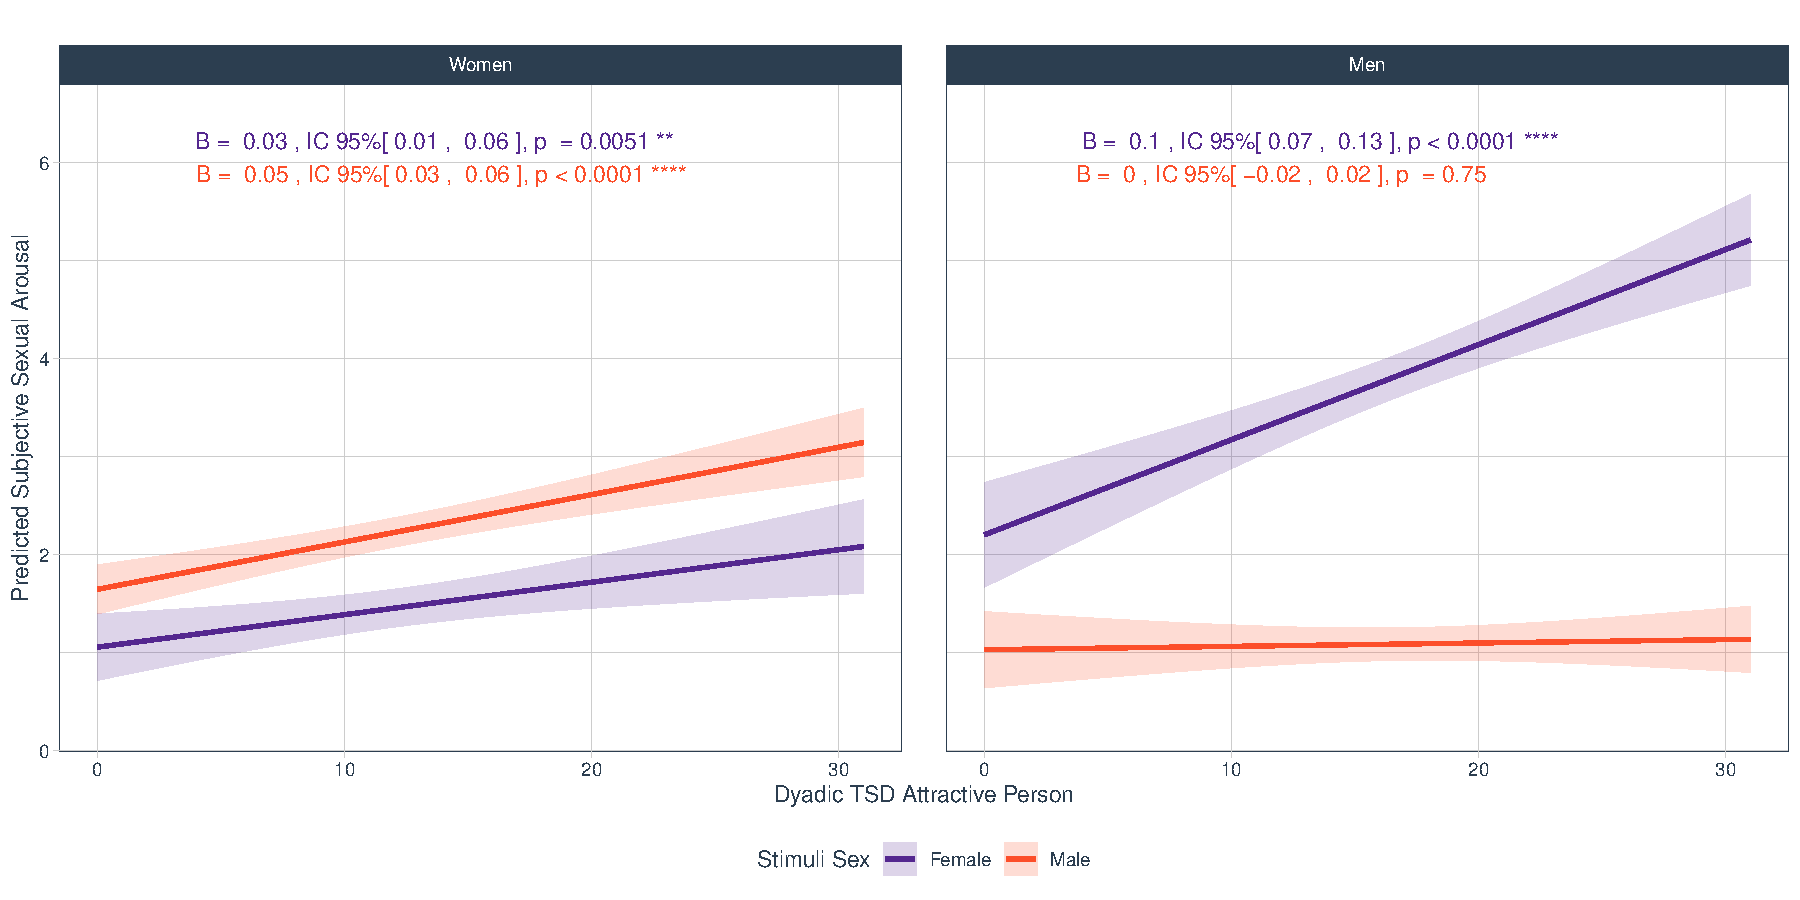
\includegraphics{Sexual_Desire_Arousal_anonymous_files/figure-latex/fig-h2b-1.pdf}
\caption{\label{fig:fig-h2b}Predicted subjective sexual arousal as a function of Dyadic TSD Partner, modeled using aLinear Mixed Model (LMM). Lines represent predicted values, and shaded areas indicate 95\% confidence intervals. The model include participant gender and stimuli sex as key factors.}
\end{figure}

\subsubsection{Hypothesis 2c: Dyadic TSD Partner}\label{hyp2c}

\paragraph{Model Robustness: Examining the Effects of Dyadic TSD Partner on SSA Across Gender and Stimuli Sex}\label{model-robustness-examining-the-effects-of-dyadic-tsd-partner-on-ssa-across-gender-and-stimuli-sex}

To assess the robustness of our findings, we fitted three different models examining how Dyadic TSD Partner predicts SSA, considering variations by gender and stimuli sex:

\begin{enumerate}
\def\labelenumi{\arabic{enumi}.}
\tightlist
\item
  Cumulative Link Mixed Model (CLMM) -- \texttt{m2c\_clmm} (for ordinal outcomes, using a probit link).
\item
  Generalized Linear Mixed Model (GLMM) with Poisson family -- \texttt{m2c\_poisson} (treating SSA as a count variable).
\item
  Linear Mixed Model (LMM) -- \texttt{m2c\_lmer} (treating SSA as a continuous variable).
\end{enumerate}

\begin{Shaded}
\begin{Highlighting}[]
\CommentTok{\# Fit three different models to examine how Dyadic TSD Partner predicts SSA}
\CommentTok{\# Each model considers variations by Gender and Stimuli Sex}

\CommentTok{\# (1) Cumulative Link Mixed Model (CLMM) {-} Ordinal outcome with probit link}
\NormalTok{m2c\_clmm }\OtherTok{\textless{}{-}} \FunctionTok{clmm}\NormalTok{(}
\NormalTok{  Subjective.sexual.arousal.factor }\SpecialCharTok{\textasciitilde{}}\NormalTok{ Dyadic.TSD.Partner }\SpecialCharTok{*}\NormalTok{ Gender }\SpecialCharTok{*}\NormalTok{ Stimuli.sex }\SpecialCharTok{+}
\NormalTok{    (}\DecValTok{1} \SpecialCharTok{|}\NormalTok{ Stimuli.code) }\SpecialCharTok{+} \CommentTok{\# Random intercept for Stimuli}
\NormalTok{    (}\DecValTok{1} \SpecialCharTok{+}\NormalTok{ Stimuli.sex }\SpecialCharTok{|}\NormalTok{ Participant), }\CommentTok{\# Random intercept \& slope for Stimuli sex}
  \AttributeTok{data =}\NormalTok{ dat\_m2,}
  \AttributeTok{link =} \StringTok{"probit"}\NormalTok{,}
  \AttributeTok{control =} \FunctionTok{list}\NormalTok{(}\AttributeTok{method =} \StringTok{"nlminb"}\NormalTok{) }\CommentTok{\# Use \textquotesingle{}nlminb\textquotesingle{} optimizer for better convergence}
\NormalTok{)}

\CommentTok{\# (2) Generalized Linear Mixed Model (GLMM) {-} Poisson regression for count data}
\NormalTok{m2c\_poisson }\OtherTok{\textless{}{-}} \FunctionTok{glmer}\NormalTok{(}
\NormalTok{  Subjective.sexual.arousal }\SpecialCharTok{\textasciitilde{}}\NormalTok{ Dyadic.TSD.Partner }\SpecialCharTok{*}\NormalTok{ Gender }\SpecialCharTok{*}\NormalTok{ Stimuli.sex }\SpecialCharTok{+}
\NormalTok{    (}\DecValTok{1} \SpecialCharTok{|}\NormalTok{ Stimuli.code) }\SpecialCharTok{+} \CommentTok{\# Random intercept for Stimuli}
\NormalTok{    (}\DecValTok{1} \SpecialCharTok{+}\NormalTok{ Stimuli.sex }\SpecialCharTok{|}\NormalTok{ Participant), }\CommentTok{\# Random intercept \& slope for Stimuli sex}
  \AttributeTok{data =}\NormalTok{ dat\_m2,}
  \AttributeTok{family =}\NormalTok{ poisson }\CommentTok{\# Poisson distribution for count data}
\NormalTok{)}

\CommentTok{\# (3) Linear Mixed Model (LMM) {-} Continuous approximation}
\NormalTok{m2c\_lmer }\OtherTok{\textless{}{-}} \FunctionTok{lmer}\NormalTok{(}
\NormalTok{  Subjective.sexual.arousal }\SpecialCharTok{\textasciitilde{}}\NormalTok{ Dyadic.TSD.Partner }\SpecialCharTok{*}\NormalTok{ Gender }\SpecialCharTok{*}\NormalTok{ Stimuli.sex }\SpecialCharTok{+}
\NormalTok{    (}\DecValTok{1} \SpecialCharTok{|}\NormalTok{ Stimuli.code) }\SpecialCharTok{+} \CommentTok{\# Random intercept for Stimuli}
\NormalTok{    (}\DecValTok{1} \SpecialCharTok{+}\NormalTok{ Stimuli.sex }\SpecialCharTok{|}\NormalTok{ Participant), }\CommentTok{\# Random intercept \& slope for Stimuli sex}
  \AttributeTok{data =}\NormalTok{ dat\_m2,}
  \AttributeTok{control =} \FunctionTok{lmerControl}\NormalTok{(}\AttributeTok{optimizer =} \StringTok{"bobyqa"}\NormalTok{) }\CommentTok{\# Use \textquotesingle{}bobyqa\textquotesingle{} optimizer for stability}
\NormalTok{)}
\end{Highlighting}
\end{Shaded}

\subparagraph{Table \ref{tab:tab-robu-m2c}. ANOVA-type table of fixed effects (main effects and interactions) across the three fitted models}\label{table-reftabtab-robu-m2c.-anova-type-table-of-fixed-effects-main-effects-and-interactions-across-the-three-fitted-models}

As shown in the table below, the pattern of significant effects remains consistent across all three models, except for the main effect of gender, which is not significant in the CLMM.

\begin{Shaded}
\begin{Highlighting}[]
\CommentTok{\# Compare ANOVA{-}type tables across the three fitted models}
\CommentTok{\# This evaluates fixed effects (main effects \& interactions) for Dyadic TSD Partner on SSA}
\FunctionTok{anova.comp}\NormalTok{(}
  \AttributeTok{CLMMmod =}\NormalTok{ m2c\_clmm, }\CommentTok{\# Cumulative Link Mixed Model}
  \AttributeTok{GLMERmod =}\NormalTok{ m2c\_poisson, }\CommentTok{\# Generalized Linear Mixed Model (Poisson)}
  \AttributeTok{LMERmod =}\NormalTok{ m2c\_lmer, }\CommentTok{\# Linear Mixed Model}
  \AttributeTok{hypothesis =} \StringTok{"2c"} \CommentTok{\# Specifies hypothesis 2c}
\NormalTok{)}
\end{Highlighting}
\end{Shaded}

\begin{table}[H]
\centering
\caption{\label{tab:tab-robu-m2c}Comparison of fixed effects across the three models for Hypothesis 2c: CLMM, GLMM (Poisson), and LMM.}
\centering
\resizebox{\ifdim\width>\linewidth\linewidth\else\width\fi}{!}{
\begin{threeparttable}
\begin{tabular}[t]{lccccccccc}
\toprule
\multicolumn{1}{c}{ } & \multicolumn{3}{c}{CLMM} & \multicolumn{3}{c}{GLMER (Poisson)} & \multicolumn{3}{c}{LMM} \\
\cmidrule(l{3pt}r{3pt}){2-4} \cmidrule(l{3pt}r{3pt}){5-7} \cmidrule(l{3pt}r{3pt}){8-10}
Effect & $df$ & $\chi^2$ & $p$ & $df$ & $\chi^2$ & $p$ & $df$ & $F$ & $p$\\
\midrule
Dyadic TSD Partner & 1 & 0.642 & 0.42 & 1 & 5.150 & \textbf{0.0232} & 1, 316 & 6.589 & \textbf{0.0107}\\
Gender & 1 & 0.743 & 0.39 & 1 & 0.078 & 0.78 & 1, 316 & 0.034 & 0.85\\
Stimuli sex & 1 & 10.881 & \textbf{< 0.001} & 1 & 2.688 & 0.1 & 1, 344.42 & 0.991 & 0.32\\
Dyadic TSD Partner × Gender & 1 & 0.310 & 0.58 & 1 & 2.111 & 0.15 & 1, 316 & 3.967 & \textbf{0.0472}\\
Dyadic TSD Partner × Stimuli sex & 1 & 2.366 & 0.12 & 1 & 5.423 & \textbf{0.0199} & 1, 316 & 8.458 & \textbf{0.0039}\\
Gender × Stimuli sex & 1 & 61.739 & \textbf{< 0.0001} & 1 & 45.783 & \textbf{< 0.0001} & 1, 316 & 20.549 & \textbf{< 0.0001}\\
Dyadic TSD Partner × Gender × Stimuli sex & 1 & 1.254 & 0.26 & 1 & 2.461 & 0.12 & 1, 316 & 5.700 & \textbf{0.0176}\\
\bottomrule
\end{tabular}
\begin{tablenotes}[para]
\item \textit{Note: } 
\item For CLMM and GLMER (Poisson) models, results are
              Analysis of Deviance (Type III Wald chi-square tests),
              while for LMM, results are from an Analysis of Variance
              (Type III ANOVA with Satterthwaite's method).
              Significant effects are in bold.
\end{tablenotes}
\end{threeparttable}}
\end{table}

\subparagraph{Figure \ref{fig:preds-m2c}: Model-based predictions for Hypothesis 2c.}\label{figure-reffigpreds-m2c-model-based-predictions-for-hypothesis-2c.}

This figure presents model-based predictions of subjective sexual arousal as a function of Dyadic TSD Partner, across different stimulus sexes and participant genders. The three subplots correspond to the three statistical models used for analysis: (a) Cumulative Link Mixed Model (CLMM), (b) Generalized Linear Mixed Model (GLMM, Poisson), and (c) Linear Mixed Model (LMM). Shaded areas represent 95\% confidence intervals.

\begin{Shaded}
\begin{Highlighting}[]
\CommentTok{\# Generate model{-}based predictions for Dyadic TSD Partner on SSA}
\CommentTok{\# across different statistical models (CLMM, GLMER, LMM)}

\CommentTok{\# CLMM Predictions}
\NormalTok{p\_m2c\_clmm }\OtherTok{\textless{}{-}} \FunctionTok{emmeans}\NormalTok{(m2c\_clmm, }\SpecialCharTok{\textasciitilde{}}\NormalTok{ Dyadic.TSD.Partner }\SpecialCharTok{|}\NormalTok{ Gender }\SpecialCharTok{*}\NormalTok{ Stimuli.sex,}
  \AttributeTok{at =} \FunctionTok{list}\NormalTok{(}\AttributeTok{Dyadic.TSD.Partner =} \FunctionTok{seq}\NormalTok{(}\DecValTok{0}\NormalTok{, }\DecValTok{31}\NormalTok{, }\AttributeTok{length.out =} \DecValTok{100}\NormalTok{)),}
  \AttributeTok{mode =} \StringTok{"mean.class"}
\NormalTok{) }\SpecialCharTok{|\textgreater{}}
  \FunctionTok{as.data.frame}\NormalTok{() }\SpecialCharTok{|\textgreater{}}
  \FunctionTok{ggplot}\NormalTok{(}\FunctionTok{aes}\NormalTok{(}
    \AttributeTok{x =}\NormalTok{ Dyadic.TSD.Partner, }\AttributeTok{y =}\NormalTok{ mean.class,}
    \AttributeTok{color =}\NormalTok{ Stimuli.sex, }\AttributeTok{fill =}\NormalTok{ Stimuli.sex}
\NormalTok{  )) }\SpecialCharTok{+}
  \FunctionTok{geom\_line}\NormalTok{(}\AttributeTok{size =} \DecValTok{1}\NormalTok{) }\SpecialCharTok{+}
  \FunctionTok{geom\_ribbon}\NormalTok{(}\FunctionTok{aes}\NormalTok{(}\AttributeTok{ymin =}\NormalTok{ asymp.LCL, }\AttributeTok{ymax =}\NormalTok{ asymp.UCL), }\AttributeTok{alpha =} \FloatTok{0.2}\NormalTok{, }\AttributeTok{color =} \ConstantTok{NA}\NormalTok{) }\SpecialCharTok{+}
  \FunctionTok{scale\_color\_manual}\NormalTok{(}\AttributeTok{values =}\NormalTok{ color.StimuliSex) }\SpecialCharTok{+}
  \FunctionTok{scale\_fill\_manual}\NormalTok{(}\AttributeTok{values =}\NormalTok{ color.StimuliSex) }\SpecialCharTok{+}
  \FunctionTok{facet\_wrap}\NormalTok{(}\SpecialCharTok{\textasciitilde{}}\NormalTok{Gender, }\AttributeTok{ncol =} \DecValTok{1}\NormalTok{) }\SpecialCharTok{+}
  \FunctionTok{labs}\NormalTok{(}
    \AttributeTok{y =} \StringTok{"Predicted Subjective Sexual Arousal"}\NormalTok{,}
    \AttributeTok{x =} \StringTok{"Dyadic TSD Partner"}\NormalTok{,}
    \AttributeTok{title =} \StringTok{"CLMM"}\NormalTok{,}
    \AttributeTok{color =} \StringTok{"Stimuli Sex"}\NormalTok{, }\AttributeTok{fill =} \StringTok{"Stimuli Sex"}
\NormalTok{  ) }\SpecialCharTok{+}
  \FunctionTok{theme\_tq}\NormalTok{() }\SpecialCharTok{+}
  \FunctionTok{theme}\NormalTok{(}\AttributeTok{legend.position =} \StringTok{"bottom"}\NormalTok{) }\SpecialCharTok{+}
  \FunctionTok{ylim}\NormalTok{(}\FunctionTok{c}\NormalTok{(}\FloatTok{0.3}\NormalTok{, }\FloatTok{5.3}\NormalTok{))}

\CommentTok{\# Poisson GLMM Predictions}
\NormalTok{p\_m2c\_poisson }\OtherTok{\textless{}{-}} \FunctionTok{emmeans}\NormalTok{(m2c\_poisson, }\SpecialCharTok{\textasciitilde{}}\NormalTok{ Dyadic.TSD.Partner }\SpecialCharTok{|}\NormalTok{ Gender }\SpecialCharTok{*}\NormalTok{ Stimuli.sex,}
  \AttributeTok{at =} \FunctionTok{list}\NormalTok{(}\AttributeTok{Dyadic.TSD.Partner =} \FunctionTok{seq}\NormalTok{(}\DecValTok{0}\NormalTok{, }\DecValTok{31}\NormalTok{, }\AttributeTok{length.out =} \DecValTok{100}\NormalTok{)),}
  \AttributeTok{type =} \StringTok{"response"}
\NormalTok{) }\SpecialCharTok{|\textgreater{}}
  \FunctionTok{as.data.frame}\NormalTok{() }\SpecialCharTok{|\textgreater{}}
  \FunctionTok{ggplot}\NormalTok{(}\FunctionTok{aes}\NormalTok{(}
    \AttributeTok{x =}\NormalTok{ Dyadic.TSD.Partner, }\AttributeTok{y =}\NormalTok{ rate,}
    \AttributeTok{color =}\NormalTok{ Stimuli.sex, }\AttributeTok{fill =}\NormalTok{ Stimuli.sex}
\NormalTok{  )) }\SpecialCharTok{+}
  \FunctionTok{geom\_line}\NormalTok{(}\AttributeTok{size =} \DecValTok{1}\NormalTok{) }\SpecialCharTok{+}
  \FunctionTok{geom\_ribbon}\NormalTok{(}\FunctionTok{aes}\NormalTok{(}\AttributeTok{ymin =}\NormalTok{ asymp.LCL, }\AttributeTok{ymax =}\NormalTok{ asymp.UCL), }\AttributeTok{alpha =} \FloatTok{0.2}\NormalTok{, }\AttributeTok{color =} \ConstantTok{NA}\NormalTok{) }\SpecialCharTok{+}
  \FunctionTok{scale\_color\_manual}\NormalTok{(}\AttributeTok{values =}\NormalTok{ color.StimuliSex) }\SpecialCharTok{+}
  \FunctionTok{scale\_fill\_manual}\NormalTok{(}\AttributeTok{values =}\NormalTok{ color.StimuliSex) }\SpecialCharTok{+}
  \FunctionTok{facet\_wrap}\NormalTok{(}\SpecialCharTok{\textasciitilde{}}\NormalTok{Gender, }\AttributeTok{ncol =} \DecValTok{1}\NormalTok{) }\SpecialCharTok{+}
  \FunctionTok{labs}\NormalTok{(}
    \AttributeTok{y =} \StringTok{""}\NormalTok{, }\AttributeTok{x =} \StringTok{"Dyadic TSD Partner"}\NormalTok{,}
    \AttributeTok{title =} \StringTok{"GLMER (Poisson)"}\NormalTok{,}
    \AttributeTok{color =} \StringTok{"Stimuli Sex"}\NormalTok{, }\AttributeTok{fill =} \StringTok{"Stimuli Sex"}
\NormalTok{  ) }\SpecialCharTok{+}
  \FunctionTok{theme\_tq}\NormalTok{() }\SpecialCharTok{+}
  \FunctionTok{theme}\NormalTok{(}\AttributeTok{legend.position =} \StringTok{"bottom"}\NormalTok{) }\SpecialCharTok{+}
  \FunctionTok{ylim}\NormalTok{(}\FunctionTok{c}\NormalTok{(}\FloatTok{0.3}\NormalTok{, }\FloatTok{5.3}\NormalTok{))}

\CommentTok{\# LMM Predictions}
\NormalTok{p\_m2c\_lmer }\OtherTok{\textless{}{-}} \FunctionTok{emmeans}\NormalTok{(m2c\_lmer, }\SpecialCharTok{\textasciitilde{}}\NormalTok{ Dyadic.TSD.Partner }\SpecialCharTok{|}\NormalTok{ Gender }\SpecialCharTok{*}\NormalTok{ Stimuli.sex,}
  \AttributeTok{at =} \FunctionTok{list}\NormalTok{(}\AttributeTok{Dyadic.TSD.Partner =} \FunctionTok{seq}\NormalTok{(}\DecValTok{0}\NormalTok{, }\DecValTok{31}\NormalTok{, }\AttributeTok{length.out =} \DecValTok{100}\NormalTok{)),}
  \AttributeTok{type =} \StringTok{"response"}
\NormalTok{) }\SpecialCharTok{|\textgreater{}}
  \FunctionTok{as.data.frame}\NormalTok{() }\SpecialCharTok{|\textgreater{}}
  \FunctionTok{ggplot}\NormalTok{(}\FunctionTok{aes}\NormalTok{(}
    \AttributeTok{x =}\NormalTok{ Dyadic.TSD.Partner, }\AttributeTok{y =}\NormalTok{ emmean,}
    \AttributeTok{color =}\NormalTok{ Stimuli.sex, }\AttributeTok{fill =}\NormalTok{ Stimuli.sex}
\NormalTok{  )) }\SpecialCharTok{+}
  \FunctionTok{geom\_line}\NormalTok{(}\AttributeTok{size =} \DecValTok{1}\NormalTok{) }\SpecialCharTok{+}
  \FunctionTok{geom\_ribbon}\NormalTok{(}\FunctionTok{aes}\NormalTok{(}\AttributeTok{ymin =}\NormalTok{ asymp.LCL, }\AttributeTok{ymax =}\NormalTok{ asymp.UCL), }\AttributeTok{alpha =} \FloatTok{0.2}\NormalTok{, }\AttributeTok{color =} \ConstantTok{NA}\NormalTok{) }\SpecialCharTok{+}
  \FunctionTok{scale\_color\_manual}\NormalTok{(}\AttributeTok{values =}\NormalTok{ color.StimuliSex) }\SpecialCharTok{+}
  \FunctionTok{scale\_fill\_manual}\NormalTok{(}\AttributeTok{values =}\NormalTok{ color.StimuliSex) }\SpecialCharTok{+}
  \FunctionTok{facet\_wrap}\NormalTok{(}\SpecialCharTok{\textasciitilde{}}\NormalTok{Gender, }\AttributeTok{ncol =} \DecValTok{1}\NormalTok{) }\SpecialCharTok{+}
  \FunctionTok{labs}\NormalTok{(}
    \AttributeTok{y =} \StringTok{""}\NormalTok{, }\AttributeTok{x =} \StringTok{"Dyadic TSD Partner"}\NormalTok{,}
    \AttributeTok{title =} \StringTok{"LMM"}\NormalTok{,}
    \AttributeTok{color =} \StringTok{"Stimuli Sex"}\NormalTok{, }\AttributeTok{fill =} \StringTok{"Stimuli Sex"}
\NormalTok{  ) }\SpecialCharTok{+}
  \FunctionTok{theme\_tq}\NormalTok{() }\SpecialCharTok{+}
  \FunctionTok{theme}\NormalTok{(}\AttributeTok{legend.position =} \StringTok{"bottom"}\NormalTok{) }\SpecialCharTok{+}
  \FunctionTok{ylim}\NormalTok{(}\FunctionTok{c}\NormalTok{(}\FloatTok{0.3}\NormalTok{, }\FloatTok{5.3}\NormalTok{))}

\CommentTok{\# Arrange plots into a single figure}
\NormalTok{p\_robu\_m2c }\OtherTok{\textless{}{-}} \FunctionTok{ggarrange}\NormalTok{(p\_m2c\_clmm, p\_m2c\_poisson, p\_m2c\_lmer,}
  \AttributeTok{common.legend =} \ConstantTok{TRUE}\NormalTok{, }\AttributeTok{labels =} \StringTok{"auto"}\NormalTok{, }\AttributeTok{legend =} \StringTok{"bottom"}\NormalTok{, }\AttributeTok{nrow =} \DecValTok{1}
\NormalTok{)}

\CommentTok{\# Display the combined figure}
\NormalTok{p\_robu\_m2c}
\end{Highlighting}
\end{Shaded}

\begin{figure}
\centering
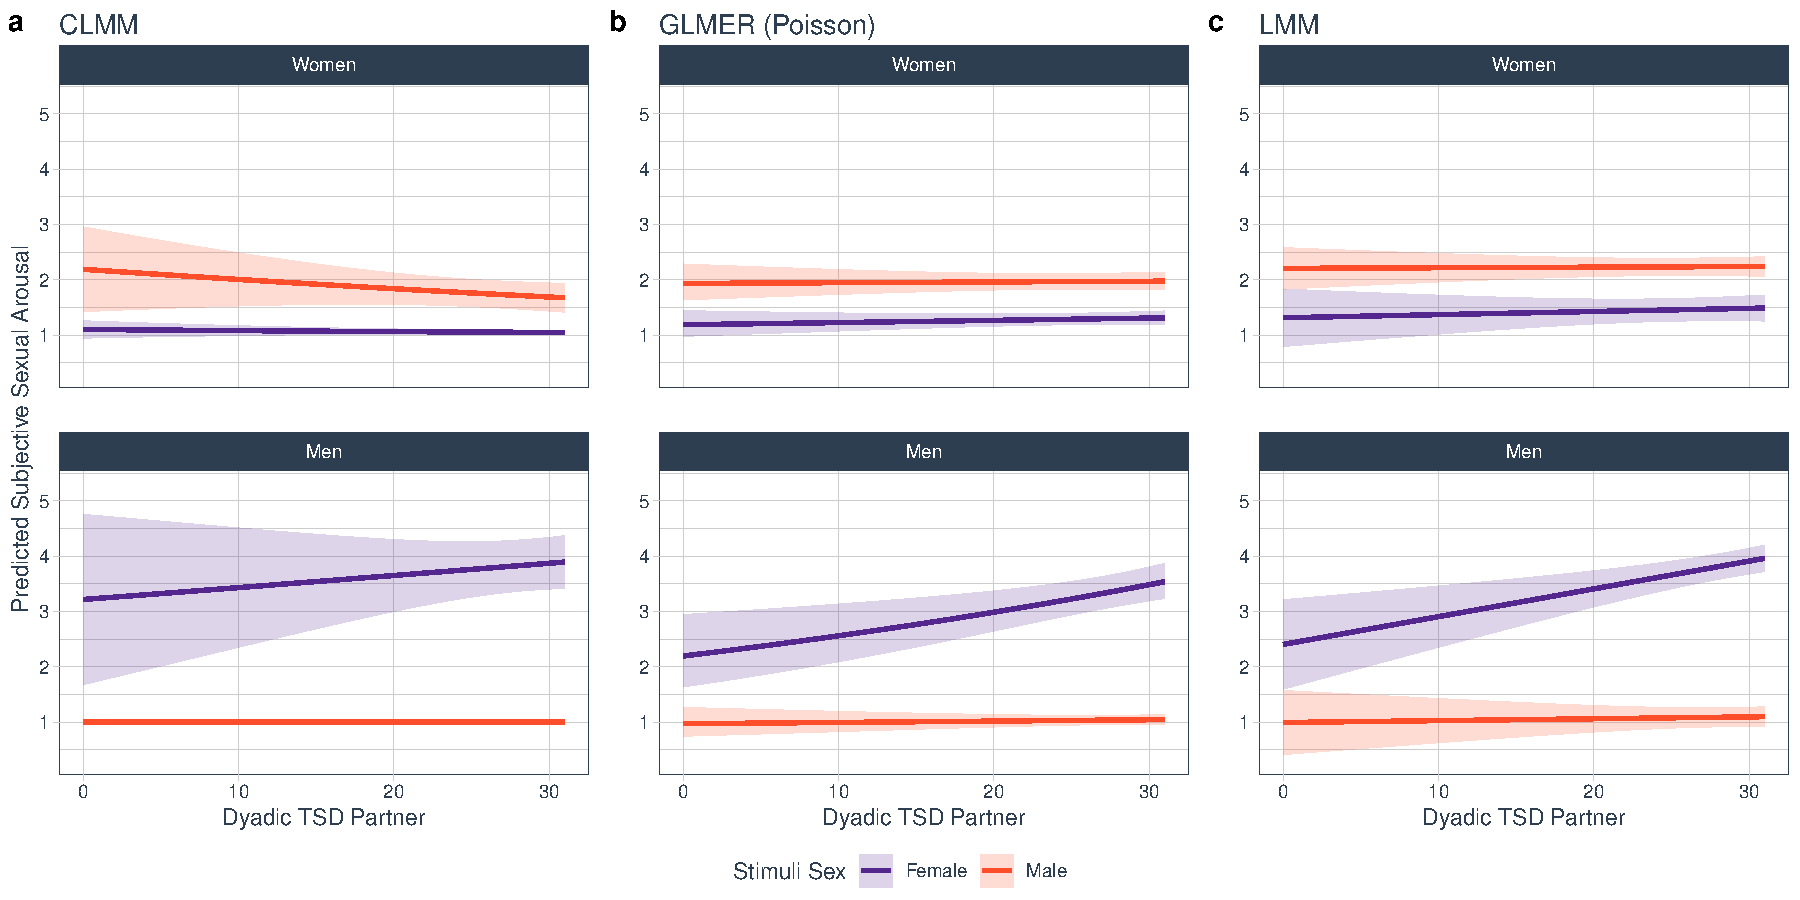
\includegraphics{Sexual_Desire_Arousal_anonymous_files/figure-latex/preds-m2c-1.pdf}
\caption{\label{fig:preds-m2c}Predicted subjective sexual arousal as a function of Dyadic TSD Partner, modeled using three statistical approaches: \textbf{(a)} Cumulative Link Mixed Model (CLMM); \textbf{(b)} Generalized Linear Mixed Model (GLMM) with a Poisson family; \textbf{(c)} Linear Mixed Model (LMM). Lines represent predicted values, and shaded areas indicate 95\% confidence intervals. The models include participant gender and stimulus sex as key factors.}
\end{figure}

\paragraph{Final Model: Effects of Dyadic TSD Partner on SSA Across Gender and Stimuli Sex}\label{final-model-effects-of-dyadic-tsd-partner-on-ssa-across-gender-and-stimuli-sex}

Given the apparent robustness of most results across models (CLMM, GLMER and LMM; Table \ref{tab:tab-robu-m2c}, Fig. \ref{fig:preds-m2c}), we test the predictions of the hypothesis from the LMM (\texttt{m2c\_lmer}).

\subparagraph{\texorpdfstring{Table \ref{tab:tab-m2c}. ANOVA-type table for the interaction between \texttt{Relationship\ type}, and \texttt{Gender}}{Table \ref{tab:tab-m2c}. ANOVA-type table for the interaction between Relationship type, and Gender}}\label{table-reftabtab-m2c.-anova-type-table-for-the-interaction-between-relationship-type-and-gender}

This tables summarizes the results of the model.

\begin{Shaded}
\begin{Highlighting}[]
\CommentTok{\# Generate ANOVA{-}type table for the final LMM model}
\CommentTok{\# This summarizes the effects of Dyadic TSD Partner on SSA across Gender and Stimuli Sex}
\FunctionTok{anova.sig.lmer}\NormalTok{(}
  \AttributeTok{model =}\NormalTok{ m2c\_lmer, }\CommentTok{\# Use LMM as the final model}
  \AttributeTok{custom\_caption =} \StringTok{"Effects of Dyadic TSD Partner on SSA Across Gender and Stimuli Sex"}
\NormalTok{)}
\end{Highlighting}
\end{Shaded}

\begin{table}[H]
\centering
\caption{\label{tab:tab-m2c}Effects of Dyadic TSD Partner on SSA Across Gender and Stimuli Sex}
\centering
\resizebox{\ifdim\width>\linewidth\linewidth\else\width\fi}{!}{
\begin{threeparttable}
\begin{tabular}[t]{lcccc}
\toprule
Effect & $df$ & $F$ & $p$ & $\epsilon^2_p$\\
\midrule
Dyadic TSD Partner & 1, 316 & 6.59 & \textbf{0.0107} & 0.0173\\
Gender & 1, 316 & 0.03 & 0.85 & < 0.0001\\
Stimuli sex & 1, 344.42 & 0.99 & 0.32 & < 0.0001\\
Dyadic TSD Partner × Gender & 1, 316 & 3.97 & \textbf{0.0472} & 0.0093\\
Dyadic TSD Partner × Stimuli sex & 1, 316 & 8.46 & \textbf{0.0039} & 0.023\\
Gender × Stimuli sex & 1, 316 & 20.55 & \textbf{< 0.0001} & 0.06\\
Dyadic TSD Partner × Gender × Stimuli sex & 1, 316 & 5.70 & \textbf{0.0176} & 0.0146\\
\bottomrule
\end{tabular}
\begin{tablenotes}[para]
\item \textit{Note: } 
\item Results are Type III ANOVA. $R^2_{conditional}$ = 0.745, $R^2_{marginal}$ = 0.329. As effect size, we report partial epsilon squared ($\epsilon^2_p$), a less biased estimate than $\eta^2$ (see \cite{albersWhenPowerAnalyses2018}). Significant effects are in bold.
\end{tablenotes}
\end{threeparttable}}
\end{table}

\subparagraph{\texorpdfstring{\emph{Post-hoc} tests}{Post-hoc tests}}\label{post-hoc-tests-2}

To test the hypothesis, which predicted that there would be different relationship between SSA and Dyadic TSD Partner, and that this association differ between men and women depending on the sex of stimuli, we used simple slope analysis.

\begin{Shaded}
\begin{Highlighting}[]
\CommentTok{\# Perform simple slopes analysis for Dyadic TSD Partner on SSA}
\NormalTok{slop.m2c\_lmer }\OtherTok{\textless{}{-}} \FunctionTok{sim\_slopes}\NormalTok{(}
\NormalTok{  m2c\_lmer,}
  \AttributeTok{pred =}\NormalTok{ Dyadic.TSD.Partner,}
  \AttributeTok{modx =}\NormalTok{ Stimuli.sex,}
  \AttributeTok{mod2 =}\NormalTok{ Gender,}
  \AttributeTok{confint =} \ConstantTok{TRUE}
\NormalTok{)}

\CommentTok{\# Combine results for both genders}
\NormalTok{slop.m2c\_lmer.tab }\OtherTok{\textless{}{-}} \FunctionTok{bind\_rows}\NormalTok{(}
\NormalTok{  slop.m2c\_lmer}\SpecialCharTok{$}\NormalTok{slopes[[}\DecValTok{1}\NormalTok{]] }\SpecialCharTok{|\textgreater{}} \FunctionTok{mutate}\NormalTok{(}\AttributeTok{Gender =} \StringTok{"Women"}\NormalTok{),}
\NormalTok{  slop.m2c\_lmer}\SpecialCharTok{$}\NormalTok{slopes[[}\DecValTok{2}\NormalTok{]] }\SpecialCharTok{|\textgreater{}} \FunctionTok{mutate}\NormalTok{(}\AttributeTok{Gender =} \StringTok{"Men"}\NormalTok{)}
\NormalTok{) }\SpecialCharTok{|\textgreater{}}
  \FunctionTok{mutate}\NormalTok{(}
    \AttributeTok{Gender =} \FunctionTok{recode\_factor}\NormalTok{(Gender, }\AttributeTok{Femenino =} \StringTok{"Women"}\NormalTok{, }\AttributeTok{Masculino =} \StringTok{"Men"}\NormalTok{)}
\NormalTok{  ) }\SpecialCharTok{|\textgreater{}}
  \FunctionTok{select}\NormalTok{(Gender, }\StringTok{\textasciigrave{}}\AttributeTok{Value of Stimuli.sex}\StringTok{\textasciigrave{}}\NormalTok{, Est., }\StringTok{\textasciigrave{}}\AttributeTok{2.5\%}\StringTok{\textasciigrave{}}\NormalTok{, }\StringTok{\textasciigrave{}}\AttributeTok{97.5\%}\StringTok{\textasciigrave{}}\NormalTok{, }\StringTok{\textasciigrave{}}\AttributeTok{t val.}\StringTok{\textasciigrave{}}\NormalTok{, p) }\SpecialCharTok{|\textgreater{}}
  \FunctionTok{mutate}\NormalTok{(}
    \FunctionTok{across}\NormalTok{(}\FunctionTok{c}\NormalTok{(Est., }\StringTok{\textasciigrave{}}\AttributeTok{2.5\%}\StringTok{\textasciigrave{}}\NormalTok{, }\StringTok{\textasciigrave{}}\AttributeTok{97.5\%}\StringTok{\textasciigrave{}}\NormalTok{, }\StringTok{\textasciigrave{}}\AttributeTok{t val.}\StringTok{\textasciigrave{}}\NormalTok{, p), as.numeric),}
    \FunctionTok{across}\NormalTok{(}\FunctionTok{c}\NormalTok{(Est., }\StringTok{\textasciigrave{}}\AttributeTok{2.5\%}\StringTok{\textasciigrave{}}\NormalTok{, }\StringTok{\textasciigrave{}}\AttributeTok{97.5\%}\StringTok{\textasciigrave{}}\NormalTok{, }\StringTok{\textasciigrave{}}\AttributeTok{t val.}\StringTok{\textasciigrave{}}\NormalTok{), round, }\DecValTok{2}\NormalTok{),}
    \AttributeTok{sig =} \FunctionTok{pval.stars}\NormalTok{(p)}
\NormalTok{  ) }\SpecialCharTok{|\textgreater{}}
  \FunctionTok{rename}\NormalTok{(}
    \StringTok{"Stimuli.sex"} \OtherTok{=} \StringTok{\textasciigrave{}}\AttributeTok{Value of Stimuli.sex}\StringTok{\textasciigrave{}}\NormalTok{,}
    \StringTok{"Coefficient"} \OtherTok{=}\NormalTok{ Est.}
\NormalTok{  )}

\CommentTok{\# Create a formatted results table}
\NormalTok{slop.m2c\_lmer.tab[, }\SpecialCharTok{{-}}\FunctionTok{c}\NormalTok{(}\DecValTok{1}\NormalTok{, }\DecValTok{8}\NormalTok{)] }\SpecialCharTok{|\textgreater{}}
  \FunctionTok{mutate}\NormalTok{(}\AttributeTok{p =} \FunctionTok{pval.lev}\NormalTok{(p)) }\SpecialCharTok{|\textgreater{}}
  \FunctionTok{kable}\NormalTok{(}
    \AttributeTok{booktabs =} \ConstantTok{TRUE}\NormalTok{,}
    \AttributeTok{align =} \FunctionTok{c}\NormalTok{(}\StringTok{"l"}\NormalTok{, }\FunctionTok{rep}\NormalTok{(}\StringTok{"c"}\NormalTok{, }\DecValTok{5}\NormalTok{)),}
    \AttributeTok{caption =} \StringTok{"Slope for Dyadic TSD Partner on Subjective sexual arousal by}
\StringTok{    stimuli sex and gender"}\NormalTok{,}
    \AttributeTok{linesep =} \StringTok{""}\NormalTok{,}
    \AttributeTok{col.names =} \FunctionTok{c}\NormalTok{(}
      \StringTok{"Stimuli sex"}\NormalTok{, }\StringTok{"$B$"}\NormalTok{, }\StringTok{"$2.5}\SpecialCharTok{\textbackslash{}\textbackslash{}}\StringTok{\% CI$"}\NormalTok{, }\StringTok{"$97.5}\SpecialCharTok{\textbackslash{}\textbackslash{}}\StringTok{\% CI$"}\NormalTok{, }\StringTok{"$t$"}\NormalTok{, }\StringTok{"$p$"}
\NormalTok{    ),}
    \AttributeTok{escape =} \ConstantTok{FALSE}
\NormalTok{  ) }\SpecialCharTok{|\textgreater{}}
  \FunctionTok{kable\_styling}\NormalTok{(}\AttributeTok{latex\_options =} \FunctionTok{c}\NormalTok{(}\StringTok{"HOLD\_position"}\NormalTok{)) }\SpecialCharTok{|\textgreater{}}
  \FunctionTok{pack\_rows}\NormalTok{(}
    \AttributeTok{group\_label =} \StringTok{"Gender: Women"}\NormalTok{,}
    \AttributeTok{start\_row =} \DecValTok{1}\NormalTok{, }\AttributeTok{end\_row =} \DecValTok{2}\NormalTok{,}
    \AttributeTok{bold =} \ConstantTok{FALSE}\NormalTok{, }\AttributeTok{background =} \StringTok{"lightgray"}
\NormalTok{  ) }\SpecialCharTok{|\textgreater{}}
  \FunctionTok{pack\_rows}\NormalTok{(}
    \AttributeTok{group\_label =} \StringTok{"Gender: Men"}\NormalTok{,}
    \AttributeTok{start\_row =} \DecValTok{3}\NormalTok{, }\AttributeTok{end\_row =} \DecValTok{4}\NormalTok{,}
    \AttributeTok{bold =} \ConstantTok{FALSE}\NormalTok{, }\AttributeTok{background =} \StringTok{"lightgray"}
\NormalTok{  ) }\SpecialCharTok{|\textgreater{}}
  \FunctionTok{footnote}\NormalTok{(}
    \AttributeTok{general =} \StringTok{"$B$ represents unstandardized coefficients. No intercept is reported as}
\StringTok{    continuous predictors were centered and are dependent on this specific sample."}\NormalTok{,}
    \AttributeTok{threeparttable =} \ConstantTok{TRUE}\NormalTok{,}
    \AttributeTok{footnote\_as\_chunk =} \ConstantTok{TRUE}\NormalTok{,}
    \AttributeTok{escape =} \ConstantTok{FALSE}
\NormalTok{  )}
\end{Highlighting}
\end{Shaded}

\begin{table}[H]
\centering
\caption{\label{tab:unnamed-chunk-25}Slope for Dyadic TSD Partner on Subjective sexual arousal by
    stimuli sex and gender}
\centering
\begin{threeparttable}
\begin{tabular}[t]{lccccc}
\toprule
Stimuli sex & $B$ & $2.5\% CI$ & $97.5\% CI$ & $t$ & $p$\\
\midrule
\addlinespace[0.3em]
\multicolumn{6}{l}{\cellcolor{lightgray}{Gender: Women}}\\
\hspace{1em}Female & 0.01 & -0.01 & 0.02 & 0.58 & 0.56\\
\hspace{1em}Male & 0.00 & -0.01 & 0.01 & 0.15 & 0.88\\
\addlinespace[0.3em]
\multicolumn{6}{l}{\cellcolor{lightgray}{Gender: Men}}\\
\hspace{1em}Female & 0.05 & 0.02 & 0.08 & 3.63 & \textbf{< 0.001}\\
\hspace{1em}Male & 0.00 & -0.02 & 0.02 & 0.34 & 0.73\\
\bottomrule
\end{tabular}
\begin{tablenotes}[para]
\item \textit{Note: } 
\item $B$ represents unstandardized coefficients. No intercept is reported as
    continuous predictors were centered and are dependent on this specific sample.
\end{tablenotes}
\end{threeparttable}
\end{table}

\paragraph{Figure \ref{fig:fig-h2c}. Subjective sexual arousal to erotic stimuli: Main effects and interactions}\label{figure-reffigfig-h2c.-subjective-sexual-arousal-to-erotic-stimuli-main-effects-and-interactions}

This figure summarizes the results of hypothesis 2c.

\begin{Shaded}
\begin{Highlighting}[]
\CommentTok{\# Create the final plot for Dyadic TSD Partner on SSA}
\NormalTok{p\_m2c.fin }\OtherTok{\textless{}{-}}\NormalTok{ p\_m2c\_lmer }\SpecialCharTok{+}
  \FunctionTok{labs}\NormalTok{(}
    \AttributeTok{title =} \StringTok{""}\NormalTok{,}
    \AttributeTok{y =} \StringTok{"Predicted Subjective Sexual Arousal"}
\NormalTok{  ) }\SpecialCharTok{+}
  \FunctionTok{facet\_wrap}\NormalTok{(}\SpecialCharTok{\textasciitilde{}}\NormalTok{Gender, }\AttributeTok{ncol =} \DecValTok{2}\NormalTok{) }\SpecialCharTok{+} \CommentTok{\# Create separate facets by gender}
  \CommentTok{\# Add text labels for regression slopes}
  \FunctionTok{geom\_text}\NormalTok{(}
    \AttributeTok{data =}\NormalTok{ slop.m2c\_lmer.tab }\SpecialCharTok{|\textgreater{}} \FunctionTok{mutate}\NormalTok{(}\AttributeTok{Dyadic.TSD.Partner =} \DecValTok{2}\NormalTok{),}
    \AttributeTok{mapping =} \FunctionTok{aes}\NormalTok{(}
      \AttributeTok{x =} \FunctionTok{min}\NormalTok{(Dyadic.TSD.Partner), }\AttributeTok{y =} \ConstantTok{Inf}\NormalTok{,}
      \AttributeTok{label =} \FunctionTok{paste}\NormalTok{(}
        \StringTok{"B = "}\NormalTok{, Coefficient,}
        \StringTok{", 95\% CI ["}\NormalTok{, }\StringTok{\textasciigrave{}}\AttributeTok{2.5\%}\StringTok{\textasciigrave{}}\NormalTok{, }\StringTok{", "}\NormalTok{, }\StringTok{\textasciigrave{}}\AttributeTok{97.5\%}\StringTok{\textasciigrave{}}\NormalTok{,}
        \StringTok{"], p"}\NormalTok{, }\FunctionTok{ifelse}\NormalTok{(}\FunctionTok{grepl}\NormalTok{(}\StringTok{"\textless{}"}\NormalTok{, }\FunctionTok{pe2.lev}\NormalTok{(p)), }\FunctionTok{pe2.lev}\NormalTok{(p), }\FunctionTok{paste0}\NormalTok{(}\StringTok{" = "}\NormalTok{, }\FunctionTok{pe2.lev}\NormalTok{(p))),}
        \FunctionTok{ifelse}\NormalTok{(}\FunctionTok{is.na}\NormalTok{(sig), }\StringTok{""}\NormalTok{, sig)}
\NormalTok{      ),}
      \AttributeTok{vjust =} \DecValTok{2} \SpecialCharTok{+} \FunctionTok{as.numeric}\NormalTok{(}\FunctionTok{as.factor}\NormalTok{(Stimuli.sex)) }\SpecialCharTok{*} \DecValTok{2} \CommentTok{\# Stacks labels properly}
\NormalTok{    ),}
    \AttributeTok{hjust =} \SpecialCharTok{{-}}\FloatTok{0.1}\NormalTok{, }\CommentTok{\# Align text to the left}
    \AttributeTok{show.legend =} \ConstantTok{FALSE}
\NormalTok{  ) }\SpecialCharTok{+}
  \FunctionTok{theme}\NormalTok{(}\AttributeTok{legend.position =} \StringTok{"bottom"}\NormalTok{) }\CommentTok{\# Position legend at the bottom}

\CommentTok{\# Display the final figure}
\NormalTok{p\_m2c.fin}
\end{Highlighting}
\end{Shaded}

\begin{figure}
\centering
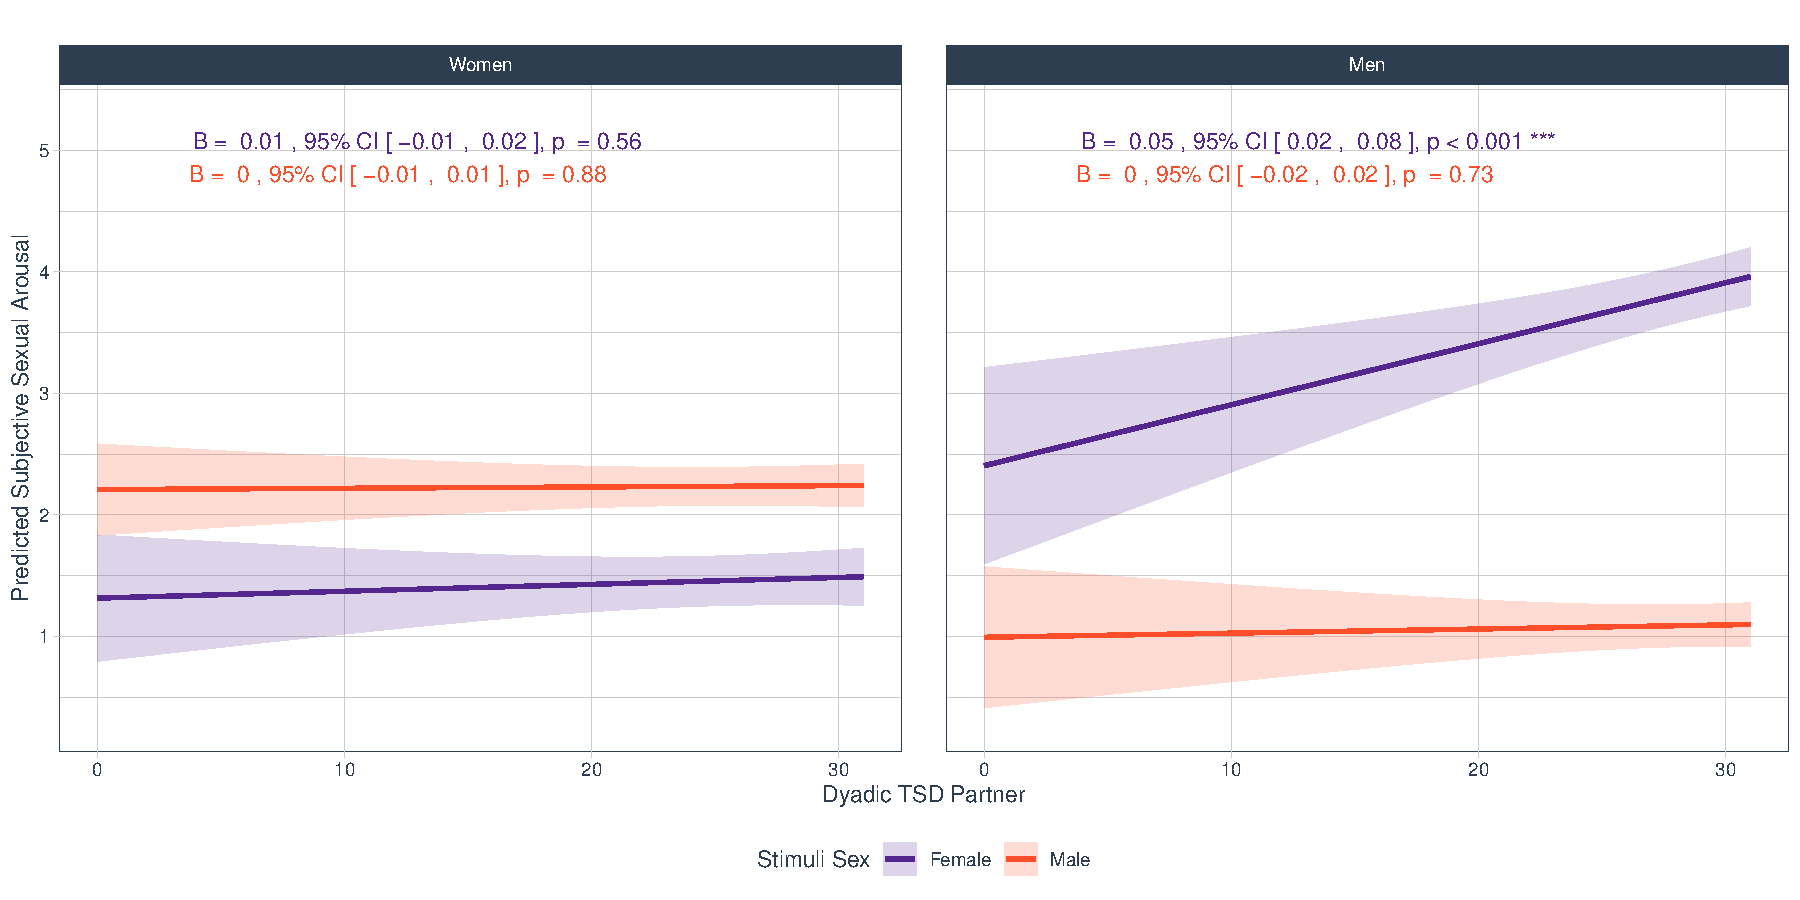
\includegraphics{Sexual_Desire_Arousal_anonymous_files/figure-latex/fig-h2c-1.pdf}
\caption{\label{fig:fig-h2c}Predicted subjective sexual arousal as a function of Dyadic TSD Partner, modeled using aLinear Mixed Model (LMM). Lines represent predicted values, and shaded areas indicate 95\% confidence intervals. The model include participant gender and stimuli sex as key factors.}
\end{figure}

\subsection{Hypothesis 3: The associations between TSD dimensions and SSA toward stimuli of self-reported preferred gender will be moderated by gender and relationship status.}\label{hyp3}

We tested whether the relationship between SSA and TSD varies across the three dimensions of TSD and whether these associations differ between men and women depending on whether they were single or not, but only in responses toward stimuli of the preferred sex. This is a fully exploratory hypothesis, for which no directional predictions were made, beyond an interaction between the TSD dimension, gender, and relationship status. As with the case of Hypothesys 2 (section \ref{hyp2}), fitted separate models for each TSD dimension:

\begin{itemize}
\tightlist
\item
  \textbf{H3a}: Solitary TSD and SSA
\item
  \textbf{H3b}: Dyadic TSD toward an attractive person
\item
  \textbf{H3c}: Dyadic TSD toward a partner
\end{itemize}

To examine this hypothesis, we modeled the effects of each of the three TSD dimension scores, gender, relationship status, and their interactions, on SSA towars stimuli of the self-reported preferred sex. We included random intercepts for each stimulus, as well as random intercepts for each participant.

\subsubsection{Modeling Approach}\label{modeling-approach-1}

Following the strategy employed for Hypothesys 2 (section \ref{hyp2}), and given that SSA is an ordinal variable with seven ordered levels, we fitted diferent models using three different approaches to ensure the robustness of our results:

\begin{enumerate}
\def\labelenumi{\arabic{enumi}.}
\tightlist
\item
  Cumulative Link Mixed Model (CLMM), using the \texttt{clmm} function from the package \texttt{ordinal} \autocite{ordinalcit}
\item
  Generalized Mixed Model (GLMM) with a Poisson family, using the \texttt{glmer} function from the package \texttt{lme4} \autocite{lme4cit}
\item
  Linear mixed model (LMM), using the \texttt{lmer} function from the package \texttt{lmerTest} \autocite{lmertestcit}
\end{enumerate}

The results across these models were largely consistent, indicating robustness in our findings. For clarity and interpretability, we primarily base our inferences on the LMM, as it provides the most straightforward interpretation and has a wider range of available functions in R for extracting model information.

\subsubsection{Data}\label{data-2}

We created a new dataset by selecting, once again, only responses to erotic stimuli but this time also filtering only responses to stimuli of the peferred sex. We also renamed key variables to remove spaces for compatibility with certain functions, and created a factor version of Subjective sexual arousal for use in the CLMM model.

\begin{Shaded}
\begin{Highlighting}[]
\CommentTok{\# Filter dataset to include only responses to erotic stimuli}
\NormalTok{dat\_m3 }\OtherTok{\textless{}{-}}\NormalTok{ dat }\SpecialCharTok{|\textgreater{}}
  \FunctionTok{filter}\NormalTok{(}\StringTok{\textasciigrave{}}\AttributeTok{Stimuli content}\StringTok{\textasciigrave{}} \SpecialCharTok{==} \StringTok{"Erotic"} \SpecialCharTok{\&}
    \StringTok{\textasciigrave{}}\AttributeTok{Stimuli sex}\StringTok{\textasciigrave{}} \SpecialCharTok{==} \StringTok{\textasciigrave{}}\AttributeTok{Preferred sex}\StringTok{\textasciigrave{}}\NormalTok{) }\SpecialCharTok{|\textgreater{}}
  \FunctionTok{rename}\NormalTok{(}
    \AttributeTok{Subjective.sexual.arousal =} \StringTok{\textasciigrave{}}\AttributeTok{Subjective sexual arousal}\StringTok{\textasciigrave{}}\NormalTok{,}
    \AttributeTok{Solitary.TSD =} \StringTok{\textasciigrave{}}\AttributeTok{Solitary sexual desire}\StringTok{\textasciigrave{}}\NormalTok{,}
    \AttributeTok{Dyadic.TSD.Attractive.Person =} \StringTok{\textasciigrave{}}\AttributeTok{Dyadic sexual desire (Attractive person)}\StringTok{\textasciigrave{}}\NormalTok{,}
    \AttributeTok{Dyadic.TSD.Partner =} \StringTok{\textasciigrave{}}\AttributeTok{Dyadic sexual desire (Partner)}\StringTok{\textasciigrave{}}\NormalTok{,}
    \AttributeTok{Stimuli.code =} \StringTok{\textasciigrave{}}\AttributeTok{Stimuli code}\StringTok{\textasciigrave{}}
\NormalTok{  ) }\SpecialCharTok{|\textgreater{}}
  \FunctionTok{mutate}\NormalTok{(}\AttributeTok{Subjective.sexual.arousal.factor =} \FunctionTok{as.factor}\NormalTok{(Subjective.sexual.arousal))}
\end{Highlighting}
\end{Shaded}

\subsubsection{Hypothesis 3a: Solitary TSD}\label{hyp3a}

\paragraph{Model Robustness: Examining the Effects of Solitary TSD on SSA Across Gender and Stimuli Sex}\label{model-robustness-examining-the-effects-of-solitary-tsd-on-ssa-across-gender-and-stimuli-sex-1}

To assess the robustness of our findings, we fitted three different models examining how Solitary TSD predicts SSA, considering variations by gender and stimuli sex:

\begin{enumerate}
\def\labelenumi{\arabic{enumi}.}
\tightlist
\item
  Cumulative Link Mixed Model (CLMM) -- \texttt{m3a\_clmm} (for ordinal outcomes, using a probit link).
\item
  Generalized Linear Mixed Model (GLMM) with Poisson family -- \texttt{m3a\_poisson} (treating SSA as a count variable).
\item
  Linear Mixed Model (LMM) -- \texttt{m3a\_lmer} (treating SSA as a continuous variable).
\end{enumerate}

\begin{Shaded}
\begin{Highlighting}[]
\CommentTok{\# (1) Cumulative Link Mixed Model (CLMM) {-} Ordinal model with probit link}
\NormalTok{m3a\_clmm }\OtherTok{\textless{}{-}} \FunctionTok{clmm}\NormalTok{(}
\NormalTok{  Subjective.sexual.arousal.factor }\SpecialCharTok{\textasciitilde{}}\NormalTok{ Solitary.TSD }\SpecialCharTok{*}\NormalTok{ Gender }\SpecialCharTok{*}\NormalTok{ Relationship }\SpecialCharTok{+}
\NormalTok{    (}\DecValTok{1} \SpecialCharTok{|}\NormalTok{ Stimuli.code) }\SpecialCharTok{+} \CommentTok{\# Random intercept for Stimuli}
\NormalTok{    (}\DecValTok{1} \SpecialCharTok{|}\NormalTok{ Participant), }\CommentTok{\# Random intercept \& slope for Relationship status}
  \AttributeTok{data =}\NormalTok{ dat\_m3,}
  \AttributeTok{link =} \StringTok{"probit"}\NormalTok{,}
  \AttributeTok{control =} \FunctionTok{list}\NormalTok{(}\AttributeTok{method =} \StringTok{"nlminb"}\NormalTok{) }\CommentTok{\# Use \textquotesingle{}nlminb\textquotesingle{} optimizer for better convergence}
\NormalTok{)}

\CommentTok{\# (2) Generalized Linear Mixed Model (GLMM) {-} Poisson regression for count data}
\NormalTok{m3a\_poisson }\OtherTok{\textless{}{-}} \FunctionTok{glmer}\NormalTok{(}
\NormalTok{  Subjective.sexual.arousal }\SpecialCharTok{\textasciitilde{}}\NormalTok{ Solitary.TSD }\SpecialCharTok{*}\NormalTok{ Gender }\SpecialCharTok{*}\NormalTok{ Relationship }\SpecialCharTok{+}
\NormalTok{    (}\DecValTok{1} \SpecialCharTok{|}\NormalTok{ Stimuli.code) }\SpecialCharTok{+} \CommentTok{\# Random intercept for Stimuli}
\NormalTok{    (}\DecValTok{1} \SpecialCharTok{|}\NormalTok{ Participant), }\CommentTok{\# Random intercept \& slope for Relationship status}
  \AttributeTok{data =}\NormalTok{ dat\_m3,}
  \AttributeTok{family =}\NormalTok{ poisson }\CommentTok{\# Poisson distribution for count data}
\NormalTok{)}

\CommentTok{\# (3) Linear Mixed Model (LMM) {-} Continuous approximation}
\NormalTok{m3a\_lmer }\OtherTok{\textless{}{-}} \FunctionTok{lmer}\NormalTok{(}
\NormalTok{  Subjective.sexual.arousal }\SpecialCharTok{\textasciitilde{}}\NormalTok{ Solitary.TSD }\SpecialCharTok{*}\NormalTok{ Gender }\SpecialCharTok{*}\NormalTok{ Relationship }\SpecialCharTok{+}
\NormalTok{    (}\DecValTok{1} \SpecialCharTok{|}\NormalTok{ Stimuli.code) }\SpecialCharTok{+} \CommentTok{\# Random intercept for Stimuli}
\NormalTok{    (}\DecValTok{1} \SpecialCharTok{|}\NormalTok{ Participant), }\CommentTok{\# Random intercept \& slope for Relationship status}
  \AttributeTok{data =}\NormalTok{ dat\_m3,}
  \AttributeTok{control =} \FunctionTok{lmerControl}\NormalTok{(}\AttributeTok{optimizer =} \StringTok{"bobyqa"}\NormalTok{) }\CommentTok{\# Use \textquotesingle{}bobyqa\textquotesingle{} optimizer for stability}
\NormalTok{)}
\end{Highlighting}
\end{Shaded}

\subparagraph{Table \ref{tab:tab-robu-m3a}. ANOVA-type table of fixed effects (main effects and interactions) across the three fitted models}\label{table-reftabtab-robu-m3a.-anova-type-table-of-fixed-effects-main-effects-and-interactions-across-the-three-fitted-models}

As shown in the table below, the pattern of significant effects remains consistent across all three models, except for the main effect of gender, which is not significant in the CLMM.

\begin{Shaded}
\begin{Highlighting}[]
\CommentTok{\# Compare fixed effects across the three models (CLMM, GLMM, LMM)}
\FunctionTok{anova.comp}\NormalTok{(}
  \AttributeTok{CLMMmod =}\NormalTok{ m3a\_clmm, }\CommentTok{\# Cumulative Link Mixed Model (ordinal outcome)}
  \AttributeTok{GLMERmod =}\NormalTok{ m3a\_poisson, }\CommentTok{\# Generalized Linear Mixed Model (Poisson family)}
  \AttributeTok{LMERmod =}\NormalTok{ m3a\_lmer, }\CommentTok{\# Linear Mixed Model (continuous outcome)}
  \AttributeTok{hypothesis =} \StringTok{"3a"} \CommentTok{\# Specifies hypothesis 3a for tracking}
\NormalTok{)}
\end{Highlighting}
\end{Shaded}

\begin{table}[H]
\centering
\caption{\label{tab:tab-robu-m3a}Comparison of fixed effects across the three models for Hypothesis 3a: CLMM, GLMM (Poisson), and LMM.}
\centering
\resizebox{\ifdim\width>\linewidth\linewidth\else\width\fi}{!}{
\begin{threeparttable}
\begin{tabular}[t]{lccccccccc}
\toprule
\multicolumn{1}{c}{ } & \multicolumn{3}{c}{CLMM} & \multicolumn{3}{c}{GLMER (Poisson)} & \multicolumn{3}{c}{LMM} \\
\cmidrule(l{3pt}r{3pt}){2-4} \cmidrule(l{3pt}r{3pt}){5-7} \cmidrule(l{3pt}r{3pt}){8-10}
Effect & $df$ & $\chi^2$ & $p$ & $df$ & $\chi^2$ & $p$ & $df$ & $F$ & $p$\\
\midrule
Solitary TSD & 1 & 10.107 & \textbf{0.0015} & 1 & 9.473 & \textbf{0.0021} & 1, 315 & 6.881 & \textbf{0.0091}\\
Gender & 1 & 16.166 & \textbf{< 0.0001} & 1 & 17.941 & \textbf{< 0.0001} & 1, 355.34 & 14.100 & \textbf{< 0.001}\\
Relationship & 1 & 0.002 & 0.97 & 1 & 0.018 & 0.89 & 1, 314.95 & 0.337 & 0.56\\
Solitary TSD × Gender & 1 & 1.632 & 0.2 & 1 & 1.291 & 0.26 & 1, 315.23 & 0.071 & 0.79\\
Solitary TSD × Relationship & 1 & 0.070 & 0.79 & 1 & 0.180 & 0.67 & 1, 314.95 & 0.531 & 0.47\\
Gender × Relationship & 1 & 3.001 & 0.08 & 1 & 2.152 & 0.14 & 1, 314.95 & 2.953 & 0.09\\
Solitary TSD × Gender × Relationship & 1 & 2.262 & 0.13 & 1 & 1.443 & 0.23 & 1, 315.08 & 2.023 & 0.16\\
\bottomrule
\end{tabular}
\begin{tablenotes}[para]
\item \textit{Note: } 
\item For CLMM and GLMER (Poisson) models, results are
              Analysis of Deviance (Type III Wald chi-square tests),
              while for LMM, results are from an Analysis of Variance
              (Type III ANOVA with Satterthwaite's method).
              Significant effects are in bold.
\end{tablenotes}
\end{threeparttable}}
\end{table}

\subparagraph{Figure \ref{fig:preds-m3a}: Model-based predictions for Hypothesis 3a.}\label{figure-reffigpreds-m3a-model-based-predictions-for-hypothesis-3a.}

This figure presents model-based predictions of subjective sexual arousal as a function of Solitary TSD, across different relationship status and participant genders. The three subplots correspond to the three statistical models used for analysis: (a) Cumulative Link Mixed Model (CLMM), (b) Generalized Linear Mixed Model (GLMM, Poisson), and (c) Linear Mixed Model (LMM). Shaded areas represent 95\% confidence intervals.

\begin{Shaded}
\begin{Highlighting}[]
\CommentTok{\# CLMM Predictions: Estimated marginal means for Solitary TSD across gender \& relationship}
\NormalTok{p\_m3a\_clmm }\OtherTok{\textless{}{-}} \FunctionTok{emmeans}\NormalTok{(m3a\_clmm, }\SpecialCharTok{\textasciitilde{}}\NormalTok{ Solitary.TSD }\SpecialCharTok{|}\NormalTok{ Gender }\SpecialCharTok{*}\NormalTok{ Relationship,}
  \AttributeTok{at =} \FunctionTok{list}\NormalTok{(}\AttributeTok{Solitary.TSD =} \FunctionTok{seq}\NormalTok{(}\DecValTok{0}\NormalTok{, }\DecValTok{31}\NormalTok{, }\AttributeTok{length.out =} \DecValTok{100}\NormalTok{)), }\CommentTok{\# Generate values for smooth curve}
  \AttributeTok{mode =} \StringTok{"mean.class"} \CommentTok{\# Predict mean response category}
\NormalTok{) }\SpecialCharTok{|\textgreater{}}
  \FunctionTok{as.data.frame}\NormalTok{() }\SpecialCharTok{|\textgreater{}} \CommentTok{\# Convert results into a dataframe for plotting}
  \FunctionTok{ggplot}\NormalTok{(}\FunctionTok{aes}\NormalTok{(}\AttributeTok{x =}\NormalTok{ Solitary.TSD, }\AttributeTok{y =}\NormalTok{ mean.class, }\AttributeTok{color =}\NormalTok{ Relationship, }\AttributeTok{fill =}\NormalTok{ Relationship)) }\SpecialCharTok{+}
  \FunctionTok{geom\_line}\NormalTok{(}\AttributeTok{size =} \DecValTok{1}\NormalTok{) }\SpecialCharTok{+} \CommentTok{\# Plot predicted means as lines}
  \FunctionTok{geom\_ribbon}\NormalTok{(}\FunctionTok{aes}\NormalTok{(}\AttributeTok{ymin =}\NormalTok{ asymp.LCL, }\AttributeTok{ymax =}\NormalTok{ asymp.UCL, }\AttributeTok{fill =}\NormalTok{ Relationship),}
    \AttributeTok{alpha =} \FloatTok{0.2}\NormalTok{, }\AttributeTok{color =} \ConstantTok{NA} \CommentTok{\# Add confidence interval as shaded ribbon}
\NormalTok{  ) }\SpecialCharTok{+}
  \FunctionTok{scale\_color\_manual}\NormalTok{(}\AttributeTok{values =}\NormalTok{ color.Relationship) }\SpecialCharTok{+} \CommentTok{\# Use predefined colors}
  \FunctionTok{scale\_fill\_manual}\NormalTok{(}\AttributeTok{values =}\NormalTok{ color.Relationship) }\SpecialCharTok{+}
  \FunctionTok{facet\_wrap}\NormalTok{(}\SpecialCharTok{\textasciitilde{}}\NormalTok{Gender, }\AttributeTok{ncol =} \DecValTok{1}\NormalTok{) }\SpecialCharTok{+} \CommentTok{\# Create separate plots for each gender}
  \FunctionTok{labs}\NormalTok{(}\AttributeTok{y =} \StringTok{"Predicted Subjective Sexual Arousal"}\NormalTok{, }\AttributeTok{x =} \StringTok{"Solitary TSD"}\NormalTok{, }
       \AttributeTok{title =} \StringTok{"CLMM"}\NormalTok{) }\SpecialCharTok{+}
  \FunctionTok{theme\_tq}\NormalTok{() }\SpecialCharTok{+} \CommentTok{\# Apply custom theme}
  \FunctionTok{theme}\NormalTok{(}\AttributeTok{legend.position =} \StringTok{"bottom"}\NormalTok{) }\SpecialCharTok{+}
  \FunctionTok{ylim}\NormalTok{(}\FunctionTok{c}\NormalTok{(}\FloatTok{0.3}\NormalTok{, }\DecValTok{6}\NormalTok{)) }\CommentTok{\# Set Y{-}axis limits}

\CommentTok{\# Poisson GLMM Predictions: Similar setup but with a Poisson distribution}
\NormalTok{p\_m3a\_poisson }\OtherTok{\textless{}{-}} \FunctionTok{emmeans}\NormalTok{(m3a\_poisson, }\SpecialCharTok{\textasciitilde{}}\NormalTok{ Solitary.TSD }\SpecialCharTok{|}\NormalTok{ Gender }\SpecialCharTok{*}\NormalTok{ Relationship,}
  \AttributeTok{at =} \FunctionTok{list}\NormalTok{(}\AttributeTok{Solitary.TSD =} \FunctionTok{seq}\NormalTok{(}\DecValTok{0}\NormalTok{, }\DecValTok{31}\NormalTok{, }\AttributeTok{length.out =} \DecValTok{100}\NormalTok{)), }\AttributeTok{type =} \StringTok{"response"}
\NormalTok{) }\SpecialCharTok{|\textgreater{}}
  \FunctionTok{as.data.frame}\NormalTok{() }\SpecialCharTok{|\textgreater{}}
  \FunctionTok{ggplot}\NormalTok{(}\FunctionTok{aes}\NormalTok{(}\AttributeTok{x =}\NormalTok{ Solitary.TSD, }\AttributeTok{y =}\NormalTok{ rate, }\AttributeTok{color =}\NormalTok{ Relationship, }\AttributeTok{fill =}\NormalTok{ Relationship)) }\SpecialCharTok{+}
  \FunctionTok{geom\_line}\NormalTok{(}\AttributeTok{size =} \DecValTok{1}\NormalTok{) }\SpecialCharTok{+}
  \FunctionTok{geom\_ribbon}\NormalTok{(}\FunctionTok{aes}\NormalTok{(}\AttributeTok{ymin =}\NormalTok{ asymp.LCL, }\AttributeTok{ymax =}\NormalTok{ asymp.UCL, }\AttributeTok{fill =}\NormalTok{ Relationship),}
    \AttributeTok{alpha =} \FloatTok{0.2}\NormalTok{, }\AttributeTok{color =} \ConstantTok{NA}
\NormalTok{  ) }\SpecialCharTok{+}
  \FunctionTok{scale\_color\_manual}\NormalTok{(}\AttributeTok{values =}\NormalTok{ color.Relationship) }\SpecialCharTok{+}
  \FunctionTok{scale\_fill\_manual}\NormalTok{(}\AttributeTok{values =}\NormalTok{ color.Relationship) }\SpecialCharTok{+}
  \FunctionTok{facet\_wrap}\NormalTok{(}\SpecialCharTok{\textasciitilde{}}\NormalTok{Gender, }\AttributeTok{ncol =} \DecValTok{1}\NormalTok{) }\SpecialCharTok{+}
  \FunctionTok{labs}\NormalTok{(}\AttributeTok{y =} \StringTok{""}\NormalTok{, }\AttributeTok{x =} \StringTok{"Solitary TSD"}\NormalTok{, }\AttributeTok{title =} \StringTok{"GLMER (Poisson)"}\NormalTok{) }\SpecialCharTok{+}
  \FunctionTok{theme\_tq}\NormalTok{() }\SpecialCharTok{+}
  \FunctionTok{theme}\NormalTok{(}\AttributeTok{legend.position =} \StringTok{"bottom"}\NormalTok{) }\SpecialCharTok{+}
  \FunctionTok{ylim}\NormalTok{(}\FunctionTok{c}\NormalTok{(}\FloatTok{0.3}\NormalTok{, }\DecValTok{6}\NormalTok{))}

\CommentTok{\# LMM Predictions: Continuous outcome using LMM}
\NormalTok{p\_m3a\_lmer }\OtherTok{\textless{}{-}} \FunctionTok{emmeans}\NormalTok{(m3a\_lmer, }\SpecialCharTok{\textasciitilde{}}\NormalTok{ Solitary.TSD }\SpecialCharTok{|}\NormalTok{ Gender }\SpecialCharTok{*}\NormalTok{ Relationship,}
  \AttributeTok{at =} \FunctionTok{list}\NormalTok{(}\AttributeTok{Solitary.TSD =} \FunctionTok{seq}\NormalTok{(}\DecValTok{0}\NormalTok{, }\DecValTok{31}\NormalTok{, }\AttributeTok{length.out =} \DecValTok{100}\NormalTok{)), }\AttributeTok{type =} \StringTok{"response"}
\NormalTok{) }\SpecialCharTok{|\textgreater{}}
  \FunctionTok{as.data.frame}\NormalTok{() }\SpecialCharTok{|\textgreater{}}
  \FunctionTok{ggplot}\NormalTok{(}\FunctionTok{aes}\NormalTok{(}\AttributeTok{x =}\NormalTok{ Solitary.TSD, }\AttributeTok{y =}\NormalTok{ emmean, }\AttributeTok{color =}\NormalTok{ Relationship, }\AttributeTok{fill =}\NormalTok{ Relationship)) }\SpecialCharTok{+}
  \FunctionTok{geom\_line}\NormalTok{(}\AttributeTok{size =} \DecValTok{1}\NormalTok{) }\SpecialCharTok{+}
  \FunctionTok{geom\_ribbon}\NormalTok{(}\FunctionTok{aes}\NormalTok{(}\AttributeTok{ymin =}\NormalTok{ asymp.LCL, }\AttributeTok{ymax =}\NormalTok{ asymp.UCL, }\AttributeTok{fill =}\NormalTok{ Relationship),}
    \AttributeTok{alpha =} \FloatTok{0.2}\NormalTok{, }\AttributeTok{color =} \ConstantTok{NA}
\NormalTok{  ) }\SpecialCharTok{+}
  \FunctionTok{scale\_color\_manual}\NormalTok{(}\AttributeTok{values =}\NormalTok{ color.Relationship) }\SpecialCharTok{+}
  \FunctionTok{scale\_fill\_manual}\NormalTok{(}\AttributeTok{values =}\NormalTok{ color.Relationship) }\SpecialCharTok{+}
  \FunctionTok{facet\_wrap}\NormalTok{(}\SpecialCharTok{\textasciitilde{}}\NormalTok{Gender, }\AttributeTok{ncol =} \DecValTok{1}\NormalTok{) }\SpecialCharTok{+}
  \FunctionTok{labs}\NormalTok{(}\AttributeTok{y =} \StringTok{""}\NormalTok{, }\AttributeTok{x =} \StringTok{"Solitary TSD"}\NormalTok{, }\AttributeTok{title =} \StringTok{"LMM"}\NormalTok{) }\SpecialCharTok{+}
  \FunctionTok{theme\_tq}\NormalTok{() }\SpecialCharTok{+}
  \FunctionTok{theme}\NormalTok{(}\AttributeTok{legend.position =} \StringTok{"bottom"}\NormalTok{) }\SpecialCharTok{+}
  \FunctionTok{ylim}\NormalTok{(}\FunctionTok{c}\NormalTok{(}\FloatTok{0.3}\NormalTok{, }\DecValTok{6}\NormalTok{))}

\CommentTok{\# Arrange plots into a single figure}
\NormalTok{p\_robu\_m3a }\OtherTok{\textless{}{-}} \FunctionTok{ggarrange}\NormalTok{(}
\NormalTok{  p\_m3a\_clmm, p\_m3a\_poisson, p\_m3a\_lmer, }\CommentTok{\# Combine all three models}
  \AttributeTok{common.legend =} \ConstantTok{TRUE}\NormalTok{, }\CommentTok{\# Share legend across plots}
  \AttributeTok{labels =} \StringTok{"auto"}\NormalTok{, }\CommentTok{\# Automatically label subfigures (a, b, c)}
  \AttributeTok{legend =} \StringTok{"bottom"}\NormalTok{,}
  \AttributeTok{nrow =} \DecValTok{1} \CommentTok{\# Arrange in a single row}
\NormalTok{)}

\CommentTok{\# Display the combined figure}
\NormalTok{p\_robu\_m3a}
\end{Highlighting}
\end{Shaded}

\begin{figure}
\centering
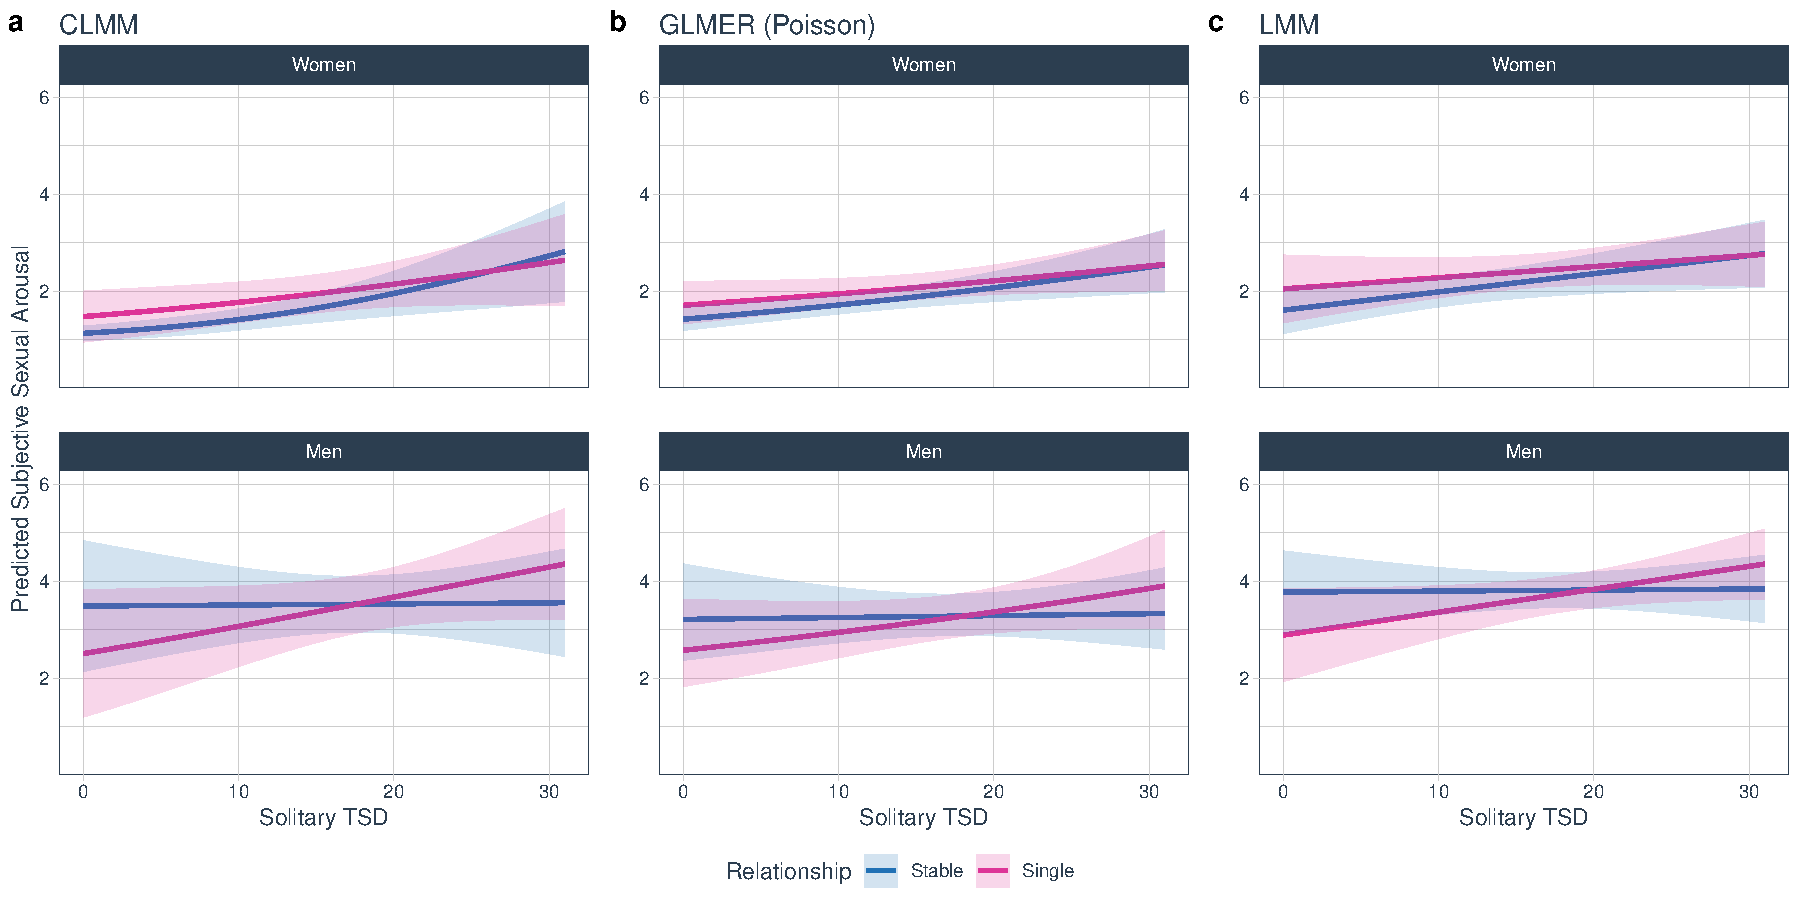
\includegraphics{Sexual_Desire_Arousal_anonymous_files/figure-latex/preds-m3a-1.pdf}
\caption{\label{fig:preds-m3a}Predicted subjective sexual arousal as a function of Solitary TSD, modeled using three statistical approaches: \textbf{(a)} Cumulative Link Mixed Model (CLMM); \textbf{(b)} Generalized Linear Mixed Model (GLMM) with a Poisson family; \textbf{(c)} Linear Mixed Model (LMM). Lines represent predicted values, and shaded areas indicate 95\% confidence intervals. The models include participant gender and relationship status as key factors.}
\end{figure}

\paragraph{Final Model: Effects of Solitary TSD on SSA Across Gender and Stimuli Sex}\label{final-model-effects-of-solitary-tsd-on-ssa-across-gender-and-stimuli-sex-1}

Given the apparent robustness of most results across models (CLMM, GLMER and LMM; Table \ref{tab:tab-robu-m3a}, Fig. \ref{fig:preds-m3a}), we test the predictions of the hypothesis from the LMM (\texttt{m3a\_lmer}).

\subparagraph{\texorpdfstring{Table \ref{tab:tab-m3a}. ANOVA-type table for the interaction between \texttt{Relationship\ type}, and \texttt{Gender}}{Table \ref{tab:tab-m3a}. ANOVA-type table for the interaction between Relationship type, and Gender}}\label{table-reftabtab-m3a.-anova-type-table-for-the-interaction-between-relationship-type-and-gender}

This tables summarizes the results of the model.

\begin{Shaded}
\begin{Highlighting}[]
\CommentTok{\# Generate ANOVA{-}type table for the final LMM model}
\CommentTok{\# This summarizes the effects of Solitary TSD on SSA across Gender and Relationship}
\FunctionTok{anova.sig.lmer}\NormalTok{(}
  \AttributeTok{model =}\NormalTok{ m3a\_lmer, }\CommentTok{\# Use LMM as the final model}
  \AttributeTok{custom\_caption =} \StringTok{"Effects of Solitary TSD on SSA Across Gender and Relationship"}
\NormalTok{)}
\end{Highlighting}
\end{Shaded}

\begin{table}[H]
\centering
\caption{\label{tab:tab-m3a}Effects of Solitary TSD on SSA Across Gender and Relationship}
\centering
\resizebox{\ifdim\width>\linewidth\linewidth\else\width\fi}{!}{
\begin{threeparttable}
\begin{tabular}[t]{lcccc}
\toprule
Effect & $df$ & $F$ & $p$ & $\epsilon^2_p$\\
\midrule
Solitary TSD & 1, 315 & 6.88 & \textbf{0.0091} & 0.0183\\
Gender & 1, 355.34 & 14.10 & \textbf{< 0.001} & 0.0355\\
Relationship & 1, 314.95 & 0.34 & 0.56 & < 0.0001\\
Solitary TSD × Gender & 1, 315.23 & 0.07 & 0.79 & < 0.0001\\
Solitary TSD × Relationship & 1, 314.95 & 0.53 & 0.47 & < 0.0001\\
Gender × Relationship & 1, 314.95 & 2.95 & 0.09 & 0.0061\\
Solitary TSD × Gender × Relationship & 1, 315.08 & 2.02 & 0.16 & 0.0032\\
\bottomrule
\end{tabular}
\begin{tablenotes}[para]
\item \textit{Note: } 
\item Results are Type III ANOVA. $R^2_{conditional}$ = 0.72, $R^2_{marginal}$ = 0.171. As effect size, we report partial epsilon squared ($\epsilon^2_p$), a less biased estimate than $\eta^2$ (see \cite{albersWhenPowerAnalyses2018}). Significant effects are in bold.
\end{tablenotes}
\end{threeparttable}}
\end{table}

\subparagraph{\texorpdfstring{\emph{Post-hoc} tests}{Post-hoc tests}}\label{post-hoc-tests-3}

To test the hypothesis, which predicted that there would be different relationship between SSA and solitary TSD, and that this association differ between men and women depending on the sex of stimuli, we used simple slope analysis.

\begin{Shaded}
\begin{Highlighting}[]
\CommentTok{\# Compute simple slopes for Solitary TSD on SSA, moderated by Gender and Relationship}
\NormalTok{slop.m3a\_lmer }\OtherTok{\textless{}{-}} \FunctionTok{sim\_slopes}\NormalTok{(m3a\_lmer,}
  \AttributeTok{pred =}\NormalTok{ Solitary.TSD, }\CommentTok{\# Predictor: Solitary TSD}
  \AttributeTok{modx =}\NormalTok{ Relationship, }\CommentTok{\# Moderator 1: Relationship status}
  \AttributeTok{mod2 =}\NormalTok{ Gender, }\CommentTok{\# Moderator 2: Gender}
  \AttributeTok{confint =} \ConstantTok{TRUE}
\NormalTok{) }\CommentTok{\# Compute confidence intervals}

\CommentTok{\# Extract slopes separately for Women and Men, then combine into a single table}
\NormalTok{slop.m3a\_lmer.tab }\OtherTok{\textless{}{-}} \FunctionTok{bind\_rows}\NormalTok{(}
\NormalTok{  slop.m3a\_lmer}\SpecialCharTok{$}\NormalTok{slopes[[}\DecValTok{1}\NormalTok{]] }\SpecialCharTok{|\textgreater{}}
    \FunctionTok{mutate}\NormalTok{(}\AttributeTok{Gender =} \StringTok{"Women"}\NormalTok{),}
\NormalTok{  slop.m3a\_lmer}\SpecialCharTok{$}\NormalTok{slopes[[}\DecValTok{2}\NormalTok{]] }\SpecialCharTok{|\textgreater{}}
    \FunctionTok{mutate}\NormalTok{(}\AttributeTok{Gender =} \StringTok{"Men"}\NormalTok{)}
\NormalTok{) }\SpecialCharTok{|\textgreater{}}
  \FunctionTok{mutate}\NormalTok{(}\AttributeTok{Gender =} \FunctionTok{recode\_factor}\NormalTok{(Gender,}
    \AttributeTok{Femenino =} \StringTok{"Women"}\NormalTok{,}
    \AttributeTok{Masculino =} \StringTok{"Men"}
\NormalTok{  )) }\SpecialCharTok{|\textgreater{}}
  \FunctionTok{select}\NormalTok{(}\DecValTok{8}\NormalTok{, }\DecValTok{1}\SpecialCharTok{:}\DecValTok{2}\NormalTok{, }\DecValTok{4}\SpecialCharTok{:}\DecValTok{7}\NormalTok{) }\SpecialCharTok{|\textgreater{}} \CommentTok{\# Select relevant columns}
  \FunctionTok{mutate}\NormalTok{(}\FunctionTok{across}\NormalTok{(}\DecValTok{3}\SpecialCharTok{:}\DecValTok{7}\NormalTok{, as.numeric)) }\SpecialCharTok{|\textgreater{}} \CommentTok{\# Ensure numeric format}
  \FunctionTok{mutate}\NormalTok{(}\FunctionTok{across}\NormalTok{(}\DecValTok{3}\SpecialCharTok{:}\DecValTok{6}\NormalTok{, round, }\DecValTok{2}\NormalTok{)) }\SpecialCharTok{|\textgreater{}} \CommentTok{\# Round coefficients and confidence intervals}
  \FunctionTok{mutate}\NormalTok{(}\AttributeTok{sig =} \FunctionTok{pval.stars}\NormalTok{(p)) }\SpecialCharTok{|\textgreater{}} \CommentTok{\# Add significance stars}
  \FunctionTok{rename}\NormalTok{(}\StringTok{"Relationship"} \OtherTok{=} \StringTok{"Value of Relationship"}\NormalTok{) }\SpecialCharTok{|\textgreater{}} \CommentTok{\# Rename columns for clarity}
  \FunctionTok{rename}\NormalTok{(}\AttributeTok{Coefficient =}\NormalTok{ Est.) }\CommentTok{\# Rename estimated coefficient column}

\CommentTok{\# Format and display the table using \textasciigrave{}kable\textasciigrave{}}
\NormalTok{slop.m3a\_lmer.tab[, }\SpecialCharTok{{-}}\FunctionTok{c}\NormalTok{(}\DecValTok{1}\NormalTok{, }\DecValTok{8}\NormalTok{)] }\SpecialCharTok{|\textgreater{}} \CommentTok{\# Remove first and eighth columns}
  \FunctionTok{mutate}\NormalTok{(}\AttributeTok{p =} \FunctionTok{pval.lev}\NormalTok{(p)) }\SpecialCharTok{|\textgreater{}} \CommentTok{\# Format p{-}values}
  \FunctionTok{kable}\NormalTok{(}
    \AttributeTok{booktabs =} \ConstantTok{TRUE}\NormalTok{,}
    \AttributeTok{align =} \FunctionTok{c}\NormalTok{(}\StringTok{"l"}\NormalTok{, }\FunctionTok{rep}\NormalTok{(}\StringTok{"c"}\NormalTok{, }\DecValTok{5}\NormalTok{)),}
    \AttributeTok{caption =} \StringTok{"Slope for Solitary TSD on}
\StringTok{        Subjective sexual arousal by relationship status and gender"}\NormalTok{,}
    \AttributeTok{linesep =} \StringTok{""}\NormalTok{,}
    \AttributeTok{col.names =} \FunctionTok{c}\NormalTok{(}
      \StringTok{"Relationship status"}\NormalTok{,}
      \StringTok{"$B$"}\NormalTok{,}
      \StringTok{"$2.5}\SpecialCharTok{\textbackslash{}\textbackslash{}}\StringTok{\% CI$"}\NormalTok{,}
      \StringTok{"$97.5}\SpecialCharTok{\textbackslash{}\textbackslash{}}\StringTok{\% CI$"}\NormalTok{,}
      \StringTok{"$t$"}\NormalTok{,}
      \StringTok{"$p$"}
\NormalTok{    ),}
    \AttributeTok{escape =} \ConstantTok{FALSE}
\NormalTok{  ) }\SpecialCharTok{|\textgreater{}}
  \FunctionTok{kable\_styling}\NormalTok{(}\AttributeTok{latex\_options =} \FunctionTok{c}\NormalTok{(}\StringTok{"HOLD\_position"}\NormalTok{)) }\SpecialCharTok{|\textgreater{}}
  \FunctionTok{pack\_rows}\NormalTok{(}
    \AttributeTok{group\_label =} \StringTok{"Gender: Women"}\NormalTok{,}
    \AttributeTok{start\_row =} \DecValTok{1}\NormalTok{,}
    \AttributeTok{end\_row =} \DecValTok{2}\NormalTok{,}
    \AttributeTok{bold =} \ConstantTok{FALSE}\NormalTok{,}
    \AttributeTok{background =} \StringTok{"lightgray"}
\NormalTok{  ) }\SpecialCharTok{|\textgreater{}}
  \FunctionTok{pack\_rows}\NormalTok{(}
    \AttributeTok{group\_label =} \StringTok{"Gender: Men"}\NormalTok{,}
    \AttributeTok{start\_row =} \DecValTok{3}\NormalTok{,}
    \AttributeTok{end\_row =} \DecValTok{4}\NormalTok{,}
    \AttributeTok{bold =} \ConstantTok{FALSE}\NormalTok{,}
    \AttributeTok{background =} \StringTok{"lightgray"}
\NormalTok{  ) }\SpecialCharTok{|\textgreater{}}
  \FunctionTok{footnote}\NormalTok{(}
    \AttributeTok{general =} \StringTok{"$B$ are unstandardized coefficients.}
\StringTok{           No intercept is reported as continuous predictors were centered}
\StringTok{           and are dependent on this specific sample."}\NormalTok{,}
    \AttributeTok{threeparttable =} \ConstantTok{TRUE}\NormalTok{,}
    \AttributeTok{footnote\_as\_chunk =} \ConstantTok{TRUE}\NormalTok{,}
    \AttributeTok{escape =} \ConstantTok{FALSE}
\NormalTok{  )}
\end{Highlighting}
\end{Shaded}

\begin{table}[H]
\centering
\caption{\label{tab:unnamed-chunk-28}Slope for Solitary TSD on
        Subjective sexual arousal by relationship status and gender}
\centering
\begin{threeparttable}
\begin{tabular}[t]{lccccc}
\toprule
Relationship status & $B$ & $2.5\% CI$ & $97.5\% CI$ & $t$ & $p$\\
\midrule
\addlinespace[0.3em]
\multicolumn{6}{l}{\cellcolor{lightgray}{Gender: Women}}\\
\hspace{1em}Stable & 0.04 & 0.01 & 0.07 & 2.31 & \textbf{0.0217}\\
\hspace{1em}Single & 0.02 & -0.01 & 0.06 & 1.19 & 0.23\\
\addlinespace[0.3em]
\multicolumn{6}{l}{\cellcolor{lightgray}{Gender: Men}}\\
\hspace{1em}Stable & 0.00 & -0.04 & 0.05 & 0.10 & 0.92\\
\hspace{1em}Single & 0.05 & 0.00 & 0.10 & 1.91 & 0.06\\
\bottomrule
\end{tabular}
\begin{tablenotes}[para]
\item \textit{Note: } 
\item $B$ are unstandardized coefficients.
           No intercept is reported as continuous predictors were centered
           and are dependent on this specific sample.
\end{tablenotes}
\end{threeparttable}
\end{table}

\paragraph{Figure \ref{fig:fig-h3a}. Subjective sexual arousal to erotic stimuli: Main effects and interactions}\label{figure-reffigfig-h3a.-subjective-sexual-arousal-to-erotic-stimuli-main-effects-and-interactions}

This figure summarizes the results of hypothesis 3a.

\begin{Shaded}
\begin{Highlighting}[]
\CommentTok{\# Generate final plot for Solitary TSD effects on SSA}
\CommentTok{\# Includes interaction between Relationship status and Gender}
\NormalTok{p\_m3a.fin }\OtherTok{\textless{}{-}}\NormalTok{ p\_m3a\_lmer }\SpecialCharTok{+}
  \FunctionTok{labs}\NormalTok{(}
    \AttributeTok{title =} \StringTok{""}\NormalTok{,}
    \AttributeTok{y =} \StringTok{"Predicted Subjective Sexual Arousal"}
\NormalTok{  ) }\SpecialCharTok{+}
  \FunctionTok{facet\_wrap}\NormalTok{(}\SpecialCharTok{\textasciitilde{}}\NormalTok{Gender, }\AttributeTok{ncol =} \DecValTok{2}\NormalTok{) }\SpecialCharTok{+} \CommentTok{\# Separate plots by Gender}

  \CommentTok{\# Add text labels with regression coefficients, confidence intervals, and p{-}values}
  \FunctionTok{geom\_text}\NormalTok{(}
    \AttributeTok{data =}\NormalTok{ slop.m3a\_lmer.tab }\SpecialCharTok{|\textgreater{}}
      \FunctionTok{mutate}\NormalTok{(}\AttributeTok{Solitary.TSD =} \DecValTok{2}\NormalTok{), }\CommentTok{\# Assign a reference value for positioning}
    \AttributeTok{mapping =} \FunctionTok{aes}\NormalTok{(}
      \AttributeTok{x =} \FunctionTok{min}\NormalTok{(Solitary.TSD), }\AttributeTok{y =} \ConstantTok{Inf}\NormalTok{,}
      \AttributeTok{label =} \FunctionTok{paste}\NormalTok{(}
        \StringTok{"B = "}\NormalTok{, Coefficient,}
        \StringTok{", IC 95\%["}\NormalTok{, }\StringTok{\textasciigrave{}}\AttributeTok{2.5\%}\StringTok{\textasciigrave{}}\NormalTok{, }\StringTok{", "}\NormalTok{, }\StringTok{\textasciigrave{}}\AttributeTok{97.5\%}\StringTok{\textasciigrave{}}\NormalTok{,}
        \StringTok{"], p"}\NormalTok{,}
        \FunctionTok{ifelse}\NormalTok{(}\FunctionTok{grepl}\NormalTok{(}\StringTok{"\textless{}"}\NormalTok{, }\FunctionTok{pe2.lev}\NormalTok{(p)), }\FunctionTok{pe2.lev}\NormalTok{(p),}
          \FunctionTok{paste0}\NormalTok{(}\StringTok{" = "}\NormalTok{, }\FunctionTok{pe2.lev}\NormalTok{(p))}
\NormalTok{        ),}
        \FunctionTok{ifelse}\NormalTok{(}\FunctionTok{is.na}\NormalTok{(sig), }\StringTok{""}\NormalTok{, sig)}
\NormalTok{      ),}
      \AttributeTok{vjust =} \DecValTok{2} \SpecialCharTok{+} \FunctionTok{as.numeric}\NormalTok{(}\FunctionTok{as.factor}\NormalTok{(Relationship)) }\SpecialCharTok{*} \DecValTok{2}
\NormalTok{    ),}
    \CommentTok{\# Adjust vertical positioning based on Relationship status}
    \AttributeTok{hjust =} \SpecialCharTok{{-}}\FloatTok{0.1}\NormalTok{, }\CommentTok{\# Left{-}align text labels}
    \AttributeTok{show.legend =} \ConstantTok{FALSE}
\NormalTok{  ) }\SpecialCharTok{+} \CommentTok{\# Hide legend for text labels}

  \FunctionTok{theme}\NormalTok{(}\AttributeTok{legend.position =} \StringTok{"bottom"}\NormalTok{) }\CommentTok{\# Move legend to bottom}

\CommentTok{\# Display the final plot}
\NormalTok{p\_m3a.fin}
\end{Highlighting}
\end{Shaded}

\begin{figure}
\centering
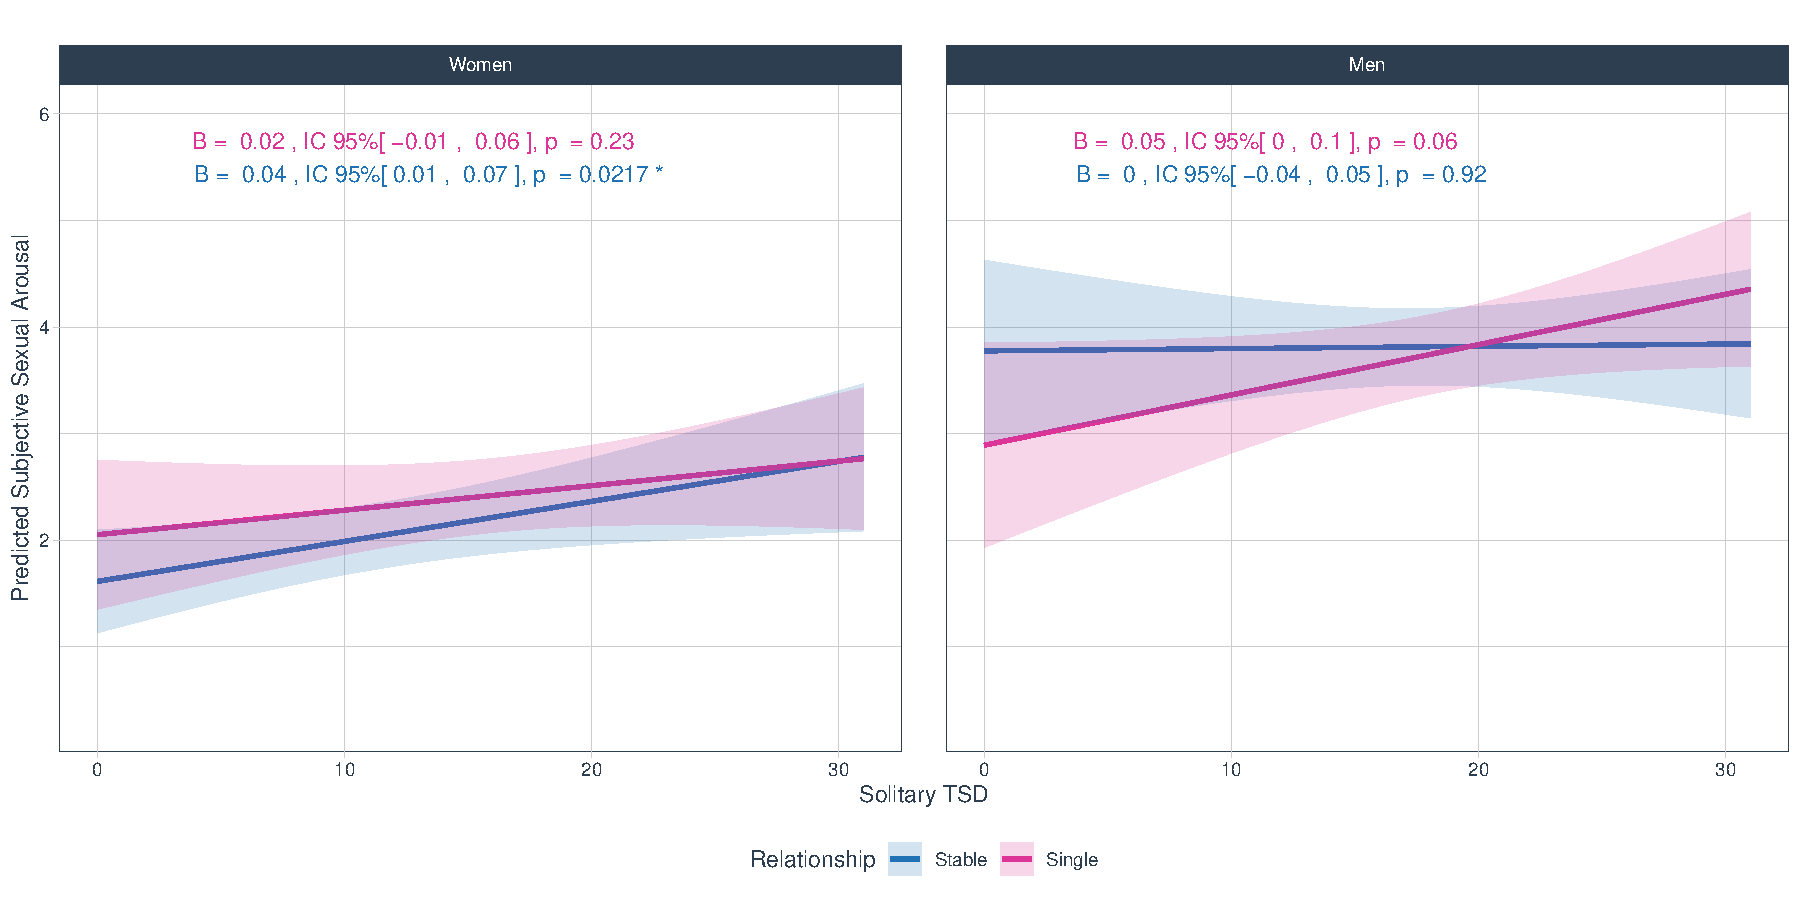
\includegraphics{Sexual_Desire_Arousal_anonymous_files/figure-latex/fig-h3a-1.pdf}
\caption{\label{fig:fig-h3a}Predicted subjective sexual arousal as a function of Solitary TSD, modeled using aLinear Mixed Model (LMM). Lines represent predicted values, and shaded areas indicate 95\% confidence intervals. The model include participant gender and relationship status as key factors.}
\end{figure}

\subsubsection{Hypothesis 3b: Dyadic TSD Attractive Person}\label{hyp3b}

\paragraph{Model Robustness: Examining the Effects of Dyadic TSD Attractive Person on SSA Across Gender and Stimuli Sex}\label{model-robustness-examining-the-effects-of-dyadic-tsd-attractive-person-on-ssa-across-gender-and-stimuli-sex-1}

To assess the robustness of our findings, we fitted three different models examining how Dyadic TSD Attractive Person predicts SSA, considering variations by gender and stimuli sex:

\begin{enumerate}
\def\labelenumi{\arabic{enumi}.}
\tightlist
\item
  Cumulative Link Mixed Model (CLMM) -- \texttt{m3b\_clmm} (for ordinal outcomes, using a probit link).
\item
  Generalized Linear Mixed Model (GLMM) with Poisson family -- \texttt{m3b\_poisson} (treating SSA as a count variable).
\item
  Linear Mixed Model (LMM) -- \texttt{m3b\_lmer} (treating SSA as a continuous variable).
\end{enumerate}

\begin{Shaded}
\begin{Highlighting}[]
\CommentTok{\# Fit three different models to assess robustness of Dyadic TSD Attractive Person on SSA}

\CommentTok{\# (1) Cumulative Link Mixed Model (CLMM) {-} Ordinal model with probit link}
\NormalTok{m3b\_clmm }\OtherTok{\textless{}{-}} \FunctionTok{clmm}\NormalTok{(}
\NormalTok{  Subjective.sexual.arousal.factor }\SpecialCharTok{\textasciitilde{}}\NormalTok{ Dyadic.TSD.Attractive.Person }\SpecialCharTok{*}\NormalTok{ Gender }\SpecialCharTok{*}\NormalTok{ Relationship }\SpecialCharTok{+}
\NormalTok{    (}\DecValTok{1} \SpecialCharTok{|}\NormalTok{ Stimuli.code) }\SpecialCharTok{+} \CommentTok{\# Random intercept for Stimuli}
\NormalTok{    (}\DecValTok{1} \SpecialCharTok{|}\NormalTok{ Participant), }\CommentTok{\# Random intercept \& slope for Relationship status}
  \AttributeTok{data =}\NormalTok{ dat\_m3,}
  \AttributeTok{link =} \StringTok{"probit"}\NormalTok{, }\CommentTok{\# Use probit link for ordinal regression}
  \AttributeTok{control =} \FunctionTok{list}\NormalTok{(}\AttributeTok{method =} \StringTok{"nlminb"}\NormalTok{) }\CommentTok{\# Use \textquotesingle{}nlminb\textquotesingle{} optimizer for better convergence}
\NormalTok{)}

\CommentTok{\# (2) Generalized Linear Mixed Model (GLMM) {-} Poisson regression for count data}
\NormalTok{m3b\_poisson }\OtherTok{\textless{}{-}} \FunctionTok{glmer}\NormalTok{(}
\NormalTok{  Subjective.sexual.arousal }\SpecialCharTok{\textasciitilde{}}\NormalTok{ Dyadic.TSD.Attractive.Person }\SpecialCharTok{*}\NormalTok{ Gender }\SpecialCharTok{*}\NormalTok{ Relationship }\SpecialCharTok{+}
\NormalTok{    (}\DecValTok{1} \SpecialCharTok{|}\NormalTok{ Stimuli.code) }\SpecialCharTok{+} \CommentTok{\# Random intercept for Stimuli}
\NormalTok{    (}\DecValTok{1} \SpecialCharTok{|}\NormalTok{ Participant), }\CommentTok{\# Random intercept \& slope for Relationship status}
  \AttributeTok{data =}\NormalTok{ dat\_m3,}
  \AttributeTok{family =}\NormalTok{ poisson }\CommentTok{\# Poisson distribution for count data}
\NormalTok{)}

\CommentTok{\# (3) Linear Mixed Model (LMM) {-} Continuous approximation}
\NormalTok{m3b\_lmer }\OtherTok{\textless{}{-}} \FunctionTok{lmer}\NormalTok{(}
\NormalTok{  Subjective.sexual.arousal }\SpecialCharTok{\textasciitilde{}}\NormalTok{ Dyadic.TSD.Attractive.Person }\SpecialCharTok{*}\NormalTok{ Gender }\SpecialCharTok{*}\NormalTok{ Relationship }\SpecialCharTok{+}
\NormalTok{    (}\DecValTok{1} \SpecialCharTok{|}\NormalTok{ Stimuli.code) }\SpecialCharTok{+} \CommentTok{\# Random intercept for Stimuli}
\NormalTok{    (}\DecValTok{1} \SpecialCharTok{|}\NormalTok{ Participant), }\CommentTok{\# Random intercept \& slope for Relationship status}
  \AttributeTok{data =}\NormalTok{ dat\_m3,}
  \AttributeTok{control =} \FunctionTok{lmerControl}\NormalTok{(}\AttributeTok{optimizer =} \StringTok{"bobyqa"}\NormalTok{) }\CommentTok{\# Use \textquotesingle{}bobyqa\textquotesingle{} optimizer for stability}
\NormalTok{)}
\end{Highlighting}
\end{Shaded}

\subparagraph{Table \ref{tab:tab-robu-m3b}. ANOVA-type table of fixed effects (main effects and interactions) across the three fitted models}\label{table-reftabtab-robu-m3b.-anova-type-table-of-fixed-effects-main-effects-and-interactions-across-the-three-fitted-models}

As shown in the table below, the pattern of significant effects remains consistent across all three models, except for the main effect of gender, which is not significant in the CLMM.

\begin{Shaded}
\begin{Highlighting}[]
\CommentTok{\# Compare fixed effects across CLMM, GLMM, and LMM models for Hypothesis 3b}
\CommentTok{\# This function generates an ANOVA{-}type table summarizing main effects and interactions}
\FunctionTok{anova.comp}\NormalTok{(}
  \AttributeTok{CLMMmod =}\NormalTok{ m3b\_clmm, }\CommentTok{\# Cumulative Link Mixed Model (CLMM)}
  \AttributeTok{GLMERmod =}\NormalTok{ m3b\_poisson, }\CommentTok{\# Generalized Linear Mixed Model (GLMM, Poisson)}
  \AttributeTok{LMERmod =}\NormalTok{ m3b\_lmer, }\CommentTok{\# Linear Mixed Model (LMM)}
  \AttributeTok{hypothesis =} \StringTok{"3b"} \CommentTok{\# Hypothesis identifier for documentation purposes}
\NormalTok{)}
\end{Highlighting}
\end{Shaded}

\begin{table}[H]
\centering
\caption{\label{tab:tab-robu-m3b}Comparison of fixed effects across the three models for Hypothesis 3b: CLMM, GLMM (Poisson), and LMM.}
\centering
\resizebox{\ifdim\width>\linewidth\linewidth\else\width\fi}{!}{
\begin{threeparttable}
\begin{tabular}[t]{lccccccccc}
\toprule
\multicolumn{1}{c}{ } & \multicolumn{3}{c}{CLMM} & \multicolumn{3}{c}{GLMER (Poisson)} & \multicolumn{3}{c}{LMM} \\
\cmidrule(l{3pt}r{3pt}){2-4} \cmidrule(l{3pt}r{3pt}){5-7} \cmidrule(l{3pt}r{3pt}){8-10}
Effect & $df$ & $\chi^2$ & $p$ & $df$ & $\chi^2$ & $p$ & $df$ & $F$ & $p$\\
\midrule
Dyadic TSD Attractive Person & 1 & 47.486 & \textbf{< 0.0001} & 1 & 47.634 & \textbf{< 0.0001} & 1, 315.21 & 46.796 & \textbf{< 0.0001}\\
Gender & 1 & 4.636 & \textbf{0.0313} & 1 & 4.229 & \textbf{0.0397} & 1, 354.77 & 1.207 & 0.27\\
Relationship & 1 & 0.928 & 0.34 & 1 & 0.353 & 0.55 & 1, 315.16 & 0.126 & 0.72\\
Dyadic TSD Attractive Person × Gender & 1 & 0.452 & 0.5 & 1 & 1.391 & 0.24 & 1, 314.97 & 7.064 & \textbf{0.0083}\\
Dyadic TSD Attractive Person × Relationship & 1 & 0.525 & 0.47 & 1 & 0.130 & 0.72 & 1, 315.21 & 0.084 & 0.77\\
Gender × Relationship & 1 & 0.000 & 0.99 & 1 & 0.005 & 0.94 & 1, 315.06 & 0.001 & 0.97\\
Dyadic TSD Attractive Person × Gender × Relationship & 1 & 0.215 & 0.64 & 1 & 0.213 & 0.64 & 1, 314.97 & 0.339 & 0.56\\
\bottomrule
\end{tabular}
\begin{tablenotes}[para]
\item \textit{Note: } 
\item For CLMM and GLMER (Poisson) models, results are
              Analysis of Deviance (Type III Wald chi-square tests),
              while for LMM, results are from an Analysis of Variance
              (Type III ANOVA with Satterthwaite's method).
              Significant effects are in bold.
\end{tablenotes}
\end{threeparttable}}
\end{table}

\subparagraph{Figure \ref{fig:preds-m3b}: Model-based predictions for Hypothesis 3b.}\label{figure-reffigpreds-m3b-model-based-predictions-for-hypothesis-3b.}

This figure presents model-based predictions of subjective sexual arousal as a function of Dyadic TSD Attractive Person, across different relationship status and participant genders. The three subplots correspond to the three statistical models used for analysis: (a) Cumulative Link Mixed Model (CLMM), (b) Generalized Linear Mixed Model (GLMM, Poisson), and (c) Linear Mixed Model (LMM). Shaded areas represent 95\% confidence intervals.

\begin{Shaded}
\begin{Highlighting}[]
\CommentTok{\# Generate model{-}based predictions for Hypothesis 3b}
\CommentTok{\# Predict SSA based on Dyadic TSD Attractive Person across gender and relationship status}

\CommentTok{\# CLMM Predictions}
\NormalTok{p\_m3b\_clmm }\OtherTok{\textless{}{-}} \FunctionTok{emmeans}\NormalTok{(m3b\_clmm, }\SpecialCharTok{\textasciitilde{}}\NormalTok{ Dyadic.TSD.Attractive.Person }\SpecialCharTok{|}\NormalTok{ Gender }\SpecialCharTok{*}\NormalTok{ Relationship,}
  \AttributeTok{at =} \FunctionTok{list}\NormalTok{(}\AttributeTok{Dyadic.TSD.Attractive.Person =} \FunctionTok{seq}\NormalTok{(}\DecValTok{0}\NormalTok{, }\DecValTok{31}\NormalTok{, }\AttributeTok{length.out =} \DecValTok{100}\NormalTok{)),}
  \AttributeTok{mode =} \StringTok{"mean.class"} \CommentTok{\# Compute predicted mean response categories}
\NormalTok{) }\SpecialCharTok{|\textgreater{}}
  \FunctionTok{as.data.frame}\NormalTok{() }\SpecialCharTok{|\textgreater{}} \CommentTok{\# Convert predictions to a dataframe for ggplot}
  \FunctionTok{ggplot}\NormalTok{(}\FunctionTok{aes}\NormalTok{(}
    \AttributeTok{x =}\NormalTok{ Dyadic.TSD.Attractive.Person, }\AttributeTok{y =}\NormalTok{ mean.class,}
    \AttributeTok{color =}\NormalTok{ Relationship, }\AttributeTok{fill =}\NormalTok{ Relationship}
\NormalTok{  )) }\SpecialCharTok{+}
  \FunctionTok{geom\_line}\NormalTok{(}\AttributeTok{size =} \DecValTok{1}\NormalTok{) }\SpecialCharTok{+} \CommentTok{\# Plot predicted response line}
  \FunctionTok{geom\_ribbon}\NormalTok{(}\FunctionTok{aes}\NormalTok{(}\AttributeTok{ymin =}\NormalTok{ asymp.LCL, }\AttributeTok{ymax =}\NormalTok{ asymp.UCL, }\AttributeTok{fill =}\NormalTok{ Relationship),}
    \AttributeTok{alpha =} \FloatTok{0.2}\NormalTok{, }\AttributeTok{color =} \ConstantTok{NA} \CommentTok{\# Add confidence interval as shaded ribbon}
\NormalTok{  ) }\SpecialCharTok{+}
  \FunctionTok{scale\_color\_manual}\NormalTok{(}\AttributeTok{values =}\NormalTok{ color.Relationship) }\SpecialCharTok{+} \CommentTok{\# Apply custom colors}
  \FunctionTok{scale\_fill\_manual}\NormalTok{(}\AttributeTok{values =}\NormalTok{ color.Relationship) }\SpecialCharTok{+}
  \FunctionTok{facet\_wrap}\NormalTok{(}\SpecialCharTok{\textasciitilde{}}\NormalTok{Gender, }\AttributeTok{ncol =} \DecValTok{1}\NormalTok{) }\SpecialCharTok{+} \CommentTok{\# Create separate plots for each gender}
  \FunctionTok{labs}\NormalTok{(}
    \AttributeTok{y =} \StringTok{"Predicted Subjective Sexual Arousal"}\NormalTok{, }\AttributeTok{x =} \StringTok{"Attractive Person Sexual Desire"}\NormalTok{,}
    \AttributeTok{title =} \StringTok{"CLMM"}
\NormalTok{  ) }\SpecialCharTok{+}
  \FunctionTok{theme\_tq}\NormalTok{() }\SpecialCharTok{+} \CommentTok{\# Apply custom theme}
  \FunctionTok{theme}\NormalTok{(}\AttributeTok{legend.position =} \StringTok{"bottom"}\NormalTok{) }\SpecialCharTok{+}
  \FunctionTok{ylim}\NormalTok{(}\FunctionTok{c}\NormalTok{(}\FloatTok{0.3}\NormalTok{, }\DecValTok{7}\NormalTok{)) }\CommentTok{\# Set Y{-}axis limits}

\CommentTok{\# Poisson GLMM Predictions}
\NormalTok{p\_m3b\_poisson }\OtherTok{\textless{}{-}} \FunctionTok{emmeans}\NormalTok{(m3b\_poisson, }\SpecialCharTok{\textasciitilde{}}\NormalTok{ Dyadic.TSD.Attractive.Person }\SpecialCharTok{|}\NormalTok{ Gender }\SpecialCharTok{*}\NormalTok{ Relationship,}
  \AttributeTok{at =} \FunctionTok{list}\NormalTok{(}\AttributeTok{Dyadic.TSD.Attractive.Person =} \FunctionTok{seq}\NormalTok{(}\DecValTok{0}\NormalTok{, }\DecValTok{31}\NormalTok{, }\AttributeTok{length.out =} \DecValTok{100}\NormalTok{)),}
  \AttributeTok{type =} \StringTok{"response"} \CommentTok{\# Compute response{-}scale predictions}
\NormalTok{) }\SpecialCharTok{|\textgreater{}}
  \FunctionTok{as.data.frame}\NormalTok{() }\SpecialCharTok{|\textgreater{}}
  \FunctionTok{ggplot}\NormalTok{(}\FunctionTok{aes}\NormalTok{(}
    \AttributeTok{x =}\NormalTok{ Dyadic.TSD.Attractive.Person, }\AttributeTok{y =}\NormalTok{ rate,}
    \AttributeTok{color =}\NormalTok{ Relationship, }\AttributeTok{fill =}\NormalTok{ Relationship}
\NormalTok{  )) }\SpecialCharTok{+}
  \FunctionTok{geom\_line}\NormalTok{(}\AttributeTok{size =} \DecValTok{1}\NormalTok{) }\SpecialCharTok{+}
  \FunctionTok{geom\_ribbon}\NormalTok{(}\FunctionTok{aes}\NormalTok{(}\AttributeTok{ymin =}\NormalTok{ asymp.LCL, }\AttributeTok{ymax =}\NormalTok{ asymp.UCL, }\AttributeTok{fill =}\NormalTok{ Relationship),}
    \AttributeTok{alpha =} \FloatTok{0.2}\NormalTok{, }\AttributeTok{color =} \ConstantTok{NA}
\NormalTok{  ) }\SpecialCharTok{+}
  \FunctionTok{scale\_color\_manual}\NormalTok{(}\AttributeTok{values =}\NormalTok{ color.Relationship) }\SpecialCharTok{+}
  \FunctionTok{scale\_fill\_manual}\NormalTok{(}\AttributeTok{values =}\NormalTok{ color.Relationship) }\SpecialCharTok{+}
  \FunctionTok{facet\_wrap}\NormalTok{(}\SpecialCharTok{\textasciitilde{}}\NormalTok{Gender, }\AttributeTok{ncol =} \DecValTok{1}\NormalTok{) }\SpecialCharTok{+}
  \FunctionTok{labs}\NormalTok{(}
    \AttributeTok{y =} \StringTok{""}\NormalTok{, }\AttributeTok{x =} \StringTok{"Attractive Person Sexual Desire"}\NormalTok{,}
    \AttributeTok{title =} \StringTok{"GLMER (Poisson)"}
\NormalTok{  ) }\SpecialCharTok{+}
  \FunctionTok{theme\_tq}\NormalTok{() }\SpecialCharTok{+}
  \FunctionTok{theme}\NormalTok{(}\AttributeTok{legend.position =} \StringTok{"bottom"}\NormalTok{) }\SpecialCharTok{+}
  \FunctionTok{ylim}\NormalTok{(}\FunctionTok{c}\NormalTok{(}\FloatTok{0.3}\NormalTok{, }\DecValTok{7}\NormalTok{))}

\CommentTok{\# LMM Predictions}
\NormalTok{p\_m3b\_lmer }\OtherTok{\textless{}{-}} \FunctionTok{emmeans}\NormalTok{(m3b\_lmer, }\SpecialCharTok{\textasciitilde{}}\NormalTok{ Dyadic.TSD.Attractive.Person }\SpecialCharTok{|}\NormalTok{ Gender }\SpecialCharTok{*}\NormalTok{ Relationship,}
  \AttributeTok{at =} \FunctionTok{list}\NormalTok{(}\AttributeTok{Dyadic.TSD.Attractive.Person =} \FunctionTok{seq}\NormalTok{(}\DecValTok{0}\NormalTok{, }\DecValTok{31}\NormalTok{, }\AttributeTok{length.out =} \DecValTok{100}\NormalTok{)),}
  \AttributeTok{type =} \StringTok{"response"}
\NormalTok{) }\SpecialCharTok{|\textgreater{}}
  \FunctionTok{as.data.frame}\NormalTok{() }\SpecialCharTok{|\textgreater{}}
  \FunctionTok{ggplot}\NormalTok{(}\FunctionTok{aes}\NormalTok{(}
    \AttributeTok{x =}\NormalTok{ Dyadic.TSD.Attractive.Person, }\AttributeTok{y =}\NormalTok{ emmean,}
    \AttributeTok{color =}\NormalTok{ Relationship, }\AttributeTok{fill =}\NormalTok{ Relationship}
\NormalTok{  )) }\SpecialCharTok{+}
  \FunctionTok{geom\_line}\NormalTok{(}\AttributeTok{size =} \DecValTok{1}\NormalTok{) }\SpecialCharTok{+}
  \FunctionTok{geom\_ribbon}\NormalTok{(}\FunctionTok{aes}\NormalTok{(}\AttributeTok{ymin =}\NormalTok{ asymp.LCL, }\AttributeTok{ymax =}\NormalTok{ asymp.UCL, }\AttributeTok{fill =}\NormalTok{ Relationship),}
    \AttributeTok{alpha =} \FloatTok{0.2}\NormalTok{, }\AttributeTok{color =} \ConstantTok{NA}
\NormalTok{  ) }\SpecialCharTok{+}
  \FunctionTok{scale\_color\_manual}\NormalTok{(}\AttributeTok{values =}\NormalTok{ color.Relationship) }\SpecialCharTok{+}
  \FunctionTok{scale\_fill\_manual}\NormalTok{(}\AttributeTok{values =}\NormalTok{ color.Relationship) }\SpecialCharTok{+}
  \FunctionTok{facet\_wrap}\NormalTok{(}\SpecialCharTok{\textasciitilde{}}\NormalTok{Gender, }\AttributeTok{ncol =} \DecValTok{1}\NormalTok{) }\SpecialCharTok{+}
  \FunctionTok{labs}\NormalTok{(}
    \AttributeTok{y =} \StringTok{""}\NormalTok{, }\AttributeTok{x =} \StringTok{"Attractive Person Sexual Desire"}\NormalTok{,}
    \AttributeTok{title =} \StringTok{"LMM"}
\NormalTok{  ) }\SpecialCharTok{+}
  \FunctionTok{theme\_tq}\NormalTok{() }\SpecialCharTok{+}
  \FunctionTok{theme}\NormalTok{(}\AttributeTok{legend.position =} \StringTok{"bottom"}\NormalTok{) }\SpecialCharTok{+}
  \FunctionTok{ylim}\NormalTok{(}\FunctionTok{c}\NormalTok{(}\FloatTok{0.3}\NormalTok{, }\DecValTok{7}\NormalTok{))}

\CommentTok{\# Arrange Plots into a Single Figure}
\NormalTok{p\_robu\_m3b }\OtherTok{\textless{}{-}} \FunctionTok{ggarrange}\NormalTok{(p\_m3b\_clmm, p\_m3b\_poisson, p\_m3b\_lmer, }\CommentTok{\# Combine plots side by side}
  \AttributeTok{common.legend =} \ConstantTok{TRUE}\NormalTok{, }\CommentTok{\# Share legend across plots}
  \AttributeTok{labels =} \StringTok{"auto"}\NormalTok{, }\CommentTok{\# Automatically label subfigures (a, b, c)}
  \AttributeTok{legend =} \StringTok{"bottom"}\NormalTok{,}
  \AttributeTok{nrow =} \DecValTok{1} \CommentTok{\# Arrange in a single row}
\NormalTok{)}

\CommentTok{\# Display the combined figure}
\NormalTok{p\_robu\_m3b}
\end{Highlighting}
\end{Shaded}

\begin{figure}
\centering
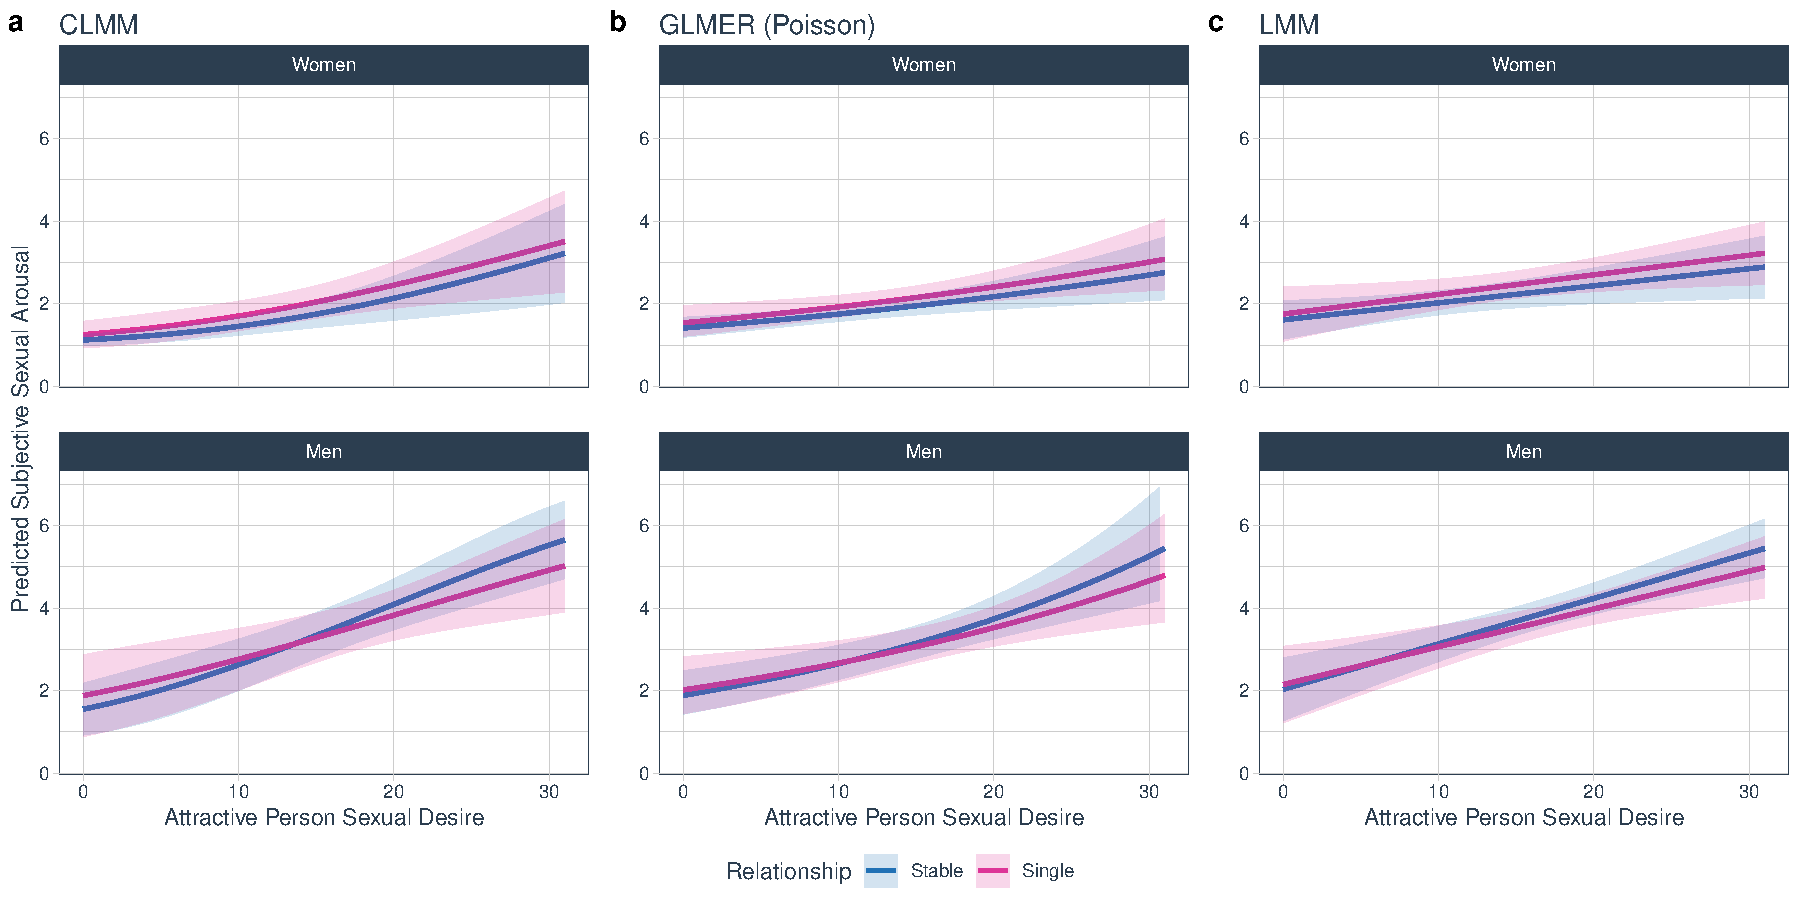
\includegraphics{Sexual_Desire_Arousal_anonymous_files/figure-latex/preds-m3b-1.pdf}
\caption{\label{fig:preds-m3b}Predicted subjective sexual arousal as a function of Dyadic TSD Attractive Person, modeled using three statistical approaches: \textbf{(a)} Cumulative Link Mixed Model (CLMM); \textbf{(b)} Generalized Linear Mixed Model (GLMM) with a Poisson family; \textbf{(c)} Linear Mixed Model (LMM). Lines represent predicted values, and shaded areas indicate 95\% confidence intervals. The models include participant gender and relationship status as key factors.}
\end{figure}

\paragraph{Final Model: Effects of Dyadic TSD Attractive Person on SSA Across Gender and Stimuli Sex}\label{final-model-effects-of-dyadic-tsd-attractive-person-on-ssa-across-gender-and-stimuli-sex-1}

Given the apparent robustness of most results across models (CLMM, GLMER and LMM; Table \ref{tab:tab-robu-m3b}, Fig. \ref{fig:preds-m3b}), we test the predictions of the hypothesis from the LMM (\texttt{m3b\_lmer}).

\subparagraph{\texorpdfstring{Table \ref{tab:tab-m3b}. ANOVA-type table for the interaction between \texttt{Relationship\ type}, and \texttt{Gender}}{Table \ref{tab:tab-m3b}. ANOVA-type table for the interaction between Relationship type, and Gender}}\label{table-reftabtab-m3b.-anova-type-table-for-the-interaction-between-relationship-type-and-gender}

This tables summarizes the results of the model.

\begin{Shaded}
\begin{Highlighting}[]
\CommentTok{\# Generate ANOVA{-}type table for the final LMM model}
\CommentTok{\# This summarizes the effects of Dyadic TSD Attractive Person on SSA}
\CommentTok{\# across Gender and Relationship Status}
\FunctionTok{anova.sig.lmer}\NormalTok{(}
  \AttributeTok{model =}\NormalTok{ m3b\_lmer, }\CommentTok{\# Use LMM as the final model}
  \AttributeTok{custom\_caption =} \StringTok{"Effects of Dyadic TSD Attractive Person on SSA }
\StringTok{  Across Gender and Stimuli Sex"}
\NormalTok{)}
\end{Highlighting}
\end{Shaded}

\begin{table}[H]
\centering
\caption{\label{tab:tab-m3b}Effects of Dyadic TSD Attractive Person on SSA 
  Across Gender and Stimuli Sex}
\centering
\resizebox{\ifdim\width>\linewidth\linewidth\else\width\fi}{!}{
\begin{threeparttable}
\begin{tabular}[t]{lcccc}
\toprule
Effect & $df$ & $F$ & $p$ & $\epsilon^2_p$\\
\midrule
Dyadic TSD Attractive Person & 1, 315.21 & 46.80 & \textbf{< 0.0001} & 0.13\\
Gender & 1, 354.77 & 1.21 & 0.27 & < 0.001\\
Relationship & 1, 315.16 & 0.13 & 0.72 & < 0.0001\\
Dyadic TSD Attractive Person × Gender & 1, 314.97 & 7.06 & \textbf{0.0083} & 0.0188\\
Dyadic TSD Attractive Person × Relationship & 1, 315.21 & 0.08 & 0.77 & < 0.0001\\
Gender × Relationship & 1, 315.06 & 0.00 & 0.97 & < 0.0001\\
Dyadic TSD Attractive Person × Gender × Relationship & 1, 314.97 & 0.34 & 0.56 & < 0.0001\\
\bottomrule
\end{tabular}
\begin{tablenotes}[para]
\item \textit{Note: } 
\item Results are Type III ANOVA. $R^2_{conditional}$ = 0.719, $R^2_{marginal}$ = 0.225. As effect size, we report partial epsilon squared ($\epsilon^2_p$), a less biased estimate than $\eta^2$ (see \cite{albersWhenPowerAnalyses2018}). Significant effects are in bold.
\end{tablenotes}
\end{threeparttable}}
\end{table}

\subparagraph{\texorpdfstring{\emph{Post-hoc} tests}{Post-hoc tests}}\label{post-hoc-tests-4}

To test the hypothesis, which predicted that there would be different relationship between SSA and Dyadic TSD Attractive Person, and that this association differ between men and women depending on the sex of stimuli, we used simple slope analysis.

\begin{Shaded}
\begin{Highlighting}[]
\CommentTok{\# Perform simple slopes analysis to examine the effect of Dyadic TSD Attractive Person}
\CommentTok{\# on SSA across Gender and Relationship Status}
\NormalTok{slop.m3b\_lmer }\OtherTok{\textless{}{-}} \FunctionTok{sim\_slopes}\NormalTok{(m3b\_lmer,}
  \AttributeTok{pred =}\NormalTok{ Dyadic.TSD.Attractive.Person, }\CommentTok{\# Predictor variable}
  \AttributeTok{modx =}\NormalTok{ Relationship, }\CommentTok{\# Moderator 1: Relationship status}
  \AttributeTok{mod2 =}\NormalTok{ Gender, }\CommentTok{\# Moderator 2: Gender}
  \AttributeTok{confint =} \ConstantTok{TRUE}
\NormalTok{) }\CommentTok{\# Compute confidence intervals}

\CommentTok{\# Combine slopes for Women and Men into a single dataframe for easier processing}
\NormalTok{slop.m3b\_lmer.tab }\OtherTok{\textless{}{-}} \FunctionTok{bind\_rows}\NormalTok{(}
\NormalTok{  slop.m3b\_lmer}\SpecialCharTok{$}\NormalTok{slopes[[}\DecValTok{1}\NormalTok{]] }\SpecialCharTok{|\textgreater{}}
    \FunctionTok{mutate}\NormalTok{(}\AttributeTok{Gender =} \StringTok{"Women"}\NormalTok{),}
\NormalTok{  slop.m3b\_lmer}\SpecialCharTok{$}\NormalTok{slopes[[}\DecValTok{2}\NormalTok{]] }\SpecialCharTok{|\textgreater{}}
    \FunctionTok{mutate}\NormalTok{(}\AttributeTok{Gender =} \StringTok{"Men"}\NormalTok{)}
\NormalTok{) }\SpecialCharTok{|\textgreater{}}
  \CommentTok{\# Recoding Gender labels to ensure consistency}
  \FunctionTok{mutate}\NormalTok{(}\AttributeTok{Gender =} \FunctionTok{recode\_factor}\NormalTok{(Gender, }\AttributeTok{Femenino =} \StringTok{"Women"}\NormalTok{, }\AttributeTok{Masculino =} \StringTok{"Men"}\NormalTok{)) }\SpecialCharTok{|\textgreater{}}
  \CommentTok{\# Select relevant columns (drop unnecessary ones)}
  \FunctionTok{select}\NormalTok{(}\DecValTok{8}\NormalTok{, }\DecValTok{1}\SpecialCharTok{:}\DecValTok{2}\NormalTok{, }\DecValTok{4}\SpecialCharTok{:}\DecValTok{7}\NormalTok{) }\SpecialCharTok{|\textgreater{}}
  \CommentTok{\# Convert selected columns to numeric}
  \FunctionTok{mutate}\NormalTok{(}\FunctionTok{across}\NormalTok{(}\DecValTok{3}\SpecialCharTok{:}\DecValTok{7}\NormalTok{, as.numeric)) }\SpecialCharTok{|\textgreater{}}
  \CommentTok{\# Round relevant columns for cleaner presentation}
  \FunctionTok{mutate}\NormalTok{(}\FunctionTok{across}\NormalTok{(}\DecValTok{3}\SpecialCharTok{:}\DecValTok{6}\NormalTok{, round, }\DecValTok{2}\NormalTok{)) }\SpecialCharTok{|\textgreater{}}
  \CommentTok{\# Compute significance stars for p{-}values}
  \FunctionTok{mutate}\NormalTok{(}\AttributeTok{sig =} \FunctionTok{pval.stars}\NormalTok{(p)) }\SpecialCharTok{|\textgreater{}}
  \CommentTok{\# Rename columns for clarity}
  \FunctionTok{rename}\NormalTok{(}\StringTok{"Relationship"} \OtherTok{=} \StringTok{"Value of Relationship"}\NormalTok{) }\SpecialCharTok{|\textgreater{}}
  \FunctionTok{rename}\NormalTok{(}\AttributeTok{Coefficient =}\NormalTok{ Est.)}

\CommentTok{\# Format the table for display using kable}
\NormalTok{slop.m3b\_lmer.tab[, }\SpecialCharTok{{-}}\FunctionTok{c}\NormalTok{(}\DecValTok{1}\NormalTok{, }\DecValTok{8}\NormalTok{)] }\SpecialCharTok{|\textgreater{}}
  \CommentTok{\# Format p{-}values for readability}
  \FunctionTok{mutate}\NormalTok{(}\AttributeTok{p =} \FunctionTok{pval.lev}\NormalTok{(p)) }\SpecialCharTok{|\textgreater{}}
  \CommentTok{\# Create a LaTeX{-}formatted table with proper alignment and captions}
  \FunctionTok{kable}\NormalTok{(}
    \AttributeTok{booktabs =} \ConstantTok{TRUE}\NormalTok{,}
    \AttributeTok{align =} \FunctionTok{c}\NormalTok{(}\StringTok{"l"}\NormalTok{, }\FunctionTok{rep}\NormalTok{(}\StringTok{"c"}\NormalTok{, }\DecValTok{5}\NormalTok{)),}
    \AttributeTok{caption =} \StringTok{"Slope for Dyadic TSD Attractive Person on}
\StringTok{        Subjective sexual arousal by stimuli sex and gender"}\NormalTok{,}
    \AttributeTok{linesep =} \StringTok{""}\NormalTok{,}
    \AttributeTok{col.names =} \FunctionTok{c}\NormalTok{(}
      \StringTok{"Relationship status"}\NormalTok{, }\StringTok{"$B$"}\NormalTok{, }\StringTok{"$2.5}\SpecialCharTok{\textbackslash{}\textbackslash{}}\StringTok{\% CI$"}\NormalTok{,}
      \StringTok{"$97.5}\SpecialCharTok{\textbackslash{}\textbackslash{}}\StringTok{\% CI$"}\NormalTok{, }\StringTok{"$t$"}\NormalTok{, }\StringTok{"$p$"}
\NormalTok{    ),}
    \AttributeTok{escape =} \ConstantTok{FALSE}
\NormalTok{  ) }\SpecialCharTok{|\textgreater{}}
  \CommentTok{\# Apply LaTeX styling options}
  \FunctionTok{kable\_styling}\NormalTok{(}\AttributeTok{latex\_options =} \FunctionTok{c}\NormalTok{(}\StringTok{"HOLD\_position"}\NormalTok{)) }\SpecialCharTok{|\textgreater{}}
  \CommentTok{\# Group rows by gender for better readability}
  \FunctionTok{pack\_rows}\NormalTok{(}
    \AttributeTok{group\_label =} \StringTok{"Gender: Women"}\NormalTok{,}
    \AttributeTok{start\_row =} \DecValTok{1}\NormalTok{,}
    \AttributeTok{end\_row =} \DecValTok{2}\NormalTok{,}
    \AttributeTok{bold =} \ConstantTok{FALSE}\NormalTok{,}
    \AttributeTok{background =} \StringTok{"lightgray"}
\NormalTok{  ) }\SpecialCharTok{|\textgreater{}}
  \FunctionTok{pack\_rows}\NormalTok{(}
    \AttributeTok{group\_label =} \StringTok{"Gender: Men"}\NormalTok{,}
    \AttributeTok{start\_row =} \DecValTok{3}\NormalTok{,}
    \AttributeTok{end\_row =} \DecValTok{4}\NormalTok{,}
    \AttributeTok{bold =} \ConstantTok{FALSE}\NormalTok{,}
    \AttributeTok{background =} \StringTok{"lightgray"}
\NormalTok{  ) }\SpecialCharTok{|\textgreater{}}
  \CommentTok{\# Add a footnote explaining coefficient interpretation}
  \FunctionTok{footnote}\NormalTok{(}
    \AttributeTok{general =} \StringTok{"$B$ are unstandardized coefficients.}
\StringTok{           No intercept is reported as continuous predictors were centered}
\StringTok{           and are dependent on this specific sample."}\NormalTok{,}
    \AttributeTok{threeparttable =} \ConstantTok{TRUE}\NormalTok{,}
    \AttributeTok{footnote\_as\_chunk =} \ConstantTok{TRUE}\NormalTok{,}
    \AttributeTok{escape =} \ConstantTok{FALSE}
\NormalTok{  )}
\end{Highlighting}
\end{Shaded}

\begin{table}[H]
\centering
\caption{\label{tab:unnamed-chunk-30}Slope for Dyadic TSD Attractive Person on
        Subjective sexual arousal by stimuli sex and gender}
\centering
\begin{threeparttable}
\begin{tabular}[t]{lccccc}
\toprule
Relationship status & $B$ & $2.5\% CI$ & $97.5\% CI$ & $t$ & $p$\\
\midrule
\addlinespace[0.3em]
\multicolumn{6}{l}{\cellcolor{lightgray}{Gender: Women}}\\
\hspace{1em}Stable & 0.04 & 0.01 & 0.08 & 2.39 & \textbf{0.0174}\\
\hspace{1em}Single & 0.05 & 0.01 & 0.09 & 2.31 & \textbf{0.0218}\\
\addlinespace[0.3em]
\multicolumn{6}{l}{\cellcolor{lightgray}{Gender: Men}}\\
\hspace{1em}Stable & 0.11 & 0.07 & 0.15 & 5.13 & \textbf{< 0.0001}\\
\hspace{1em}Single & 0.09 & 0.04 & 0.14 & 3.68 & \textbf{< 0.001}\\
\bottomrule
\end{tabular}
\begin{tablenotes}[para]
\item \textit{Note: } 
\item $B$ are unstandardized coefficients.
           No intercept is reported as continuous predictors were centered
           and are dependent on this specific sample.
\end{tablenotes}
\end{threeparttable}
\end{table}

\paragraph{Figure \ref{fig:fig-h3b}. Subjective sexual arousal to erotic stimuli: Main effects and interactions}\label{figure-reffigfig-h3b.-subjective-sexual-arousal-to-erotic-stimuli-main-effects-and-interactions}

This figure summarizes the results of hypothesis 3b.

\begin{Shaded}
\begin{Highlighting}[]
\CommentTok{\# Generate a plot visualizing the relationship between Dyadic TSD Attractive Person}
\CommentTok{\# and SSA across Gender and Relationship Status}
\NormalTok{p\_m3b.fin }\OtherTok{\textless{}{-}}\NormalTok{ p\_m3b\_lmer }\SpecialCharTok{+}
  \CommentTok{\# Remove plot title and set Y{-}axis label}
  \FunctionTok{labs}\NormalTok{(}
    \AttributeTok{title =} \StringTok{""}\NormalTok{,}
    \AttributeTok{y =} \StringTok{"Predicted Subjective Sexual Arousal"}
\NormalTok{  ) }\SpecialCharTok{+}
  \CommentTok{\# Create separate facets for each Gender}
  \FunctionTok{facet\_wrap}\NormalTok{(}\SpecialCharTok{\textasciitilde{}}\NormalTok{Gender, }\AttributeTok{ncol =} \DecValTok{2}\NormalTok{) }\SpecialCharTok{+}
  \CommentTok{\# Add text labels displaying regression coefficients and confidence intervals}
  \FunctionTok{geom\_text}\NormalTok{(}
    \AttributeTok{data =}\NormalTok{ slop.m3b\_lmer.tab }\SpecialCharTok{|\textgreater{}}
      \FunctionTok{mutate}\NormalTok{(}\AttributeTok{Dyadic.TSD.Attractive.Person =} \DecValTok{2}\NormalTok{),}
    \AttributeTok{mapping =} \FunctionTok{aes}\NormalTok{(}
      \AttributeTok{x =} \FunctionTok{min}\NormalTok{(Dyadic.TSD.Attractive.Person), }\AttributeTok{y =} \ConstantTok{Inf}\NormalTok{,}
      \AttributeTok{label =} \FunctionTok{paste}\NormalTok{(}
        \StringTok{"B = "}\NormalTok{, Coefficient,}
        \StringTok{", IC 95\%["}\NormalTok{, }\StringTok{\textasciigrave{}}\AttributeTok{2.5\%}\StringTok{\textasciigrave{}}\NormalTok{, }\StringTok{", "}\NormalTok{, }\StringTok{\textasciigrave{}}\AttributeTok{97.5\%}\StringTok{\textasciigrave{}}\NormalTok{,}
        \StringTok{"], p"}\NormalTok{,}
        \FunctionTok{ifelse}\NormalTok{(}\FunctionTok{grepl}\NormalTok{(}\StringTok{"\textless{}"}\NormalTok{, }\FunctionTok{pe2.lev}\NormalTok{(p)), }\FunctionTok{pe2.lev}\NormalTok{(p),}
          \FunctionTok{paste0}\NormalTok{(}\StringTok{" = "}\NormalTok{, }\FunctionTok{pe2.lev}\NormalTok{(p))}
\NormalTok{        ),}
        \FunctionTok{ifelse}\NormalTok{(}\FunctionTok{is.na}\NormalTok{(sig), }\StringTok{""}\NormalTok{, sig)}
\NormalTok{      ),}
      \CommentTok{\# Adjust vertical position to prevent overlapping}
      \AttributeTok{vjust =} \DecValTok{2} \SpecialCharTok{+} \FunctionTok{as.numeric}\NormalTok{(}\FunctionTok{as.factor}\NormalTok{(Relationship)) }\SpecialCharTok{*} \DecValTok{2}
\NormalTok{    ),}
    \AttributeTok{hjust =} \SpecialCharTok{{-}}\FloatTok{0.1}\NormalTok{, }\CommentTok{\# Align text labels to the left}
    \CommentTok{\# size = 3,  \# Uncomment if size adjustment is needed}
    \AttributeTok{show.legend =} \ConstantTok{FALSE}
\NormalTok{  ) }\SpecialCharTok{+}
  \CommentTok{\# Set legend position at the bottom}
  \FunctionTok{theme}\NormalTok{(}\AttributeTok{legend.position =} \StringTok{"bottom"}\NormalTok{)}

\CommentTok{\# Display the final plot}
\NormalTok{p\_m3b.fin}
\end{Highlighting}
\end{Shaded}

\begin{figure}
\centering
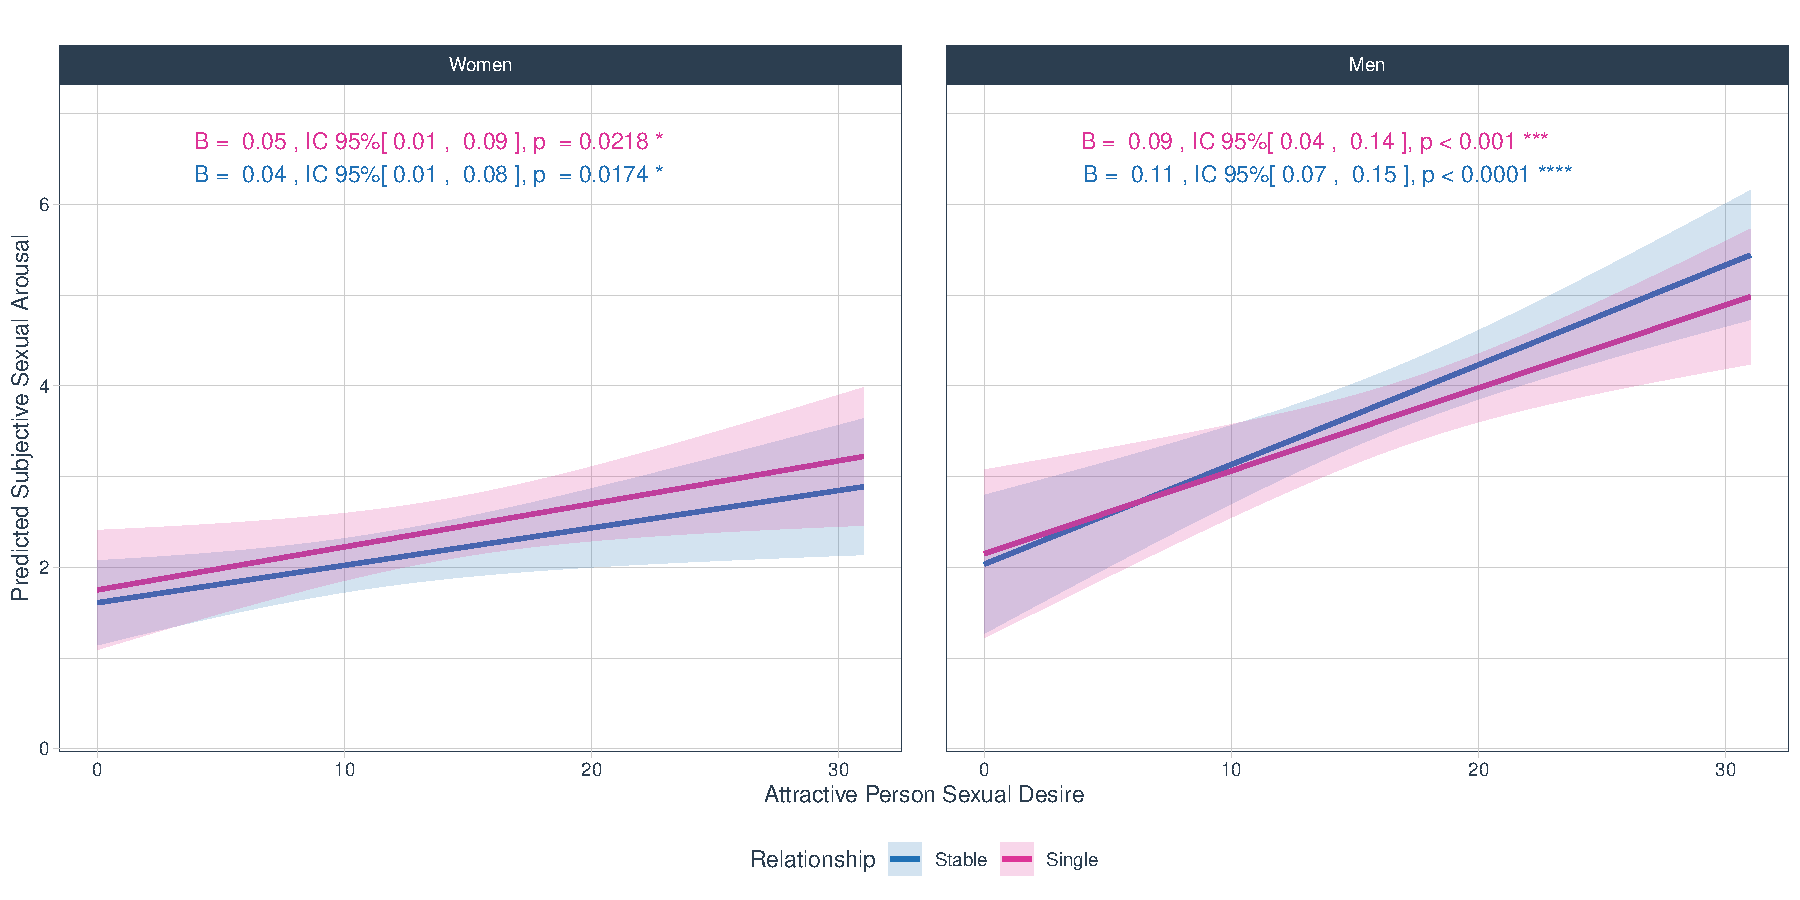
\includegraphics{Sexual_Desire_Arousal_anonymous_files/figure-latex/fig-h3b-1.pdf}
\caption{\label{fig:fig-h3b}Predicted subjective sexual arousal as a function of Dyadic TSD Partner, modeled using aLinear Mixed Model (LMM). Lines represent predicted values, and shaded areas indicate 95\% confidence intervals. The model include participant gender and relationship status as key factors.}
\end{figure}

\subsubsection{Hypothesis 3c: Dyadic TSD Partner}\label{hyp3c}

\paragraph{Model Robustness: Examining the Effects of Dyadic TSD Partner on SSA Across Gender and Stimuli Sex}\label{model-robustness-examining-the-effects-of-dyadic-tsd-partner-on-ssa-across-gender-and-stimuli-sex-1}

To assess the robustness of our findings, we fitted three different models examining how Dyadic TSD Partner predicts SSA, considering variations by gender and stimuli sex:

\begin{enumerate}
\def\labelenumi{\arabic{enumi}.}
\tightlist
\item
  Cumulative Link Mixed Model (CLMM) -- \texttt{m3c\_clmm} (for ordinal outcomes, using a probit link).
\item
  Generalized Linear Mixed Model (GLMM) with Poisson family -- \texttt{m3c\_poisson} (treating SSA as a count variable).
\item
  Linear Mixed Model (LMM) -- \texttt{m3c\_lmer} (treating SSA as a continuous variable).
\end{enumerate}

\begin{Shaded}
\begin{Highlighting}[]
\CommentTok{\# (1) Cumulative Link Mixed Model (CLMM) {-} Ordinal model with probit link}
\NormalTok{m3c\_clmm }\OtherTok{\textless{}{-}} \FunctionTok{clmm}\NormalTok{(}
\NormalTok{  Subjective.sexual.arousal.factor }\SpecialCharTok{\textasciitilde{}}\NormalTok{ Dyadic.TSD.Partner }\SpecialCharTok{*}\NormalTok{ Gender }\SpecialCharTok{*}\NormalTok{ Relationship }\SpecialCharTok{+}
\NormalTok{    (}\DecValTok{1} \SpecialCharTok{|}\NormalTok{ Stimuli.code) }\SpecialCharTok{+} \CommentTok{\# Random intercept to account for variance across stimuli}
\NormalTok{    (}\DecValTok{1} \SpecialCharTok{|}\NormalTok{ Participant), }\CommentTok{\# Random intercept \& slope for Relationship status}
  \AttributeTok{data =}\NormalTok{ dat\_m3,}
  \AttributeTok{link =} \StringTok{"probit"}\NormalTok{, }\CommentTok{\# Use a probit link function for ordinal outcomes}
  \AttributeTok{control =} \FunctionTok{list}\NormalTok{(}\AttributeTok{method =} \StringTok{"nlminb"}\NormalTok{) }\CommentTok{\# Use \textquotesingle{}nlminb\textquotesingle{} optimizer to improve convergence}
\NormalTok{)}

\CommentTok{\# (2) Generalized Linear Mixed Model (GLMM) {-} Poisson regression for count data}
\NormalTok{m3c\_poisson }\OtherTok{\textless{}{-}} \FunctionTok{glmer}\NormalTok{(}
\NormalTok{  Subjective.sexual.arousal }\SpecialCharTok{\textasciitilde{}}\NormalTok{ Dyadic.TSD.Partner }\SpecialCharTok{*}\NormalTok{ Gender }\SpecialCharTok{*}\NormalTok{ Relationship }\SpecialCharTok{+}
\NormalTok{    (}\DecValTok{1} \SpecialCharTok{|}\NormalTok{ Stimuli.code) }\SpecialCharTok{+} \CommentTok{\# Random intercept for Stimuli}
\NormalTok{    (}\DecValTok{1} \SpecialCharTok{|}\NormalTok{ Participant), }\CommentTok{\# Random intercept \& slope for Relationship status}
  \AttributeTok{data =}\NormalTok{ dat\_m3,}
  \AttributeTok{family =}\NormalTok{ poisson }\CommentTok{\# Use Poisson distribution for count{-}based SSA modeling}
\NormalTok{)}

\CommentTok{\# (3) Linear Mixed Model (LMM) {-} Continuous approximation}
\NormalTok{m3c\_lmer }\OtherTok{\textless{}{-}} \FunctionTok{lmer}\NormalTok{(}
\NormalTok{  Subjective.sexual.arousal }\SpecialCharTok{\textasciitilde{}}\NormalTok{ Dyadic.TSD.Partner }\SpecialCharTok{*}\NormalTok{ Gender }\SpecialCharTok{*}\NormalTok{ Relationship }\SpecialCharTok{+}
\NormalTok{    (}\DecValTok{1} \SpecialCharTok{|}\NormalTok{ Stimuli.code) }\SpecialCharTok{+} \CommentTok{\# Random intercept for Stimuli}
\NormalTok{    (}\DecValTok{1} \SpecialCharTok{|}\NormalTok{ Participant), }\CommentTok{\# Random intercept \& slope for Relationship status}
  \AttributeTok{data =}\NormalTok{ dat\_m3,}
  \AttributeTok{control =} \FunctionTok{lmerControl}\NormalTok{(}\AttributeTok{optimizer =} \StringTok{"bobyqa"}\NormalTok{) }\CommentTok{\# Use \textquotesingle{}bobyqa\textquotesingle{} optimizer for numerical stability}
\NormalTok{)}
\end{Highlighting}
\end{Shaded}

\subparagraph{Table \ref{tab:tab-robu-m3c}. ANOVA-type table of fixed effects (main effects and interactions) across the three fitted models}\label{table-reftabtab-robu-m3c.-anova-type-table-of-fixed-effects-main-effects-and-interactions-across-the-three-fitted-models}

As shown in the table below, the pattern of significant effects remains consistent across all three models, except for the main effect of gender, which is not significant in the CLMM.

\begin{Shaded}
\begin{Highlighting}[]
\CommentTok{\# Generate an ANOVA{-}type comparison table for fixed effects across the three models}
\FunctionTok{anova.comp}\NormalTok{(}
  \AttributeTok{CLMMmod =}\NormalTok{ m3c\_clmm, }\CommentTok{\# Cumulative Link Mixed Model (CLMM) {-} ordinal outcome}
  \AttributeTok{GLMERmod =}\NormalTok{ m3c\_poisson, }\CommentTok{\# Generalized Linear Mixed Model (GLMM) {-} Poisson outcome}
  \AttributeTok{LMERmod =}\NormalTok{ m3c\_lmer, }\CommentTok{\# Linear Mixed Model (LMM) {-} continuous outcome}
  \AttributeTok{hypothesis =} \StringTok{"3c"} \CommentTok{\# Specify hypothesis being tested}
\NormalTok{)}
\end{Highlighting}
\end{Shaded}

\begin{table}[H]
\centering
\caption{\label{tab:tab-robu-m3c}Comparison of fixed effects across the three models for Hypothesis 3c: CLMM, GLMM (Poisson), and LMM.}
\centering
\resizebox{\ifdim\width>\linewidth\linewidth\else\width\fi}{!}{
\begin{threeparttable}
\begin{tabular}[t]{lccccccccc}
\toprule
\multicolumn{1}{c}{ } & \multicolumn{3}{c}{CLMM} & \multicolumn{3}{c}{GLMER (Poisson)} & \multicolumn{3}{c}{LMM} \\
\cmidrule(l{3pt}r{3pt}){2-4} \cmidrule(l{3pt}r{3pt}){5-7} \cmidrule(l{3pt}r{3pt}){8-10}
Effect & $df$ & $\chi^2$ & $p$ & $df$ & $\chi^2$ & $p$ & $df$ & $F$ & $p$\\
\midrule
Dyadic TSD Partner & 1 & 0.039 & 0.84 & 1 & 2.932 & 0.09 & 1, 311.9 & 3.163 & 0.08\\
Gender & 1 & 2.276 & 0.13 & 1 & 2.719 & 0.1 & 1, 328.45 & 2.500 & 0.11\\
Relationship & 1 & 0.080 & 0.78 & 1 & 0.062 & 0.8 & 1, 311.9 & 0.670 & 0.41\\
Dyadic TSD Partner × Gender & 1 & 0.645 & 0.42 & 1 & 0.651 & 0.42 & 1, 311.98 & 1.153 & 0.28\\
Dyadic TSD Partner × Relationship & 1 & 0.471 & 0.49 & 1 & 0.501 & 0.48 & 1, 311.9 & 1.374 & 0.24\\
Gender × Relationship & 1 & 4.340 & \textbf{0.0372} & 1 & 7.102 & \textbf{0.0077} & 1, 311.9 & 8.505 & \textbf{0.0038}\\
Dyadic TSD Partner × Gender × Relationship & 1 & 3.905 & \textbf{0.0481} & 1 & 6.593 & \textbf{0.0102} & 1, 311.94 & 8.308 & \textbf{0.0042}\\
\bottomrule
\end{tabular}
\begin{tablenotes}[para]
\item \textit{Note: } 
\item For CLMM and GLMER (Poisson) models, results are
              Analysis of Deviance (Type III Wald chi-square tests),
              while for LMM, results are from an Analysis of Variance
              (Type III ANOVA with Satterthwaite's method).
              Significant effects are in bold.
\end{tablenotes}
\end{threeparttable}}
\end{table}

\subparagraph{Figure \ref{fig:preds-m3c}: Model-based predictions for Hypothesis 3c.}\label{figure-reffigpreds-m3c-model-based-predictions-for-hypothesis-3c.}

This figure presents model-based predictions of subjective sexual arousal as a function of Dyadic TSD Partner, across different relationship status and participant genders. The three subplots correspond to the three statistical models used for analysis: (a) Cumulative Link Mixed Model (CLMM), (b) Generalized Linear Mixed Model (GLMM, Poisson), and (c) Linear Mixed Model (LMM). Shaded areas represent 95\% confidence intervals.

\begin{Shaded}
\begin{Highlighting}[]
\CommentTok{\# CLMM Predictions}
\NormalTok{p\_m3c\_clmm }\OtherTok{\textless{}{-}} \FunctionTok{emmeans}\NormalTok{(m3c\_clmm, }\SpecialCharTok{\textasciitilde{}}\NormalTok{ Dyadic.TSD.Partner }\SpecialCharTok{|}\NormalTok{ Gender }\SpecialCharTok{*}\NormalTok{ Relationship,}
  \AttributeTok{at =} \FunctionTok{list}\NormalTok{(}\AttributeTok{Dyadic.TSD.Partner =} \FunctionTok{seq}\NormalTok{(}\DecValTok{0}\NormalTok{, }\DecValTok{31}\NormalTok{, }\AttributeTok{length.out =} \DecValTok{100}\NormalTok{)), }\CommentTok{\# Generate 100 points}
  \AttributeTok{mode =} \StringTok{"mean.class"} \CommentTok{\# Compute predicted mean response categories}
\NormalTok{) }\SpecialCharTok{|\textgreater{}}
  \FunctionTok{as.data.frame}\NormalTok{() }\SpecialCharTok{|\textgreater{}} \CommentTok{\# Convert predictions to a dataframe}
  \FunctionTok{ggplot}\NormalTok{(}\FunctionTok{aes}\NormalTok{(}
    \AttributeTok{x =}\NormalTok{ Dyadic.TSD.Partner, }\AttributeTok{y =}\NormalTok{ mean.class,}
    \AttributeTok{color =}\NormalTok{ Relationship, }\AttributeTok{fill =}\NormalTok{ Relationship}
\NormalTok{  )) }\SpecialCharTok{+}
  \FunctionTok{geom\_line}\NormalTok{(}\AttributeTok{size =} \DecValTok{1}\NormalTok{) }\SpecialCharTok{+} \CommentTok{\# Add predicted response line}
  \FunctionTok{geom\_ribbon}\NormalTok{(}\FunctionTok{aes}\NormalTok{(}\AttributeTok{ymin =}\NormalTok{ asymp.LCL, }\AttributeTok{ymax =}\NormalTok{ asymp.UCL, }\AttributeTok{fill =}\NormalTok{ Relationship),}
    \AttributeTok{alpha =} \FloatTok{0.2}\NormalTok{, }\AttributeTok{color =} \ConstantTok{NA}
\NormalTok{  ) }\SpecialCharTok{+} \CommentTok{\# Add confidence interval}
  \FunctionTok{scale\_color\_manual}\NormalTok{(}\AttributeTok{values =}\NormalTok{ color.Relationship) }\SpecialCharTok{+} \CommentTok{\# Apply custom colors}
  \FunctionTok{scale\_fill\_manual}\NormalTok{(}\AttributeTok{values =}\NormalTok{ color.Relationship) }\SpecialCharTok{+}
  \FunctionTok{facet\_wrap}\NormalTok{(}\SpecialCharTok{\textasciitilde{}}\NormalTok{Gender, }\AttributeTok{ncol =} \DecValTok{1}\NormalTok{) }\SpecialCharTok{+} \CommentTok{\# Separate plots by gender}
  \FunctionTok{labs}\NormalTok{(}
    \AttributeTok{y =} \StringTok{"Predicted Subjective Sexual Arousal"}\NormalTok{, }\AttributeTok{x =} \StringTok{"Dyadic TSD Partner"}\NormalTok{,}
    \AttributeTok{title =} \StringTok{"CLMM"}
\NormalTok{  ) }\SpecialCharTok{+}
  \FunctionTok{theme\_tq}\NormalTok{() }\SpecialCharTok{+} \CommentTok{\# Apply theme}
  \FunctionTok{theme}\NormalTok{(}\AttributeTok{legend.position =} \StringTok{"bottom"}\NormalTok{) }\SpecialCharTok{+}
  \FunctionTok{ylim}\NormalTok{(}\FunctionTok{c}\NormalTok{(}\FloatTok{0.3}\NormalTok{, }\DecValTok{8}\NormalTok{)) }\CommentTok{\# Set Y{-}axis limits}

\CommentTok{\# Poisson GLMM Predictions}
\NormalTok{p\_m3c\_poisson }\OtherTok{\textless{}{-}} \FunctionTok{emmeans}\NormalTok{(m3c\_poisson, }\SpecialCharTok{\textasciitilde{}}\NormalTok{ Dyadic.TSD.Partner }\SpecialCharTok{|}\NormalTok{ Gender }\SpecialCharTok{*}\NormalTok{ Relationship,}
  \AttributeTok{at =} \FunctionTok{list}\NormalTok{(}\AttributeTok{Dyadic.TSD.Partner =} \FunctionTok{seq}\NormalTok{(}\DecValTok{0}\NormalTok{, }\DecValTok{31}\NormalTok{, }\AttributeTok{length.out =} \DecValTok{100}\NormalTok{)), }\CommentTok{\# Generate 100 points}
  \AttributeTok{type =} \StringTok{"response"} \CommentTok{\# Compute response{-}scale predictions}
\NormalTok{) }\SpecialCharTok{|\textgreater{}}
  \FunctionTok{as.data.frame}\NormalTok{() }\SpecialCharTok{|\textgreater{}}
  \FunctionTok{ggplot}\NormalTok{(}\FunctionTok{aes}\NormalTok{(}
    \AttributeTok{x =}\NormalTok{ Dyadic.TSD.Partner, }\AttributeTok{y =}\NormalTok{ rate,}
    \AttributeTok{color =}\NormalTok{ Relationship, }\AttributeTok{fill =}\NormalTok{ Relationship}
\NormalTok{  )) }\SpecialCharTok{+}
  \FunctionTok{geom\_line}\NormalTok{(}\AttributeTok{size =} \DecValTok{1}\NormalTok{) }\SpecialCharTok{+}
  \FunctionTok{geom\_ribbon}\NormalTok{(}\FunctionTok{aes}\NormalTok{(}\AttributeTok{ymin =}\NormalTok{ asymp.LCL, }\AttributeTok{ymax =}\NormalTok{ asymp.UCL, }\AttributeTok{fill =}\NormalTok{ Relationship),}
    \AttributeTok{alpha =} \FloatTok{0.2}\NormalTok{, }\AttributeTok{color =} \ConstantTok{NA}
\NormalTok{  ) }\SpecialCharTok{+}
  \FunctionTok{scale\_color\_manual}\NormalTok{(}\AttributeTok{values =}\NormalTok{ color.Relationship) }\SpecialCharTok{+}
  \FunctionTok{scale\_fill\_manual}\NormalTok{(}\AttributeTok{values =}\NormalTok{ color.Relationship) }\SpecialCharTok{+}
  \FunctionTok{facet\_wrap}\NormalTok{(}\SpecialCharTok{\textasciitilde{}}\NormalTok{Gender, }\AttributeTok{ncol =} \DecValTok{1}\NormalTok{) }\SpecialCharTok{+}
  \FunctionTok{labs}\NormalTok{(}\AttributeTok{y =} \StringTok{""}\NormalTok{, }\AttributeTok{x =} \StringTok{"Dyadic TSD Partner"}\NormalTok{, }\AttributeTok{title =} \StringTok{"GLMER (Poisson)"}\NormalTok{) }\SpecialCharTok{+}
  \FunctionTok{theme\_tq}\NormalTok{() }\SpecialCharTok{+}
  \FunctionTok{theme}\NormalTok{(}\AttributeTok{legend.position =} \StringTok{"bottom"}\NormalTok{) }\SpecialCharTok{+}
  \FunctionTok{ylim}\NormalTok{(}\FunctionTok{c}\NormalTok{(}\FloatTok{0.3}\NormalTok{, }\DecValTok{8}\NormalTok{))}

\CommentTok{\# LMM Predictions}
\NormalTok{p\_m3c\_lmer }\OtherTok{\textless{}{-}} \FunctionTok{emmeans}\NormalTok{(m3c\_lmer, }\SpecialCharTok{\textasciitilde{}}\NormalTok{ Dyadic.TSD.Partner }\SpecialCharTok{|}\NormalTok{ Gender }\SpecialCharTok{*}\NormalTok{ Relationship,}
  \AttributeTok{at =} \FunctionTok{list}\NormalTok{(}\AttributeTok{Dyadic.TSD.Partner =} \FunctionTok{seq}\NormalTok{(}\DecValTok{0}\NormalTok{, }\DecValTok{31}\NormalTok{, }\AttributeTok{length.out =} \DecValTok{100}\NormalTok{)),}
  \AttributeTok{type =} \StringTok{"response"}
\NormalTok{) }\SpecialCharTok{|\textgreater{}}
  \FunctionTok{as.data.frame}\NormalTok{() }\SpecialCharTok{|\textgreater{}}
  \FunctionTok{ggplot}\NormalTok{(}\FunctionTok{aes}\NormalTok{(}
    \AttributeTok{x =}\NormalTok{ Dyadic.TSD.Partner, }\AttributeTok{y =}\NormalTok{ emmean,}
    \AttributeTok{color =}\NormalTok{ Relationship, }\AttributeTok{fill =}\NormalTok{ Relationship}
\NormalTok{  )) }\SpecialCharTok{+}
  \FunctionTok{geom\_line}\NormalTok{(}\AttributeTok{size =} \DecValTok{1}\NormalTok{) }\SpecialCharTok{+}
  \FunctionTok{geom\_ribbon}\NormalTok{(}\FunctionTok{aes}\NormalTok{(}\AttributeTok{ymin =}\NormalTok{ asymp.LCL, }\AttributeTok{ymax =}\NormalTok{ asymp.UCL, }\AttributeTok{fill =}\NormalTok{ Relationship),}
    \AttributeTok{alpha =} \FloatTok{0.2}\NormalTok{, }\AttributeTok{color =} \ConstantTok{NA}
\NormalTok{  ) }\SpecialCharTok{+}
  \FunctionTok{scale\_color\_manual}\NormalTok{(}\AttributeTok{values =}\NormalTok{ color.Relationship) }\SpecialCharTok{+}
  \FunctionTok{scale\_fill\_manual}\NormalTok{(}\AttributeTok{values =}\NormalTok{ color.Relationship) }\SpecialCharTok{+}
  \FunctionTok{facet\_wrap}\NormalTok{(}\SpecialCharTok{\textasciitilde{}}\NormalTok{Gender, }\AttributeTok{ncol =} \DecValTok{1}\NormalTok{) }\SpecialCharTok{+}
  \FunctionTok{labs}\NormalTok{(}\AttributeTok{y =} \StringTok{""}\NormalTok{, }\AttributeTok{x =} \StringTok{"Dyadic TSD Partner"}\NormalTok{, }\AttributeTok{title =} \StringTok{"LMM"}\NormalTok{) }\SpecialCharTok{+}
  \FunctionTok{theme\_tq}\NormalTok{() }\SpecialCharTok{+}
  \FunctionTok{theme}\NormalTok{(}\AttributeTok{legend.position =} \StringTok{"bottom"}\NormalTok{) }\SpecialCharTok{+}
  \FunctionTok{ylim}\NormalTok{(}\FunctionTok{c}\NormalTok{(}\FloatTok{0.3}\NormalTok{, }\DecValTok{8}\NormalTok{))}

\CommentTok{\# Arrange Plots into a Single Figure}
\NormalTok{p\_robu\_m3c }\OtherTok{\textless{}{-}} \FunctionTok{ggarrange}\NormalTok{(p\_m3c\_clmm, p\_m3c\_poisson, p\_m3c\_lmer, }\CommentTok{\# Combine plots side by side}
  \AttributeTok{common.legend =} \ConstantTok{TRUE}\NormalTok{, }\CommentTok{\# Share legend across plots}
  \AttributeTok{labels =} \StringTok{"auto"}\NormalTok{, }\CommentTok{\# Automatically label subfigures (a, b, c)}
  \AttributeTok{legend =} \StringTok{"bottom"}\NormalTok{,}
  \AttributeTok{nrow =} \DecValTok{1} \CommentTok{\# Arrange in a single row}
\NormalTok{)}

\CommentTok{\# Display the combined figure}
\NormalTok{p\_robu\_m3c}
\end{Highlighting}
\end{Shaded}

\begin{figure}
\centering
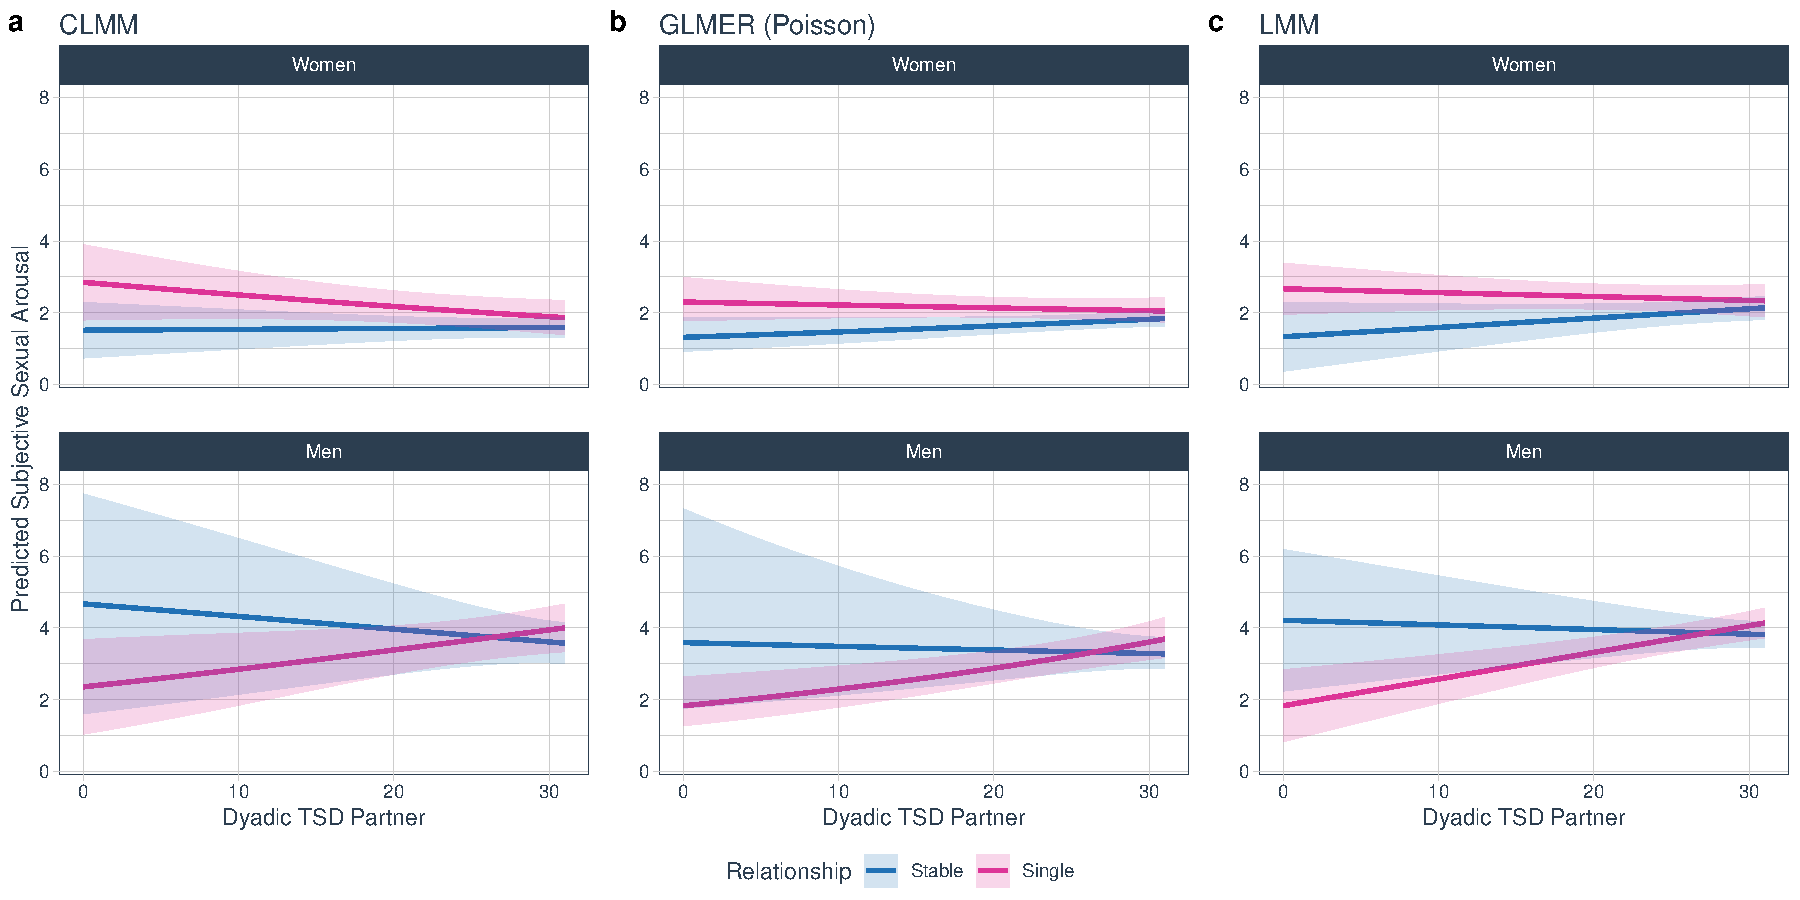
\includegraphics{Sexual_Desire_Arousal_anonymous_files/figure-latex/preds-m3c-1.pdf}
\caption{\label{fig:preds-m3c}Predicted subjective sexual arousal as a function of Dyadic TSD Partner, modeled using three statistical approaches: \textbf{(a)} Cumulative Link Mixed Model (CLMM); \textbf{(b)} Generalized Linear Mixed Model (GLMM) with a Poisson family; \textbf{(c)} Linear Mixed Model (LMM). Lines represent predicted values, and shaded areas indicate 95\% confidence intervals. The models include participant gender and relationship status as key factors.}
\end{figure}

\paragraph{Final Model: Effects of Dyadic TSD Partner on SSA Across Gender and Stimuli Sex}\label{final-model-effects-of-dyadic-tsd-partner-on-ssa-across-gender-and-stimuli-sex-1}

Given the apparent robustness of most results across models (CLMM, GLMER and LMM; Table \ref{tab:tab-robu-m3c}, Fig. \ref{fig:preds-m3c}), we test the predictions of the hypothesis from the LMM (\texttt{m3c\_lmer}).

\subparagraph{\texorpdfstring{Table \ref{tab:tab-m3c}. ANOVA-type table for the interaction between \texttt{Relationship\ type}, and \texttt{Gender}}{Table \ref{tab:tab-m3c}. ANOVA-type table for the interaction between Relationship type, and Gender}}\label{table-reftabtab-m3c.-anova-type-table-for-the-interaction-between-relationship-type-and-gender}

This tables summarizes the results of the model.

\begin{Shaded}
\begin{Highlighting}[]
\CommentTok{\# Generate ANOVA{-}type table for the final LMM model}
\CommentTok{\# This summarizes the effects of Dyadic TSD Partner on SSA across Gender and Stimuli Sex}
\FunctionTok{anova.sig.lmer}\NormalTok{(}
  \AttributeTok{model =}\NormalTok{ m3c\_lmer, }\CommentTok{\# Use LMM as the final model}
  \AttributeTok{custom\_caption =} \StringTok{"Effects of Dyadic TSD Partner on SSA Across Gender and Stimuli Sex"}
\NormalTok{)}
\end{Highlighting}
\end{Shaded}

\begin{table}[H]
\centering
\caption{\label{tab:tab-m3c}Effects of Dyadic TSD Partner on SSA Across Gender and Stimuli Sex}
\centering
\resizebox{\ifdim\width>\linewidth\linewidth\else\width\fi}{!}{
\begin{threeparttable}
\begin{tabular}[t]{lcccc}
\toprule
Effect & $df$ & $F$ & $p$ & $\epsilon^2_p$\\
\midrule
Dyadic TSD Partner & 1, 311.9 & 3.16 & 0.08 & 0.0069\\
Gender & 1, 328.45 & 2.50 & 0.11 & 0.0045\\
Relationship & 1, 311.9 & 0.67 & 0.41 & < 0.0001\\
Dyadic TSD Partner × Gender & 1, 311.98 & 1.15 & 0.28 & < 0.001\\
Dyadic TSD Partner × Relationship & 1, 311.9 & 1.37 & 0.24 & 0.0012\\
Gender × Relationship & 1, 311.9 & 8.51 & \textbf{0.0038} & 0.0234\\
Dyadic TSD Partner × Gender × Relationship & 1, 311.94 & 8.31 & \textbf{0.0042} & 0.0228\\
\bottomrule
\end{tabular}
\begin{tablenotes}[para]
\item \textit{Note: } 
\item Results are Type III ANOVA. $R^2_{conditional}$ = 0.719, $R^2_{marginal}$ = 0.182. As effect size, we report partial epsilon squared ($\epsilon^2_p$), a less biased estimate than $\eta^2$ (see \cite{albersWhenPowerAnalyses2018}). Significant effects are in bold.
\end{tablenotes}
\end{threeparttable}}
\end{table}

\subparagraph{\texorpdfstring{\emph{Post-hoc} tests}{Post-hoc tests}}\label{post-hoc-tests-5}

To test the hypothesis, which predicted that there would be different relationship between SSA and Dyadic TSD Partner, and that this association differ between men and women depending on the sex of stimuli, we used simple slope analysis.

\begin{Shaded}
\begin{Highlighting}[]
\CommentTok{\# Perform simple slope analysis to examine how Dyadic TSD Partner predicts SSA}
\CommentTok{\# The model includes relationship status and gender as moderators}
\NormalTok{slop.m3c\_lmer }\OtherTok{\textless{}{-}} \FunctionTok{sim\_slopes}\NormalTok{(}
\NormalTok{  m3c\_lmer,}
  \AttributeTok{pred =}\NormalTok{ Dyadic.TSD.Partner, }\CommentTok{\# Predictor: Dyadic TSD Partner}
  \AttributeTok{modx =}\NormalTok{ Relationship, }\CommentTok{\# First moderator: Relationship status}
  \AttributeTok{mod2 =}\NormalTok{ Gender, }\CommentTok{\# Second moderator: Gender}
  \AttributeTok{confint =} \ConstantTok{TRUE} \CommentTok{\# Compute confidence intervals}
\NormalTok{)}

\CommentTok{\# Bind slopes for women and men into a single table, adding Gender as a column}
\NormalTok{slop.m3c\_lmer.tab }\OtherTok{\textless{}{-}} \FunctionTok{bind\_rows}\NormalTok{(}
\NormalTok{  slop.m3c\_lmer}\SpecialCharTok{$}\NormalTok{slopes[[}\DecValTok{1}\NormalTok{]] }\SpecialCharTok{|\textgreater{}} \FunctionTok{mutate}\NormalTok{(}\AttributeTok{Gender =} \StringTok{"Women"}\NormalTok{),}
\NormalTok{  slop.m3c\_lmer}\SpecialCharTok{$}\NormalTok{slopes[[}\DecValTok{2}\NormalTok{]] }\SpecialCharTok{|\textgreater{}} \FunctionTok{mutate}\NormalTok{(}\AttributeTok{Gender =} \StringTok{"Men"}\NormalTok{)}
\NormalTok{) }\SpecialCharTok{|\textgreater{}}
  \CommentTok{\# Recode Gender variable to English labels}
  \FunctionTok{mutate}\NormalTok{(}\AttributeTok{Gender =} \FunctionTok{recode\_factor}\NormalTok{(Gender, }\AttributeTok{Femenino =} \StringTok{"Women"}\NormalTok{, }\AttributeTok{Masculino =} \StringTok{"Men"}\NormalTok{)) }\SpecialCharTok{|\textgreater{}}
  \CommentTok{\# Select relevant columns (reordering for clarity)}
  \FunctionTok{select}\NormalTok{(}\DecValTok{8}\NormalTok{, }\DecValTok{1}\SpecialCharTok{:}\DecValTok{2}\NormalTok{, }\DecValTok{4}\SpecialCharTok{:}\DecValTok{7}\NormalTok{) }\SpecialCharTok{|\textgreater{}}
  \CommentTok{\# Convert specific columns to numeric format}
  \FunctionTok{mutate}\NormalTok{(}\FunctionTok{across}\NormalTok{(}\DecValTok{3}\SpecialCharTok{:}\DecValTok{7}\NormalTok{, as.numeric)) }\SpecialCharTok{|\textgreater{}}
  \CommentTok{\# Round coefficients and confidence intervals to 2 decimal places}
  \FunctionTok{mutate}\NormalTok{(}\FunctionTok{across}\NormalTok{(}\DecValTok{3}\SpecialCharTok{:}\DecValTok{6}\NormalTok{, round, }\DecValTok{2}\NormalTok{)) }\SpecialCharTok{|\textgreater{}}
  \CommentTok{\# Add significance stars based on p{-}values}
  \FunctionTok{mutate}\NormalTok{(}\AttributeTok{sig =} \FunctionTok{pval.stars}\NormalTok{(p)) }\SpecialCharTok{|\textgreater{}}
  \CommentTok{\# Rename columns for clarity}
  \FunctionTok{rename}\NormalTok{(}\StringTok{"Relationship"} \OtherTok{=} \StringTok{"Value of Relationship"}\NormalTok{) }\SpecialCharTok{|\textgreater{}}
  \FunctionTok{rename}\NormalTok{(}\AttributeTok{Coefficient =}\NormalTok{ Est.)}

\CommentTok{\# Create formatted output table}
\NormalTok{slop.m3c\_lmer.tab[, }\SpecialCharTok{{-}}\FunctionTok{c}\NormalTok{(}\DecValTok{1}\NormalTok{, }\DecValTok{8}\NormalTok{)] }\SpecialCharTok{|\textgreater{}} \CommentTok{\# Exclude unnecessary columns}
  \FunctionTok{mutate}\NormalTok{(}\AttributeTok{p =} \FunctionTok{pval.lev}\NormalTok{(p)) }\SpecialCharTok{|\textgreater{}} \CommentTok{\# Format p{-}values}
  \FunctionTok{kable}\NormalTok{(}
    \AttributeTok{booktabs =} \ConstantTok{TRUE}\NormalTok{,}
    \AttributeTok{align =} \FunctionTok{c}\NormalTok{(}\StringTok{"l"}\NormalTok{, }\FunctionTok{rep}\NormalTok{(}\StringTok{"c"}\NormalTok{, }\DecValTok{5}\NormalTok{)), }\CommentTok{\# Align columns}
    \AttributeTok{caption =} \StringTok{"Slope for Dyadic TSD Partner on Subjective sexual arousal}
\StringTok{               by stimuli sex and gender"}\NormalTok{,}
    \AttributeTok{linesep =} \StringTok{""}\NormalTok{,}
    \AttributeTok{col.names =} \FunctionTok{c}\NormalTok{(}\StringTok{"Relationship status"}\NormalTok{, }\StringTok{"$B$"}\NormalTok{, }\StringTok{"$2.5}\SpecialCharTok{\textbackslash{}\textbackslash{}}\StringTok{\% CI$"}\NormalTok{, }\StringTok{"$97.5}\SpecialCharTok{\textbackslash{}\textbackslash{}}\StringTok{\% CI$"}\NormalTok{, }\StringTok{"$t$"}\NormalTok{, }\StringTok{"$p$"}\NormalTok{),}
    \AttributeTok{escape =} \ConstantTok{FALSE}
\NormalTok{  ) }\SpecialCharTok{|\textgreater{}}
  \CommentTok{\# Apply table styling}
  \FunctionTok{kable\_styling}\NormalTok{(}\AttributeTok{latex\_options =} \FunctionTok{c}\NormalTok{(}\StringTok{"HOLD\_position"}\NormalTok{)) }\SpecialCharTok{|\textgreater{}}
  \CommentTok{\# Group rows by gender for better readability}
  \FunctionTok{pack\_rows}\NormalTok{(}\StringTok{"Gender: Women"}\NormalTok{, }\AttributeTok{start\_row =} \DecValTok{1}\NormalTok{, }\AttributeTok{end\_row =} \DecValTok{2}\NormalTok{, }
            \AttributeTok{bold =} \ConstantTok{FALSE}\NormalTok{, }\AttributeTok{background =} \StringTok{"lightgray"}\NormalTok{) }\SpecialCharTok{|\textgreater{}}
  \FunctionTok{pack\_rows}\NormalTok{(}\StringTok{"Gender: Men"}\NormalTok{, }\AttributeTok{start\_row =} \DecValTok{3}\NormalTok{, }\AttributeTok{end\_row =} \DecValTok{4}\NormalTok{, }
            \AttributeTok{bold =} \ConstantTok{FALSE}\NormalTok{, }\AttributeTok{background =} \StringTok{"lightgray"}\NormalTok{) }\SpecialCharTok{|\textgreater{}}
  \CommentTok{\# Add a footnote for coefficient interpretation}
  \FunctionTok{footnote}\NormalTok{(}
    \AttributeTok{general =} \StringTok{"$B$ are unstandardized coefficients. No intercept is reported}
\StringTok{               as continuous predictors were centered and are dependent on this sample."}\NormalTok{,}
    \AttributeTok{threeparttable =} \ConstantTok{TRUE}\NormalTok{,}
    \AttributeTok{footnote\_as\_chunk =} \ConstantTok{TRUE}\NormalTok{,}
    \AttributeTok{escape =} \ConstantTok{FALSE}
\NormalTok{  )}
\end{Highlighting}
\end{Shaded}

\begin{table}[H]
\centering
\caption{\label{tab:unnamed-chunk-32}Slope for Dyadic TSD Partner on Subjective sexual arousal
               by stimuli sex and gender}
\centering
\begin{threeparttable}
\begin{tabular}[t]{lccccc}
\toprule
Relationship status & $B$ & $2.5\% CI$ & $97.5\% CI$ & $t$ & $p$\\
\midrule
\addlinespace[0.3em]
\multicolumn{6}{l}{\cellcolor{lightgray}{Gender: Women}}\\
\hspace{1em}Stable & 0.03 & -0.01 & 0.06 & 1.54 & 0.12\\
\hspace{1em}Single & -0.01 & -0.04 & 0.02 & -0.73 & 0.47\\
\addlinespace[0.3em]
\multicolumn{6}{l}{\cellcolor{lightgray}{Gender: Men}}\\
\hspace{1em}Stable & -0.01 & -0.07 & 0.05 & -0.41 & 0.68\\
\hspace{1em}Single & 0.07 & 0.04 & 0.11 & 4.02 & \textbf{< 0.0001}\\
\bottomrule
\end{tabular}
\begin{tablenotes}[para]
\item \textit{Note: } 
\item $B$ are unstandardized coefficients. No intercept is reported
               as continuous predictors were centered and are dependent on this sample.
\end{tablenotes}
\end{threeparttable}
\end{table}

\paragraph{Figure \ref{fig:fig-h3c}. Subjective sexual arousal to erotic stimuli: Main effects and interactions}\label{figure-reffigfig-h3c.-subjective-sexual-arousal-to-erotic-stimuli-main-effects-and-interactions}

This figure summarizes the results of hypothesis 3c.

\begin{Shaded}
\begin{Highlighting}[]
\CommentTok{\# Generate figure to visualize interaction between Relationship status and Gender}
\NormalTok{p\_m3c.fin }\OtherTok{\textless{}{-}}\NormalTok{ p\_m3c\_lmer }\SpecialCharTok{+}
  \CommentTok{\# Set axis labels (removing title for a cleaner look)}
  \FunctionTok{labs}\NormalTok{(}\AttributeTok{title =} \StringTok{""}\NormalTok{, }\AttributeTok{y =} \StringTok{"Predicted Subjective Sexual Arousal"}\NormalTok{) }\SpecialCharTok{+}
  \CommentTok{\# Facet by Gender, displaying two columns}
  \FunctionTok{facet\_wrap}\NormalTok{(}\SpecialCharTok{\textasciitilde{}}\NormalTok{Gender, }\AttributeTok{ncol =} \DecValTok{2}\NormalTok{) }\SpecialCharTok{+}
  \CommentTok{\# Add text labels for regression slopes}
  \FunctionTok{geom\_text}\NormalTok{(}
    \AttributeTok{data =}\NormalTok{ slop.m3c\_lmer.tab }\SpecialCharTok{|\textgreater{}} \FunctionTok{mutate}\NormalTok{(}\AttributeTok{Dyadic.TSD.Partner =} \DecValTok{2}\NormalTok{),}
    \AttributeTok{mapping =} \FunctionTok{aes}\NormalTok{(}
      \AttributeTok{x =} \FunctionTok{min}\NormalTok{(Dyadic.TSD.Partner), }\AttributeTok{y =} \ConstantTok{Inf}\NormalTok{,}
      \AttributeTok{label =} \FunctionTok{paste}\NormalTok{(}
        \StringTok{"B = "}\NormalTok{, Coefficient, }\StringTok{", IC 95\%["}\NormalTok{, }\StringTok{\textasciigrave{}}\AttributeTok{2.5\%}\StringTok{\textasciigrave{}}\NormalTok{, }\StringTok{", "}\NormalTok{, }\StringTok{\textasciigrave{}}\AttributeTok{97.5\%}\StringTok{\textasciigrave{}}\NormalTok{, }\StringTok{"], p"}\NormalTok{,}
        \FunctionTok{ifelse}\NormalTok{(}
          \FunctionTok{grepl}\NormalTok{(}\StringTok{"\textless{}"}\NormalTok{, }\FunctionTok{pe2.lev}\NormalTok{(p)), }\FunctionTok{pe2.lev}\NormalTok{(p), }\FunctionTok{paste0}\NormalTok{(}\StringTok{" = "}\NormalTok{, }\FunctionTok{pe2.lev}\NormalTok{(p))}
\NormalTok{        ),}
        \FunctionTok{ifelse}\NormalTok{(}\FunctionTok{is.na}\NormalTok{(sig), }\StringTok{""}\NormalTok{, sig) }\CommentTok{\# Add significance stars if applicable}
\NormalTok{      ),}
      \AttributeTok{vjust =} \DecValTok{2} \SpecialCharTok{+} \FunctionTok{as.numeric}\NormalTok{(}\FunctionTok{as.factor}\NormalTok{(Relationship)) }\SpecialCharTok{*} \DecValTok{2} \CommentTok{\# Adjust vertical spacing}
\NormalTok{    ),}
    \AttributeTok{hjust =} \SpecialCharTok{{-}}\FloatTok{0.1}\NormalTok{, }\CommentTok{\# Align text slightly to the left}
    \CommentTok{\# size = 3,  \# Uncomment to control text size if needed}
    \AttributeTok{show.legend =} \ConstantTok{FALSE} \CommentTok{\# Hide legend for text labels}
\NormalTok{  ) }\SpecialCharTok{+}
  \CommentTok{\# Move legend to the bottom}
  \FunctionTok{theme}\NormalTok{(}\AttributeTok{legend.position =} \StringTok{"bottom"}\NormalTok{)}

\CommentTok{\# Display the final plot}
\NormalTok{p\_m3c.fin}
\end{Highlighting}
\end{Shaded}

\begin{figure}
\centering
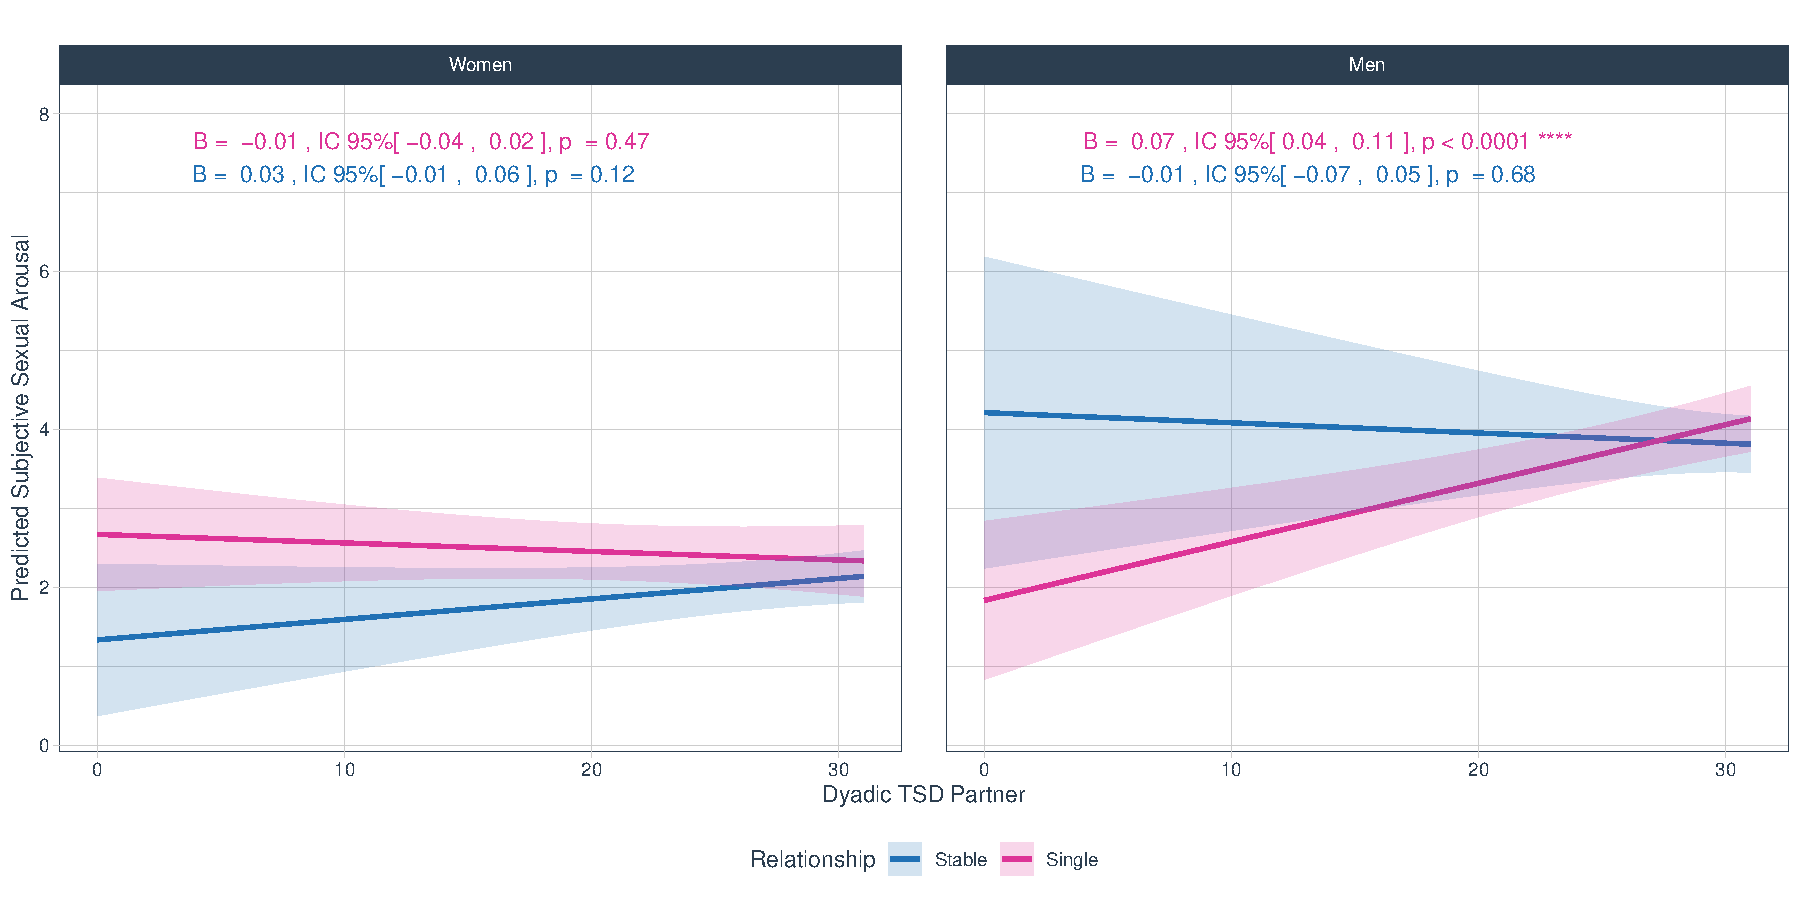
\includegraphics{Sexual_Desire_Arousal_anonymous_files/figure-latex/fig-h3c-1.pdf}
\caption{\label{fig:fig-h3c}Predicted subjective sexual arousal as a function of Dyadic TSD Partner, modeled using aLinear Mixed Model (LMM). Lines represent predicted values, and shaded areas indicate 95\% confidence intervals. The model include participant gender and relationship status as key factors.}
\end{figure}

\begin{center}\rule{0.5\linewidth}{0.5pt}\end{center}

\closesupplement

\section{Final figures and tables}\label{final-figures-and-tables}

Figures and tables included in the main document.

\subsection{Table \ref{tab:tab-m1-fin}. Hypothesis 1}\label{table-reftabtab-m1-fin.-hypothesis-1}

ANOVA-type table for the interaction between \texttt{Relationship\ type}, and \texttt{Gender} for the three final models for hypothesis 1.

\begin{Shaded}
\begin{Highlighting}[]
\CommentTok{\# Generate ANOVA{-}type table for the interaction between Relationship type and Gender}
\CommentTok{\# across the three final models for Hypothesis 1}
\FunctionTok{reduce}\NormalTok{(}
  \FunctionTok{list}\NormalTok{(}
    \CommentTok{\# Compute ANOVA summary for Solitary TSD}
    \FunctionTok{bind\_cols}\NormalTok{(}
      \FunctionTok{anova\_summary}\NormalTok{(}\FunctionTok{Anova}\NormalTok{(m1a\_norm, }\AttributeTok{type =} \DecValTok{3}\NormalTok{)),}
      \FunctionTok{epsilon\_squared}\NormalTok{(m1a\_norm)}
\NormalTok{    ) }\SpecialCharTok{|\textgreater{}}
      \FunctionTok{unite}\NormalTok{(}\AttributeTok{col =} \StringTok{"df"}\NormalTok{, DFn}\SpecialCharTok{:}\NormalTok{DFd, }\AttributeTok{sep =} \StringTok{", "}\NormalTok{) }\SpecialCharTok{|\textgreater{}} \CommentTok{\# Combine degrees of freedom into one column}
      \FunctionTok{select}\NormalTok{(Effect, df, F, p, Epsilon2\_partial) }\SpecialCharTok{|\textgreater{}} \CommentTok{\# Select relevant columns}
      \FunctionTok{mutate}\NormalTok{(}
        \AttributeTok{p =} \FunctionTok{pval.lev}\NormalTok{(p), }\CommentTok{\# Format p{-}values}
        \AttributeTok{Epsilon2\_partial =} \FunctionTok{pe2.lev}\NormalTok{(Epsilon2\_partial) }\CommentTok{\# Format epsilon squared values}
\NormalTok{      ),}
    \CommentTok{\# Compute ANOVA summary for Dyadic TSD Attractive Person}
    \FunctionTok{bind\_cols}\NormalTok{(}
      \FunctionTok{anova\_summary}\NormalTok{(}\FunctionTok{Anova}\NormalTok{(m1b\_norm, }\AttributeTok{type =} \DecValTok{3}\NormalTok{)),}
      \FunctionTok{epsilon\_squared}\NormalTok{(m1b\_norm)}
\NormalTok{    ) }\SpecialCharTok{|\textgreater{}}
      \FunctionTok{unite}\NormalTok{(}\AttributeTok{col =} \StringTok{"df"}\NormalTok{, DFn}\SpecialCharTok{:}\NormalTok{DFd, }\AttributeTok{sep =} \StringTok{", "}\NormalTok{) }\SpecialCharTok{|\textgreater{}}
      \FunctionTok{select}\NormalTok{(Effect, df, F, p, Epsilon2\_partial) }\SpecialCharTok{|\textgreater{}}
      \FunctionTok{mutate}\NormalTok{(}
        \AttributeTok{p =} \FunctionTok{pval.lev}\NormalTok{(p),}
        \AttributeTok{Epsilon2\_partial =} \FunctionTok{pe2.lev}\NormalTok{(Epsilon2\_partial)}
\NormalTok{      ),}
    \CommentTok{\# Compute ANOVA summary for Dyadic TSD Partner}
    \FunctionTok{bind\_cols}\NormalTok{(}
      \FunctionTok{anova\_summary}\NormalTok{(}\FunctionTok{Anova}\NormalTok{(m1c\_norm, }\AttributeTok{type =} \DecValTok{3}\NormalTok{)),}
      \FunctionTok{epsilon\_squared}\NormalTok{(m1c\_norm)}
\NormalTok{    ) }\SpecialCharTok{|\textgreater{}}
      \FunctionTok{unite}\NormalTok{(}\AttributeTok{col =} \StringTok{"df"}\NormalTok{, DFn}\SpecialCharTok{:}\NormalTok{DFd, }\AttributeTok{sep =} \StringTok{", "}\NormalTok{) }\SpecialCharTok{|\textgreater{}}
      \FunctionTok{select}\NormalTok{(Effect, df, F, p, Epsilon2\_partial) }\SpecialCharTok{|\textgreater{}}
      \FunctionTok{mutate}\NormalTok{(}
        \AttributeTok{p =} \FunctionTok{pval.lev}\NormalTok{(p),}
        \AttributeTok{Epsilon2\_partial =} \FunctionTok{pe2.lev}\NormalTok{(Epsilon2\_partial)}
\NormalTok{      )}
\NormalTok{  ),}
\NormalTok{  full\_join, }\CommentTok{\# Merge results by Effect}
  \AttributeTok{by =} \StringTok{"Effect"}
\NormalTok{) }\SpecialCharTok{|\textgreater{}}
  \FunctionTok{mutate\_at}\NormalTok{(}\StringTok{"Effect"}\NormalTok{, str\_replace\_all, }\StringTok{":"}\NormalTok{, }\StringTok{" × "}\NormalTok{) }\SpecialCharTok{|\textgreater{}} \CommentTok{\# Replace ":" with "×" for readability}
  \FunctionTok{kable}\NormalTok{(}
    \AttributeTok{digits =} \DecValTok{2}\NormalTok{,}
    \AttributeTok{booktabs =} \ConstantTok{TRUE}\NormalTok{,}
    \AttributeTok{align =} \FunctionTok{c}\NormalTok{(}\StringTok{"l"}\NormalTok{, }\FunctionTok{rep}\NormalTok{(}\StringTok{"c"}\NormalTok{, }\DecValTok{12}\NormalTok{)),}
    \AttributeTok{linesep =} \StringTok{""}\NormalTok{,}
    \AttributeTok{caption =} \StringTok{"Effects of relationship type and gender on TSD dimensions"}\NormalTok{,}
    \AttributeTok{col.names =} \FunctionTok{c}\NormalTok{(}\StringTok{"Effect"}\NormalTok{, }\FunctionTok{rep}\NormalTok{(}\FunctionTok{c}\NormalTok{(}\StringTok{"$df$"}\NormalTok{, }\StringTok{"$F$"}\NormalTok{, }\StringTok{"$p$"}\NormalTok{, }\StringTok{"$}\SpecialCharTok{\textbackslash{}\textbackslash{}}\StringTok{epsilon\^{}2\_p$"}\NormalTok{), }\DecValTok{3}\NormalTok{)),}
    \AttributeTok{escape =} \ConstantTok{FALSE}
\NormalTok{  ) }\SpecialCharTok{|\textgreater{}}
  \FunctionTok{kable\_styling}\NormalTok{(}\AttributeTok{latex\_options =} \FunctionTok{c}\NormalTok{(}\StringTok{"HOLD\_position"}\NormalTok{, }\StringTok{"scale\_down"}\NormalTok{)) }\SpecialCharTok{|\textgreater{}}
  \FunctionTok{add\_header\_above}\NormalTok{(}\FunctionTok{c}\NormalTok{(}
    \StringTok{" "} \OtherTok{=} \DecValTok{1}\NormalTok{, }\CommentTok{\# Empty column}
    \StringTok{"Solitary TSD"} \OtherTok{=} \DecValTok{4}\NormalTok{,}
    \StringTok{"Dyadic TSD Attractive Person"} \OtherTok{=} \DecValTok{4}\NormalTok{,}
    \StringTok{"Dyadic TSD Partner"} \OtherTok{=} \DecValTok{4}
\NormalTok{  )) }\SpecialCharTok{|\textgreater{}}
  \FunctionTok{footnote}\NormalTok{(}
    \AttributeTok{general =} \FunctionTok{paste0}\NormalTok{(}
      \StringTok{"Sexual desire was transformed using ordered quantile normalization "}\NormalTok{,}
      \StringTok{"(}\SpecialCharTok{\textbackslash{}\textbackslash{}\textbackslash{}\textbackslash{}}\StringTok{cite\{petersonOrderedQuantileNormalization2020a\}). Results are type III ANOVA. "}\NormalTok{,}
      \StringTok{"Solitary TSD: $R\^{}2$ = "}\NormalTok{, }\FunctionTok{round}\NormalTok{(}\FunctionTok{r2}\NormalTok{(m1a\_norm)}\SpecialCharTok{$}\NormalTok{R2, }\DecValTok{3}\NormalTok{),}
      \StringTok{", $R\^{}2\_\{adjusted\}$ = "}\NormalTok{, }\FunctionTok{round}\NormalTok{(}\FunctionTok{r2}\NormalTok{(m1a\_norm)}\SpecialCharTok{$}\NormalTok{R2\_adjusted, }\DecValTok{3}\NormalTok{),}
      \StringTok{"; Dyadic TSD Attractive Person: $R\^{}2$ = "}\NormalTok{, }\FunctionTok{round}\NormalTok{(}\FunctionTok{r2}\NormalTok{(m1b\_norm)}\SpecialCharTok{$}\NormalTok{R2, }\DecValTok{3}\NormalTok{),}
      \StringTok{", $R\^{}2\_\{adjusted\}$ = "}\NormalTok{, }\FunctionTok{round}\NormalTok{(}\FunctionTok{r2}\NormalTok{(m1b\_norm)}\SpecialCharTok{$}\NormalTok{R2\_adjusted, }\DecValTok{3}\NormalTok{),}
      \StringTok{"; Dyadic TSD {-} Partner: $R\^{}2$ = "}\NormalTok{, }\FunctionTok{round}\NormalTok{(}\FunctionTok{r2}\NormalTok{(m1c\_norm)}\SpecialCharTok{$}\NormalTok{R2, }\DecValTok{3}\NormalTok{),}
      \StringTok{", $R\^{}2\_\{adjusted\}$ = "}\NormalTok{, }\FunctionTok{round}\NormalTok{(}\FunctionTok{r2}\NormalTok{(m1c\_norm)}\SpecialCharTok{$}\NormalTok{R2\_adjusted, }\DecValTok{3}\NormalTok{),}
      \StringTok{". Gender = participants gender (women, men); "}\NormalTok{,}
      \StringTok{"Relationship = relationship type (stable, single). "}\NormalTok{,}
      \StringTok{"As effect size, we report partial epsilon squared ($}\SpecialCharTok{\textbackslash{}\textbackslash{}\textbackslash{}\textbackslash{}}\StringTok{epsilon\^{}2\_p$), which provides "}\NormalTok{,}
      \StringTok{"a less biased estimate than $}\SpecialCharTok{\textbackslash{}\textbackslash{}\textbackslash{}\textbackslash{}}\StringTok{eta\^{}2$ (see }\SpecialCharTok{\textbackslash{}\textbackslash{}\textbackslash{}\textbackslash{}}\StringTok{cite\{albersWhenPowerAnalyses2018\}). "}\NormalTok{,}
      \StringTok{"Significant effects are in bold."}
\NormalTok{    ),}
    \AttributeTok{escape =} \ConstantTok{FALSE}\NormalTok{,}
    \AttributeTok{threeparttable =} \ConstantTok{TRUE}\NormalTok{,}
    \AttributeTok{footnote\_as\_chunk =} \ConstantTok{TRUE}
\NormalTok{  )}
\end{Highlighting}
\end{Shaded}

\begin{table}[H]
\centering
\caption{\label{tab:tab-m1-fin}Effects of relationship type and gender on TSD dimensions}
\centering
\resizebox{\ifdim\width>\linewidth\linewidth\else\width\fi}{!}{
\begin{threeparttable}
\begin{tabular}[t]{lcccccccccccc}
\toprule
\multicolumn{1}{c}{ } & \multicolumn{4}{c}{Solitary TSD} & \multicolumn{4}{c}{Dyadic TSD Attractive Person} & \multicolumn{4}{c}{Dyadic TSD Partner} \\
\cmidrule(l{3pt}r{3pt}){2-5} \cmidrule(l{3pt}r{3pt}){6-9} \cmidrule(l{3pt}r{3pt}){10-13}
Effect & $df$ & $F$ & $p$ & $\epsilon^2_p$ & $df$ & $F$ & $p$ & $\epsilon^2_p$ & $df$ & $F$ & $p$ & $\epsilon^2_p$\\
\midrule
Gender & 1, 319 & 22.42 & \textbf{< 0.0001} & 0.06 & 1, 319 & 29.85 & \textbf{< 0.0001} & 0.09 & 1, 316 & 15.49 & \textbf{< 0.001} & 0.0365\\
Relationship & 1, 319 & 14.07 & \textbf{< 0.001} & 0.03 & 1, 319 & 8.20 & \textbf{0.004} & 0.03 & 1, 316 & 31.60 & \textbf{< 0.0001} & 0.09\\
Gender × Relationship & 1, 319 & 4.23 & \textbf{0.04} & 0.01 & 1, 319 & 1.73 & 0.19 & 0.00 & 1, 316 & 0.00 & 0.98 & < 0.0001\\
\bottomrule
\end{tabular}
\begin{tablenotes}[para]
\item \textit{Note: } 
\item Sexual desire was transformed using ordered quantile normalization (\cite{petersonOrderedQuantileNormalization2020a}). Results are type III ANOVA. Solitary TSD: $R^2$ = 0.103, $R^2_{adjusted}$ = 0.095; Dyadic TSD Attractive Person: $R^2$ = 0.122, $R^2_{adjusted}$ = 0.114; Dyadic TSD - Partner: $R^2$ = 0.125, $R^2_{adjusted}$ = 0.117. Gender = participants gender (women, men); Relationship = relationship type (stable, single). As effect size, we report partial epsilon squared ($\epsilon^2_p$), which provides a less biased estimate than $\eta^2$ (see \cite{albersWhenPowerAnalyses2018}). Significant effects are in bold.
\end{tablenotes}
\end{threeparttable}}
\end{table}

\subsection{Figure \ref{fig:fig-m1-fin}. Hypothesis 1}\label{figure-reffigfig-m1-fin.-hypothesis-1}

Estimated marginal means for the interaction between \texttt{Relationship\ type}, and \texttt{Gender} for the three final models for hypothesis 1.

\begin{Shaded}
\begin{Highlighting}[]
\CommentTok{\# Create a combined figure for Hypothesis 1}
\CommentTok{\# Estimated marginal means for the interaction between Relationship type and Gender}
\CommentTok{\# across the three final models for sexual desire dimensions}
\FunctionTok{ggarrange}\NormalTok{(}
\NormalTok{  h1a3, h1b3, h1c3, }\CommentTok{\# Arrange the three subplots (a: Solitary TSD, b: Dyadic TSD Attractive Person,}
  \CommentTok{\# c: Dyadic TSD Partner)}
  \AttributeTok{common.legend =} \ConstantTok{TRUE}\NormalTok{, }\CommentTok{\# Use a shared legend across plots}
  \AttributeTok{legend =} \StringTok{"bottom"}\NormalTok{, }\CommentTok{\# Position legend at the bottom}
  \AttributeTok{labels =} \StringTok{"auto"}\NormalTok{, }\CommentTok{\# Automatically label subplots (a, b, c)}
  \AttributeTok{nrow =} \DecValTok{1} \CommentTok{\# Arrange all plots in a single row}
\NormalTok{)}
\end{Highlighting}
\end{Shaded}

\begin{figure}
\centering
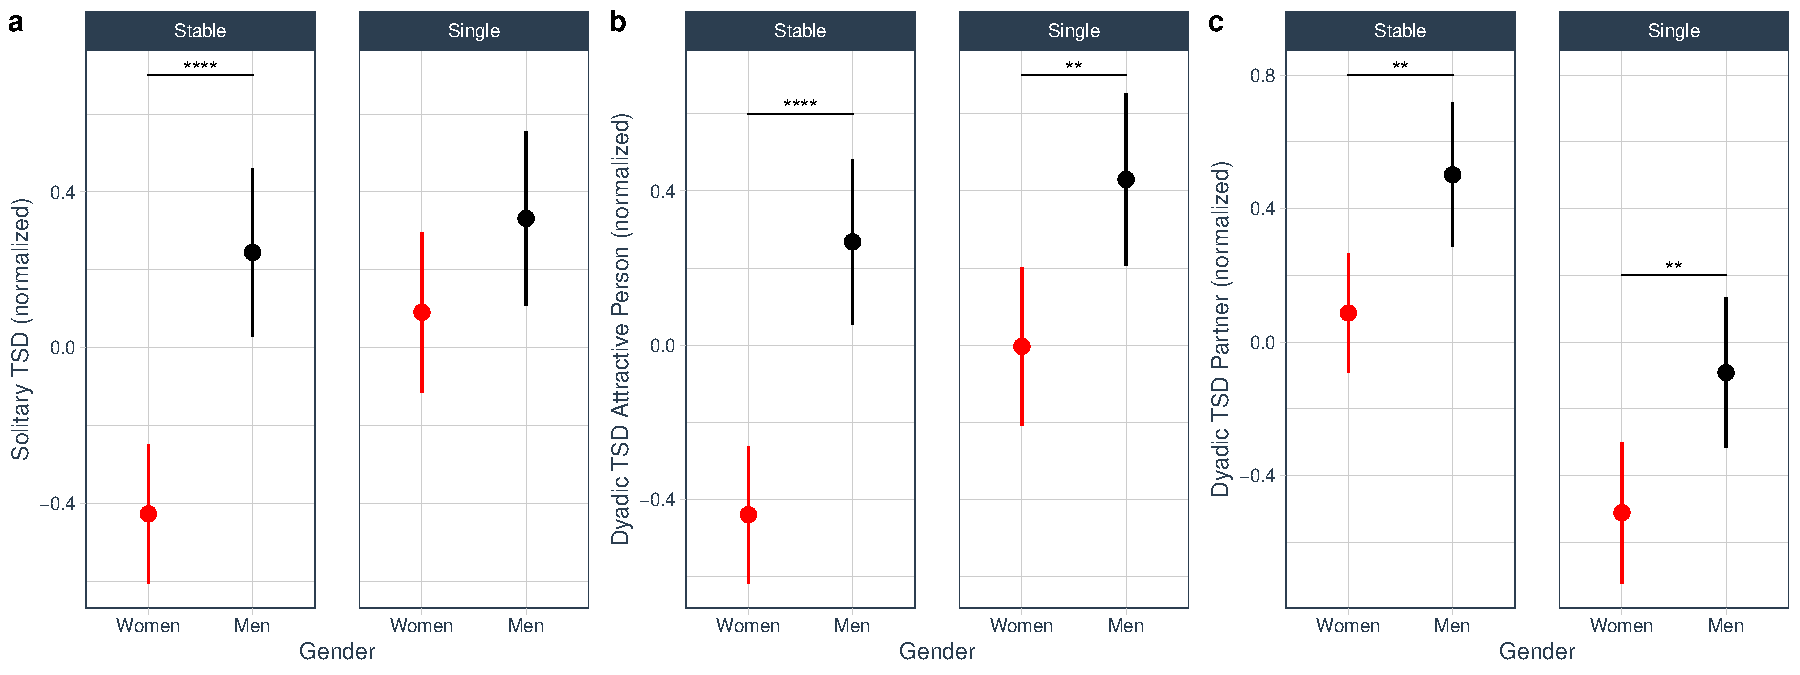
\includegraphics{Sexual_Desire_Arousal_anonymous_files/figure-latex/fig-m1-fin-1.pdf}
\caption{\label{fig:fig-m1-fin}Effects of gender and relationship type on dimensions of Trait Sexual Desire (TSD). All dimensions of TSD were transformed using ordered quantile normalization \autocite{petersonOrderedQuantileNormalization2020a}. \textbf{(a)} Solitary TSD; \textbf{(b)} Dyadic TSD Attractive Person; \textbf{(c)} Dyadic TSD Partner. Dots and bars represent estimated marginal means and 95\% CI. In all cases, significant effects are represented with lines and stars: *\emph{p} \textless{} 0.05, **\emph{p} \textless{} 0.01, ***\emph{p} \textless{} 0.001, ****\emph{p} \textless{} 0.0001.}
\end{figure}

\subsection{Table \ref{tab:tab-m2-fin}. Hypothesis 2}\label{table-reftabtab-m2-fin.-hypothesis-2}

ANOVA-type table for the interaction between \texttt{Relationship\ type}, and \texttt{Gender} for the three final models for hypothesis 2.

\begin{Shaded}
\begin{Highlighting}[]
\CommentTok{\# Generate an ANOVA{-}type table summarizing the effects of relationship type and gender}
\CommentTok{\# on the three final models for Hypothesis 2 (Solitary TSD, Dyadic TSD Attractive Person,}
\CommentTok{\# Dyadic TSD Partner)}
\FunctionTok{bind\_rows}\NormalTok{(}
  \CommentTok{\# ANOVA results for Solitary TSD}
  \FunctionTok{bind\_cols}\NormalTok{(}
    \FunctionTok{anova}\NormalTok{(m2a\_lmer), }\CommentTok{\# Perform ANOVA on the LMM for Solitary TSD}
    \FunctionTok{epsilon\_squared}\NormalTok{(m2a\_lmer) }\CommentTok{\# Compute partial epsilon squared effect sizes}
\NormalTok{  ) }\SpecialCharTok{|\textgreater{}}
    \FunctionTok{mutate}\NormalTok{(}\AttributeTok{DenDF =} \FunctionTok{round}\NormalTok{(DenDF, }\DecValTok{2}\NormalTok{)) }\SpecialCharTok{|\textgreater{}} \CommentTok{\# Round denominator degrees of freedom}
    \FunctionTok{unite}\NormalTok{(}\AttributeTok{col =} \StringTok{"df"}\NormalTok{, NumDF}\SpecialCharTok{:}\NormalTok{DenDF, }\AttributeTok{sep =} \StringTok{", "}\NormalTok{) }\SpecialCharTok{|\textgreater{}} \CommentTok{\# Combine NumDF and DenDF into "df" column}
    \FunctionTok{rownames\_to\_column}\NormalTok{(}\AttributeTok{var =} \StringTok{"Effect"}\NormalTok{) }\SpecialCharTok{|\textgreater{}} \CommentTok{\# Convert row names to a column}
    \FunctionTok{rename}\NormalTok{(}\StringTok{"F"} \OtherTok{=} \StringTok{"F value"}\NormalTok{, }\StringTok{"p"} \OtherTok{=} \StringTok{"Pr(\textgreater{}F)"}\NormalTok{) }\SpecialCharTok{|\textgreater{}} \CommentTok{\# Rename columns for clarity}
    \FunctionTok{select}\NormalTok{(Effect, df, F, p, Epsilon2\_partial) }\SpecialCharTok{|\textgreater{}} \CommentTok{\# Select relevant columns}
    \FunctionTok{mutate}\NormalTok{(}\AttributeTok{p =} \FunctionTok{pval.lev}\NormalTok{(p), }\AttributeTok{Epsilon2\_partial =} \FunctionTok{pe2.lev}\NormalTok{(Epsilon2\_partial)), }\CommentTok{\# Format p{-}values}
  \CommentTok{\# ANOVA results for Dyadic TSD Attractive Person}
  \FunctionTok{bind\_cols}\NormalTok{(}
    \FunctionTok{anova}\NormalTok{(m2b\_lmer),}
    \FunctionTok{epsilon\_squared}\NormalTok{(m2b\_lmer)}
\NormalTok{  ) }\SpecialCharTok{|\textgreater{}}
    \FunctionTok{mutate}\NormalTok{(}\AttributeTok{DenDF =} \FunctionTok{round}\NormalTok{(DenDF, }\DecValTok{2}\NormalTok{)) }\SpecialCharTok{|\textgreater{}}
    \FunctionTok{unite}\NormalTok{(}\AttributeTok{col =} \StringTok{"df"}\NormalTok{, NumDF}\SpecialCharTok{:}\NormalTok{DenDF, }\AttributeTok{sep =} \StringTok{", "}\NormalTok{) }\SpecialCharTok{|\textgreater{}}
    \FunctionTok{rownames\_to\_column}\NormalTok{(}\AttributeTok{var =} \StringTok{"Effect"}\NormalTok{) }\SpecialCharTok{|\textgreater{}}
    \FunctionTok{rename}\NormalTok{(}\StringTok{"F"} \OtherTok{=} \StringTok{"F value"}\NormalTok{, }\StringTok{"p"} \OtherTok{=} \StringTok{"Pr(\textgreater{}F)"}\NormalTok{) }\SpecialCharTok{|\textgreater{}}
    \FunctionTok{select}\NormalTok{(Effect, df, F, p, Epsilon2\_partial) }\SpecialCharTok{|\textgreater{}}
    \FunctionTok{mutate}\NormalTok{(}\AttributeTok{p =} \FunctionTok{pval.lev}\NormalTok{(p), }\AttributeTok{Epsilon2\_partial =} \FunctionTok{pe2.lev}\NormalTok{(Epsilon2\_partial)),}
  \CommentTok{\# ANOVA results for Dyadic TSD Partner}
  \FunctionTok{bind\_cols}\NormalTok{(}
    \FunctionTok{anova}\NormalTok{(m2c\_lmer),}
    \FunctionTok{epsilon\_squared}\NormalTok{(m2c\_lmer)}
\NormalTok{  ) }\SpecialCharTok{|\textgreater{}}
    \FunctionTok{mutate}\NormalTok{(}\AttributeTok{DenDF =} \FunctionTok{round}\NormalTok{(DenDF, }\DecValTok{2}\NormalTok{)) }\SpecialCharTok{|\textgreater{}}
    \FunctionTok{unite}\NormalTok{(}\AttributeTok{col =} \StringTok{"df"}\NormalTok{, NumDF}\SpecialCharTok{:}\NormalTok{DenDF, }\AttributeTok{sep =} \StringTok{", "}\NormalTok{) }\SpecialCharTok{|\textgreater{}}
    \FunctionTok{rownames\_to\_column}\NormalTok{(}\AttributeTok{var =} \StringTok{"Effect"}\NormalTok{) }\SpecialCharTok{|\textgreater{}}
    \FunctionTok{rename}\NormalTok{(}\StringTok{"F"} \OtherTok{=} \StringTok{"F value"}\NormalTok{, }\StringTok{"p"} \OtherTok{=} \StringTok{"Pr(\textgreater{}F)"}\NormalTok{) }\SpecialCharTok{|\textgreater{}}
    \FunctionTok{select}\NormalTok{(Effect, df, F, p, Epsilon2\_partial) }\SpecialCharTok{|\textgreater{}}
    \FunctionTok{mutate}\NormalTok{(}\AttributeTok{p =} \FunctionTok{pval.lev}\NormalTok{(p), }\AttributeTok{Epsilon2\_partial =} \FunctionTok{pe2.lev}\NormalTok{(Epsilon2\_partial))}
\NormalTok{) }\SpecialCharTok{|\textgreater{}}
  \CommentTok{\# Format effect names for readability}
  \FunctionTok{mutate}\NormalTok{(}\AttributeTok{Effect =} \FunctionTok{str\_replace\_all}\NormalTok{(Effect, }\StringTok{"}\SpecialCharTok{\textbackslash{}\textbackslash{}}\StringTok{."}\NormalTok{, }\StringTok{" "}\NormalTok{)) }\SpecialCharTok{|\textgreater{}}
  \FunctionTok{mutate}\NormalTok{(}\AttributeTok{Effect =} \FunctionTok{str\_replace\_all}\NormalTok{(Effect, }\StringTok{":"}\NormalTok{, }\StringTok{" × "}\NormalTok{)) }\SpecialCharTok{|\textgreater{}}
  \CommentTok{\# Generate a formatted table using \textasciigrave{}kable\textasciigrave{}}
  \FunctionTok{kable}\NormalTok{(}
    \AttributeTok{digits =} \DecValTok{2}\NormalTok{, }\CommentTok{\# Round values to 2 decimal places}
    \AttributeTok{booktabs =} \ConstantTok{TRUE}\NormalTok{, }\CommentTok{\# Use LaTeX booktabs for better formatting}
    \AttributeTok{align =} \FunctionTok{c}\NormalTok{(}\StringTok{"l"}\NormalTok{, }\FunctionTok{rep}\NormalTok{(}\StringTok{"c"}\NormalTok{, }\DecValTok{4}\NormalTok{)), }\CommentTok{\# Align columns}
    \AttributeTok{linesep =} \StringTok{""}\NormalTok{, }\CommentTok{\# No extra lines}
    \AttributeTok{caption =} \StringTok{"Effects of TSD dimensions on SSA Across Gender and Stimuli Sex"}\NormalTok{,}
    \AttributeTok{col.names =} \FunctionTok{c}\NormalTok{(}\StringTok{"Effect"}\NormalTok{, }\StringTok{"$df$"}\NormalTok{, }\StringTok{"$F$"}\NormalTok{, }\StringTok{"$p$"}\NormalTok{, }\StringTok{"$}\SpecialCharTok{\textbackslash{}\textbackslash{}}\StringTok{epsilon\^{}2\_p$"}\NormalTok{), }\CommentTok{\# Column headers}
    \AttributeTok{escape =} \ConstantTok{FALSE} \CommentTok{\# Allow LaTeX formatting}
\NormalTok{  ) }\SpecialCharTok{|\textgreater{}}
  \FunctionTok{kable\_styling}\NormalTok{(}\AttributeTok{latex\_options =} \FunctionTok{c}\NormalTok{(}\StringTok{"HOLD\_position"}\NormalTok{, }\StringTok{"scale\_down"}\NormalTok{)) }\SpecialCharTok{|\textgreater{}} \CommentTok{\# LaTeX table styling}
  \CommentTok{\# Group the table into three sections}
  \FunctionTok{pack\_rows}\NormalTok{(}\StringTok{"Solitary TSD"}\NormalTok{, }\DecValTok{1}\NormalTok{, }\DecValTok{7}\NormalTok{, }
            \AttributeTok{bold =} \ConstantTok{FALSE}\NormalTok{, }\AttributeTok{background =} \StringTok{"lightgray"}\NormalTok{) }\SpecialCharTok{|\textgreater{}}
  \FunctionTok{pack\_rows}\NormalTok{(}\StringTok{"Dyadic TSD Attractive Person"}\NormalTok{, }\DecValTok{8}\NormalTok{, }\DecValTok{14}\NormalTok{, }
            \AttributeTok{bold =} \ConstantTok{FALSE}\NormalTok{, }\AttributeTok{background =} \StringTok{"lightgray"}\NormalTok{) }\SpecialCharTok{|\textgreater{}}
  \FunctionTok{pack\_rows}\NormalTok{(}\StringTok{"Dyadic TSD Partner"}\NormalTok{, }\DecValTok{15}\NormalTok{, }\DecValTok{21}\NormalTok{, }
            \AttributeTok{bold =} \ConstantTok{FALSE}\NormalTok{, }\AttributeTok{background =} \StringTok{"lightgray"}\NormalTok{) }\SpecialCharTok{|\textgreater{}}
  \CommentTok{\# Add footnotes with additional details}
  \FunctionTok{footnote}\NormalTok{(}
    \AttributeTok{general =} \FunctionTok{paste0}\NormalTok{(}
      \StringTok{"Results are type III ANOVA. Solitary TSD: "}\NormalTok{,}
      \StringTok{"$R\^{}2\_\{conditional\}$ = "}\NormalTok{, }\FunctionTok{round}\NormalTok{(}\FunctionTok{r2\_nakagawa}\NormalTok{(m2a\_lmer)}\SpecialCharTok{$}\NormalTok{R2\_conditional, }\DecValTok{3}\NormalTok{),}
      \StringTok{", $R\^{}2\_\{marginal\}$ = "}\NormalTok{, }\FunctionTok{round}\NormalTok{(}\FunctionTok{r2\_nakagawa}\NormalTok{(m2a\_lmer)}\SpecialCharTok{$}\NormalTok{R2\_marginal, }\DecValTok{3}\NormalTok{),}
      \StringTok{"; Dyadic TSD Attractive Person: "}\NormalTok{,}
      \StringTok{"$R\^{}2\_\{conditional\}$ = "}\NormalTok{, }\FunctionTok{round}\NormalTok{(}\FunctionTok{r2\_nakagawa}\NormalTok{(m2b\_lmer)}\SpecialCharTok{$}\NormalTok{R2\_conditional, }\DecValTok{3}\NormalTok{),}
      \StringTok{", $R\^{}2\_\{marginal\}$ = "}\NormalTok{, }\FunctionTok{round}\NormalTok{(}\FunctionTok{r2\_nakagawa}\NormalTok{(m2b\_lmer)}\SpecialCharTok{$}\NormalTok{R2\_marginal, }\DecValTok{3}\NormalTok{),}
      \StringTok{"; Dyadic TSD Partner: "}\NormalTok{,}
      \StringTok{"$R\^{}2\_\{conditional\}$ = "}\NormalTok{, }\FunctionTok{round}\NormalTok{(}\FunctionTok{r2\_nakagawa}\NormalTok{(m2c\_lmer)}\SpecialCharTok{$}\NormalTok{R2\_conditional, }\DecValTok{3}\NormalTok{),}
      \StringTok{", $R\^{}2\_\{marginal\}$ = "}\NormalTok{, }\FunctionTok{round}\NormalTok{(}\FunctionTok{r2\_nakagawa}\NormalTok{(m2c\_lmer)}\SpecialCharTok{$}\NormalTok{R2\_marginal, }\DecValTok{3}\NormalTok{),}
      \StringTok{". Gender = participant gender (women, men); Stimuli sex = sex of stimuli (male, female).}
\StringTok{      Partial epsilon squared ($}\SpecialCharTok{\textbackslash{}\textbackslash{}\textbackslash{}\textbackslash{}}\StringTok{epsilon\^{}2\_p$) is used as an effect size, as it provides}
\StringTok{      a less biased estimate than $}\SpecialCharTok{\textbackslash{}\textbackslash{}\textbackslash{}\textbackslash{}}\StringTok{eta\^{}2$ (see }\SpecialCharTok{\textbackslash{}\textbackslash{}\textbackslash{}\textbackslash{}}\StringTok{cite\{albersWhenPowerAnalyses2018\}).}
\StringTok{      Significant effects are in bold."}
\NormalTok{    ),}
    \AttributeTok{escape =} \ConstantTok{FALSE}\NormalTok{, }\CommentTok{\# Allow LaTeX formatting}
    \AttributeTok{threeparttable =} \ConstantTok{TRUE}\NormalTok{,}
    \AttributeTok{footnote\_as\_chunk =} \ConstantTok{TRUE}
\NormalTok{  )}
\end{Highlighting}
\end{Shaded}

\begin{table}[H]
\centering
\caption{\label{tab:tab-m2-fin}Effects of TSD dimensions on SSA Across Gender and Stimuli Sex}
\centering
\resizebox{\ifdim\width>\linewidth\linewidth\else\width\fi}{!}{
\begin{threeparttable}
\begin{tabular}[t]{lcccc}
\toprule
Effect & $df$ & $F$ & $p$ & $\epsilon^2_p$\\
\midrule
\addlinespace[0.3em]
\multicolumn{5}{l}{\cellcolor{lightgray}{Solitary TSD}}\\
\hspace{1em}Solitary TSD & 1, 319 & 17.46 & \textbf{< 0.0001} & 0.0489\\
\hspace{1em}Gender & 1, 319 & 8.84 & \textbf{0.0032} & 0.0239\\
\hspace{1em}Stimuli sex & 1, 369.21 & 24.71 & \textbf{< 0.0001} & 0.06\\
\hspace{1em}Solitary TSD × Gender & 1, 319 & 0.85 & 0.36 & < 0.0001\\
\hspace{1em}Solitary TSD × Stimuli sex & 1, 319 & 0.02 & 0.88 & < 0.0001\\
\hspace{1em}Gender × Stimuli sex & 1, 319 & 74.79 & \textbf{< 0.0001} & 0.19\\
\hspace{1em}Solitary TSD × Gender × Stimuli sex & 1, 319 & 1.78 & 0.18 & 0.0024\\
\addlinespace[0.3em]
\multicolumn{5}{l}{\cellcolor{lightgray}{Dyadic TSD Attractive Person}}\\
\hspace{1em}Dyadic TSD Attractive Person & 1, 319 & 48.49 & \textbf{< 0.0001} & 0.13\\
\hspace{1em}Gender & 1, 319 & 1.45 & 0.23 & 0.0014\\
\hspace{1em}Stimuli sex & 1, 373.93 & 2.69 & 0.1 & 0.0045\\
\hspace{1em}Dyadic TSD Attractive Person × Gender & 1, 319 & 0.53 & 0.47 & < 0.0001\\
\hspace{1em}Dyadic TSD Attractive Person × Stimuli sex & 1, 319 & 15.43 & \textbf{< 0.001} & 0.0431\\
\hspace{1em}Gender × Stimuli sex & 1, 319 & 27.44 & \textbf{< 0.0001} & 0.08\\
\hspace{1em}Dyadic TSD Attractive Person × Gender × Stimuli sex & 1, 319 & 29.69 & \textbf{< 0.0001} & 0.08\\
\addlinespace[0.3em]
\multicolumn{5}{l}{\cellcolor{lightgray}{Dyadic TSD Partner}}\\
\hspace{1em}Dyadic TSD Partner & 1, 316 & 6.59 & \textbf{0.0107} & 0.0173\\
\hspace{1em}Gender & 1, 316 & 0.03 & 0.85 & < 0.0001\\
\hspace{1em}Stimuli sex & 1, 344.42 & 0.99 & 0.32 & < 0.0001\\
\hspace{1em}Dyadic TSD Partner × Gender & 1, 316 & 3.97 & \textbf{0.0472} & 0.0093\\
\hspace{1em}Dyadic TSD Partner × Stimuli sex & 1, 316 & 8.46 & \textbf{0.0039} & 0.023\\
\hspace{1em}Gender × Stimuli sex & 1, 316 & 20.55 & \textbf{< 0.0001} & 0.06\\
\hspace{1em}Dyadic TSD Partner × Gender × Stimuli sex & 1, 316 & 5.70 & \textbf{0.0176} & 0.0146\\
\bottomrule
\end{tabular}
\begin{tablenotes}[para]
\item \textit{Note: } 
\item Results are type III ANOVA. Solitary TSD: $R^2_{conditional}$ = 0.745, $R^2_{marginal}$ = 0.335; Dyadic TSD Attractive Person: $R^2_{conditional}$ = 0.745, $R^2_{marginal}$ = 0.367; Dyadic TSD Partner: $R^2_{conditional}$ = 0.745, $R^2_{marginal}$ = 0.329. Gender = participant gender (women, men); Stimuli sex = sex of stimuli (male, female).
      Partial epsilon squared ($\epsilon^2_p$) is used as an effect size, as it provides
      a less biased estimate than $\eta^2$ (see \cite{albersWhenPowerAnalyses2018}).
      Significant effects are in bold.
\end{tablenotes}
\end{threeparttable}}
\end{table}

\subsection{Figure \ref{fig:fig-m2-fin}. Hypothesis 2}\label{figure-reffigfig-m2-fin.-hypothesis-2}

Simple slopes for the interaction between dimensions of sexual desire and \texttt{Stimuli\ Sex}, by gender, for the three final models for hypothesis 2.

\begin{Shaded}
\begin{Highlighting}[]
\CommentTok{\# Generate a combined figure showing the interaction between sexual desire dimensions}
\CommentTok{\# and stimuli sex, grouped by gender, for the final models in Hypothesis 2}
\FunctionTok{ggarrange}\NormalTok{(}
\NormalTok{  p\_m2a.fin, }\CommentTok{\# Solitary TSD simple slopes plot}
\NormalTok{  p\_m2b.fin, }\CommentTok{\# Dyadic TSD Attractive Person simple slopes plot}
\NormalTok{  p\_m2c.fin, }\CommentTok{\# Dyadic TSD Partner simple slopes plot}
  \AttributeTok{common.legend =} \ConstantTok{TRUE}\NormalTok{, }\CommentTok{\# Use a shared legend across all plots}
  \AttributeTok{legend =} \StringTok{"bottom"}\NormalTok{, }\CommentTok{\# Position the legend at the bottom}
  \AttributeTok{labels =} \StringTok{"auto"}\NormalTok{, }\CommentTok{\# Automatically label subfigures (a, b, c)}
  \AttributeTok{nrow =} \DecValTok{3}\NormalTok{, }\CommentTok{\# Arrange plots in three rows}
  \AttributeTok{ncol =} \DecValTok{1} \CommentTok{\# Use a single column layout}
\NormalTok{)}
\end{Highlighting}
\end{Shaded}

\begin{figure}
\centering
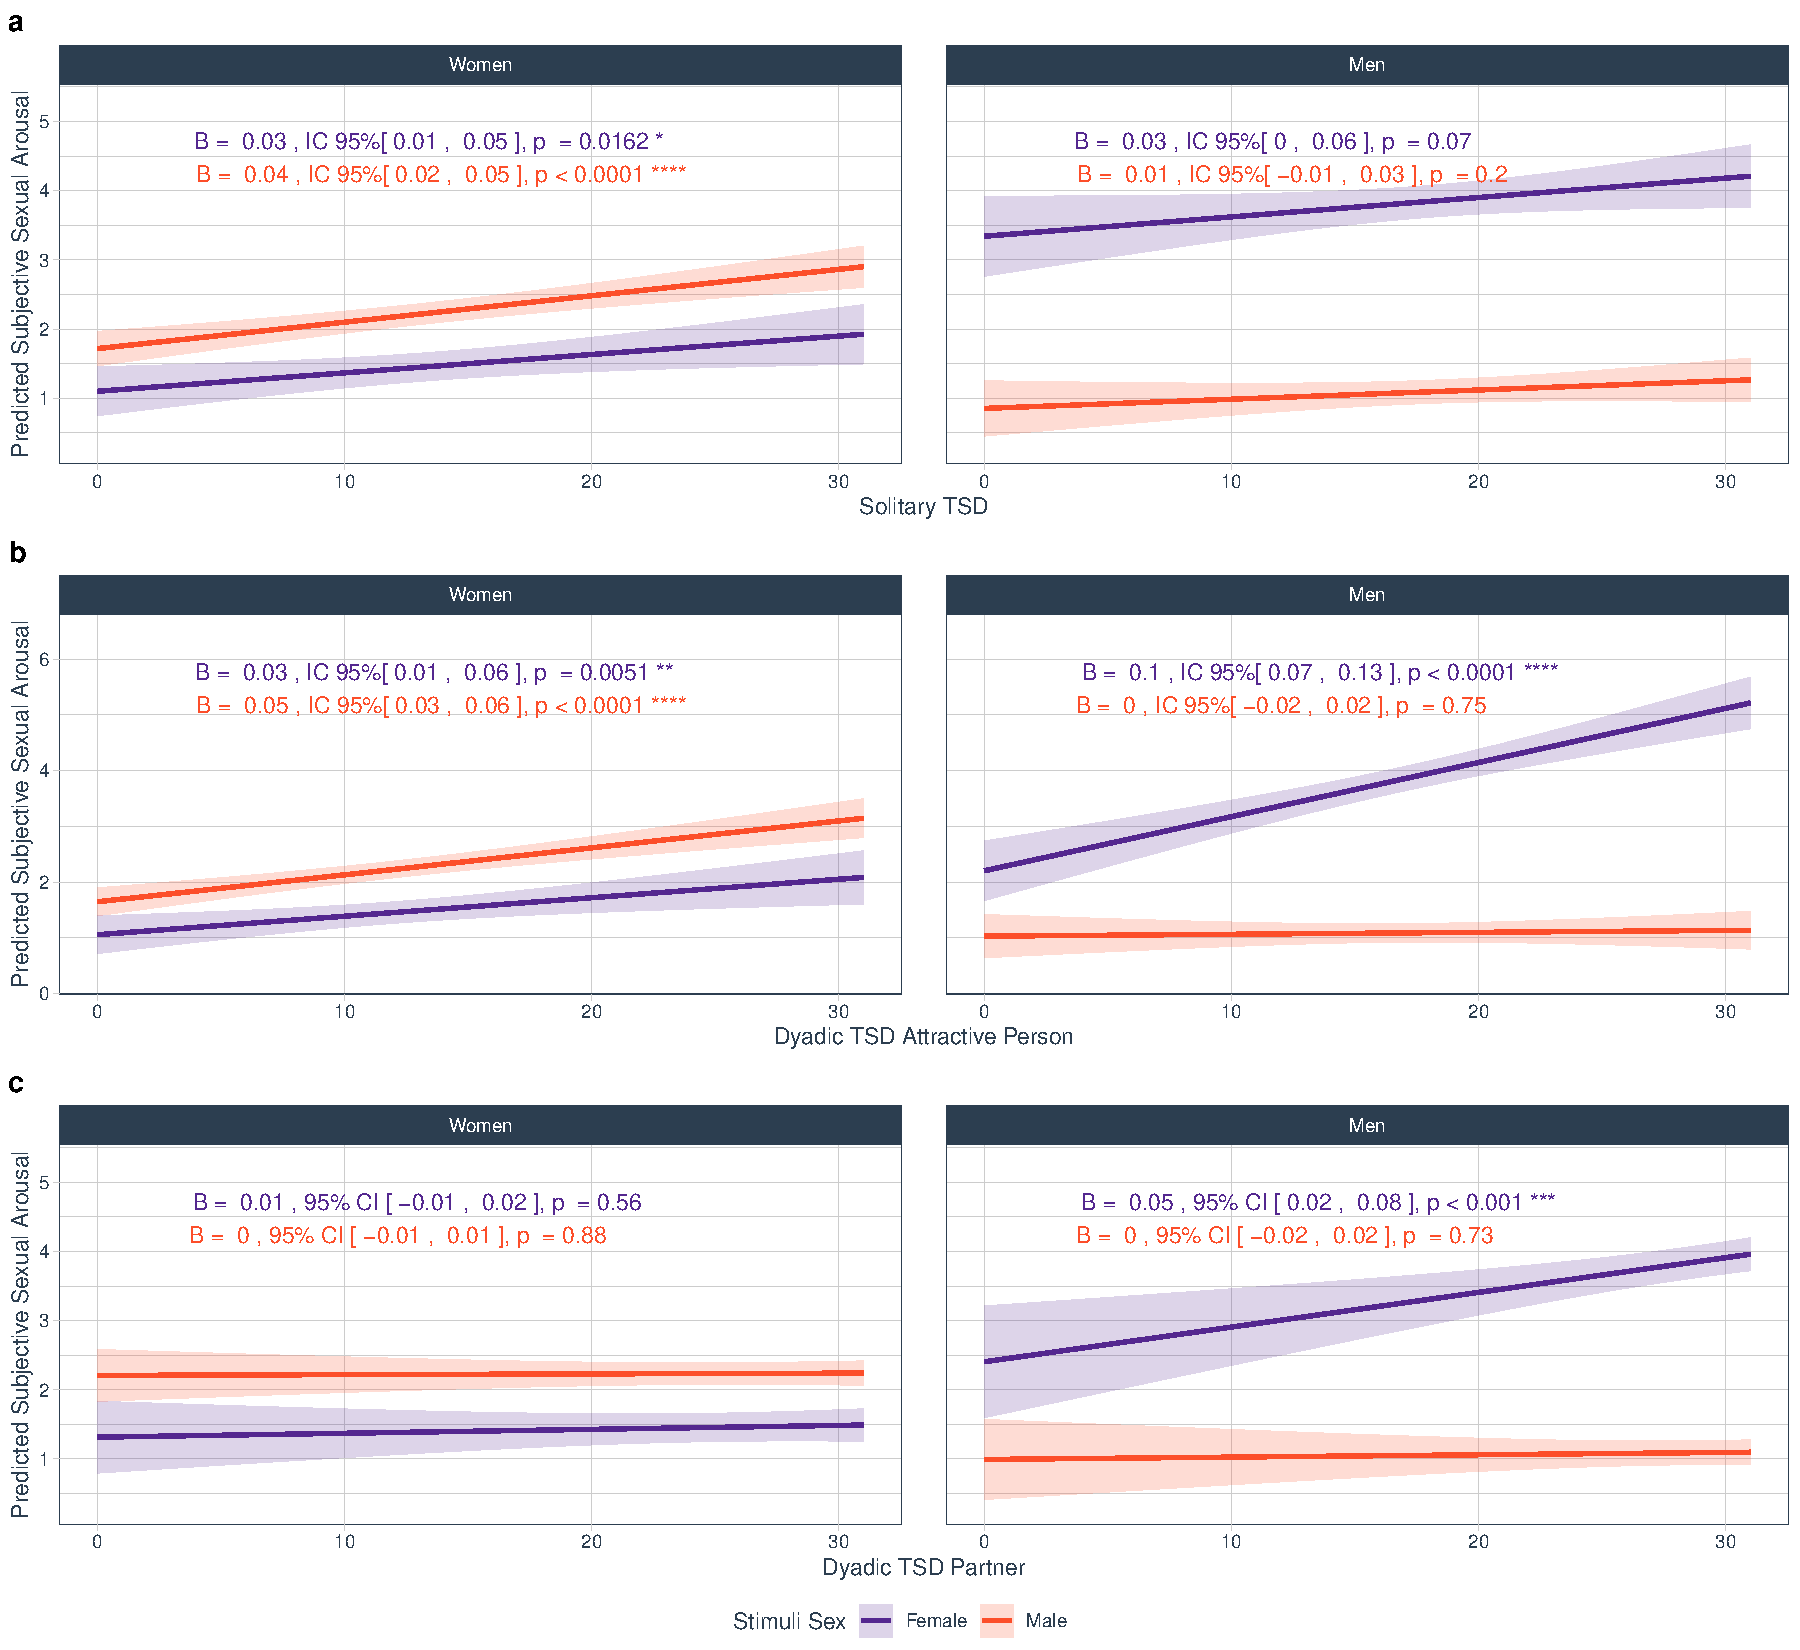
\includegraphics{Sexual_Desire_Arousal_anonymous_files/figure-latex/fig-m2-fin-1.pdf}
\caption{\label{fig:fig-m2-fin}Slopes of Trait Sexual Desire (TSD) dimensions on sexual arousal, by gender and stimuli sex. \textbf{(a)} Solitary TSD; \textbf{(b)} Dyadic TSD Attractive Person; \textbf{(c)} Dyadic TSD Partner. Lines represent simple slopes and 95\% CI. Significant effects are represented with stars alongside slope details: *\emph{p} \textless{} 0.05, **\emph{p} \textless{} 0.01, ***\emph{p} \textless{} 0.001, ****\emph{p} \textless{} 0.0001.}
\end{figure}

\subsection{Table \ref{tab:tab-m3-fin}. Hypothesis 3}\label{table-reftabtab-m3-fin.-hypothesis-3}

ANOVA-type table for the interaction between \texttt{Relationship\ type}, and \texttt{Gender} for the three final models for hypothesis 3.

\begin{Shaded}
\begin{Highlighting}[]
\CommentTok{\# Generate an ANOVA{-}type table summarizing the interaction between}
\CommentTok{\# Relationship Type and Gender for Hypothesis 3 models}
\FunctionTok{bind\_rows}\NormalTok{(}
  \CommentTok{\# Model 3a: Solitary TSD}
  \FunctionTok{bind\_cols}\NormalTok{(}\FunctionTok{anova}\NormalTok{(m3a\_lmer), }\FunctionTok{epsilon\_squared}\NormalTok{(m3a\_lmer)) }\SpecialCharTok{|\textgreater{}}
    \FunctionTok{mutate}\NormalTok{(}\AttributeTok{DenDF =} \FunctionTok{round}\NormalTok{(DenDF, }\DecValTok{2}\NormalTok{)) }\SpecialCharTok{|\textgreater{}} \CommentTok{\# Round denominator degrees of freedom}
    \FunctionTok{unite}\NormalTok{(}\AttributeTok{col =} \StringTok{"df"}\NormalTok{, NumDF}\SpecialCharTok{:}\NormalTok{DenDF, }\AttributeTok{sep =} \StringTok{", "}\NormalTok{) }\SpecialCharTok{|\textgreater{}} \CommentTok{\# Combine NumDF and DenDF into one column}
    \FunctionTok{rownames\_to\_column}\NormalTok{(}\AttributeTok{var =} \StringTok{"Effect"}\NormalTok{) }\SpecialCharTok{|\textgreater{}} \CommentTok{\# Convert row names to a column}
    \FunctionTok{rename}\NormalTok{(}\StringTok{"F"} \OtherTok{=} \StringTok{"F value"}\NormalTok{, }\StringTok{"p"} \OtherTok{=} \StringTok{"Pr(\textgreater{}F)"}\NormalTok{) }\SpecialCharTok{|\textgreater{}} \CommentTok{\# Rename columns for clarity}
    \FunctionTok{select}\NormalTok{(Effect, df, F, p, Epsilon2\_partial) }\SpecialCharTok{|\textgreater{}} \CommentTok{\# Keep relevant columns}
    \FunctionTok{mutate}\NormalTok{(}\AttributeTok{p =} \FunctionTok{pval.lev}\NormalTok{(p), }\AttributeTok{Epsilon2\_partial =} \FunctionTok{pe2.lev}\NormalTok{(Epsilon2\_partial)),}
  \CommentTok{\# Model 3b: Dyadic TSD Attractive Person}
  \FunctionTok{bind\_cols}\NormalTok{(}\FunctionTok{anova}\NormalTok{(m3b\_lmer), }\FunctionTok{epsilon\_squared}\NormalTok{(m3b\_lmer)) }\SpecialCharTok{|\textgreater{}}
    \FunctionTok{mutate}\NormalTok{(}\AttributeTok{DenDF =} \FunctionTok{round}\NormalTok{(DenDF, }\DecValTok{2}\NormalTok{)) }\SpecialCharTok{|\textgreater{}}
    \FunctionTok{unite}\NormalTok{(}\AttributeTok{col =} \StringTok{"df"}\NormalTok{, NumDF}\SpecialCharTok{:}\NormalTok{DenDF, }\AttributeTok{sep =} \StringTok{", "}\NormalTok{) }\SpecialCharTok{|\textgreater{}}
    \FunctionTok{rownames\_to\_column}\NormalTok{(}\AttributeTok{var =} \StringTok{"Effect"}\NormalTok{) }\SpecialCharTok{|\textgreater{}}
    \FunctionTok{rename}\NormalTok{(}\StringTok{"F"} \OtherTok{=} \StringTok{"F value"}\NormalTok{, }\StringTok{"p"} \OtherTok{=} \StringTok{"Pr(\textgreater{}F)"}\NormalTok{) }\SpecialCharTok{|\textgreater{}}
    \FunctionTok{select}\NormalTok{(Effect, df, F, p, Epsilon2\_partial) }\SpecialCharTok{|\textgreater{}}
    \FunctionTok{mutate}\NormalTok{(}\AttributeTok{p =} \FunctionTok{pval.lev}\NormalTok{(p), }\AttributeTok{Epsilon2\_partial =} \FunctionTok{pe2.lev}\NormalTok{(Epsilon2\_partial)),}
  \CommentTok{\# Model 3c: Dyadic TSD Partner}
  \FunctionTok{bind\_cols}\NormalTok{(}\FunctionTok{anova}\NormalTok{(m3c\_lmer), }\FunctionTok{epsilon\_squared}\NormalTok{(m3c\_lmer)) }\SpecialCharTok{|\textgreater{}}
    \FunctionTok{mutate}\NormalTok{(}\AttributeTok{DenDF =} \FunctionTok{round}\NormalTok{(DenDF, }\DecValTok{2}\NormalTok{)) }\SpecialCharTok{|\textgreater{}}
    \FunctionTok{unite}\NormalTok{(}\AttributeTok{col =} \StringTok{"df"}\NormalTok{, NumDF}\SpecialCharTok{:}\NormalTok{DenDF, }\AttributeTok{sep =} \StringTok{", "}\NormalTok{) }\SpecialCharTok{|\textgreater{}}
    \FunctionTok{rownames\_to\_column}\NormalTok{(}\AttributeTok{var =} \StringTok{"Effect"}\NormalTok{) }\SpecialCharTok{|\textgreater{}}
    \FunctionTok{rename}\NormalTok{(}\StringTok{"F"} \OtherTok{=} \StringTok{"F value"}\NormalTok{, }\StringTok{"p"} \OtherTok{=} \StringTok{"Pr(\textgreater{}F)"}\NormalTok{) }\SpecialCharTok{|\textgreater{}}
    \FunctionTok{select}\NormalTok{(Effect, df, F, p, Epsilon2\_partial) }\SpecialCharTok{|\textgreater{}}
    \FunctionTok{mutate}\NormalTok{(}\AttributeTok{p =} \FunctionTok{pval.lev}\NormalTok{(p), }\AttributeTok{Epsilon2\_partial =} \FunctionTok{pe2.lev}\NormalTok{(Epsilon2\_partial))}
\NormalTok{) }\SpecialCharTok{|\textgreater{}}
  \FunctionTok{mutate}\NormalTok{(}\AttributeTok{Effect =} \FunctionTok{str\_replace\_all}\NormalTok{(Effect, }\StringTok{"}\SpecialCharTok{\textbackslash{}\textbackslash{}}\StringTok{."}\NormalTok{, }\StringTok{" "}\NormalTok{)) }\SpecialCharTok{|\textgreater{}} \CommentTok{\# Replace dots with spaces}
  \FunctionTok{mutate}\NormalTok{(}\AttributeTok{Effect =} \FunctionTok{str\_replace\_all}\NormalTok{(Effect, }\StringTok{":"}\NormalTok{, }\StringTok{" × "}\NormalTok{)) }\SpecialCharTok{|\textgreater{}} \CommentTok{\# Replace colons with ×}
  \CommentTok{\# Format table output}
  \FunctionTok{kable}\NormalTok{(}
    \AttributeTok{digits =} \DecValTok{2}\NormalTok{, }\AttributeTok{booktabs =} \ConstantTok{TRUE}\NormalTok{, }\AttributeTok{align =} \FunctionTok{c}\NormalTok{(}\StringTok{"l"}\NormalTok{, }\FunctionTok{rep}\NormalTok{(}\StringTok{"c"}\NormalTok{, }\DecValTok{4}\NormalTok{)),}
    \AttributeTok{linesep =} \StringTok{""}\NormalTok{, }\AttributeTok{caption =} \StringTok{"Effects of TSD dimensions on SSA across Gender and }
\StringTok{    Relationship Status"}\NormalTok{,}
    \AttributeTok{col.names =} \FunctionTok{c}\NormalTok{(}\StringTok{"Effect"}\NormalTok{, }\StringTok{"$df$"}\NormalTok{, }\StringTok{"$F$"}\NormalTok{, }\StringTok{"$p$"}\NormalTok{, }\StringTok{"$}\SpecialCharTok{\textbackslash{}\textbackslash{}}\StringTok{epsilon\^{}2\_p$"}\NormalTok{), }\AttributeTok{escape =} \ConstantTok{FALSE}
\NormalTok{  ) }\SpecialCharTok{|\textgreater{}}
  \FunctionTok{kable\_styling}\NormalTok{(}\AttributeTok{latex\_options =} \FunctionTok{c}\NormalTok{(}\StringTok{"HOLD\_position"}\NormalTok{, }\StringTok{"scale\_down"}\NormalTok{)) }\SpecialCharTok{|\textgreater{}}
  \CommentTok{\# Add section grouping for each model}
  \FunctionTok{pack\_rows}\NormalTok{(}\StringTok{"Solitary TSD"}\NormalTok{, }\DecValTok{1}\NormalTok{, }\DecValTok{7}\NormalTok{, }
            \AttributeTok{bold =} \ConstantTok{FALSE}\NormalTok{, }\AttributeTok{background =} \StringTok{"lightgray"}\NormalTok{) }\SpecialCharTok{|\textgreater{}}
  \FunctionTok{pack\_rows}\NormalTok{(}\StringTok{"Dyadic TSD Attractive Person"}\NormalTok{, }\DecValTok{8}\NormalTok{, }\DecValTok{14}\NormalTok{, }
            \AttributeTok{bold =} \ConstantTok{FALSE}\NormalTok{, }\AttributeTok{background =} \StringTok{"lightgray"}\NormalTok{) }\SpecialCharTok{|\textgreater{}}
  \FunctionTok{pack\_rows}\NormalTok{(}\StringTok{"Dyadic TSD Partner"}\NormalTok{, }\DecValTok{15}\NormalTok{, }\DecValTok{21}\NormalTok{, }
            \AttributeTok{bold =} \ConstantTok{FALSE}\NormalTok{, }\AttributeTok{background =} \StringTok{"lightgray"}\NormalTok{) }\SpecialCharTok{|\textgreater{}}
  \CommentTok{\# Add footnote with additional model details}
  \FunctionTok{footnote}\NormalTok{(}
    \AttributeTok{general =} \FunctionTok{paste0}\NormalTok{(}
      \StringTok{"Results are type III ANOVA. "}\NormalTok{,}
      \StringTok{"Solitary TSD: $R\^{}2\_\{conditional\}$ = "}\NormalTok{, }\FunctionTok{round}\NormalTok{(}\FunctionTok{r2\_nakagawa}\NormalTok{(m3a\_lmer)}\SpecialCharTok{$}\NormalTok{R2\_conditional, }\DecValTok{3}\NormalTok{),}
      \StringTok{", $R\^{}2\_\{marginal\}$ = "}\NormalTok{, }\FunctionTok{round}\NormalTok{(}\FunctionTok{r2\_nakagawa}\NormalTok{(m3a\_lmer)}\SpecialCharTok{$}\NormalTok{R2\_marginal, }\DecValTok{3}\NormalTok{),}
      \StringTok{"; Dyadic TSD Attractive Person: $R\^{}2\_\{conditional\}$ = "}\NormalTok{,}
      \FunctionTok{round}\NormalTok{(}\FunctionTok{r2\_nakagawa}\NormalTok{(m3b\_lmer)}\SpecialCharTok{$}\NormalTok{R2\_conditional, }\DecValTok{3}\NormalTok{),}
      \StringTok{", $R\^{}2\_\{marginal\}$ = "}\NormalTok{, }\FunctionTok{round}\NormalTok{(}\FunctionTok{r2\_nakagawa}\NormalTok{(m3b\_lmer)}\SpecialCharTok{$}\NormalTok{R2\_marginal, }\DecValTok{3}\NormalTok{),}
      \StringTok{"; Dyadic TSD {-} Partner: $R\^{}2\_\{conditional\}$ = "}\NormalTok{,}
      \FunctionTok{round}\NormalTok{(}\FunctionTok{r2\_nakagawa}\NormalTok{(m3c\_lmer)}\SpecialCharTok{$}\NormalTok{R2\_conditional, }\DecValTok{3}\NormalTok{),}
      \StringTok{", $R\^{}2\_\{marginal\}$ = "}\NormalTok{, }\FunctionTok{round}\NormalTok{(}\FunctionTok{r2\_nakagawa}\NormalTok{(m3c\_lmer)}\SpecialCharTok{$}\NormalTok{R2\_marginal, }\DecValTok{3}\NormalTok{),}
      \StringTok{". Gender = participants\textquotesingle{} gender (women, men); Relationship = relationship type}
\StringTok{      (stable, single). As effect size, we report partial epsilon squared ($}\SpecialCharTok{\textbackslash{}\textbackslash{}\textbackslash{}\textbackslash{}}\StringTok{epsilon\^{}2\_p$),}
\StringTok{      which provides a less biased estimate than $}\SpecialCharTok{\textbackslash{}\textbackslash{}\textbackslash{}\textbackslash{}}\StringTok{eta\^{}2$ }
\StringTok{      (see }\SpecialCharTok{\textbackslash{}\textbackslash{}\textbackslash{}\textbackslash{}}\StringTok{cite\{albersWhenPowerAnalyses2018\}). Significant effects are in bold."}
\NormalTok{    ),}
    \AttributeTok{escape =} \ConstantTok{FALSE}\NormalTok{, }\AttributeTok{threeparttable =} \ConstantTok{TRUE}\NormalTok{, }\AttributeTok{footnote\_as\_chunk =} \ConstantTok{TRUE}
\NormalTok{  )}
\end{Highlighting}
\end{Shaded}

\begin{table}[H]
\centering
\caption{\label{tab:tab-m3-fin}Effects of TSD dimensions on SSA across Gender and 
    Relationship Status}
\centering
\resizebox{\ifdim\width>\linewidth\linewidth\else\width\fi}{!}{
\begin{threeparttable}
\begin{tabular}[t]{lcccc}
\toprule
Effect & $df$ & $F$ & $p$ & $\epsilon^2_p$\\
\midrule
\addlinespace[0.3em]
\multicolumn{5}{l}{\cellcolor{lightgray}{Solitary TSD}}\\
\hspace{1em}Solitary TSD & 1, 315 & 6.88 & \textbf{0.0091} & 0.0183\\
\hspace{1em}Gender & 1, 355.34 & 14.10 & \textbf{< 0.001} & 0.0355\\
\hspace{1em}Relationship & 1, 314.95 & 0.34 & 0.56 & < 0.0001\\
\hspace{1em}Solitary TSD × Gender & 1, 315.23 & 0.07 & 0.79 & < 0.0001\\
\hspace{1em}Solitary TSD × Relationship & 1, 314.95 & 0.53 & 0.47 & < 0.0001\\
\hspace{1em}Gender × Relationship & 1, 314.95 & 2.95 & 0.09 & 0.0061\\
\hspace{1em}Solitary TSD × Gender × Relationship & 1, 315.08 & 2.02 & 0.16 & 0.0032\\
\addlinespace[0.3em]
\multicolumn{5}{l}{\cellcolor{lightgray}{Dyadic TSD Attractive Person}}\\
\hspace{1em}Dyadic TSD Attractive Person & 1, 315.21 & 46.80 & \textbf{< 0.0001} & 0.13\\
\hspace{1em}Gender & 1, 354.77 & 1.21 & 0.27 & < 0.001\\
\hspace{1em}Relationship & 1, 315.16 & 0.13 & 0.72 & < 0.0001\\
\hspace{1em}Dyadic TSD Attractive Person × Gender & 1, 314.97 & 7.06 & \textbf{0.0083} & 0.0188\\
\hspace{1em}Dyadic TSD Attractive Person × Relationship & 1, 315.21 & 0.08 & 0.77 & < 0.0001\\
\hspace{1em}Gender × Relationship & 1, 315.06 & 0.00 & 0.97 & < 0.0001\\
\hspace{1em}Dyadic TSD Attractive Person × Gender × Relationship & 1, 314.97 & 0.34 & 0.56 & < 0.0001\\
\addlinespace[0.3em]
\multicolumn{5}{l}{\cellcolor{lightgray}{Dyadic TSD Partner}}\\
\hspace{1em}Dyadic TSD Partner & 1, 311.9 & 3.16 & 0.08 & 0.0069\\
\hspace{1em}Gender & 1, 328.45 & 2.50 & 0.11 & 0.0045\\
\hspace{1em}Relationship & 1, 311.9 & 0.67 & 0.41 & < 0.0001\\
\hspace{1em}Dyadic TSD Partner × Gender & 1, 311.98 & 1.15 & 0.28 & < 0.001\\
\hspace{1em}Dyadic TSD Partner × Relationship & 1, 311.9 & 1.37 & 0.24 & 0.0012\\
\hspace{1em}Gender × Relationship & 1, 311.9 & 8.51 & \textbf{0.0038} & 0.0234\\
\hspace{1em}Dyadic TSD Partner × Gender × Relationship & 1, 311.94 & 8.31 & \textbf{0.0042} & 0.0228\\
\bottomrule
\end{tabular}
\begin{tablenotes}[para]
\item \textit{Note: } 
\item Results are type III ANOVA. Solitary TSD: $R^2_{conditional}$ = 0.72, $R^2_{marginal}$ = 0.171; Dyadic TSD Attractive Person: $R^2_{conditional}$ = 0.719, $R^2_{marginal}$ = 0.225; Dyadic TSD - Partner: $R^2_{conditional}$ = 0.719, $R^2_{marginal}$ = 0.182. Gender = participants' gender (women, men); Relationship = relationship type
      (stable, single). As effect size, we report partial epsilon squared ($\epsilon^2_p$),
      which provides a less biased estimate than $\eta^2$ 
      (see \cite{albersWhenPowerAnalyses2018}). Significant effects are in bold.
\end{tablenotes}
\end{threeparttable}}
\end{table}

\subsection{Figure \ref{fig:fig-m3-fin}. Hypothesis 3}\label{figure-reffigfig-m3-fin.-hypothesis-3}

Simple slopes for the interaction between dimensions of sexual desire and \texttt{Stimuli\ Sex}, by gender, for the three final models for hypothesis 3.

\begin{Shaded}
\begin{Highlighting}[]
\CommentTok{\# Generate a combined figure for Hypothesis 3}
\CommentTok{\# This figure shows simple slopes for sexual desire dimensions on sexual arousal}
\FunctionTok{ggarrange}\NormalTok{(}
\NormalTok{  p\_m3a.fin, p\_m3b.fin, p\_m3c.fin, }\CommentTok{\# Arrange the three model plots}
  \AttributeTok{common.legend =} \ConstantTok{TRUE}\NormalTok{, }\CommentTok{\# Use a shared legend for all subplots}
  \AttributeTok{legend =} \StringTok{"bottom"}\NormalTok{, }\CommentTok{\# Position the legend below the plots}
  \AttributeTok{labels =} \StringTok{"auto"}\NormalTok{, }\CommentTok{\# Automatically label subplots as (a), (b), (c)}
  \AttributeTok{nrow =} \DecValTok{3}\NormalTok{, }\CommentTok{\# Arrange in three rows}
  \AttributeTok{ncol =} \DecValTok{1} \CommentTok{\# Single column layout}
\NormalTok{)}
\end{Highlighting}
\end{Shaded}

\begin{figure}
\centering
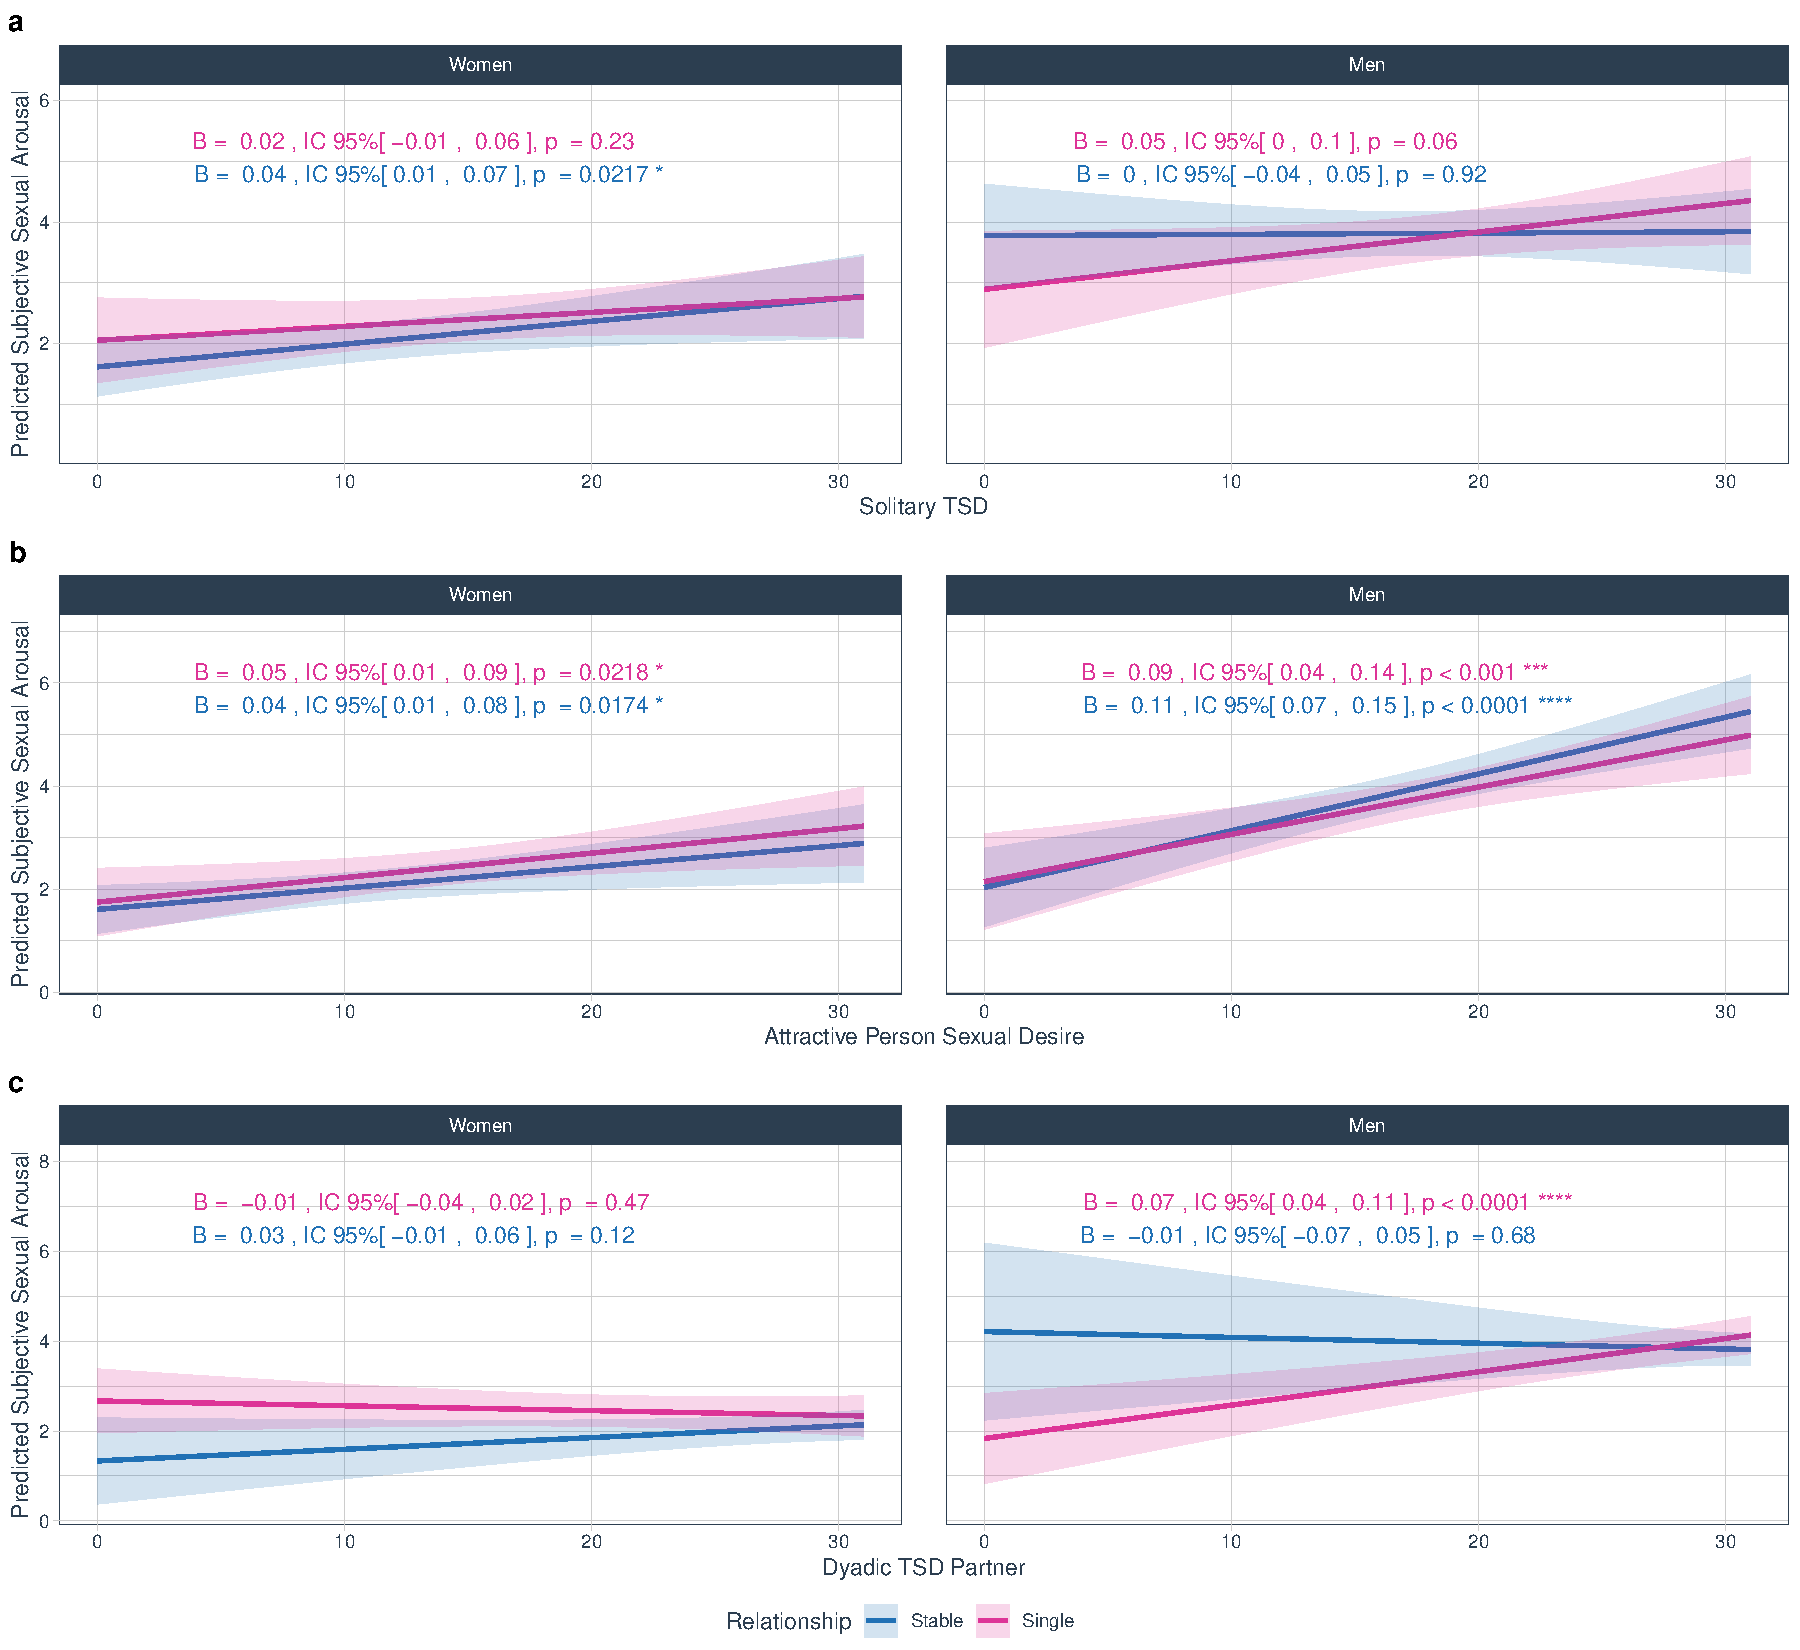
\includegraphics{Sexual_Desire_Arousal_anonymous_files/figure-latex/fig-m3-fin-1.pdf}
\caption{\label{fig:fig-m3-fin}Slopes of Trait Sexual Desire (TSD) dimensions on sexual arousal, by gender and relationship status. \textbf{(a)} Solitary TSD; \textbf{(b)} Dyadic TSD Attractive Person; \textbf{(c)} Dyadic TSD Partner. Lines represent simple slopes and 95\% CI. Significant effects are represented with stars alongside slope details: *\emph{p} \textless{} 0.05, **\emph{p} \textless{} 0.01, ***\emph{p} \textless{} 0.001, ****\emph{p} \textless{} 0.0001.}
\end{figure}

\begin{center}\rule{0.5\linewidth}{0.5pt}\end{center}

\section{Session info (for reproducibility)}\label{session}

\begin{Shaded}
\begin{Highlighting}[]
\CommentTok{\# Display session information for reproducibility}
\CommentTok{\# {-} Uses \textasciigrave{}pander()\textasciigrave{} for better formatting}
\CommentTok{\# {-} \textasciigrave{}locale = FALSE\textasciigrave{} to exclude locale{-}specific info (reduces clutter)}
\FunctionTok{library}\NormalTok{(pander)}
\FunctionTok{pander}\NormalTok{(}\FunctionTok{sessionInfo}\NormalTok{(), }\AttributeTok{locale =} \ConstantTok{FALSE}\NormalTok{)}
\end{Highlighting}
\end{Shaded}

\textbf{R version 4.4.2 (2024-10-31)}

\textbf{Platform:} x86\_64-pc-linux-gnu

\textbf{attached base packages:}
\emph{stats}, \emph{graphics}, \emph{grDevices}, \emph{utils}, \emph{datasets}, \emph{methods} and \emph{base}

\textbf{other attached packages:}
\emph{pander(v.0.6.5)}, \emph{Hmisc(v.5.2-2)}, \emph{lubridate(v.1.9.4)}, \emph{forcats(v.1.0.0)}, \emph{stringr(v.1.5.1)}, \emph{dplyr(v.1.1.4)}, \emph{purrr(v.1.0.4)}, \emph{readr(v.2.1.5)}, \emph{tidyr(v.1.3.1)}, \emph{tibble(v.3.2.1)}, \emph{tidyverse(v.2.0.0)}, \emph{interactions(v.1.2.0)}, \emph{ggpubr(v.0.6.0)}, \emph{ggplot2(v.3.5.1)}, \emph{effectsize(v.1.0.0)}, \emph{rstatix(v.0.7.2)}, \emph{bestNormalize(v.1.9.1)}, \emph{berryFunctions(v.1.22.5)}, \emph{emmeans(v.1.10.7)}, \emph{scales(v.1.3.0)}, \emph{psych(v.2.4.12)}, \emph{kableExtra(v.1.4.0)}, \emph{performance(v.0.13.0)}, \emph{PerformanceAnalytics(v.2.0.8)}, \emph{quantmod(v.0.4.26)}, \emph{TTR(v.0.24.4)}, \emph{xts(v.0.14.1)}, \emph{zoo(v.1.8-12)}, \emph{tidyquant(v.1.0.10)}, \emph{car(v.3.1-3)}, \emph{carData(v.3.0-5)}, \emph{ltm(v.1.2-0)}, \emph{polycor(v.0.8-1)}, \emph{msm(v.1.8.2)}, \emph{MASS(v.7.3-64)}, \emph{lmerTest(v.3.1-3)}, \emph{ordinal(v.2023.12-4.1)}, \emph{lme4(v.1.1-36)}, \emph{Matrix(v.1.7-2)}, \emph{readxl(v.1.4.3)} and \emph{knitr(v.1.49)}

\textbf{loaded via a namespace (and not attached):}
\emph{rstudioapi(v.0.17.1)}, \emph{datawizard(v.1.0.0)}, \emph{magrittr(v.2.0.3)}, \emph{TH.data(v.1.1-3)}, \emph{estimability(v.1.5.1)}, \emph{farver(v.2.1.2)}, \emph{nloptr(v.2.1.1)}, \emph{rmarkdown(v.2.29)}, \emph{vctrs(v.0.6.5)}, \emph{minqa(v.1.2.8)}, \emph{base64enc(v.0.1-3)}, \emph{butcher(v.0.3.4)}, \emph{htmltools(v.0.5.8.1)}, \emph{curl(v.6.2.0)}, \emph{broom(v.1.0.7)}, \emph{cellranger(v.1.1.0)}, \emph{Formula(v.1.2-5)}, \emph{parallelly(v.1.41.0)}, \emph{htmlwidgets(v.1.6.4)}, \emph{sandwich(v.3.1-1)}, \emph{admisc(v.0.37)}, \emph{lifecycle(v.1.0.4)}, \emph{iterators(v.1.0.14)}, \emph{pkgconfig(v.2.0.3)}, \emph{R6(v.2.5.1)}, \emph{fastmap(v.1.2.0)}, \emph{rbibutils(v.2.3)}, \emph{future(v.1.34.0)}, \emph{digest(v.0.6.37)}, \emph{numDeriv(v.2016.8-1.1)}, \emph{colorspace(v.2.1-1)}, \emph{furrr(v.0.3.1)}, \emph{labeling(v.0.4.3)}, \emph{timechange(v.0.3.0)}, \emph{abind(v.1.4-8)}, \emph{compiler(v.4.4.2)}, \emph{rngtools(v.1.5.2)}, \emph{withr(v.3.0.2)}, \emph{doParallel(v.1.0.17)}, \emph{htmlTable(v.2.4.3)}, \emph{backports(v.1.5.0)}, \emph{broom.mixed(v.0.2.9.6)}, \emph{ggsignif(v.0.6.4)}, \emph{lava(v.1.8.1)}, \emph{ucminf(v.1.2.2)}, \emph{tools(v.4.4.2)}, \emph{foreign(v.0.8-88)}, \emph{RobStatTM(v.1.0.11)}, \emph{future.apply(v.1.11.3)}, \emph{nnet(v.7.3-20)}, \emph{glue(v.1.8.0)}, \emph{quadprog(v.1.5-8)}, \emph{nlme(v.3.1-167)}, \emph{grid(v.4.4.2)}, \emph{checkmate(v.2.3.2)}, \emph{cluster(v.2.1.8)}, \emph{see(v.0.10.0)}, \emph{generics(v.0.1.3)}, \emph{recipes(v.1.1.0)}, \emph{gtable(v.0.3.6)}, \emph{nortest(v.1.0-4)}, \emph{tzdb(v.0.4.0)}, \emph{class(v.7.3-23)}, \emph{hms(v.1.1.3)}, \emph{data.table(v.1.16.4)}, \emph{xml2(v.1.3.6)}, \emph{foreach(v.1.5.2)}, \emph{pillar(v.1.10.1)}, \emph{splines(v.4.4.2)}, \emph{lattice(v.0.22-6)}, \emph{survival(v.3.8-3)}, \emph{tidyselect(v.1.2.1)}, \emph{gridExtra(v.2.3)}, \emph{reformulas(v.0.4.0)}, \emph{bookdown(v.0.42)}, \emph{svglite(v.2.1.3)}, \emph{xfun(v.0.50)}, \emph{expm(v.1.0-0)}, \emph{hardhat(v.1.4.0)}, \emph{timeDate(v.4041.110)}, \emph{stringi(v.1.8.4)}, \emph{yaml(v.2.3.10)}, \emph{boot(v.1.3-31)}, \emph{evaluate(v.1.0.3)}, \emph{codetools(v.0.2-20)}, \emph{cli(v.3.6.3)}, \emph{rpart(v.4.1.24)}, \emph{xtable(v.1.8-4)}, \emph{parameters(v.0.24.1)}, \emph{systemfonts(v.1.2.1)}, \emph{Rdpack(v.2.6.2)}, \emph{munsell(v.0.5.1)}, \emph{Rcpp(v.1.0.14)}, \emph{globals(v.0.16.3)}, \emph{coda(v.0.19-4.1)}, \emph{parallel(v.4.4.2)}, \emph{gower(v.1.0.2)}, \emph{bayestestR(v.0.15.1)}, \emph{doRNG(v.1.8.6.1)}, \emph{listenv(v.0.9.1)}, \emph{viridisLite(v.0.4.2)}, \emph{mvtnorm(v.1.3-3)}, \emph{ipred(v.0.9-15)}, \emph{prodlim(v.2024.06.25)}, \emph{insight(v.1.0.1)}, \emph{rlang(v.1.1.5)}, \emph{cowplot(v.1.1.3)}, \emph{multcomp(v.1.4-28)}, \emph{mnormt(v.2.1.1)} and \emph{jtools(v.2.3.0)}

\begin{center}\rule{0.5\linewidth}{0.5pt}\end{center}

\section{Supplementary references}\label{refs}

\begin{multicols}{2}
\AtNextBibliography{\footnotesize}
\printbibliography[heading=none]
\normalsize
\end{multicols}

\def\printbibliography{}

\printbibliography

\end{document}
